% Generated by `python -m experiments.experiment_1a.appendix_captions` -- do not edit by hand.
% Needs \usepackage{graphicx}; paths are relative to outputs/finals/experiment-1a/.
% Per bench5 case and arm: recovery (top), ECDF calibration (middle), metrics (bottom).

\begin{figure}[p]
  \centering
  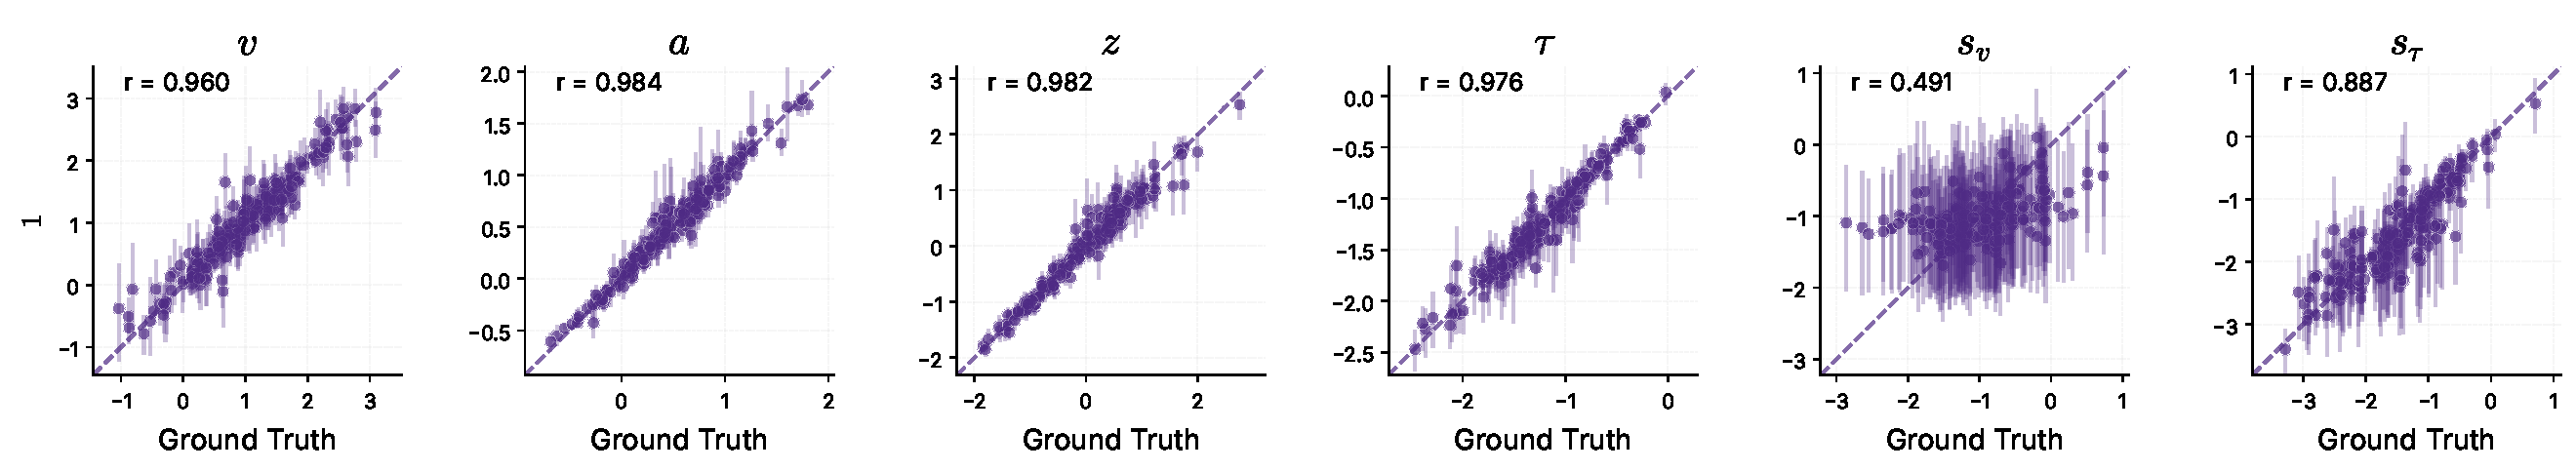
\includegraphics[width=\textwidth,height=0.3\textheight,keepaspectratio]{ddm/intercept_only/cf_recovery.pdf}\par\vspace{1ex}
  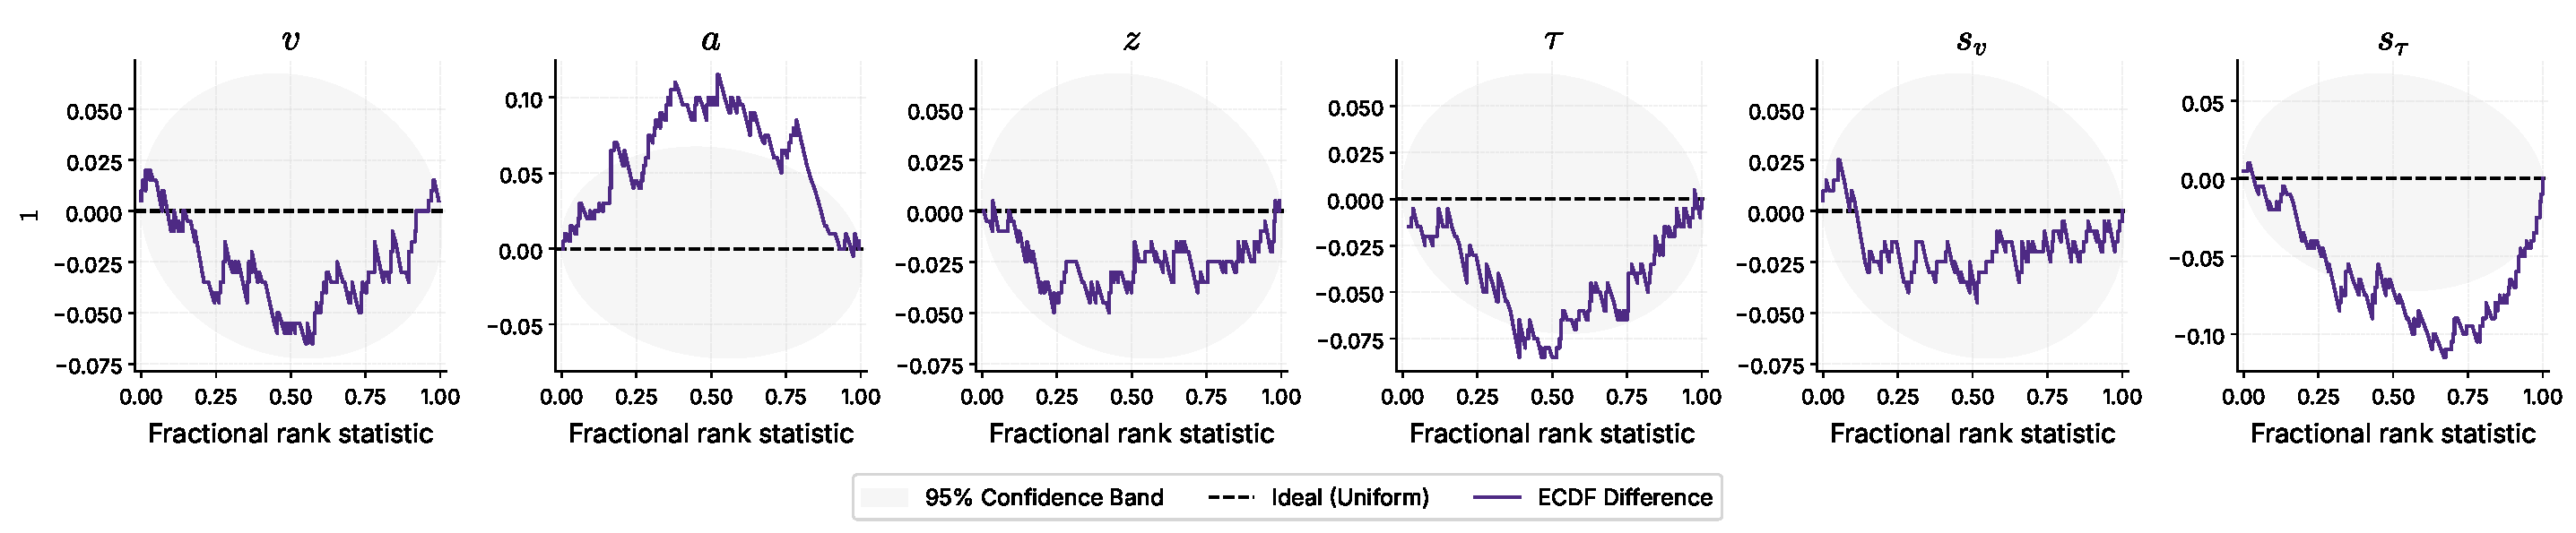
\includegraphics[width=\textwidth,height=0.3\textheight,keepaspectratio]{ddm/intercept_only/cf_ecdf.pdf}\par\vspace{1ex}
  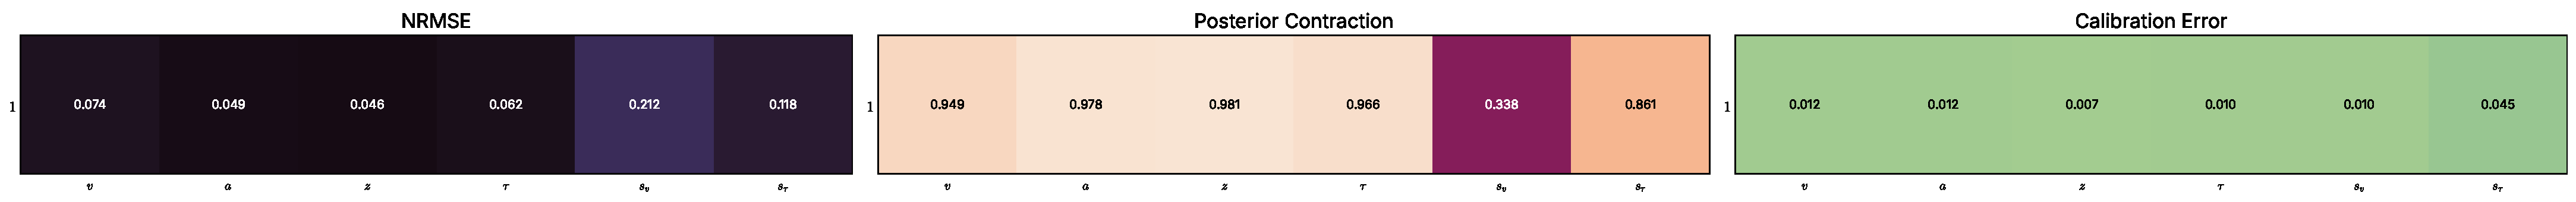
\includegraphics[width=\textwidth]{ddm/intercept_only/cf_metrics.pdf}
  \caption{\textbf{DDM, \emph{intercept-only} design: CogFormer.} Parameter recovery (top), calibration (middle) and summary metrics (bottom) on the 200 bench5 test datasets (500 trials each), from 200 posterior draws per dataset. CogFormer is a single network amortized over all three model families and all designs; each BayesFlow baseline is trained for one family and design alone, and both are evaluated on the same datasets. In every panel, columns are the model parameters and rows the coefficients of the design: the intercept ($1$) and, in regressed designs, the slopes on the continuous regressors $u_1$, $u_2$ and their product $u_1 u_2$; shading separates intercepts, main effects and interactions, and N/A marks coefficients the design does not contain. Values are on the unconstrained (link) scale on which both networks are trained; the contamination probability $\pi$ is estimated jointly but not shown. Top: posterior means (dots) against ground truth, with central 90\% credible intervals (bars); the dashed line is the identity and $r$ the Pearson correlation between posterior means and ground truth. Middle: empirical CDF of the fractional rank of the ground truth among the posterior draws (the share of draws below the truth), minus the uniform CDF. A calibrated posterior stays inside the grey band, the pointwise 95\% band for 200 uniform ranks, around the dashed zero line. A curve above zero throughout indicates overestimation, below zero underestimation; an inverted U indicates posteriors that are too wide, a U-shape overconfident ones. Bottom: per coefficient, on a common 0--1 colour scale: NRMSE, the root mean squared error of the posterior draws against the ground truth across datasets (median over draws), divided by the range of the ground-truth values (lower is better); posterior contraction, one minus the ratio of posterior variance to the variance of the ground-truth values, clipped to $[0, 1]$ and taken as the median over datasets (higher is better); and calibration error, the median absolute difference between empirical and nominal coverage of central credible intervals at 20 levels from 0.5\% to 99.5\% (lower is better). Every estimated parameter enters as an intercept only (6 coefficients shown). All subsequent figures in this section (Figures~\ref{fig:app1-ddm-intercept-only-bf}--\ref{fig:app1-cdm-interaction-bf}) follow this layout and encoding.}
  \label{fig:app1-ddm-intercept-only-cf}
\end{figure}

\begin{figure}[p]
  \centering
  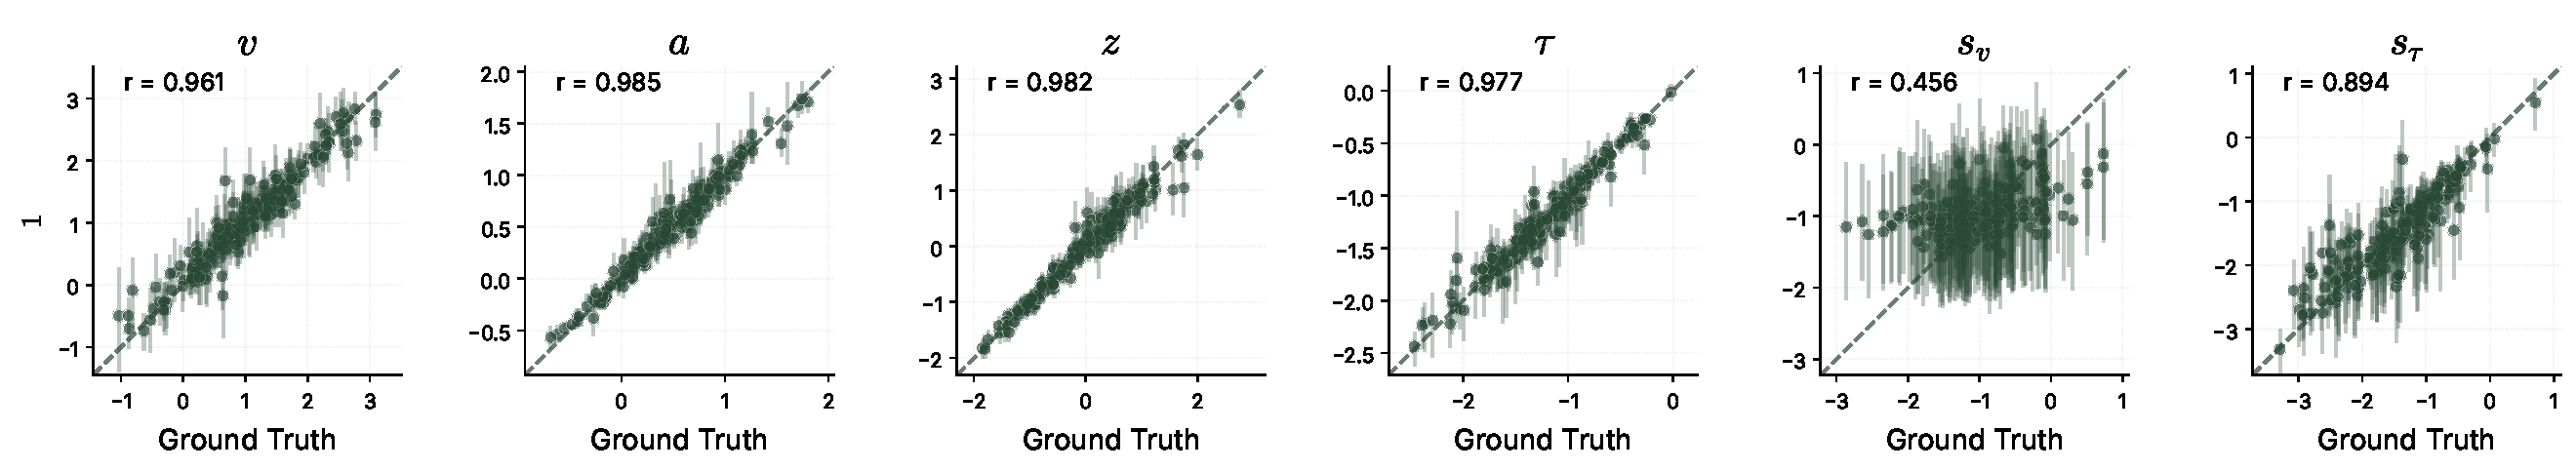
\includegraphics[width=\textwidth,height=0.3\textheight,keepaspectratio]{ddm/intercept_only/bf_recovery.pdf}\par\vspace{1ex}
  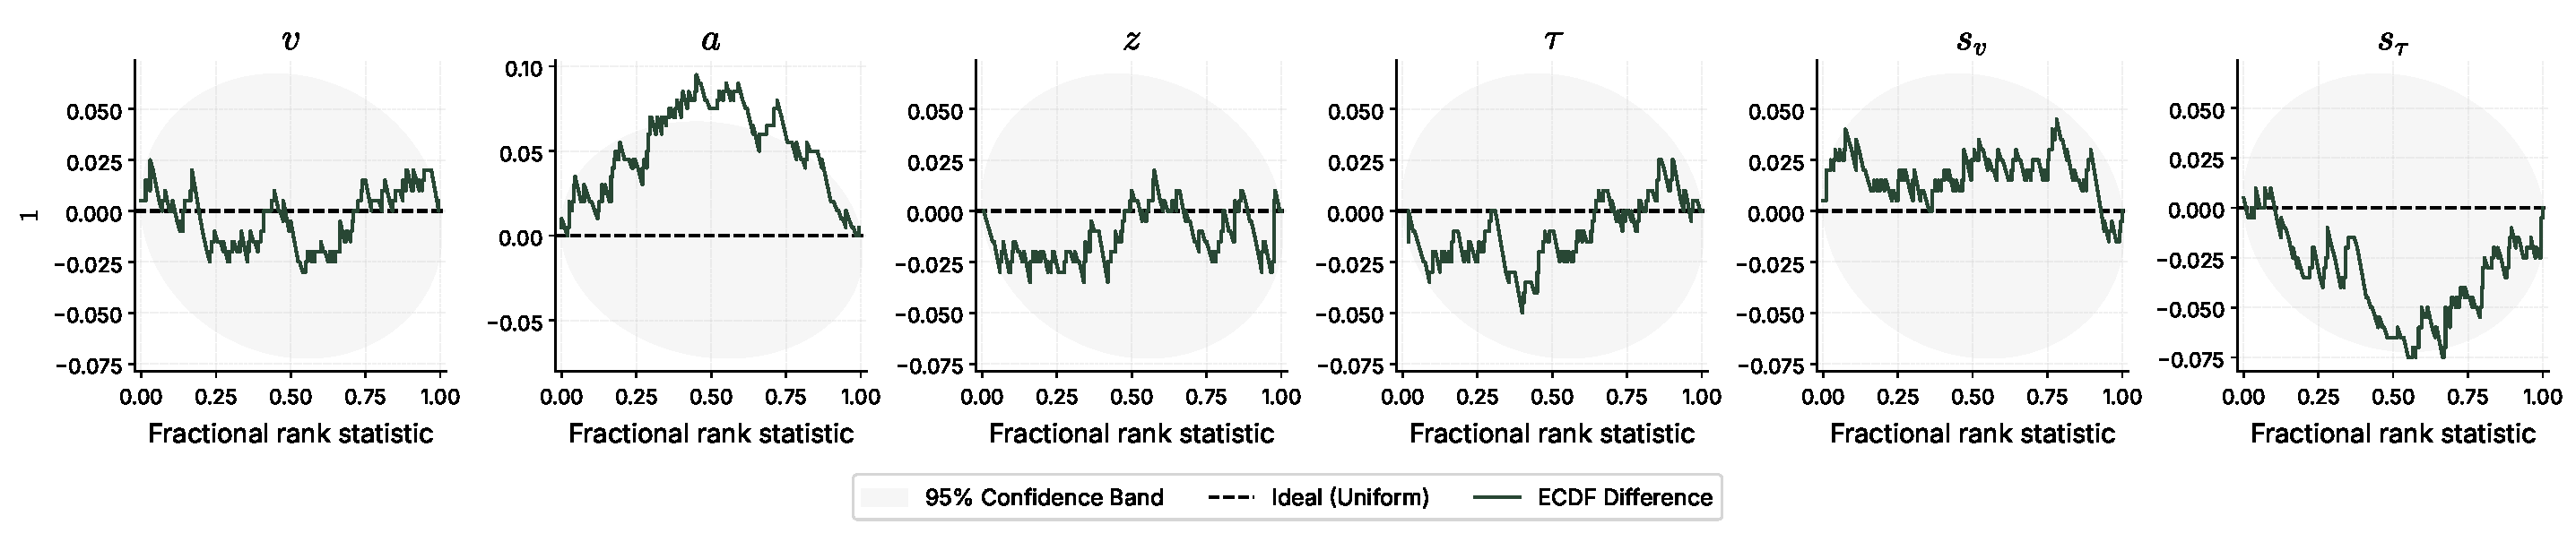
\includegraphics[width=\textwidth,height=0.3\textheight,keepaspectratio]{ddm/intercept_only/bf_ecdf.pdf}\par\vspace{1ex}
  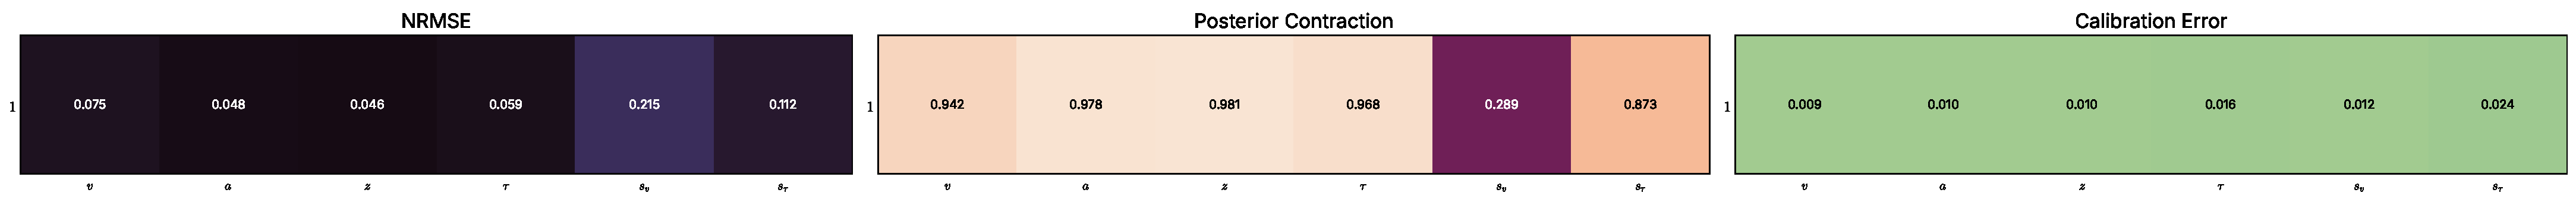
\includegraphics[width=\textwidth]{ddm/intercept_only/bf_metrics.pdf}
  \caption{\textbf{DDM, \emph{intercept-only} design: BayesFlow baseline.} Recovery (top), calibration (middle), metrics (bottom). Every estimated parameter enters as an intercept only (6 coefficients shown). Layout and encoding as in Figure~\ref{fig:app1-ddm-intercept-only-cf}.}
  \label{fig:app1-ddm-intercept-only-bf}
\end{figure}

\begin{figure}[p]
  \centering
  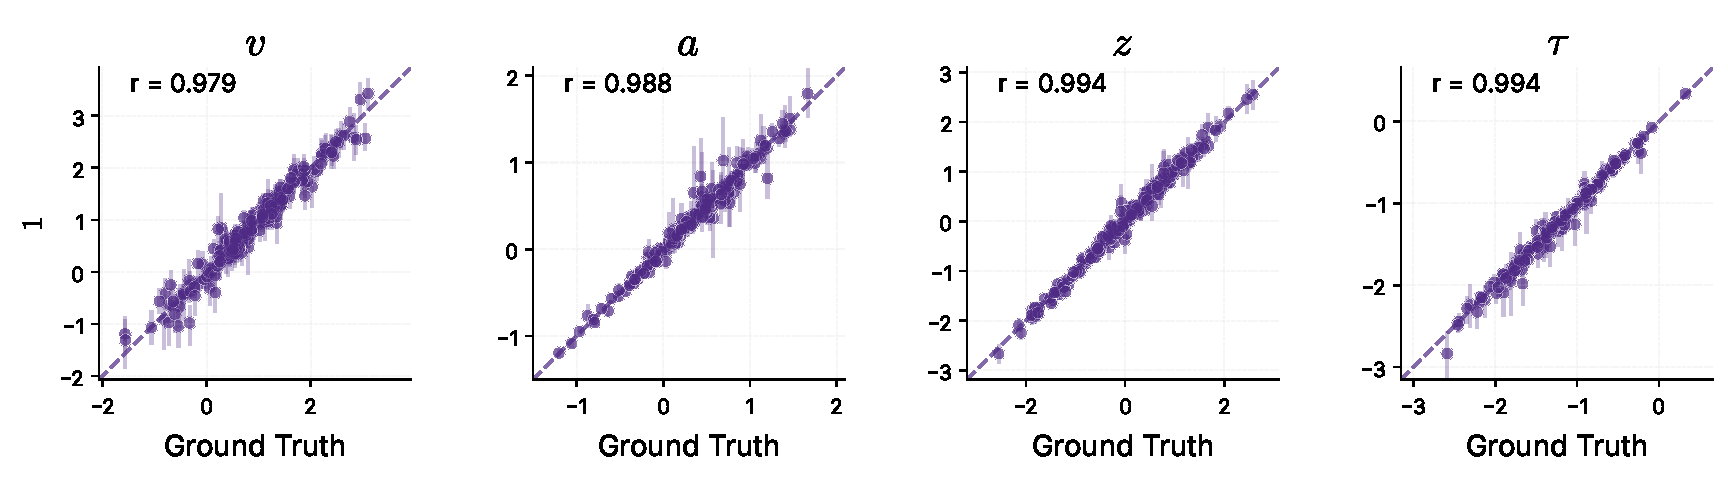
\includegraphics[width=\textwidth,height=0.3\textheight,keepaspectratio]{ddm/fixed/cf_recovery.pdf}\par\vspace{1ex}
  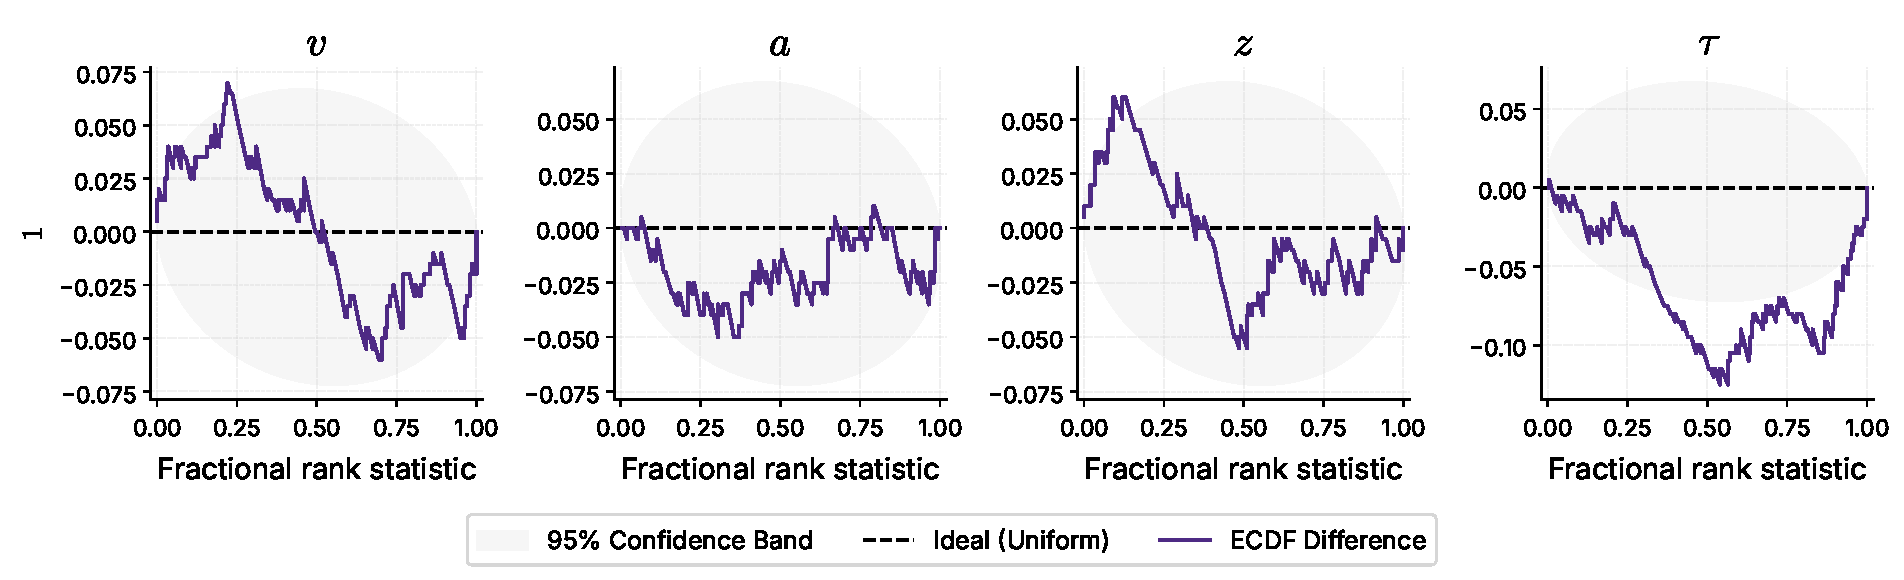
\includegraphics[width=\textwidth,height=0.3\textheight,keepaspectratio]{ddm/fixed/cf_ecdf.pdf}\par\vspace{1ex}
  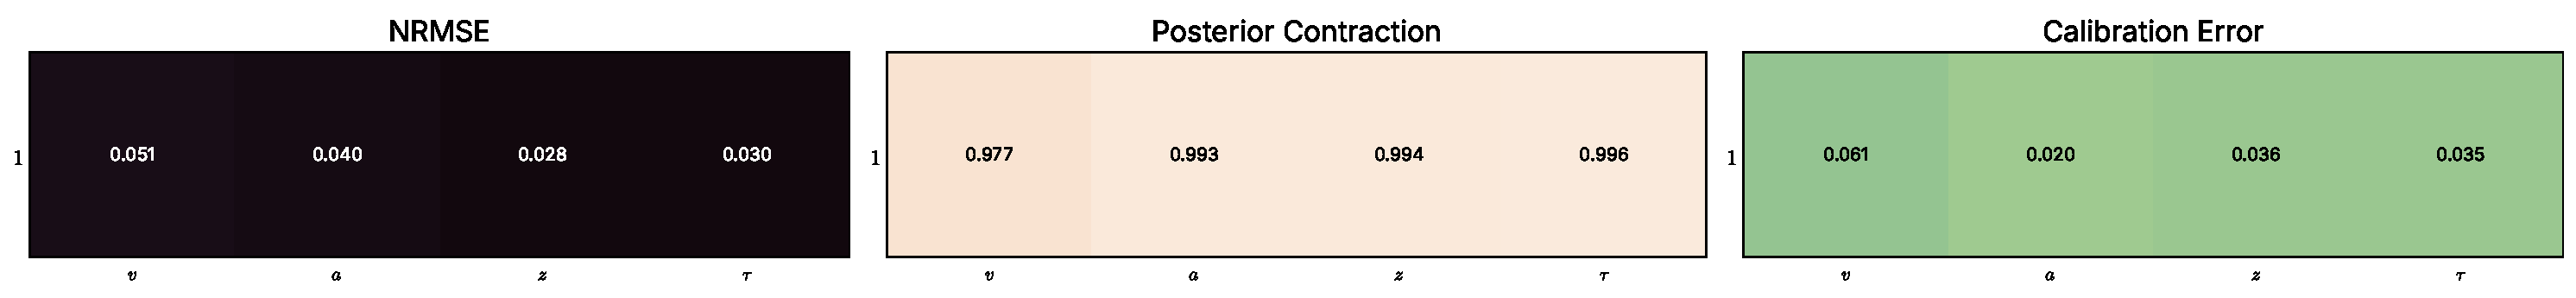
\includegraphics[width=\textwidth]{ddm/fixed/cf_metrics.pdf}
  \caption{\textbf{DDM, \emph{fixed} design: CogFormer.} Recovery (top), calibration (middle), metrics (bottom). $s_v$ and $s_\tau$ are fixed at 0 and not estimated; every estimated parameter enters as an intercept only (4 coefficients shown). Layout and encoding as in Figure~\ref{fig:app1-ddm-intercept-only-cf}.}
  \label{fig:app1-ddm-fixed-cf}
\end{figure}

\begin{figure}[p]
  \centering
  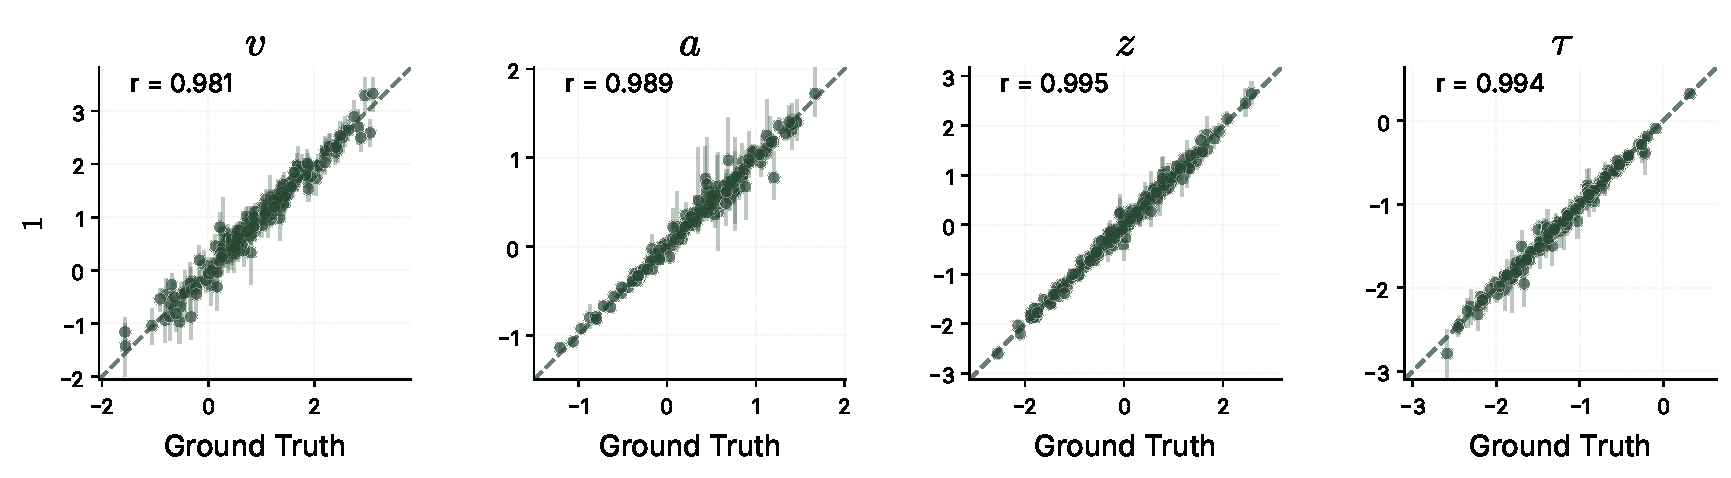
\includegraphics[width=\textwidth,height=0.3\textheight,keepaspectratio]{ddm/fixed/bf_recovery.pdf}\par\vspace{1ex}
  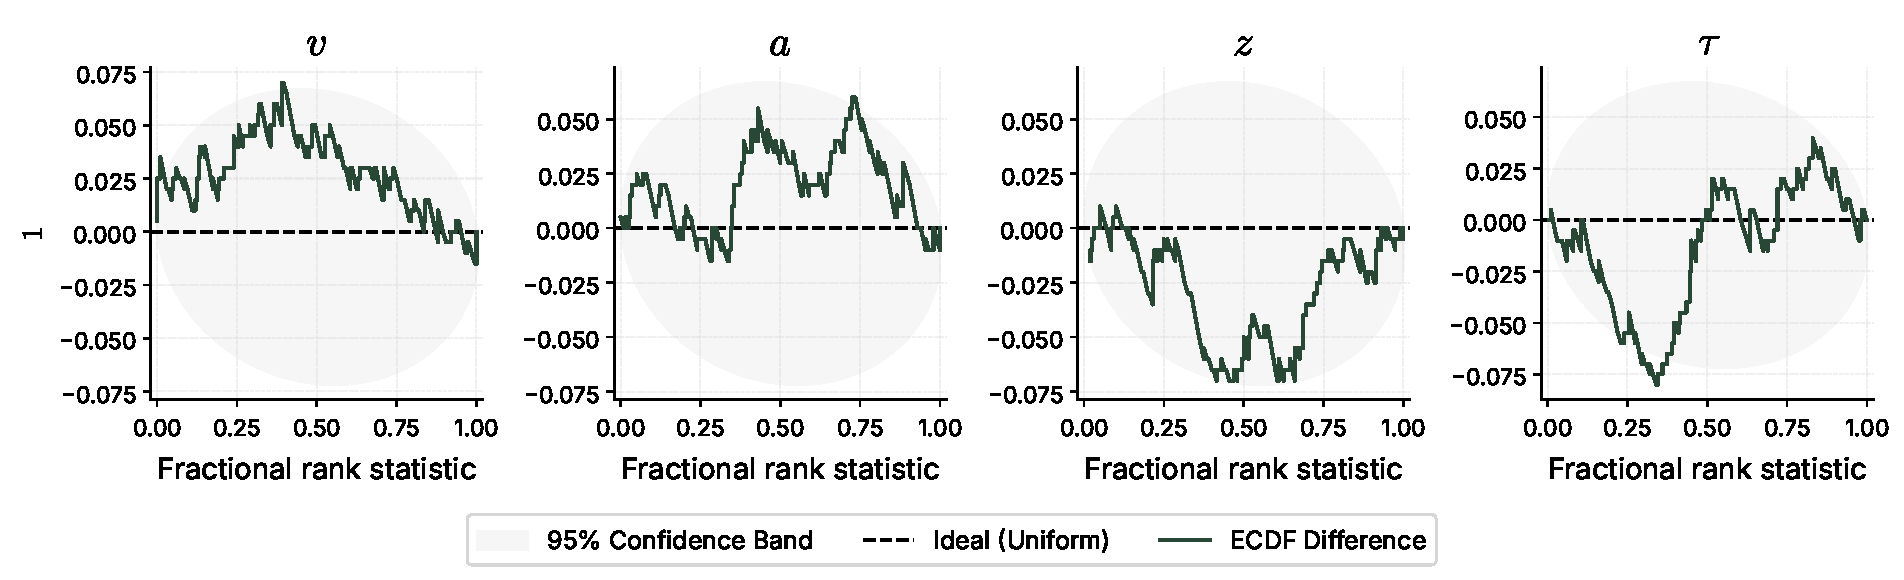
\includegraphics[width=\textwidth,height=0.3\textheight,keepaspectratio]{ddm/fixed/bf_ecdf.pdf}\par\vspace{1ex}
  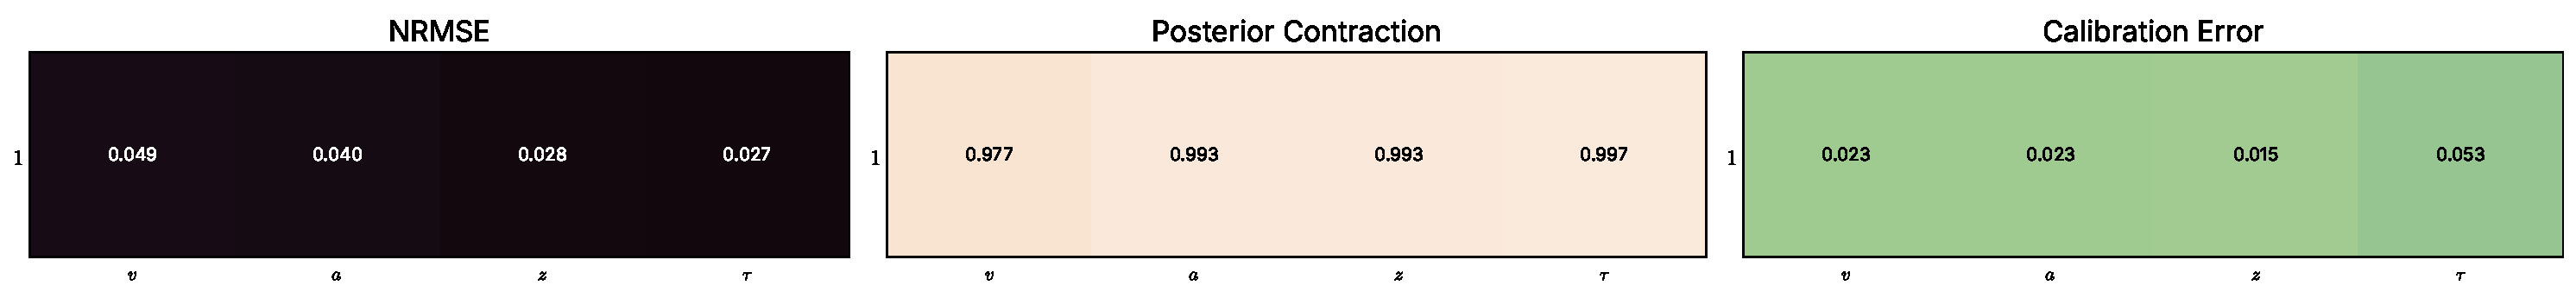
\includegraphics[width=\textwidth]{ddm/fixed/bf_metrics.pdf}
  \caption{\textbf{DDM, \emph{fixed} design: BayesFlow baseline.} Recovery (top), calibration (middle), metrics (bottom). $s_v$ and $s_\tau$ are fixed at 0 and not estimated; every estimated parameter enters as an intercept only (4 coefficients shown). Layout and encoding as in Figure~\ref{fig:app1-ddm-intercept-only-cf}.}
  \label{fig:app1-ddm-fixed-bf}
\end{figure}

\begin{figure}[p]
  \centering
  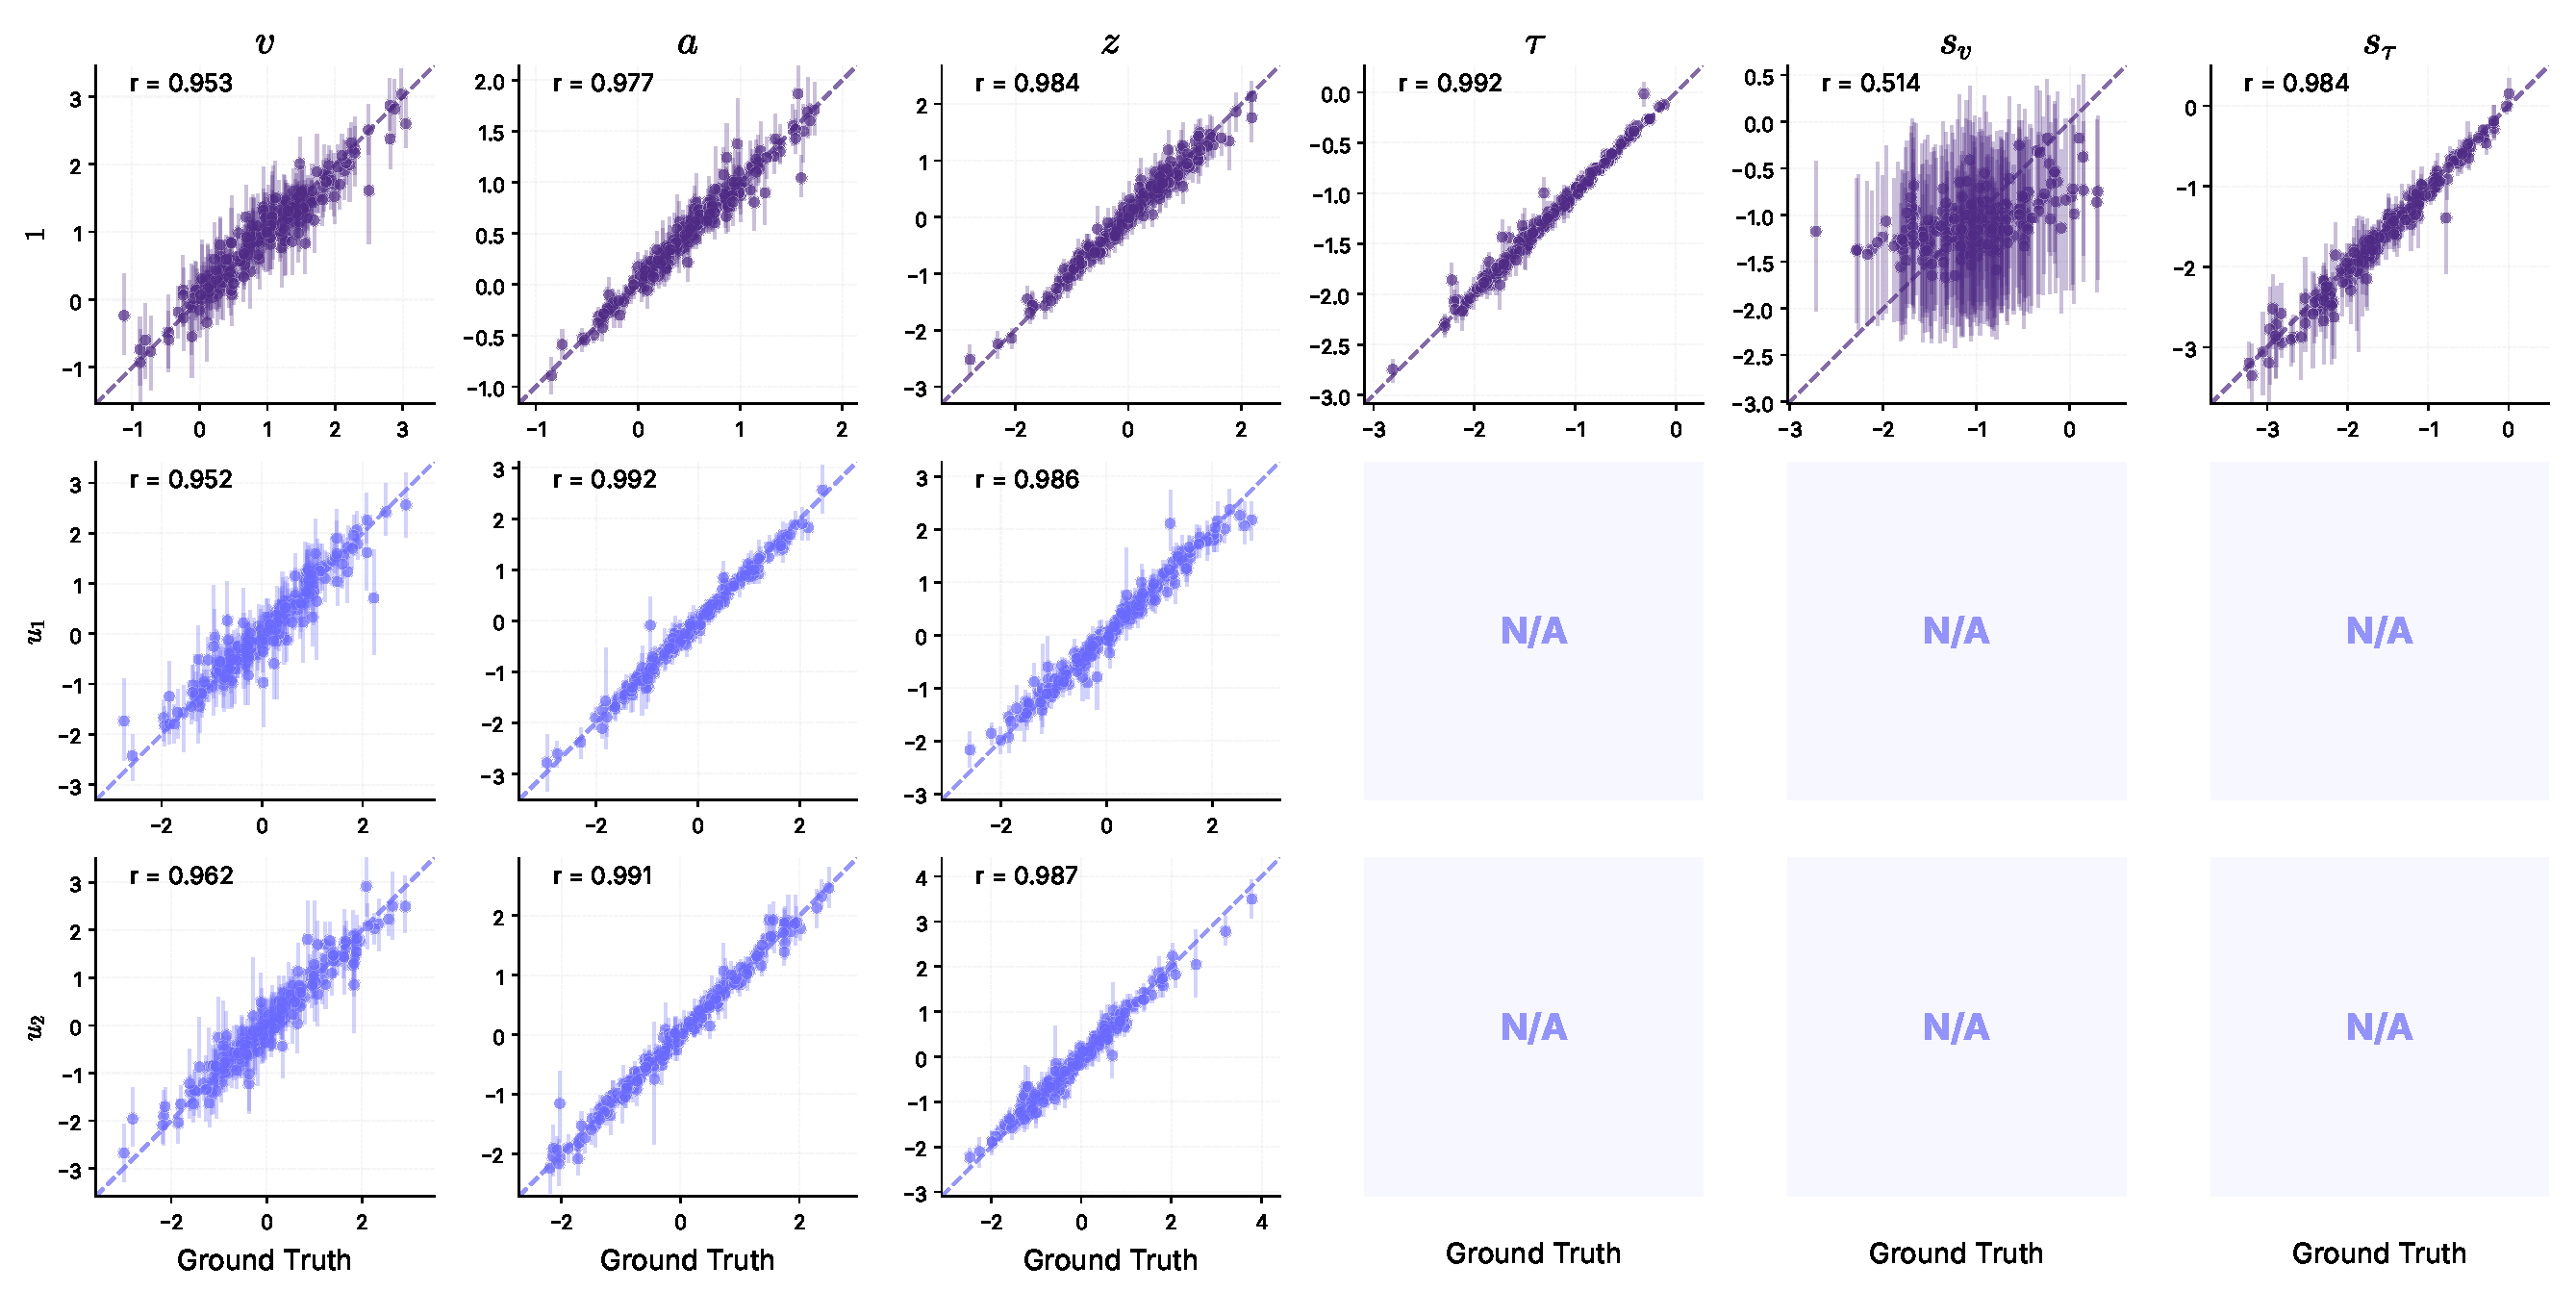
\includegraphics[width=\textwidth,height=0.3\textheight,keepaspectratio]{ddm/regressed/cf_recovery.pdf}\par\vspace{1ex}
  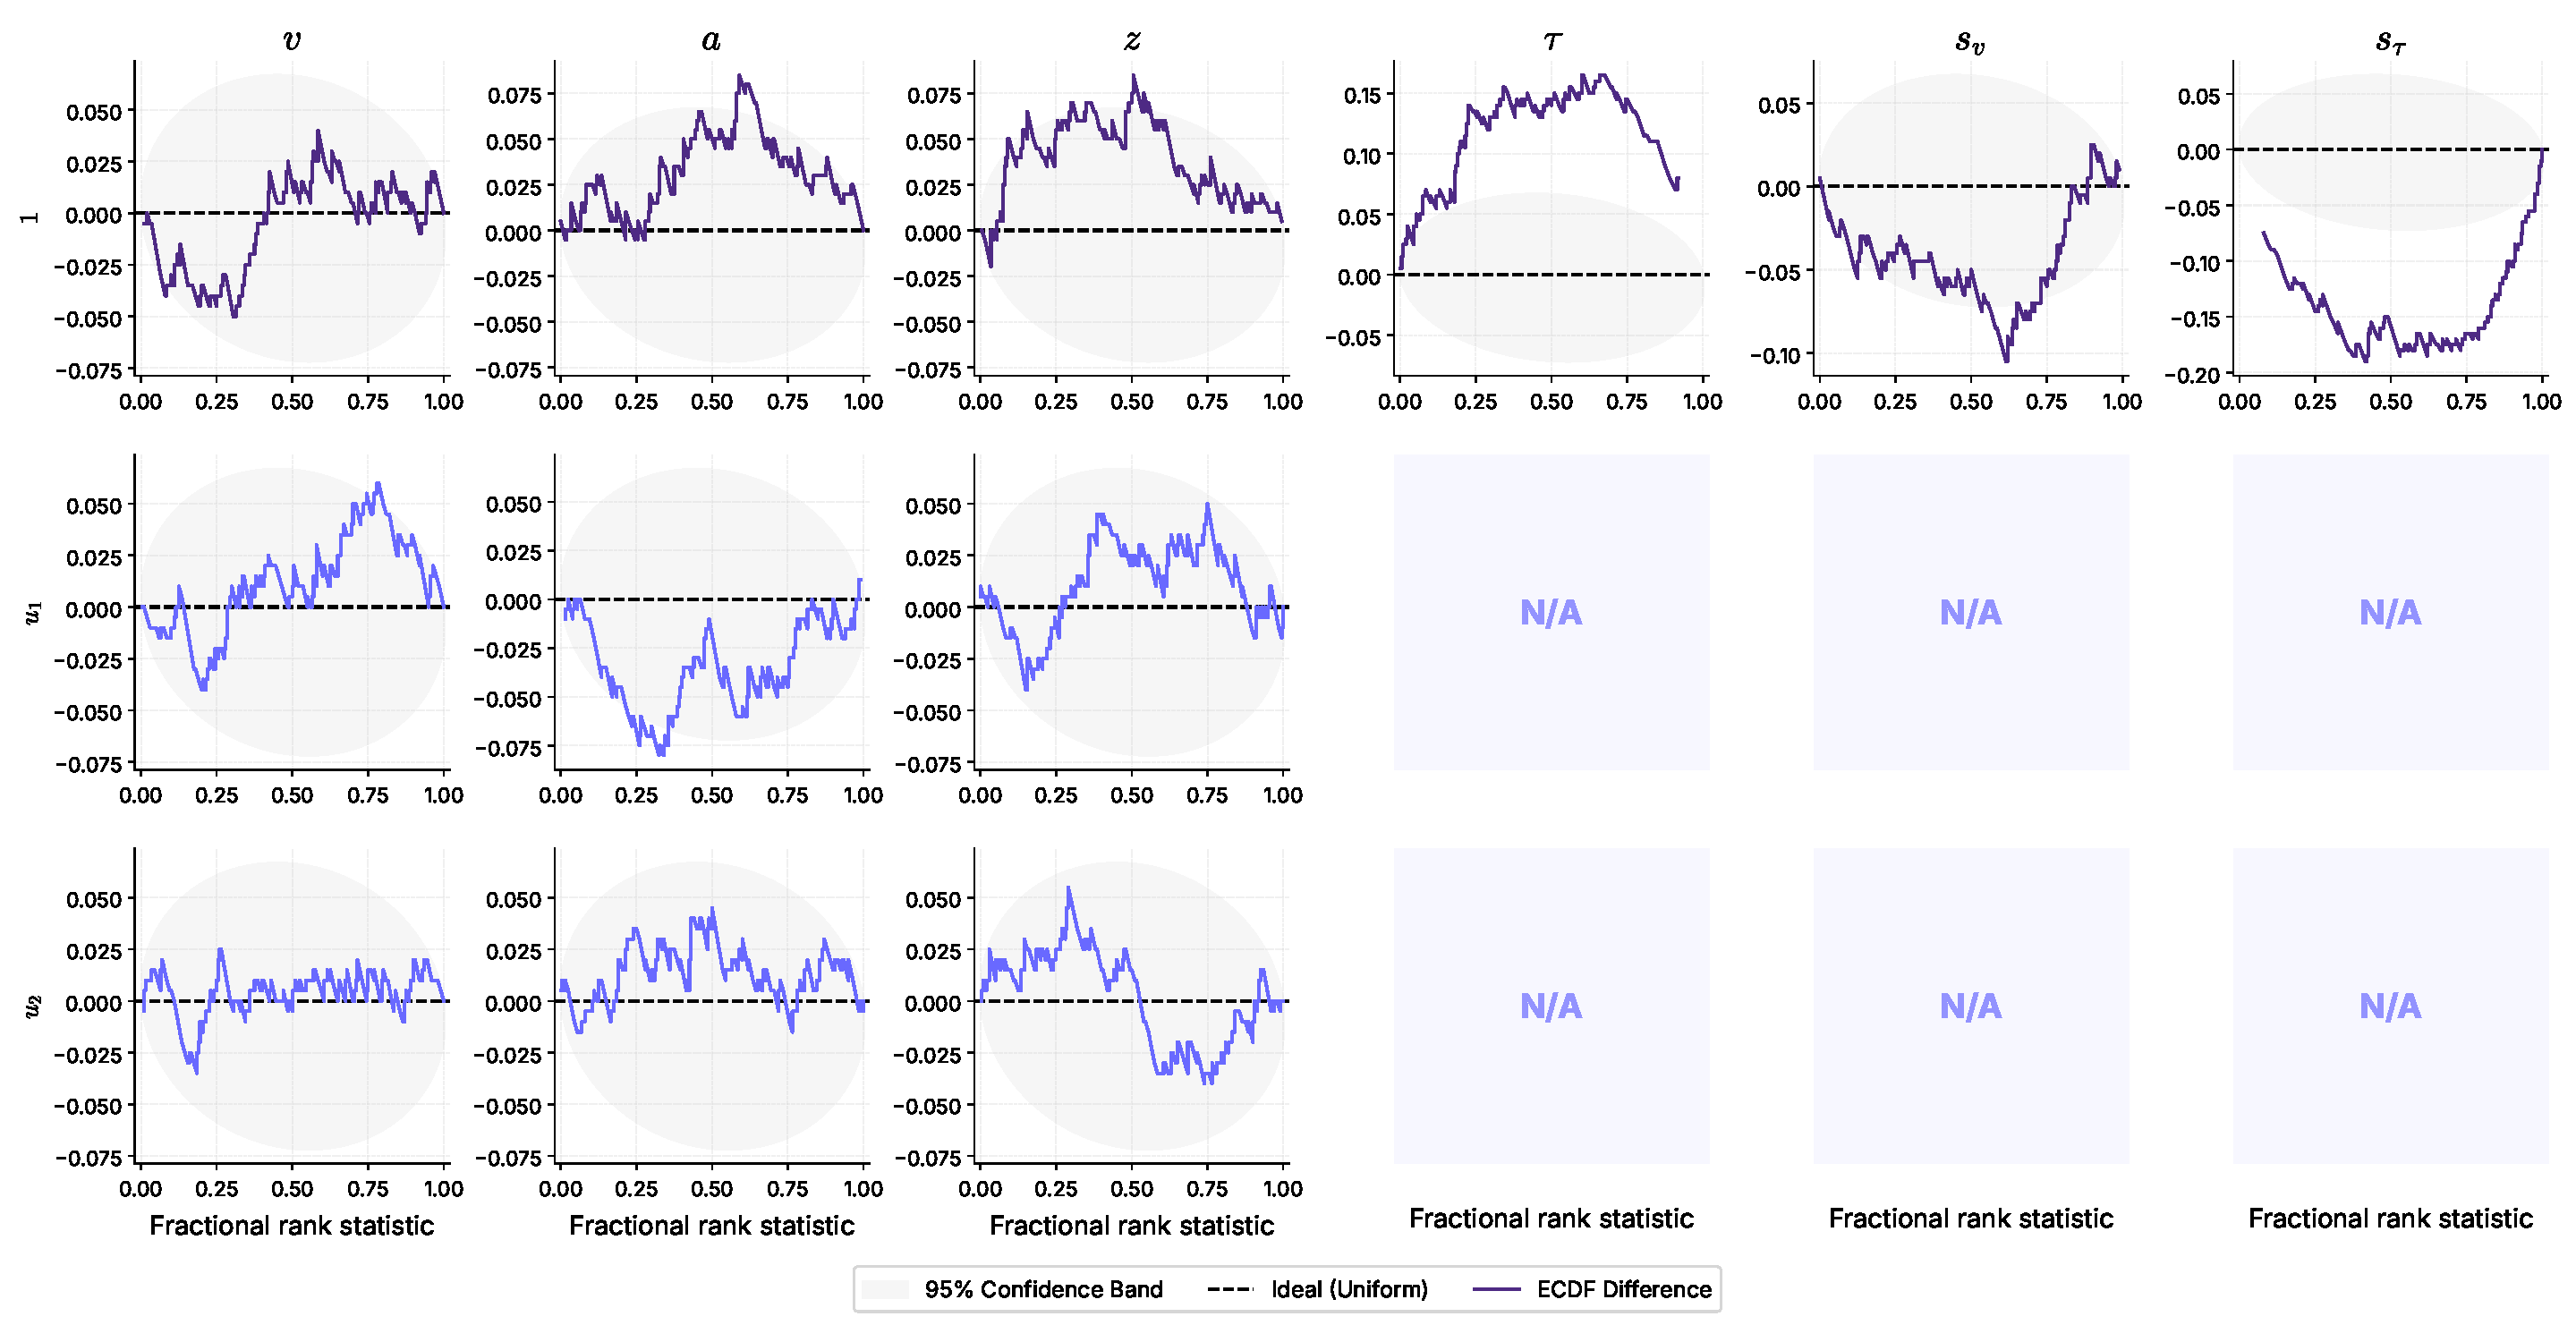
\includegraphics[width=\textwidth,height=0.3\textheight,keepaspectratio]{ddm/regressed/cf_ecdf.pdf}\par\vspace{1ex}
  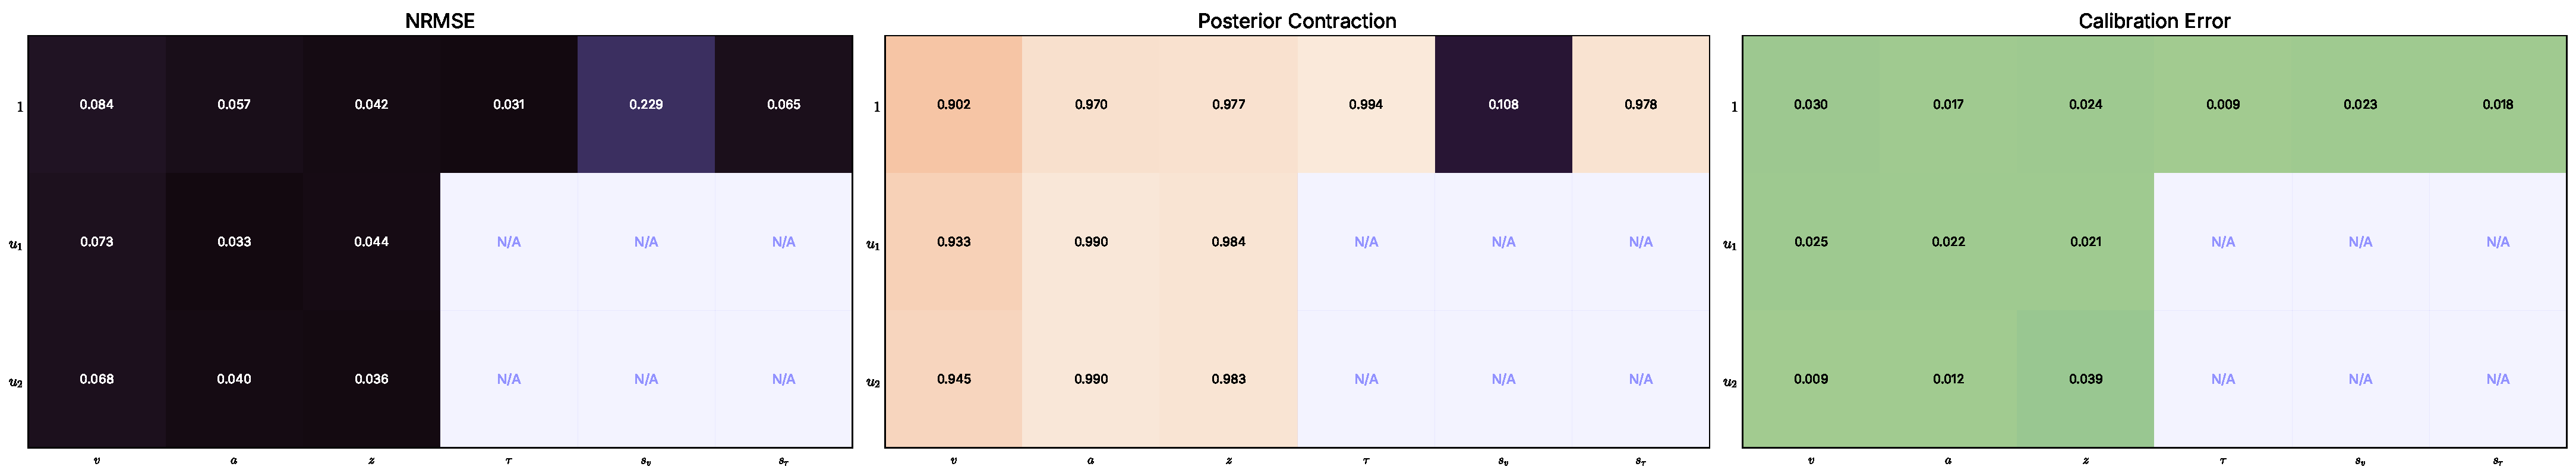
\includegraphics[width=\textwidth]{ddm/regressed/cf_metrics.pdf}
  \caption{\textbf{DDM, \emph{regressed} design: CogFormer.} Recovery (top), calibration (middle), metrics (bottom). $v$, $a$ and $z$ carry slopes on $u_1$ and $u_2$ (12 coefficients shown). Layout and encoding as in Figure~\ref{fig:app1-ddm-intercept-only-cf}.}
  \label{fig:app1-ddm-regressed-cf}
\end{figure}

\begin{figure}[p]
  \centering
  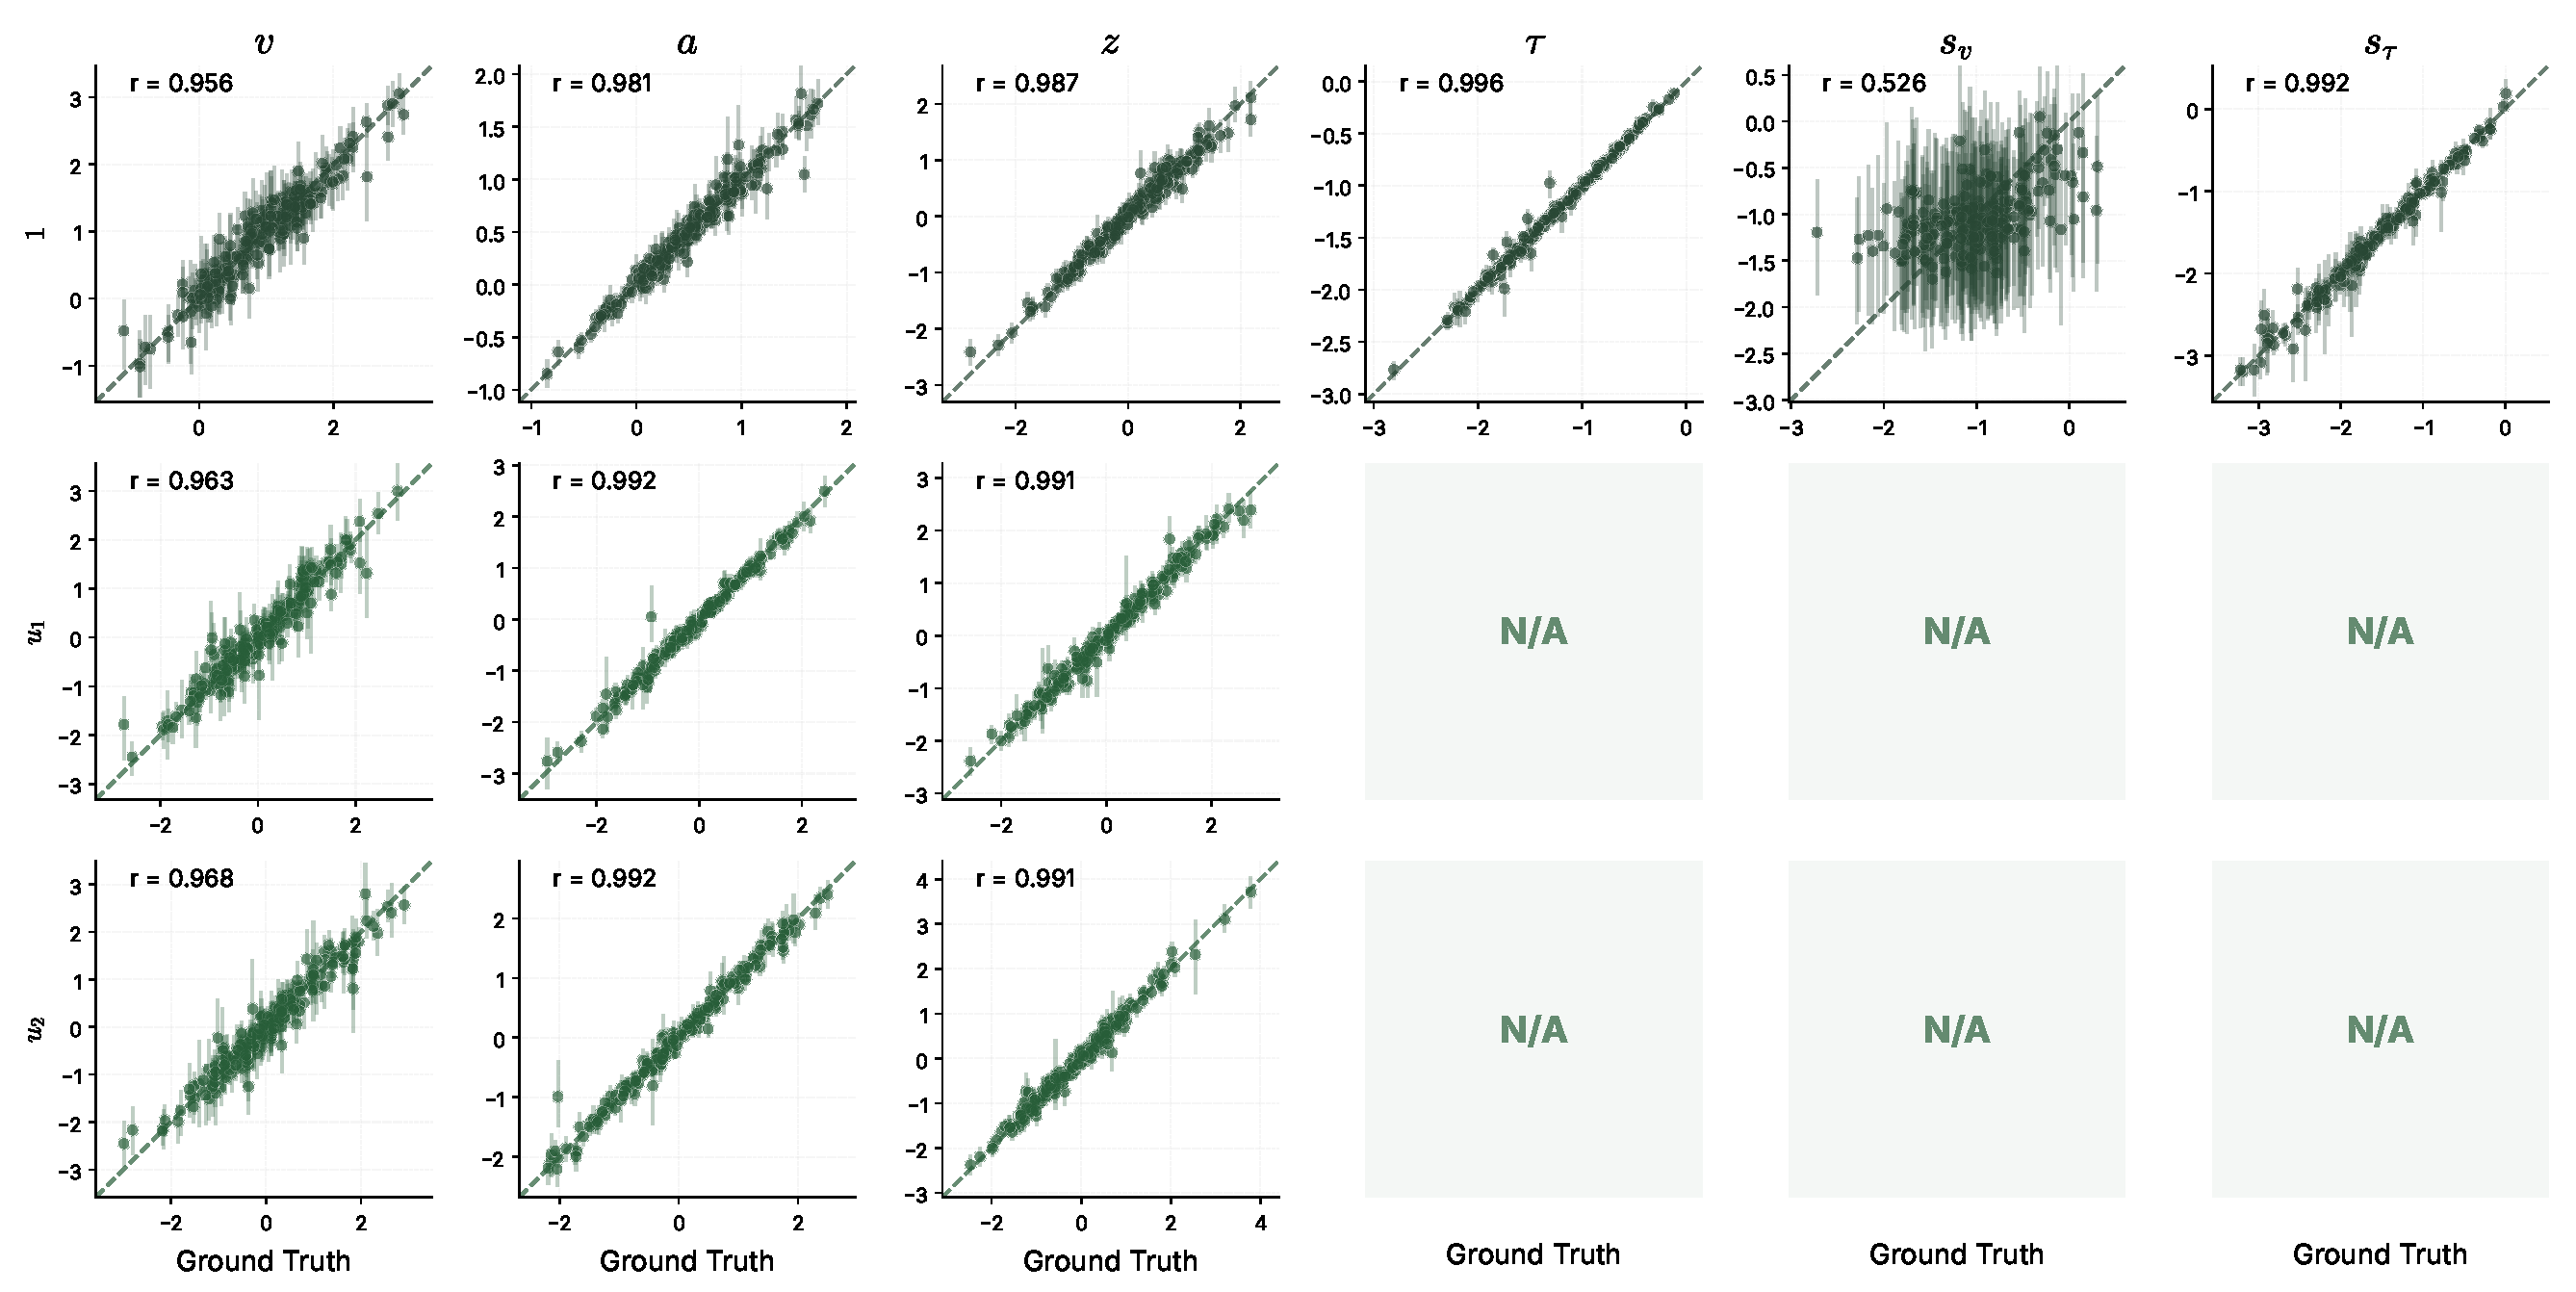
\includegraphics[width=\textwidth,height=0.3\textheight,keepaspectratio]{ddm/regressed/bf_recovery.pdf}\par\vspace{1ex}
  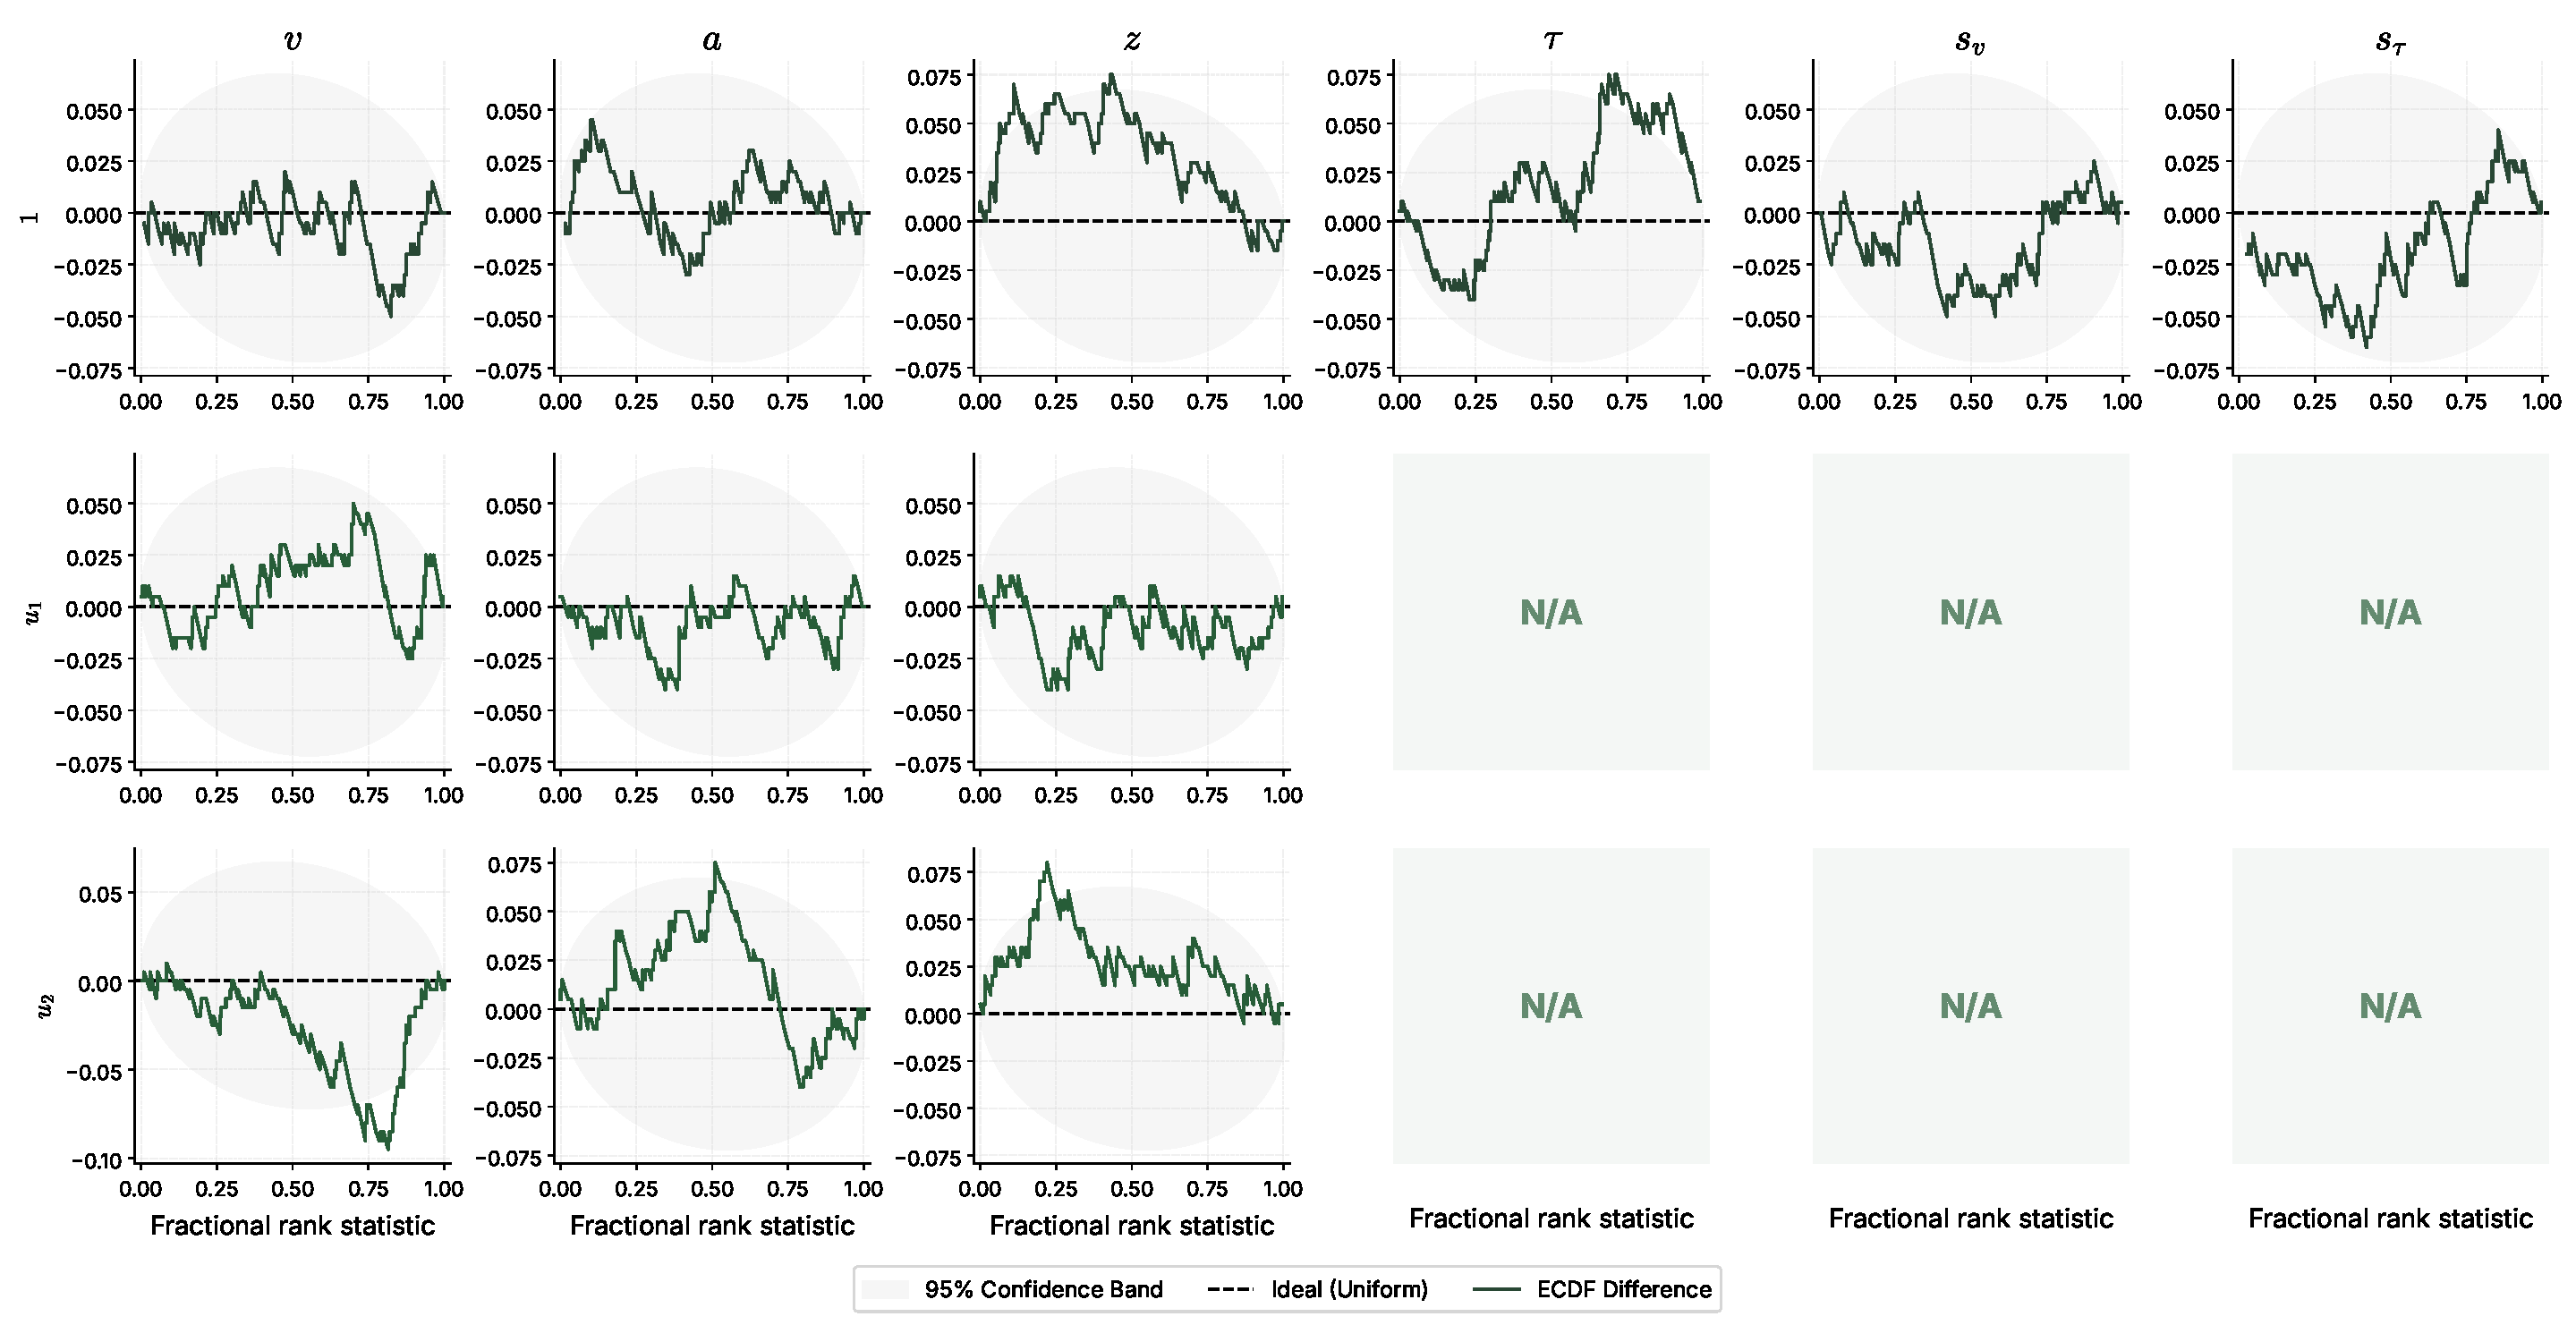
\includegraphics[width=\textwidth,height=0.3\textheight,keepaspectratio]{ddm/regressed/bf_ecdf.pdf}\par\vspace{1ex}
  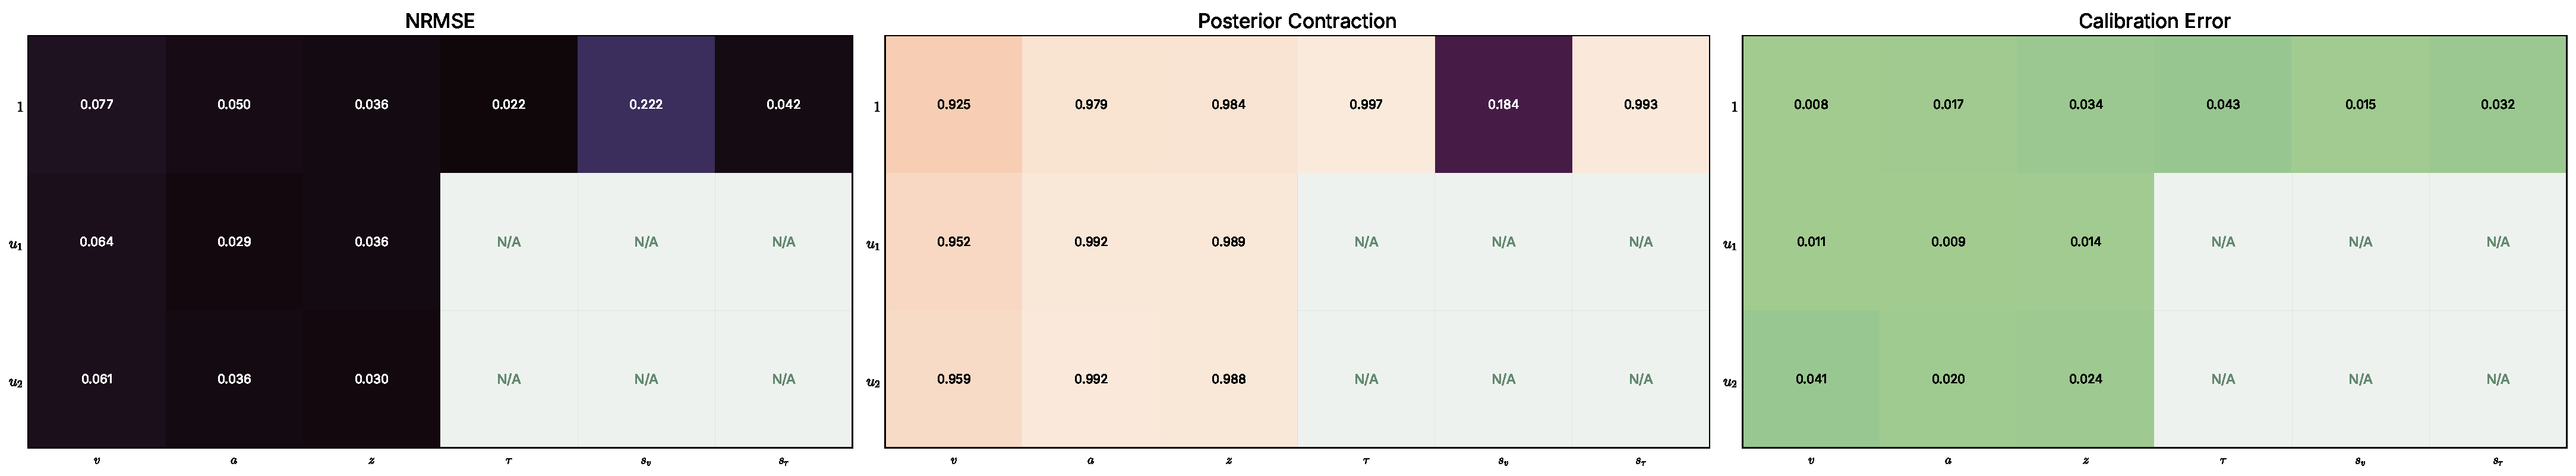
\includegraphics[width=\textwidth]{ddm/regressed/bf_metrics.pdf}
  \caption{\textbf{DDM, \emph{regressed} design: BayesFlow baseline.} Recovery (top), calibration (middle), metrics (bottom). $v$, $a$ and $z$ carry slopes on $u_1$ and $u_2$ (12 coefficients shown). Layout and encoding as in Figure~\ref{fig:app1-ddm-intercept-only-cf}.}
  \label{fig:app1-ddm-regressed-bf}
\end{figure}

\begin{figure}[p]
  \centering
  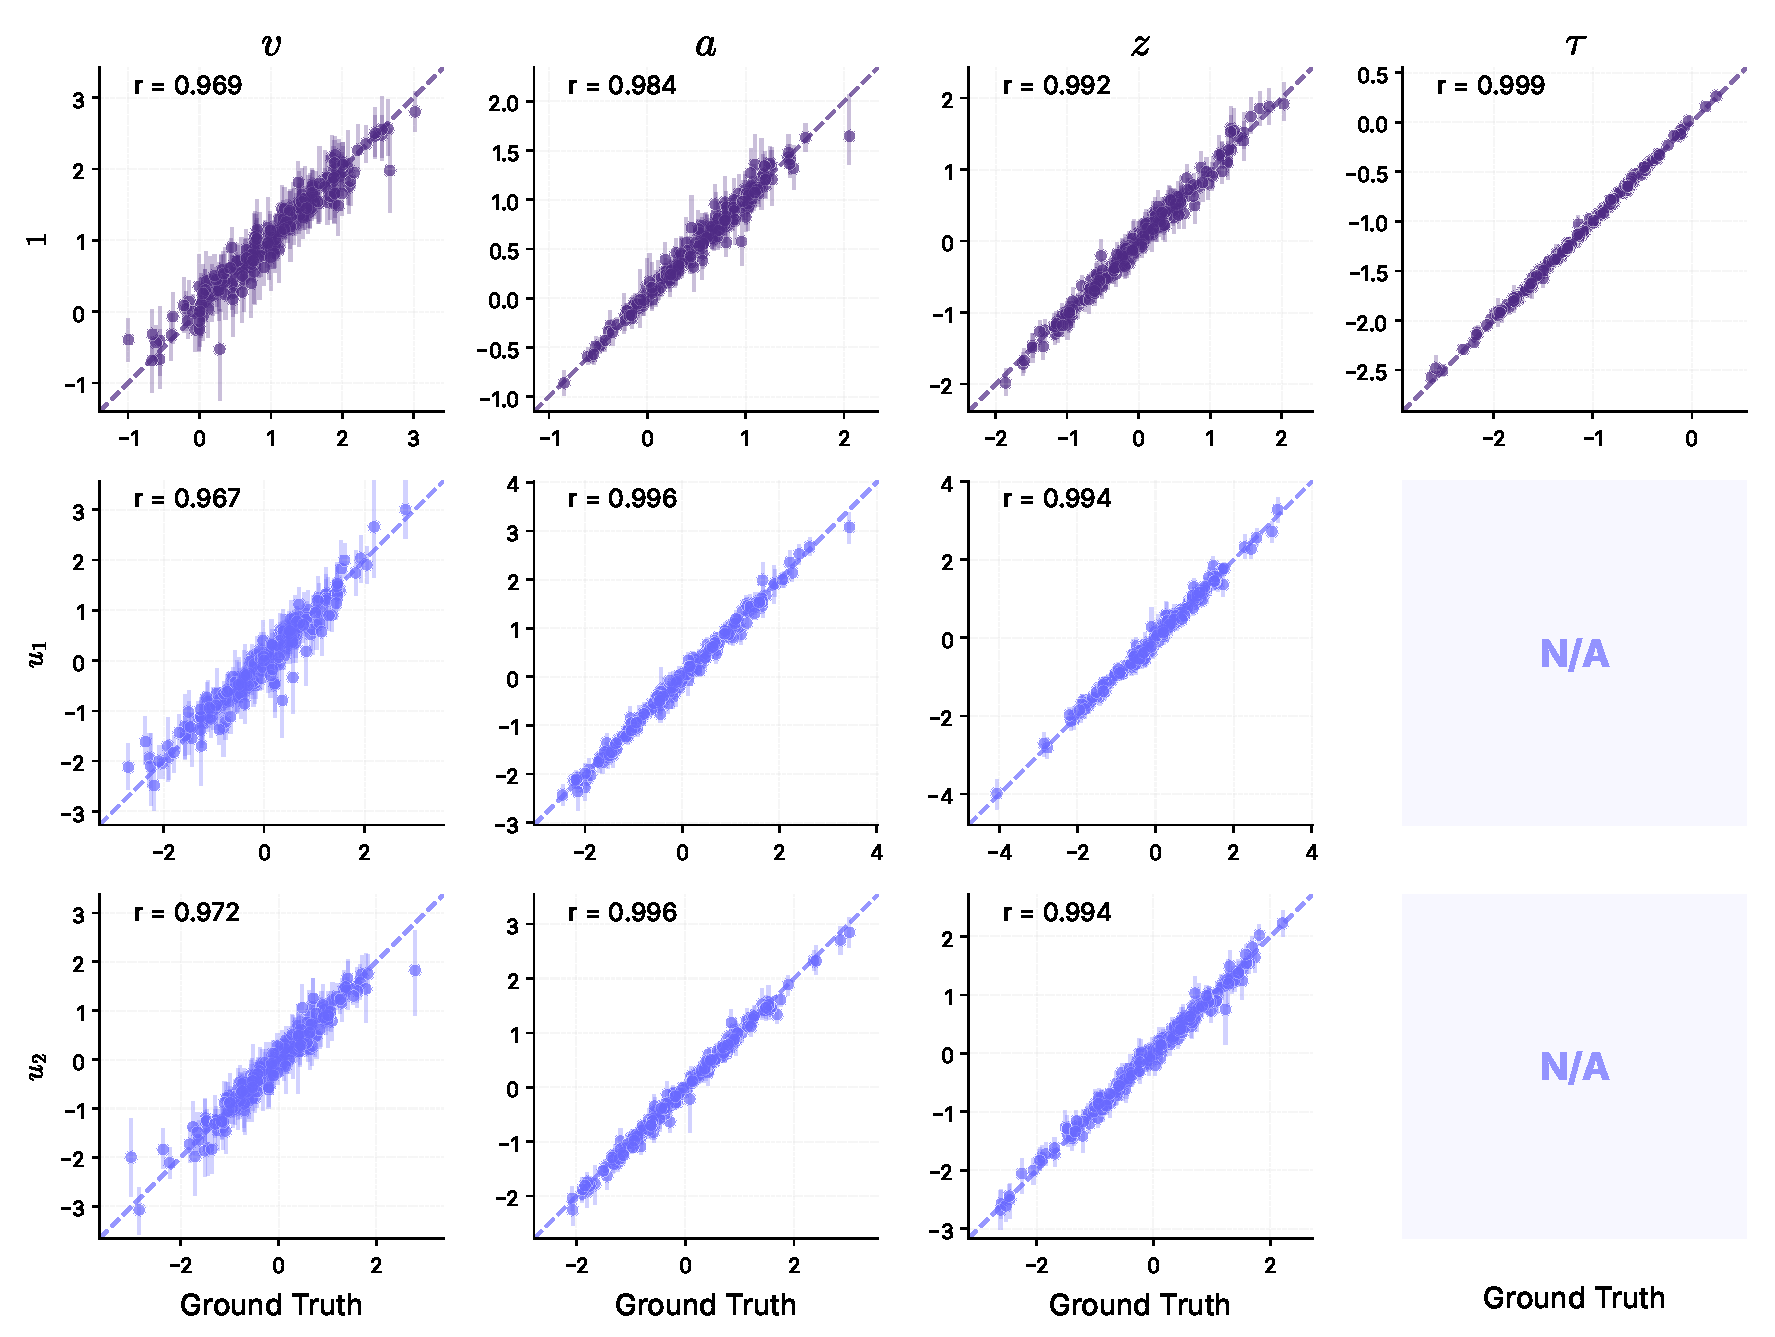
\includegraphics[width=\textwidth,height=0.3\textheight,keepaspectratio]{ddm/fixed_regressed/cf_recovery.pdf}\par\vspace{1ex}
  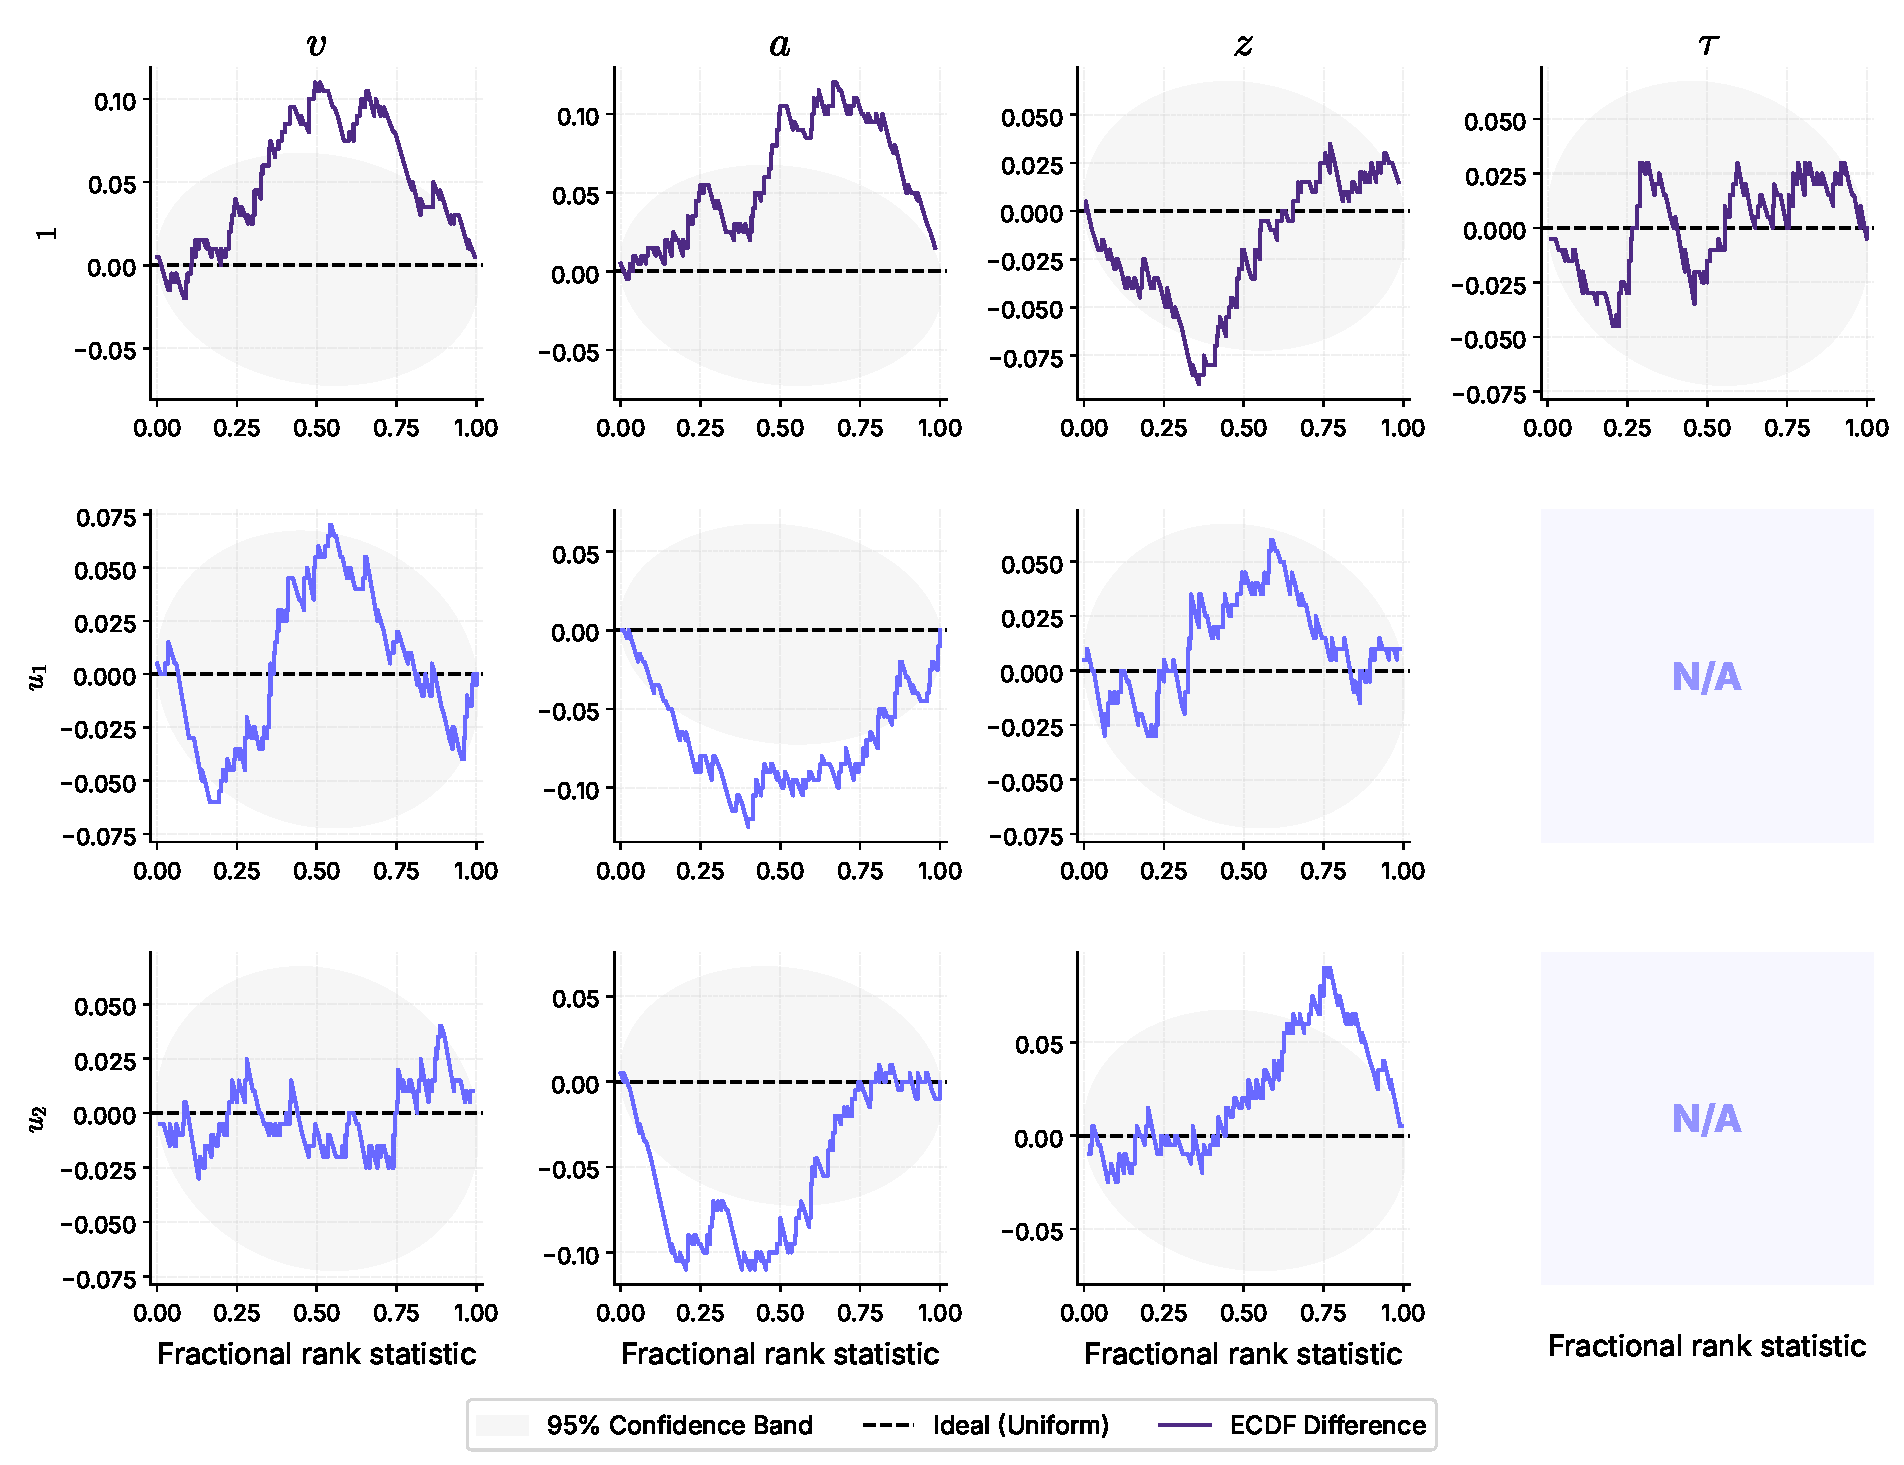
\includegraphics[width=\textwidth,height=0.3\textheight,keepaspectratio]{ddm/fixed_regressed/cf_ecdf.pdf}\par\vspace{1ex}
  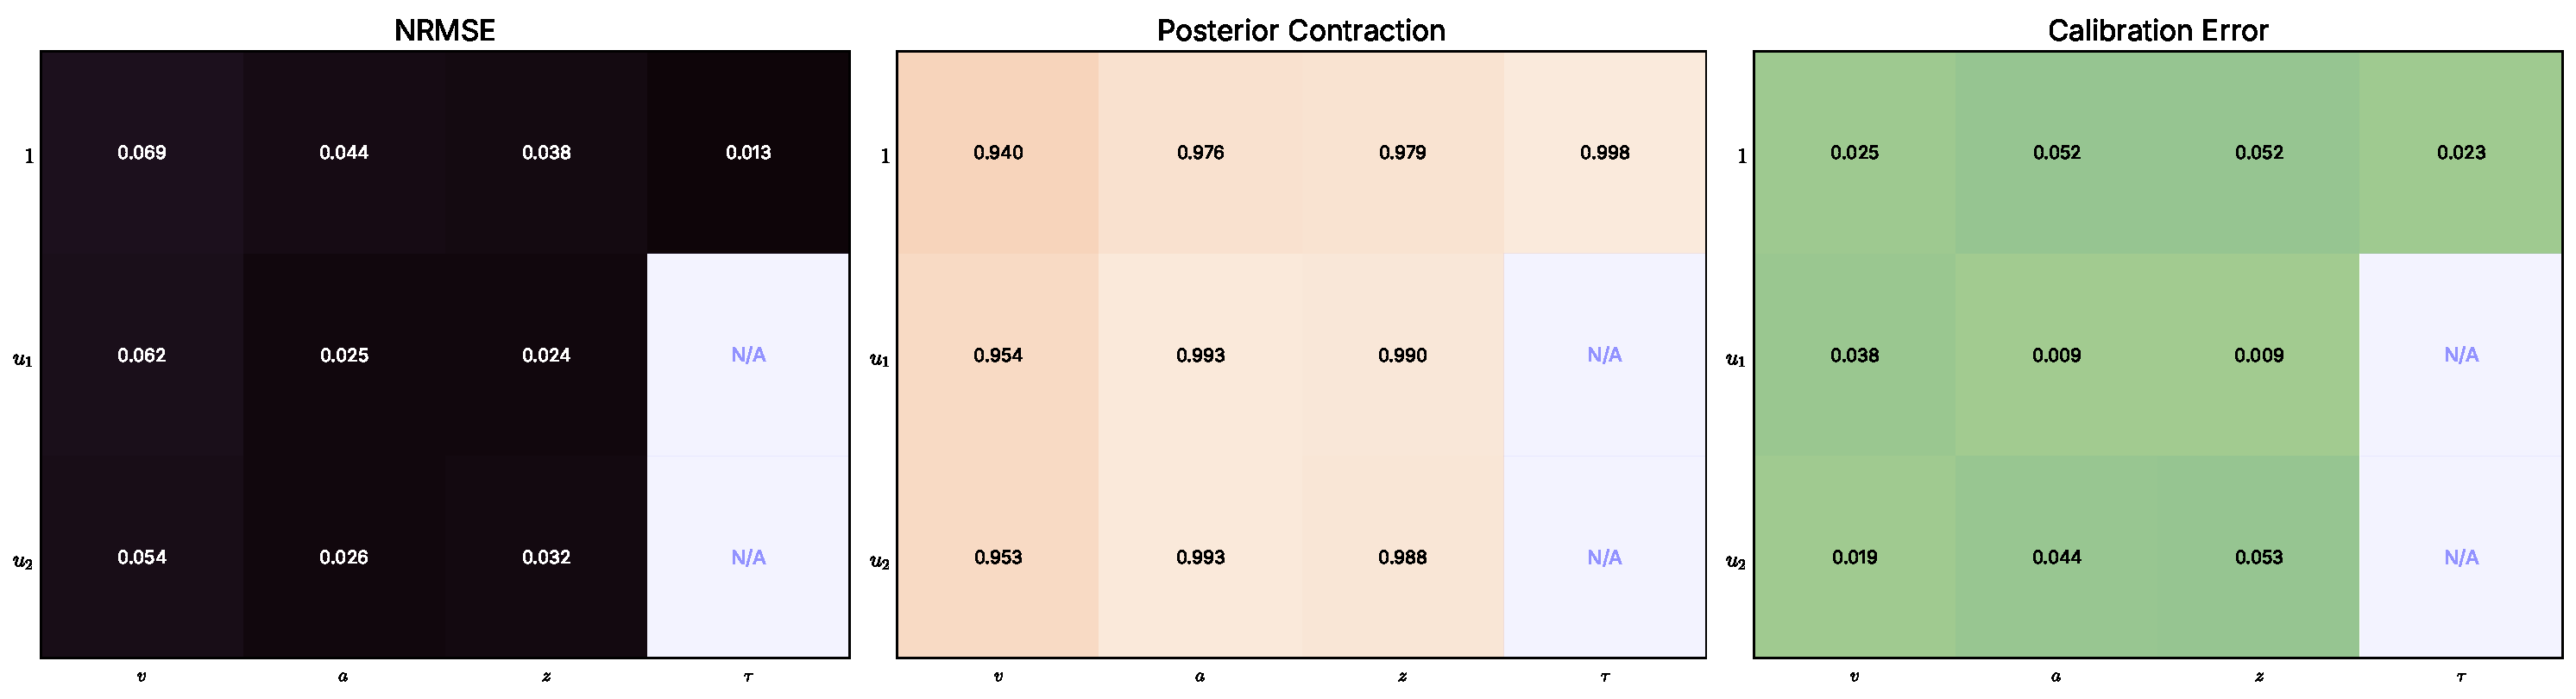
\includegraphics[width=\textwidth]{ddm/fixed_regressed/cf_metrics.pdf}
  \caption{\textbf{DDM, \emph{fixed + regressed} design: CogFormer.} Recovery (top), calibration (middle), metrics (bottom). $s_v$ and $s_\tau$ are fixed at 0 and not estimated; $v$, $a$ and $z$ carry slopes on $u_1$ and $u_2$ (10 coefficients shown). Layout and encoding as in Figure~\ref{fig:app1-ddm-intercept-only-cf}.}
  \label{fig:app1-ddm-fixed-regressed-cf}
\end{figure}

\begin{figure}[p]
  \centering
  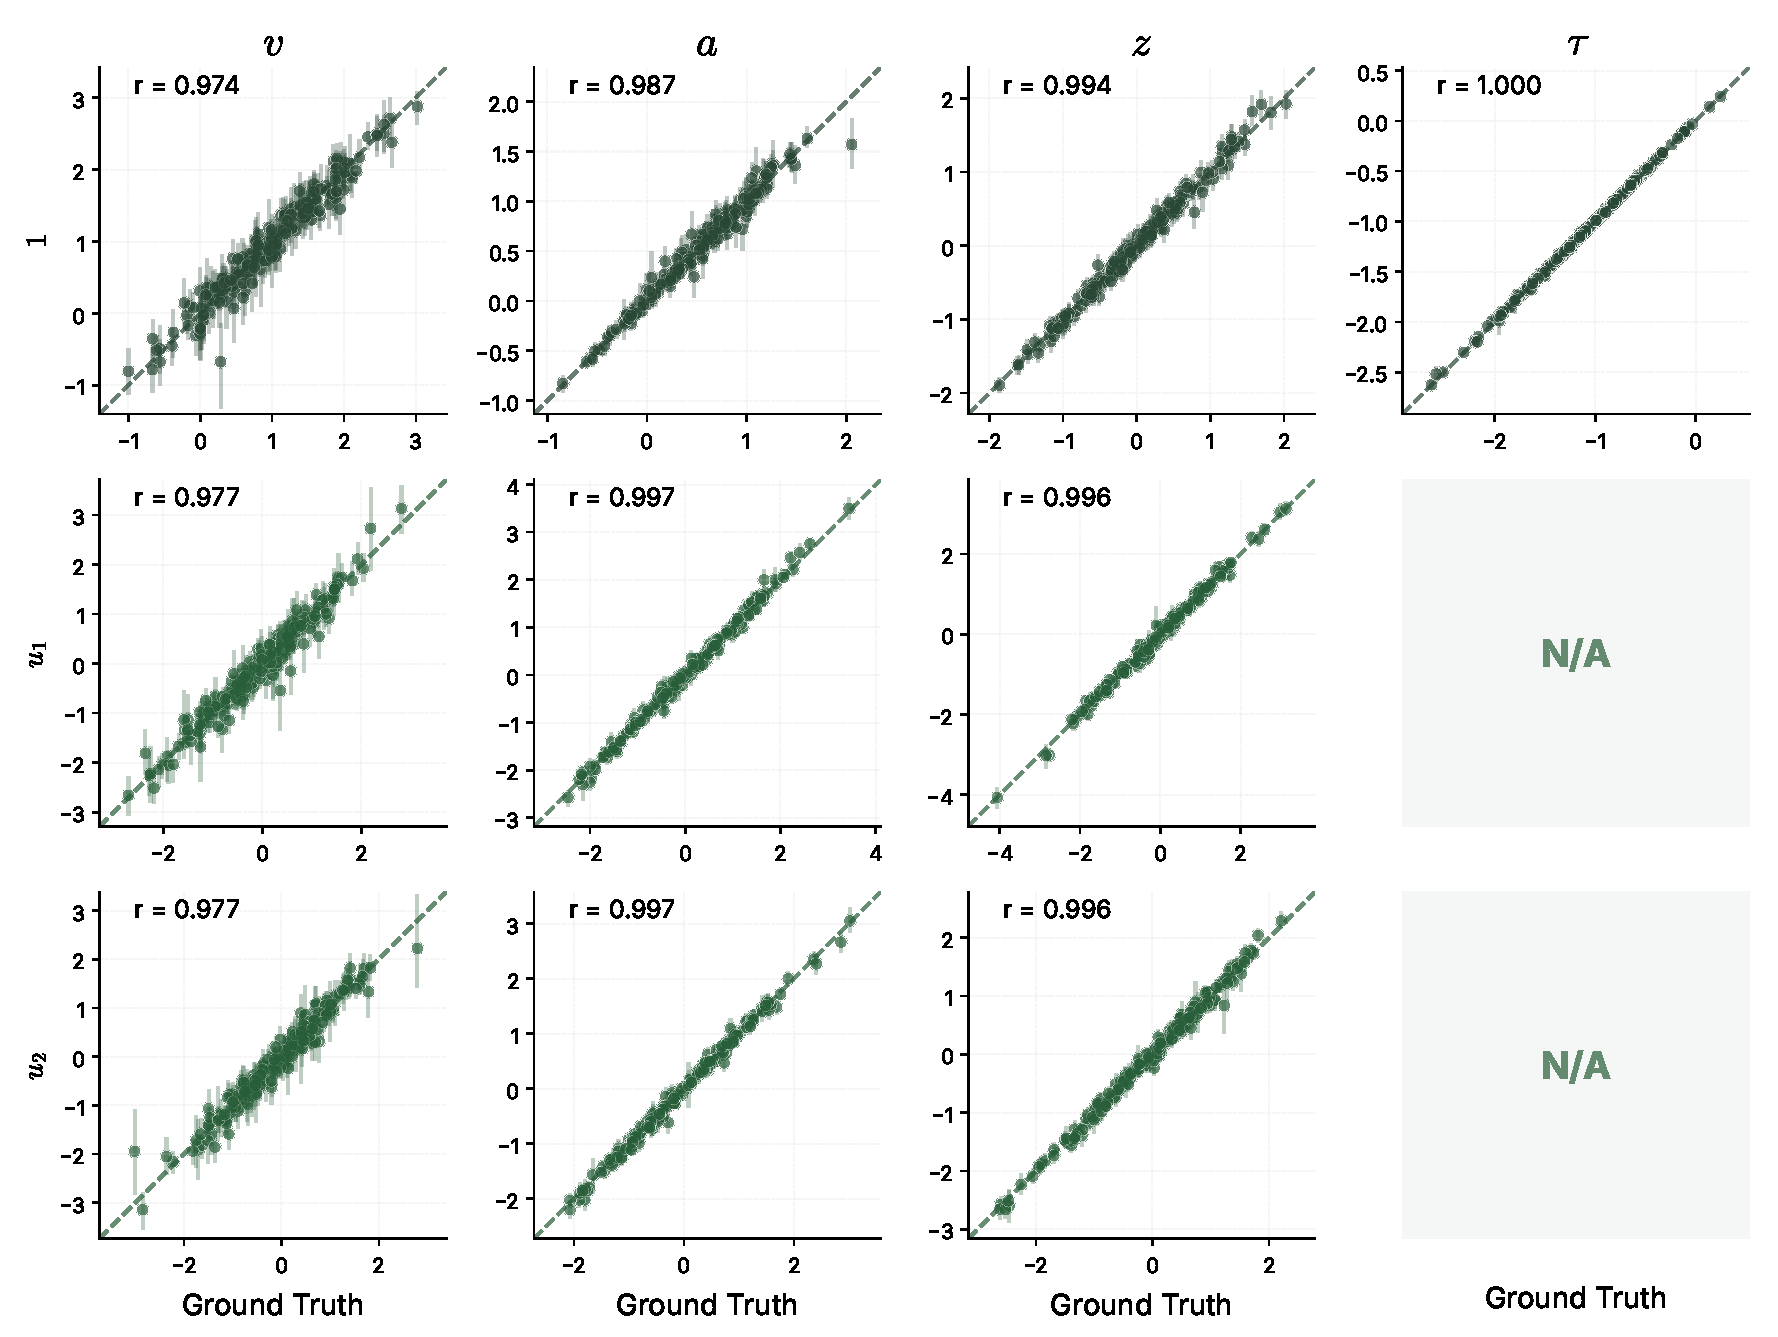
\includegraphics[width=\textwidth,height=0.3\textheight,keepaspectratio]{ddm/fixed_regressed/bf_recovery.pdf}\par\vspace{1ex}
  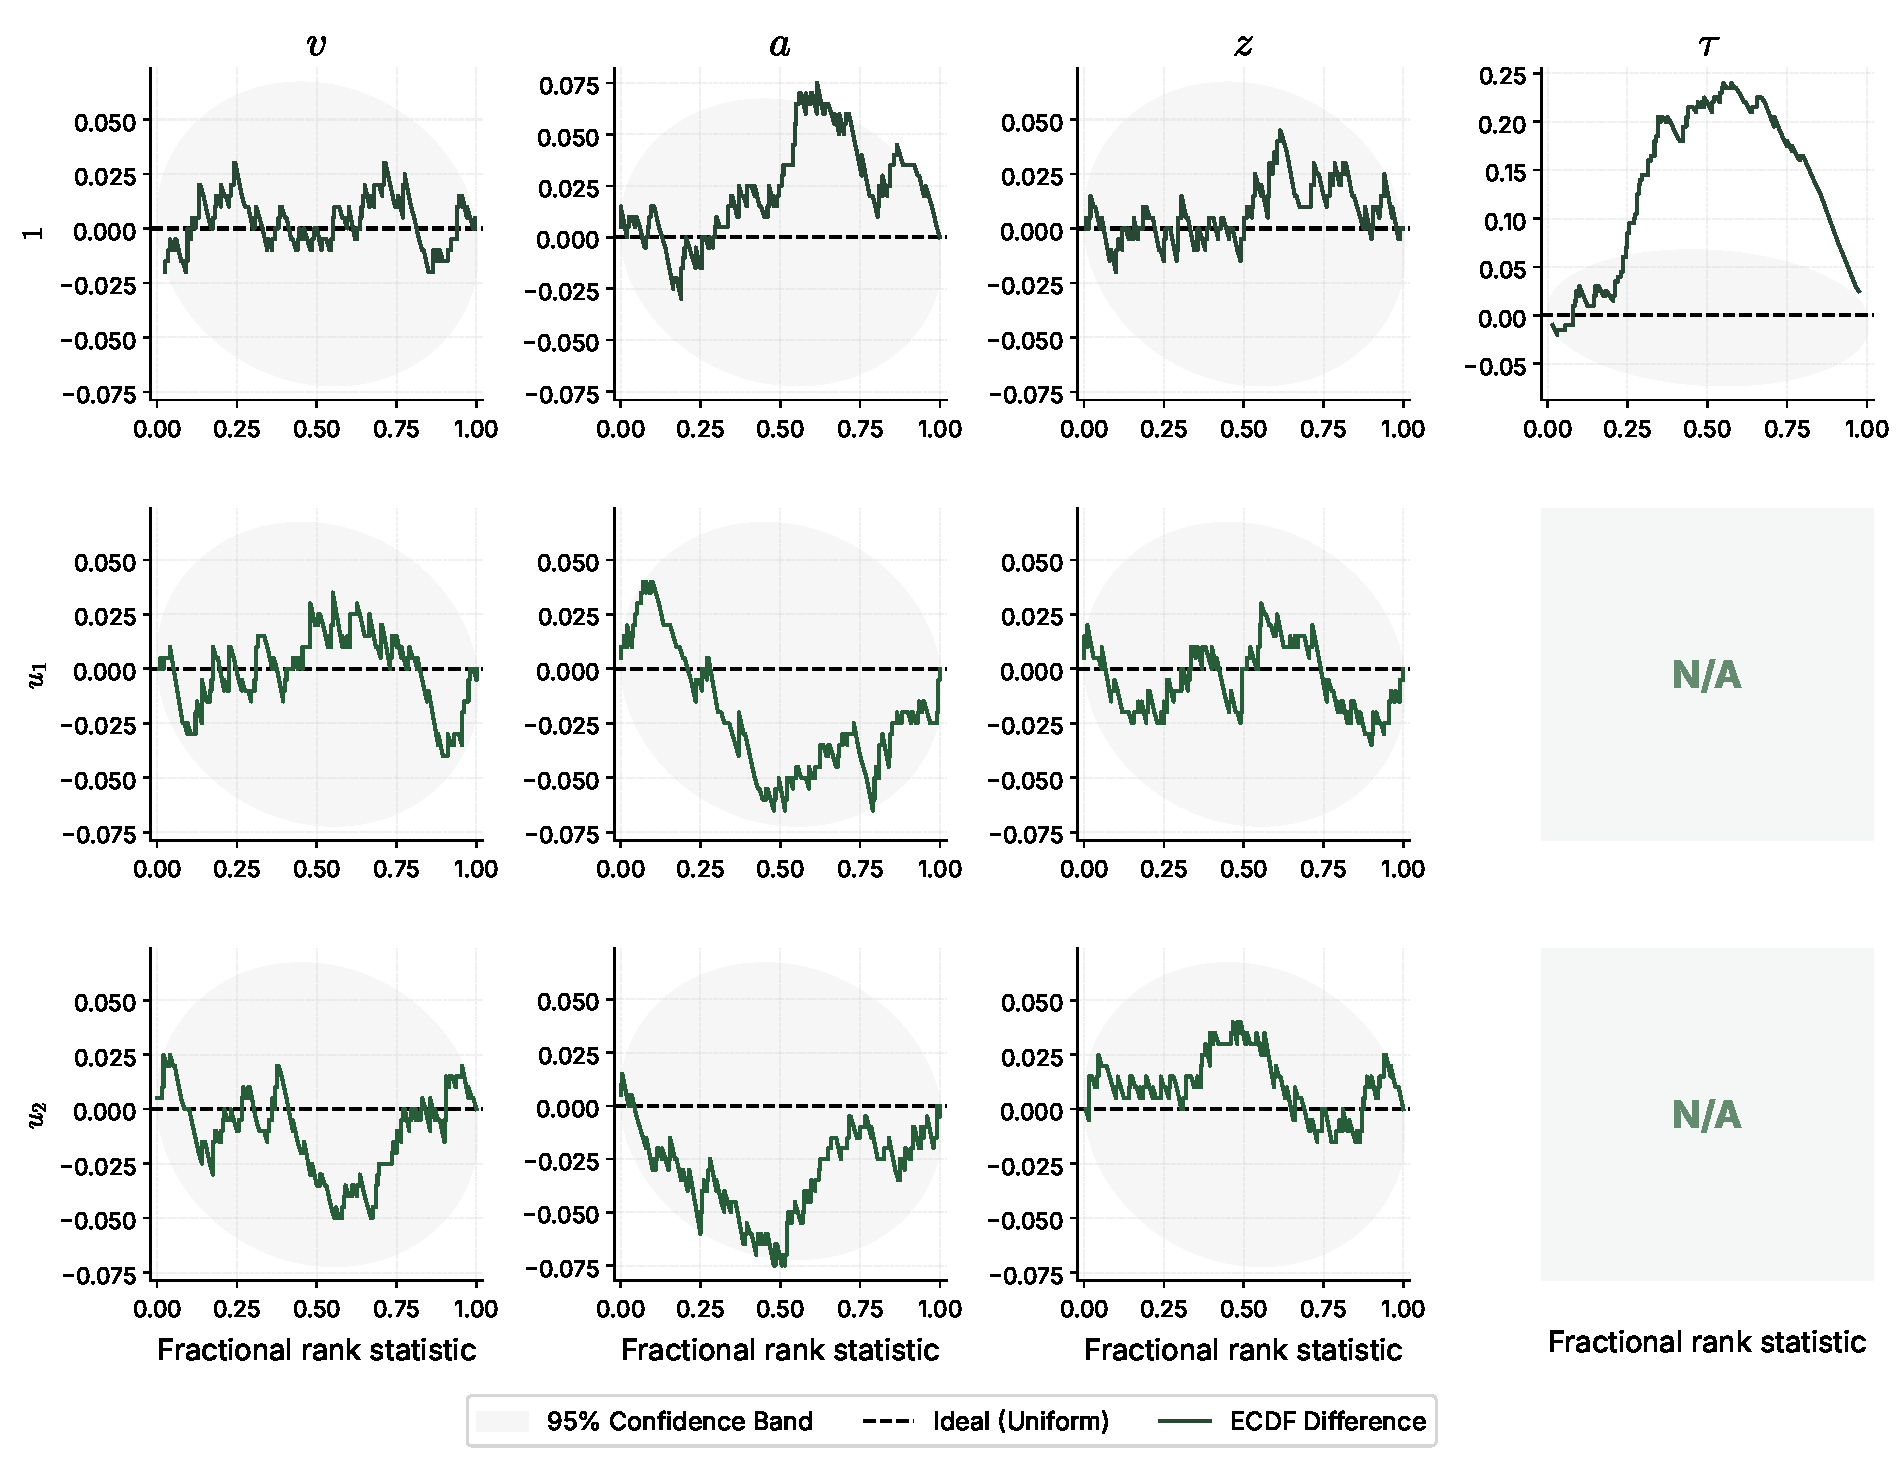
\includegraphics[width=\textwidth,height=0.3\textheight,keepaspectratio]{ddm/fixed_regressed/bf_ecdf.pdf}\par\vspace{1ex}
  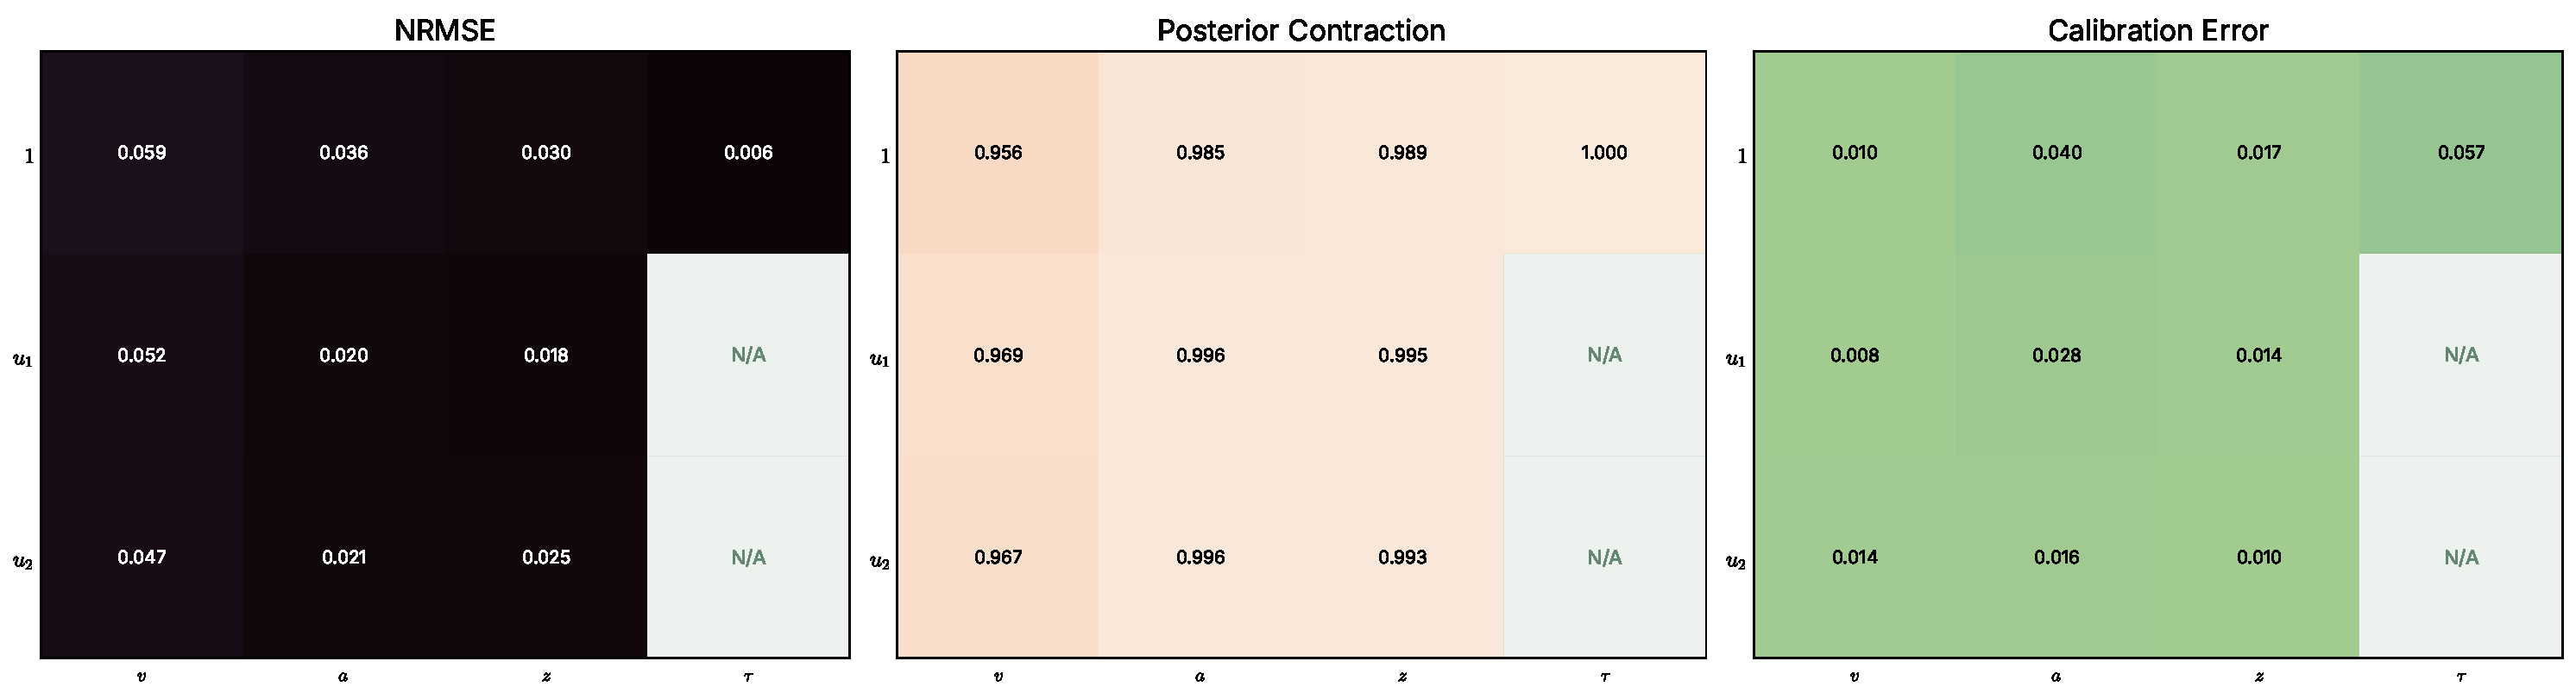
\includegraphics[width=\textwidth]{ddm/fixed_regressed/bf_metrics.pdf}
  \caption{\textbf{DDM, \emph{fixed + regressed} design: BayesFlow baseline.} Recovery (top), calibration (middle), metrics (bottom). $s_v$ and $s_\tau$ are fixed at 0 and not estimated; $v$, $a$ and $z$ carry slopes on $u_1$ and $u_2$ (10 coefficients shown). Layout and encoding as in Figure~\ref{fig:app1-ddm-intercept-only-cf}.}
  \label{fig:app1-ddm-fixed-regressed-bf}
\end{figure}

\begin{figure}[p]
  \centering
  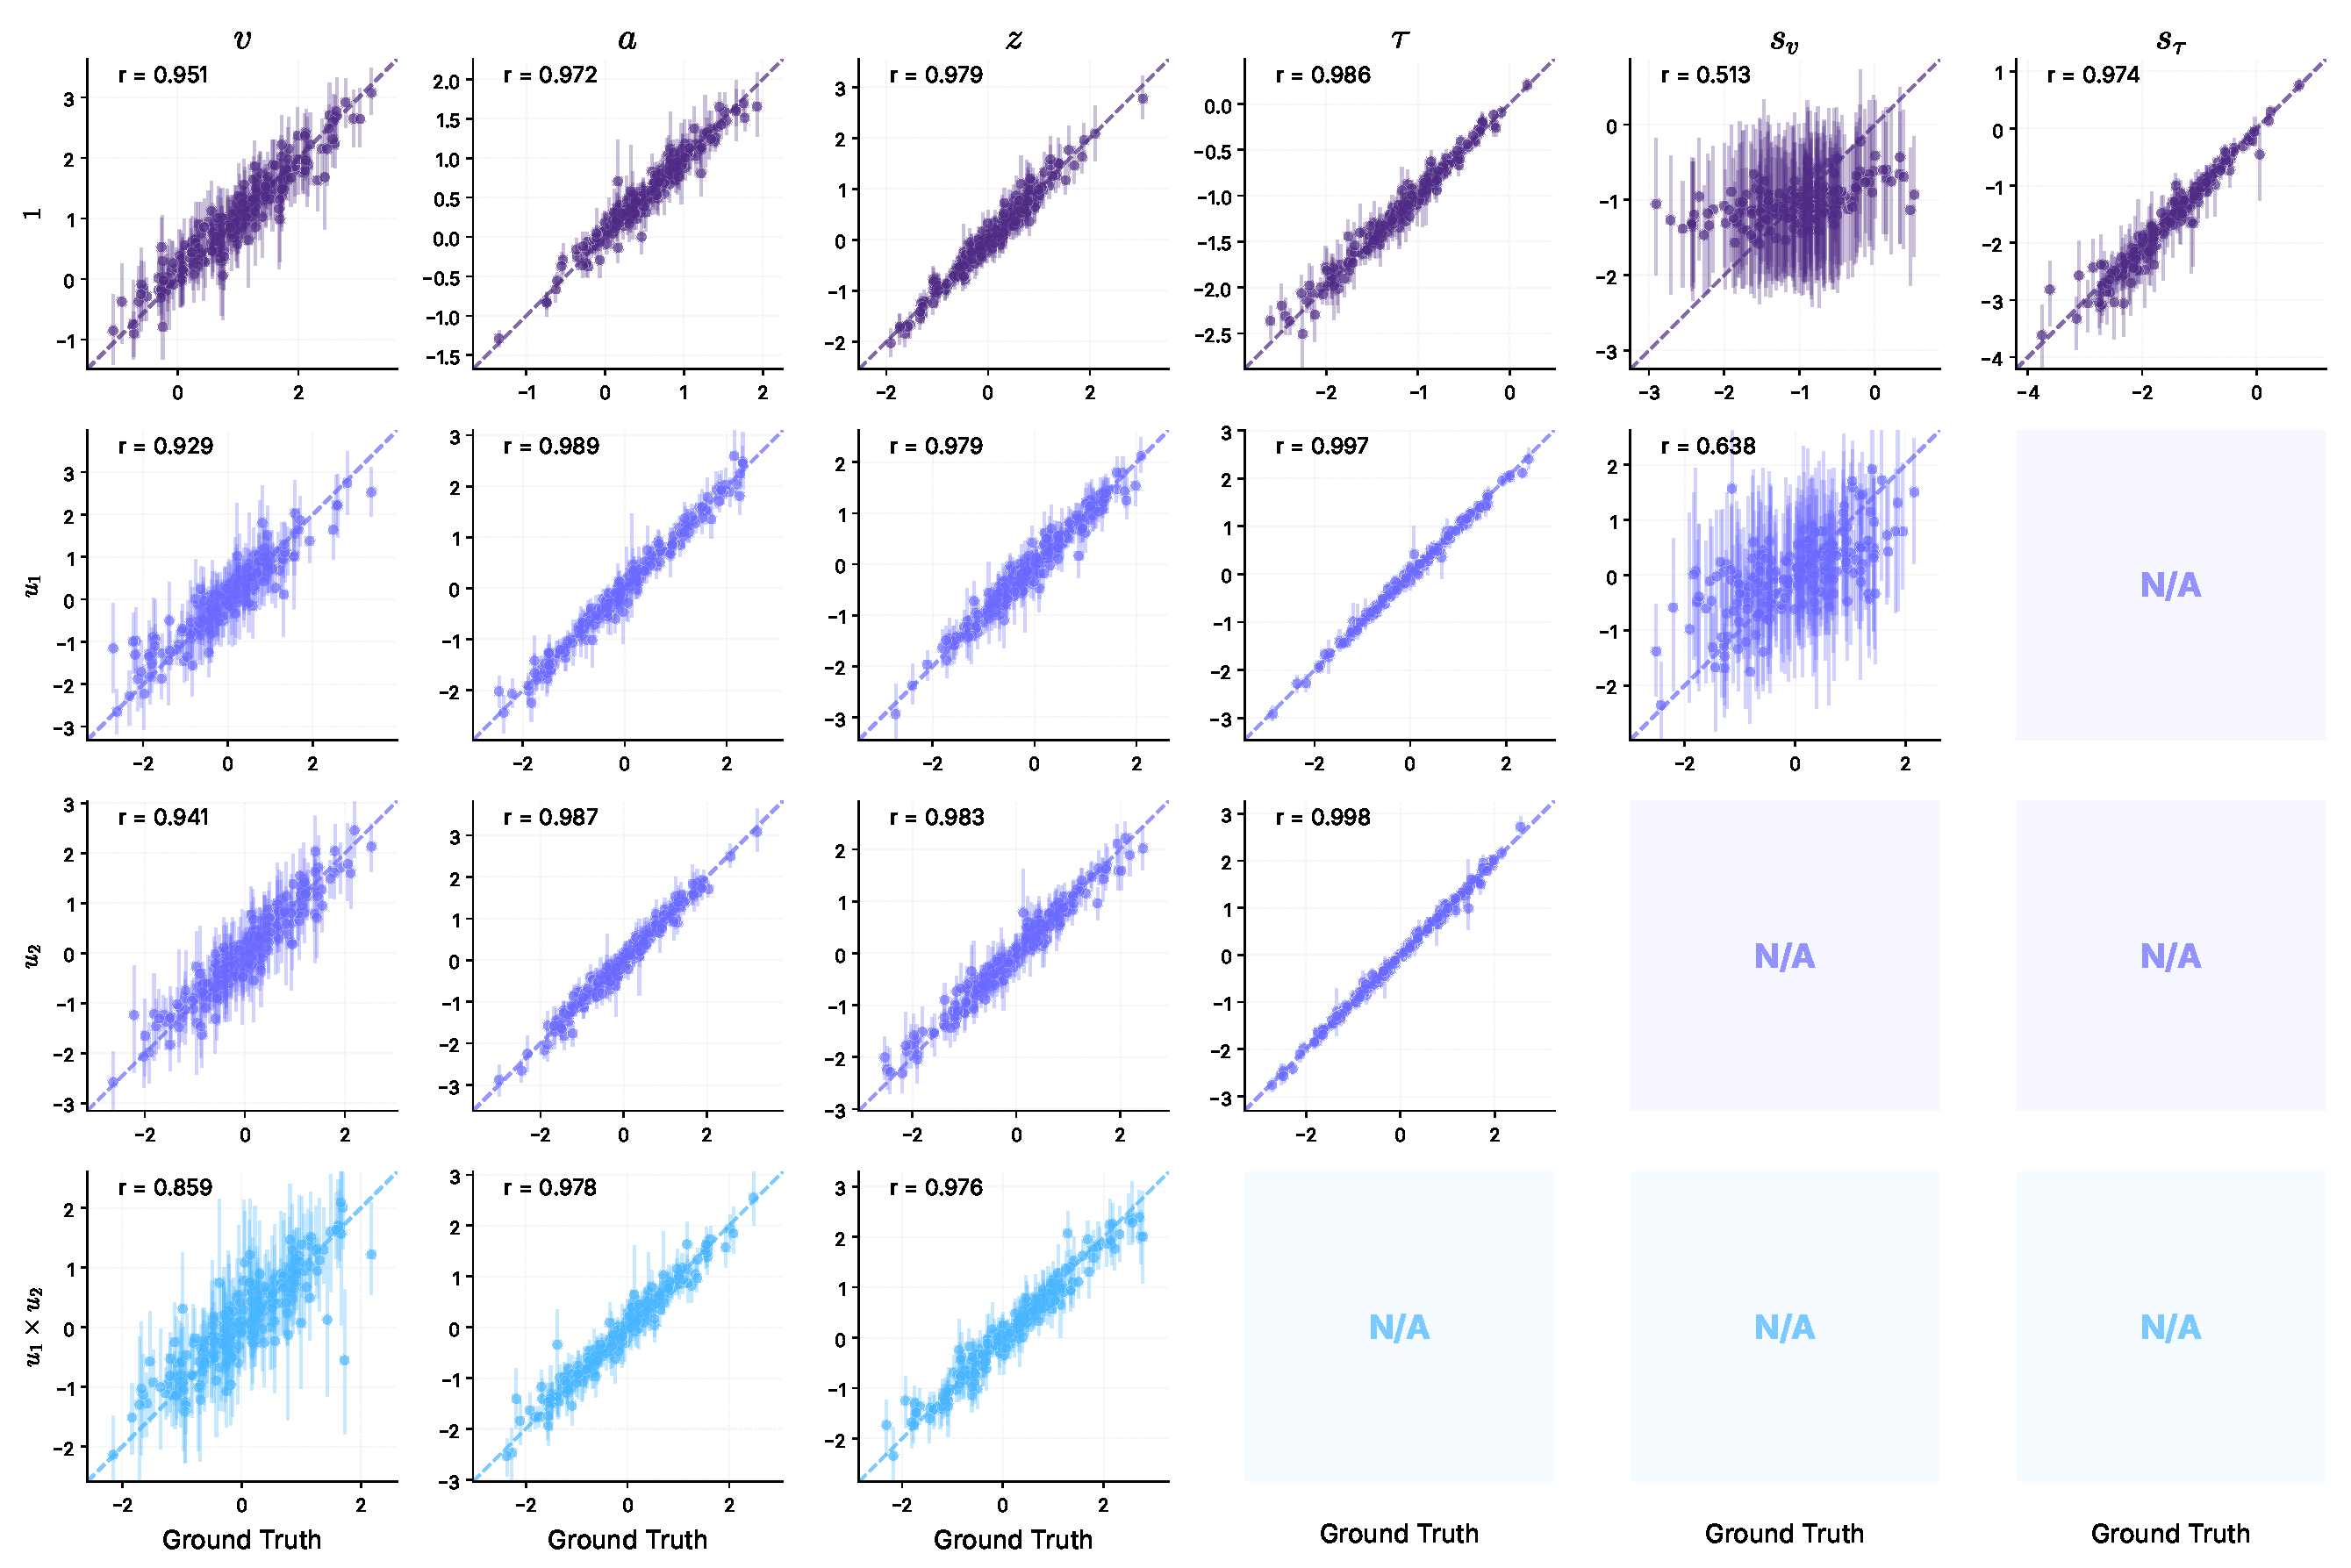
\includegraphics[width=\textwidth,height=0.3\textheight,keepaspectratio]{ddm/interaction/cf_recovery.pdf}\par\vspace{1ex}
  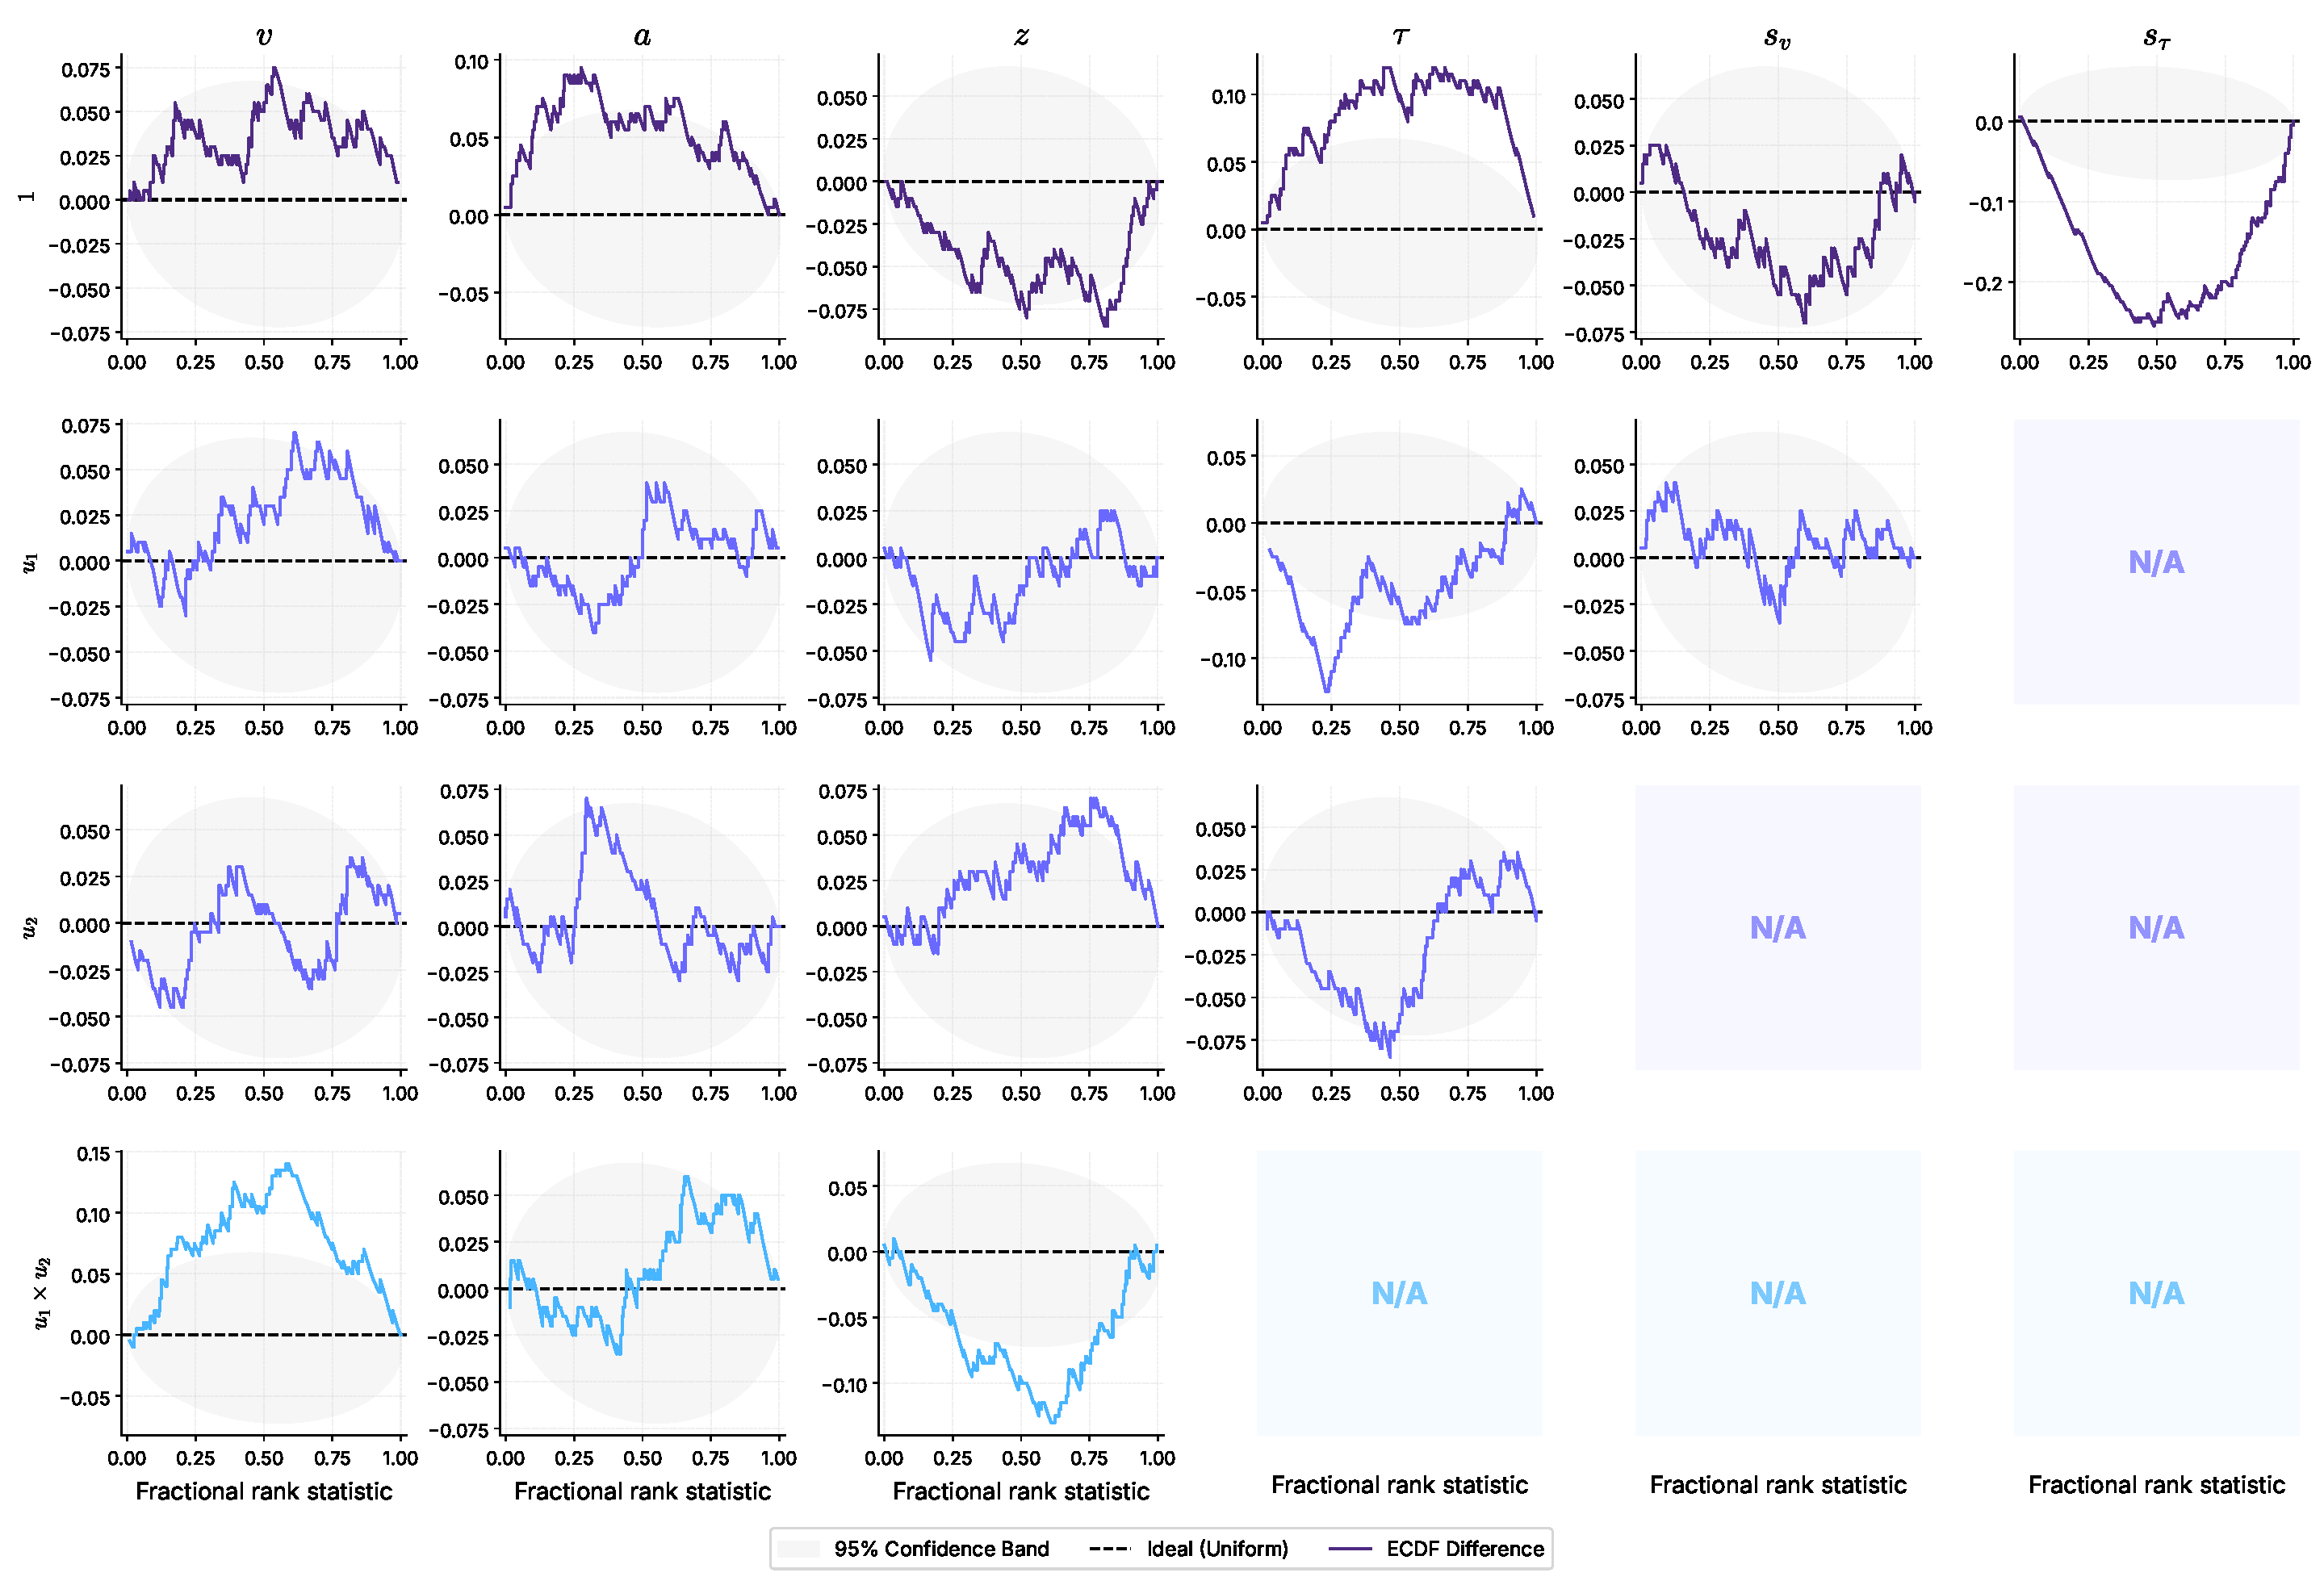
\includegraphics[width=\textwidth,height=0.3\textheight,keepaspectratio]{ddm/interaction/cf_ecdf.pdf}\par\vspace{1ex}
  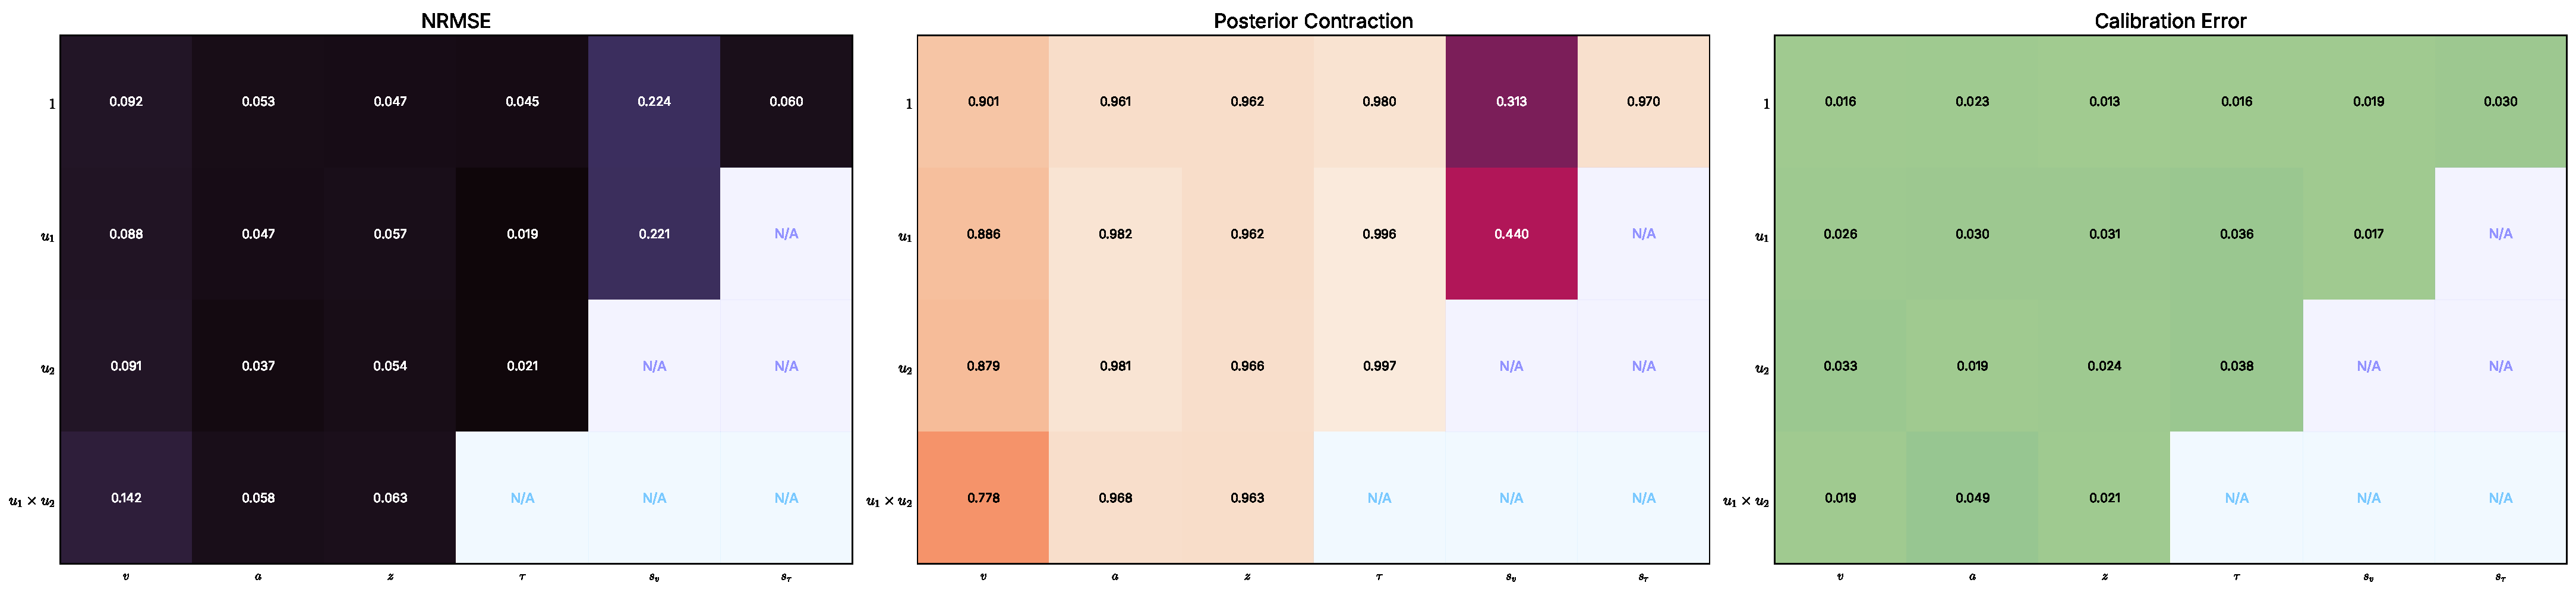
\includegraphics[width=\textwidth]{ddm/interaction/cf_metrics.pdf}
  \caption{\textbf{DDM, \emph{interaction} design: CogFormer.} Recovery (top), calibration (middle), metrics (bottom). $v$, $a$, $z$, $\tau$ and $s_v$ carry slopes on $u_1$; $v$, $a$, $z$ and $\tau$ carry slopes on $u_2$; $v$, $a$ and $z$ on the product $u_1 u_2$ (18 coefficients shown). Layout and encoding as in Figure~\ref{fig:app1-ddm-intercept-only-cf}.}
  \label{fig:app1-ddm-interaction-cf}
\end{figure}

\begin{figure}[p]
  \centering
  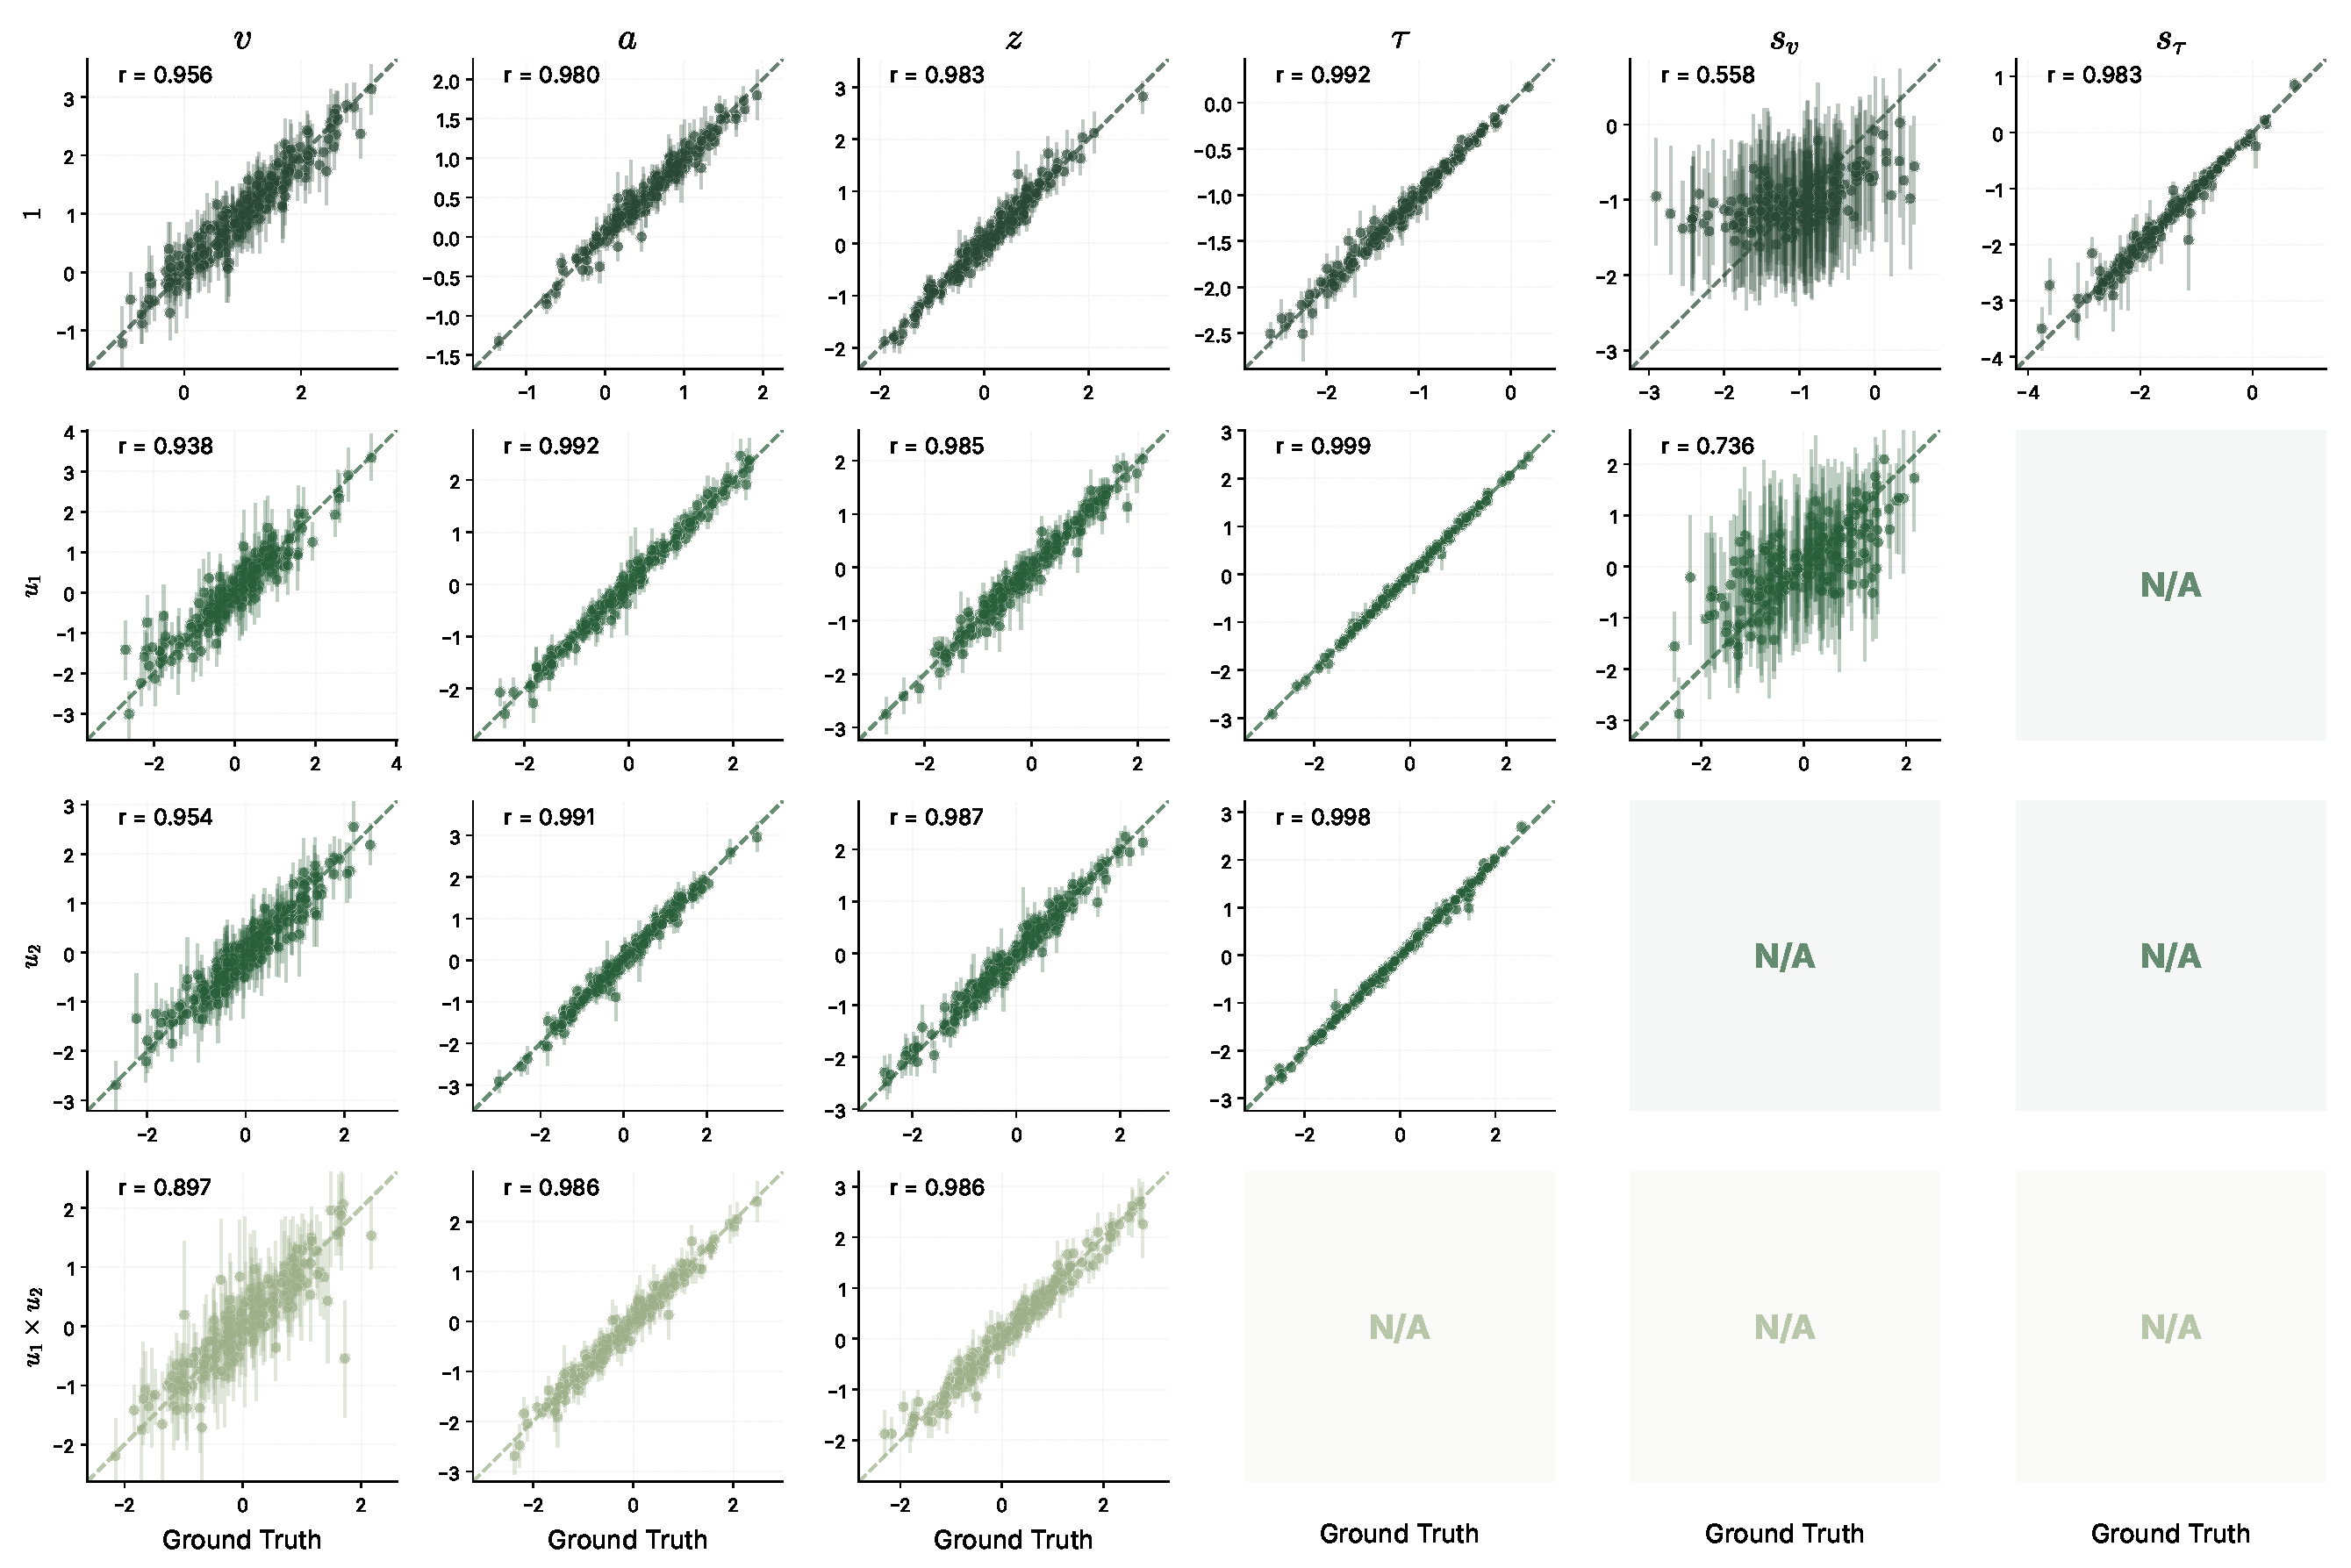
\includegraphics[width=\textwidth,height=0.3\textheight,keepaspectratio]{ddm/interaction/bf_recovery.pdf}\par\vspace{1ex}
  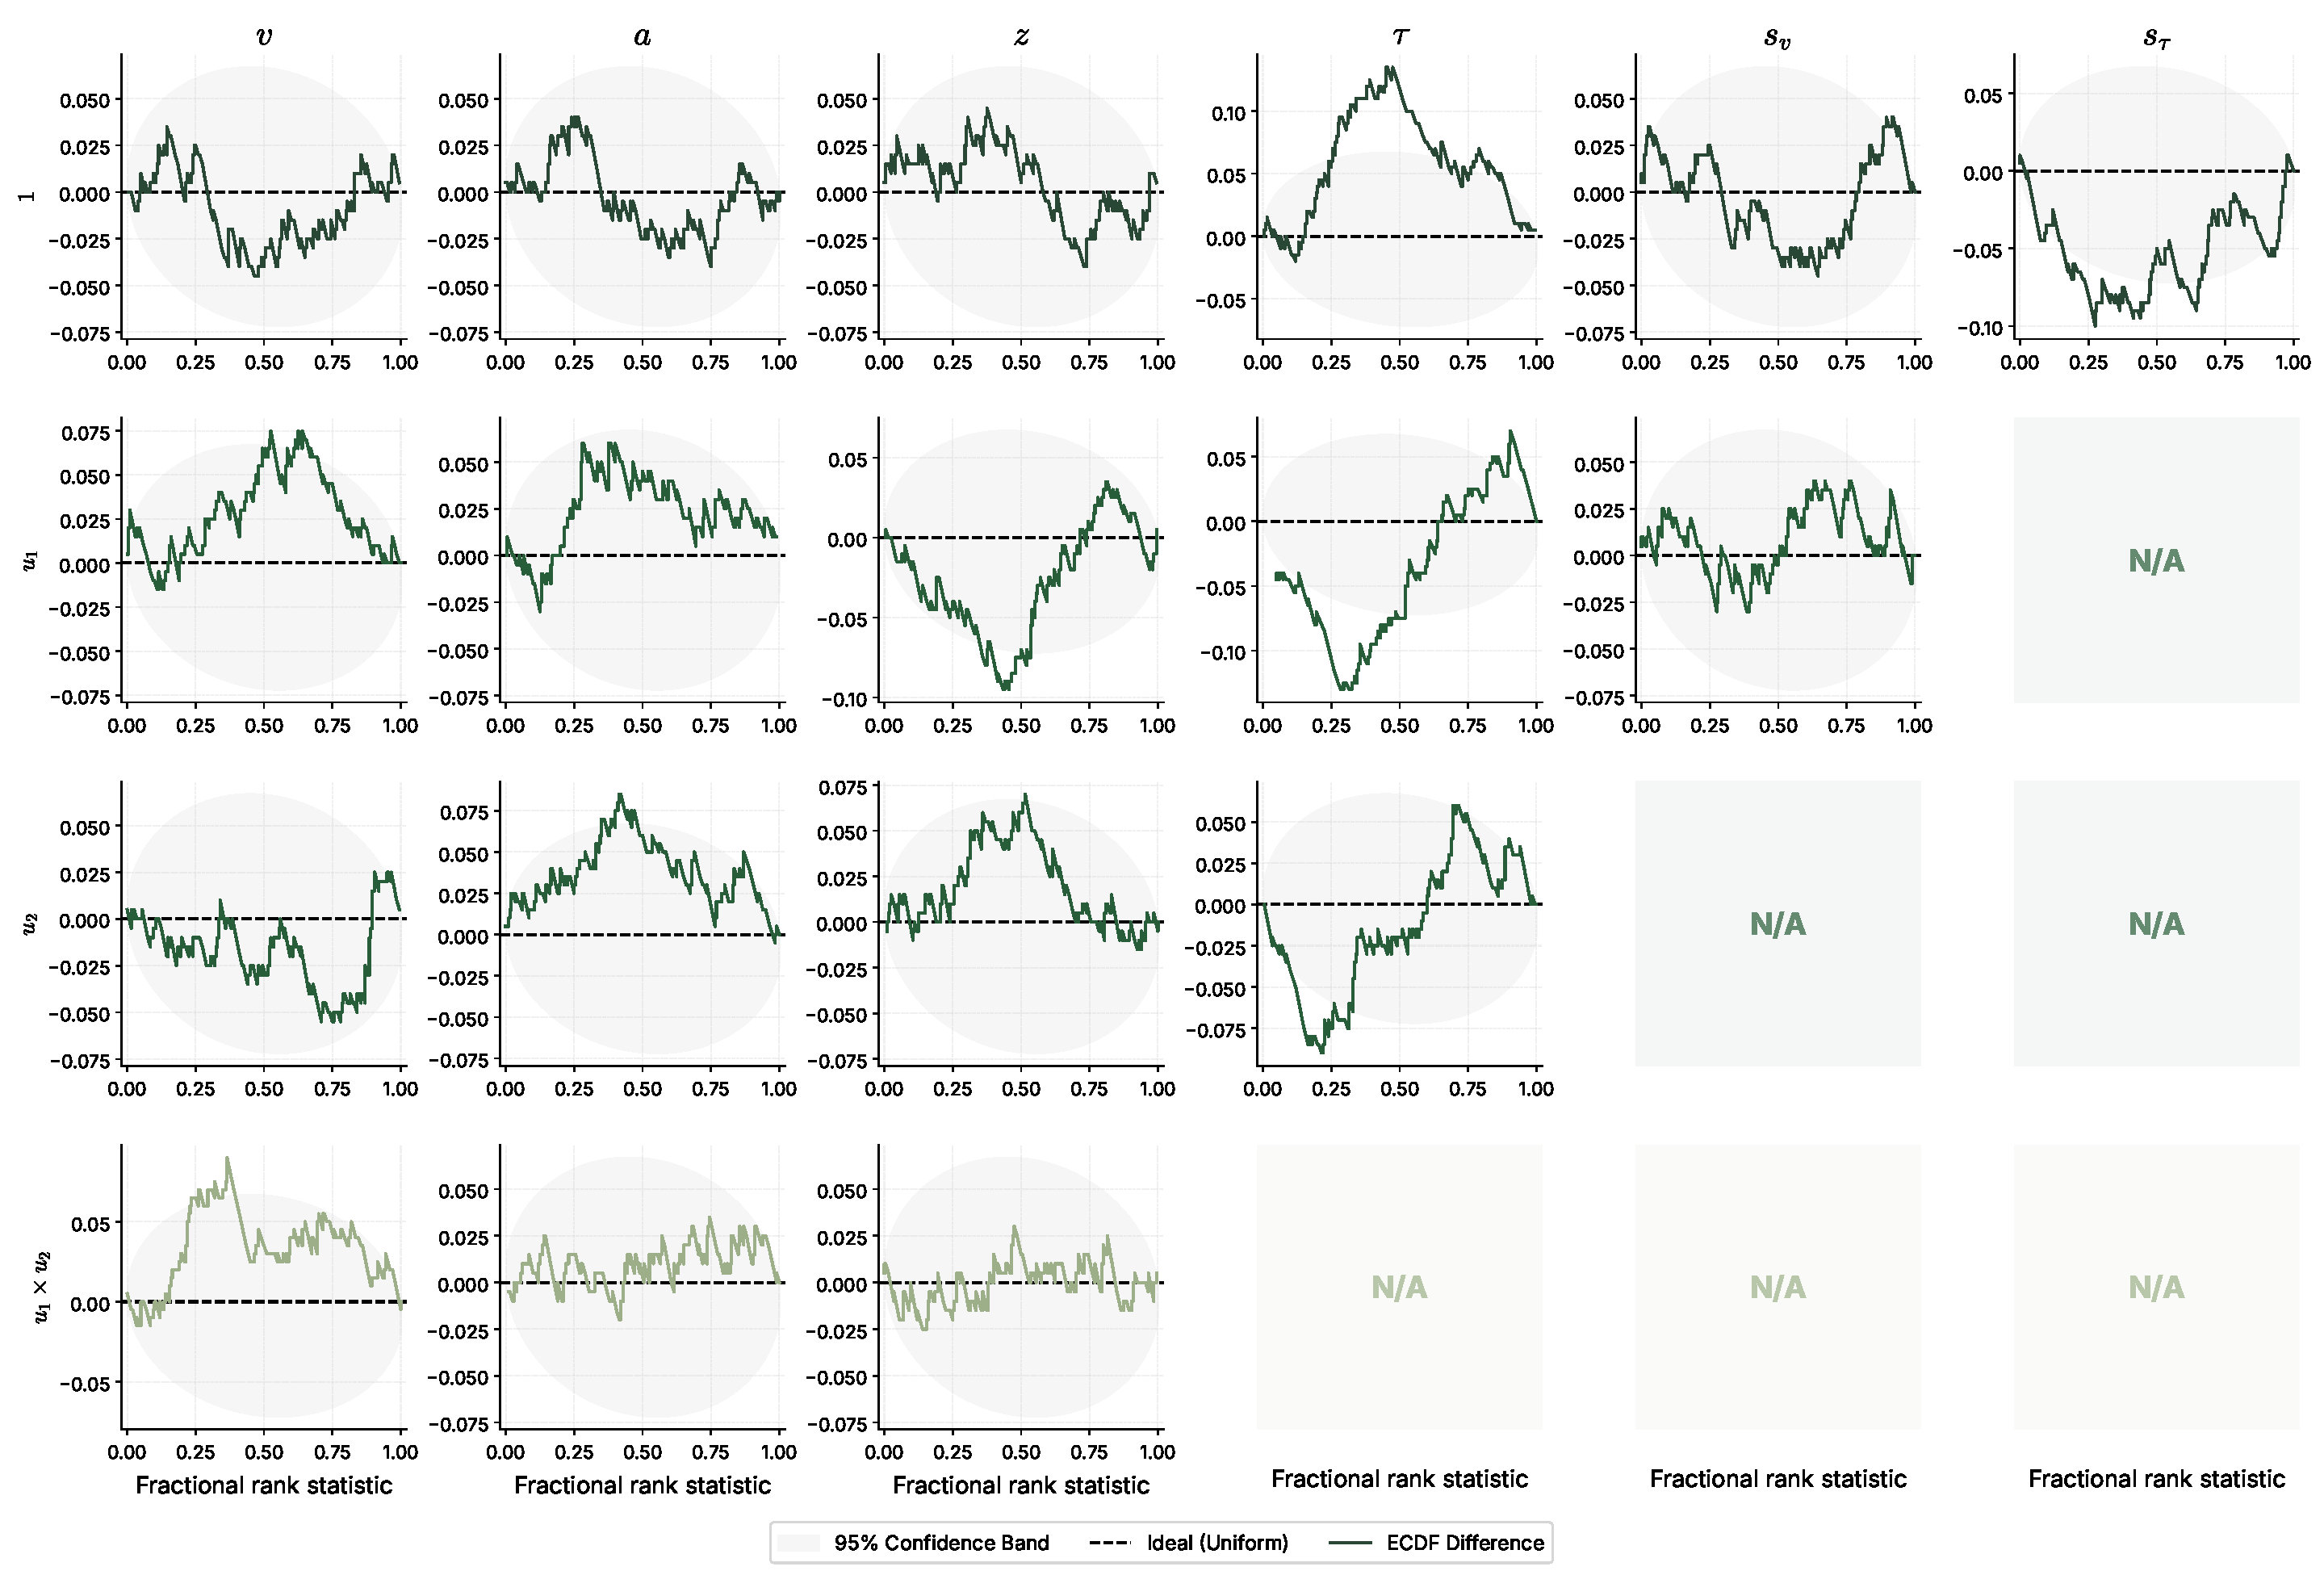
\includegraphics[width=\textwidth,height=0.3\textheight,keepaspectratio]{ddm/interaction/bf_ecdf.pdf}\par\vspace{1ex}
  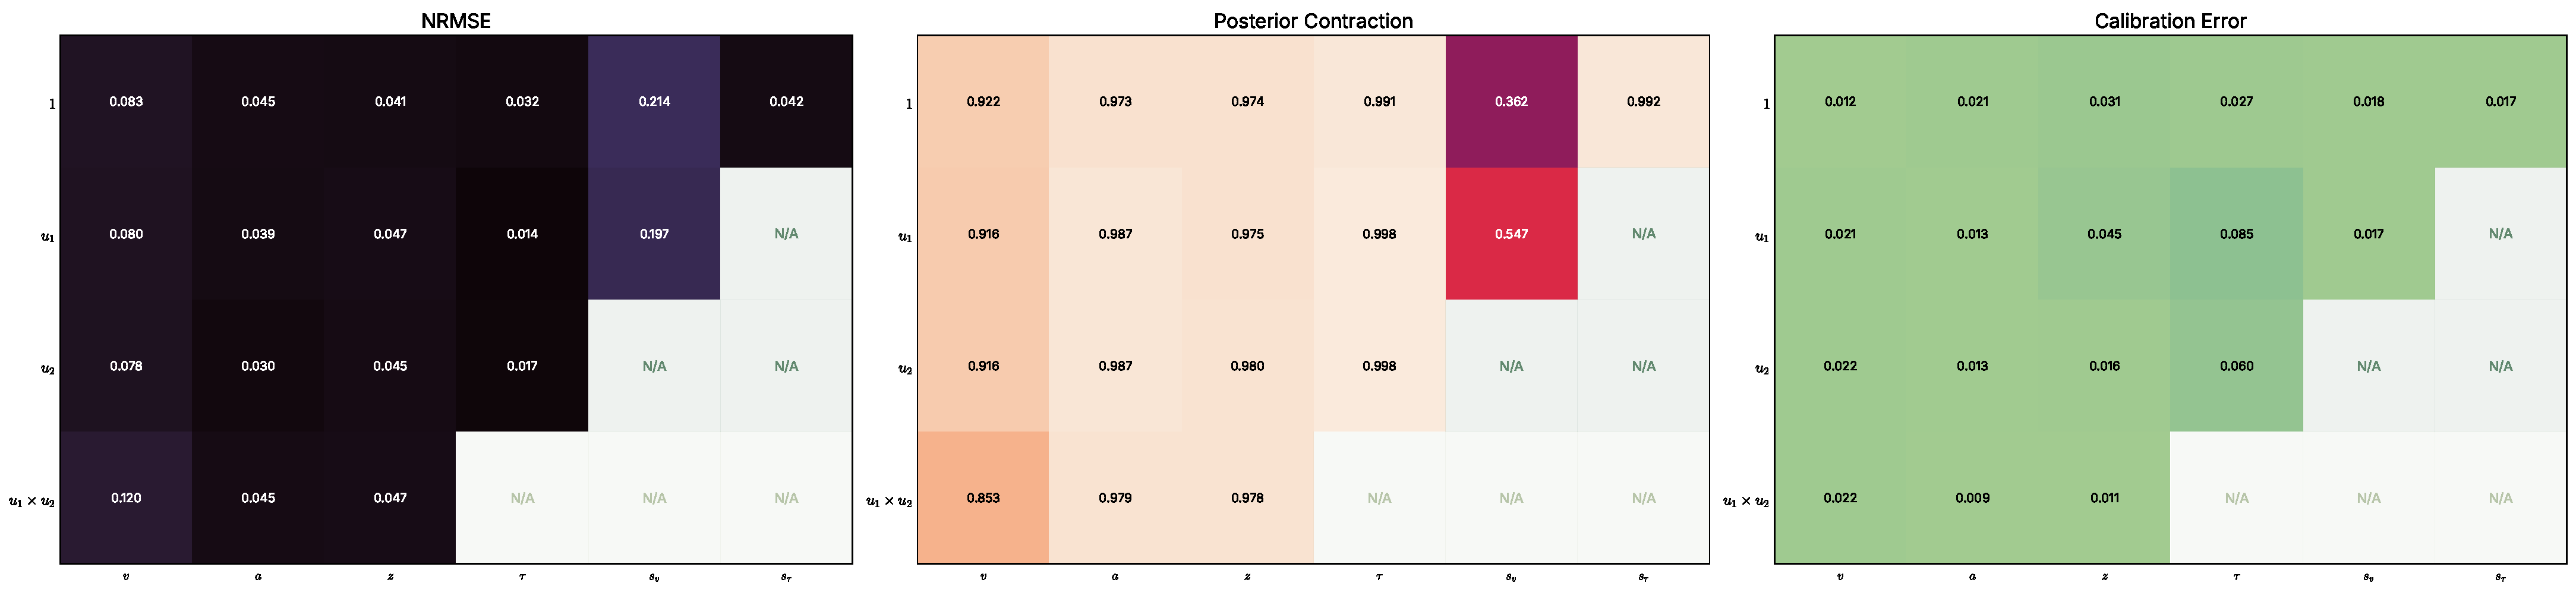
\includegraphics[width=\textwidth]{ddm/interaction/bf_metrics.pdf}
  \caption{\textbf{DDM, \emph{interaction} design: BayesFlow baseline.} Recovery (top), calibration (middle), metrics (bottom). $v$, $a$, $z$, $\tau$ and $s_v$ carry slopes on $u_1$; $v$, $a$, $z$ and $\tau$ carry slopes on $u_2$; $v$, $a$ and $z$ on the product $u_1 u_2$ (18 coefficients shown). Layout and encoding as in Figure~\ref{fig:app1-ddm-intercept-only-cf}.}
  \label{fig:app1-ddm-interaction-bf}
\end{figure}

\begin{figure}[p]
  \centering
  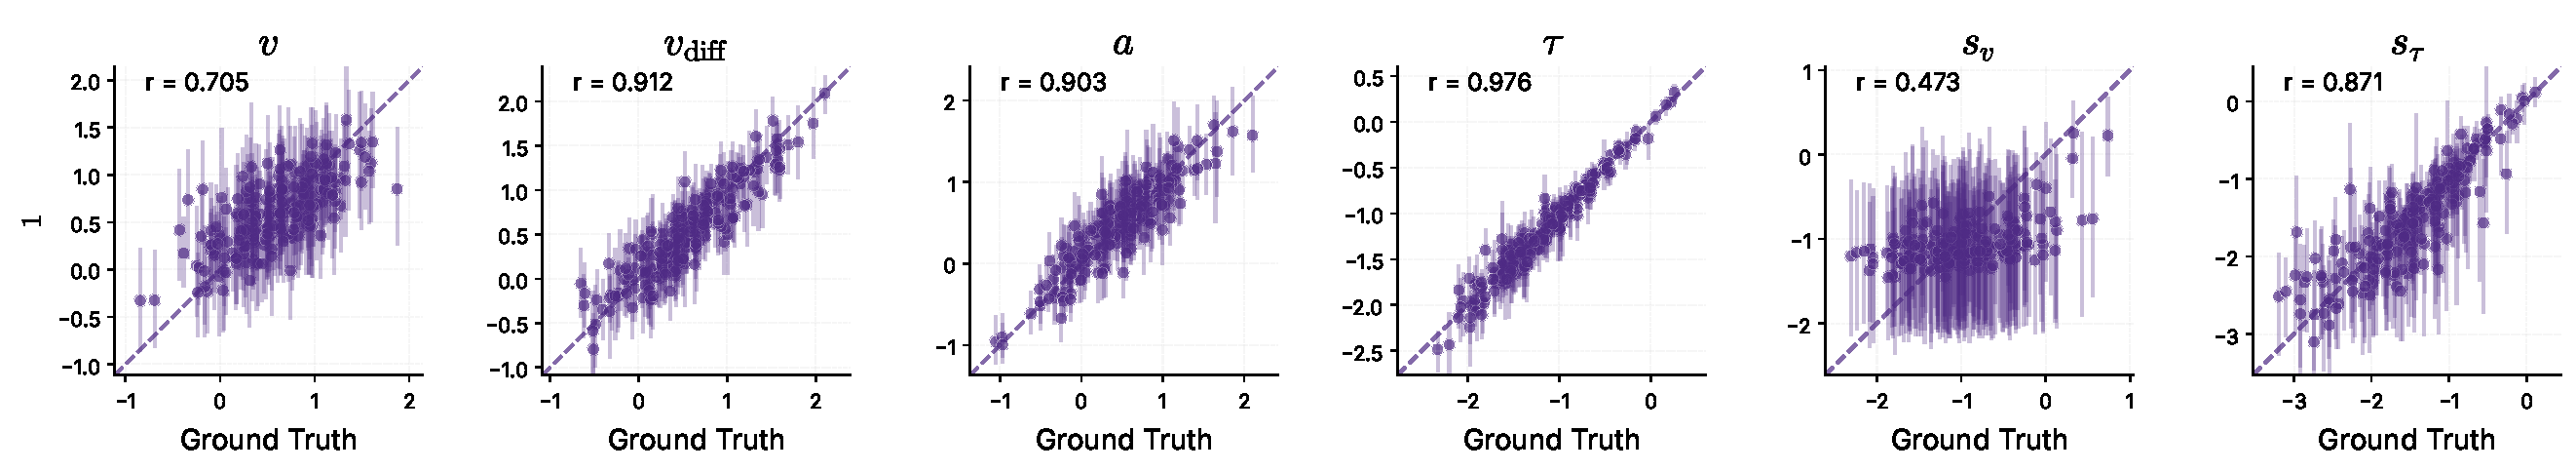
\includegraphics[width=\textwidth,height=0.3\textheight,keepaspectratio]{rdm/intercept_only/cf_recovery.pdf}\par\vspace{1ex}
  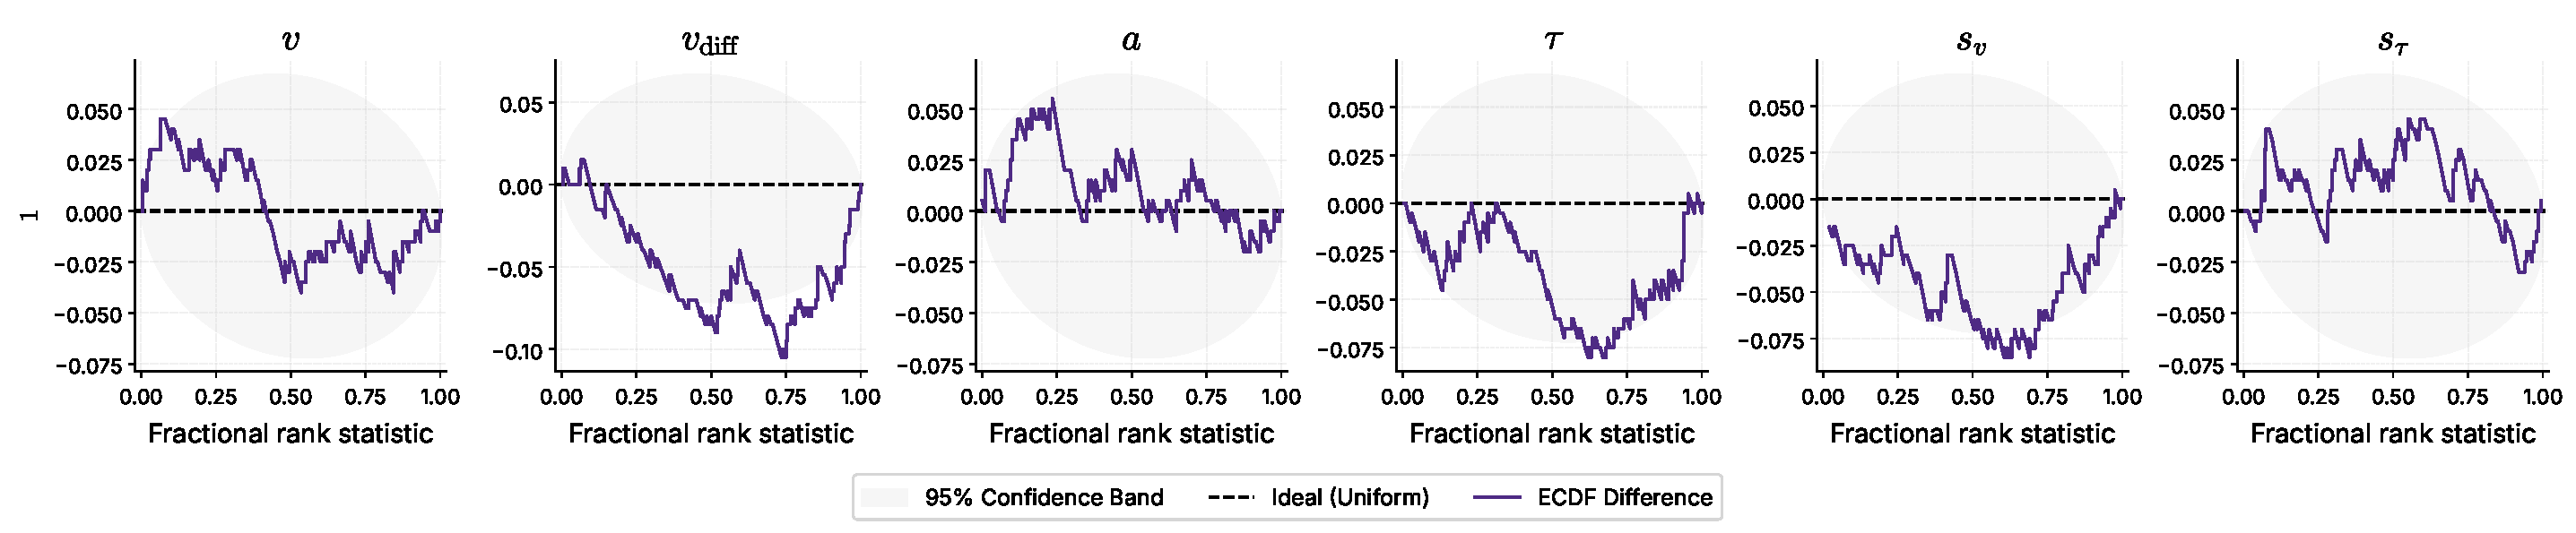
\includegraphics[width=\textwidth,height=0.3\textheight,keepaspectratio]{rdm/intercept_only/cf_ecdf.pdf}\par\vspace{1ex}
  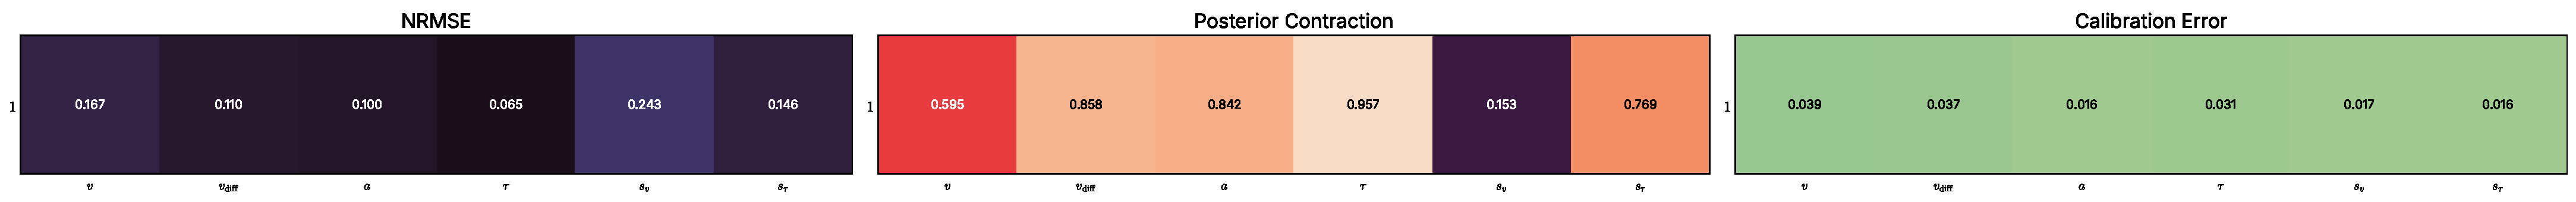
\includegraphics[width=\textwidth]{rdm/intercept_only/cf_metrics.pdf}
  \caption{\textbf{RDM, \emph{intercept-only} design: CogFormer.} Recovery (top), calibration (middle), metrics (bottom). Every estimated parameter enters as an intercept only (6 coefficients shown). Layout and encoding as in Figure~\ref{fig:app1-ddm-intercept-only-cf}.}
  \label{fig:app1-rdm-intercept-only-cf}
\end{figure}

\begin{figure}[p]
  \centering
  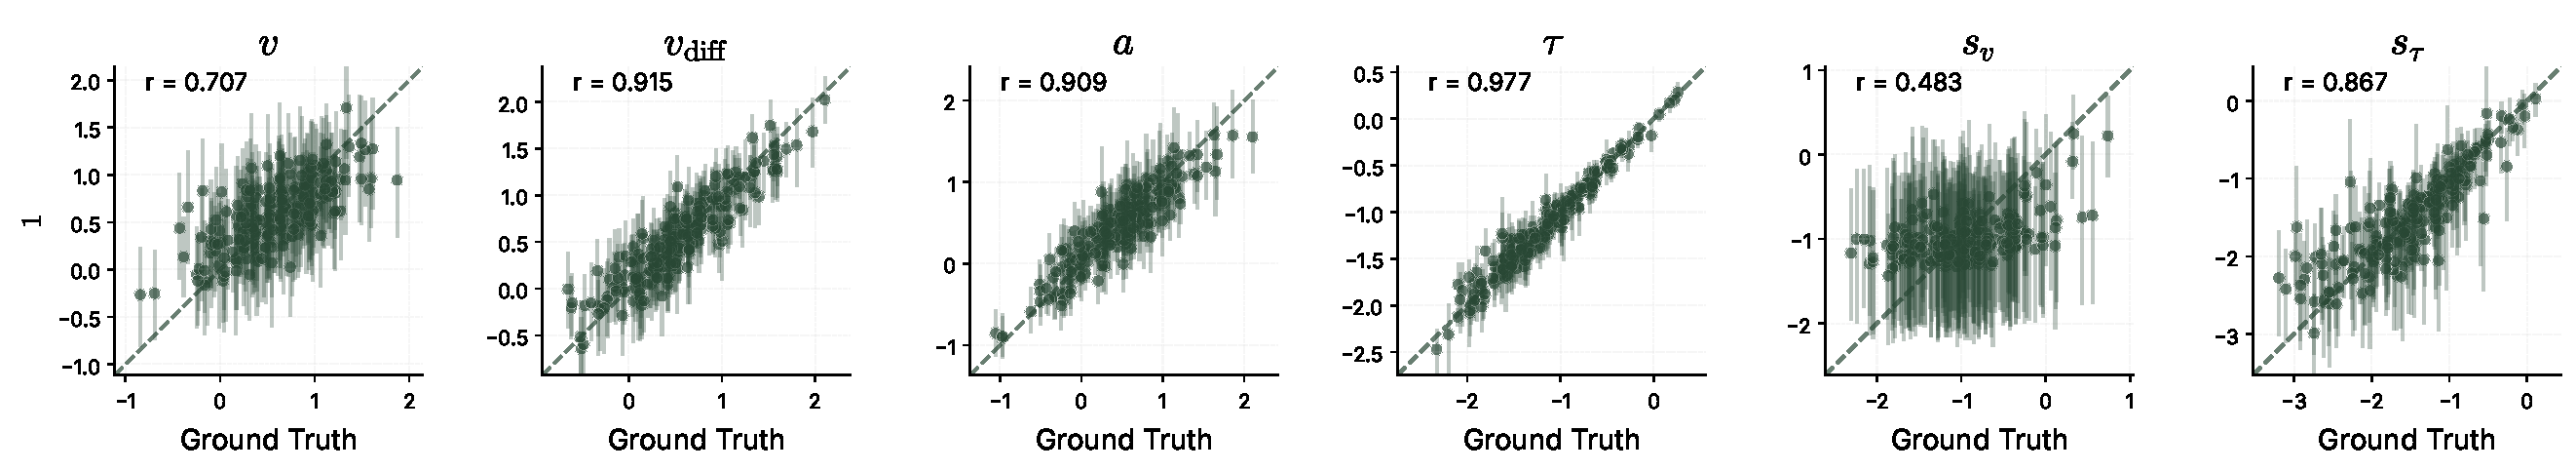
\includegraphics[width=\textwidth,height=0.3\textheight,keepaspectratio]{rdm/intercept_only/bf_recovery.pdf}\par\vspace{1ex}
  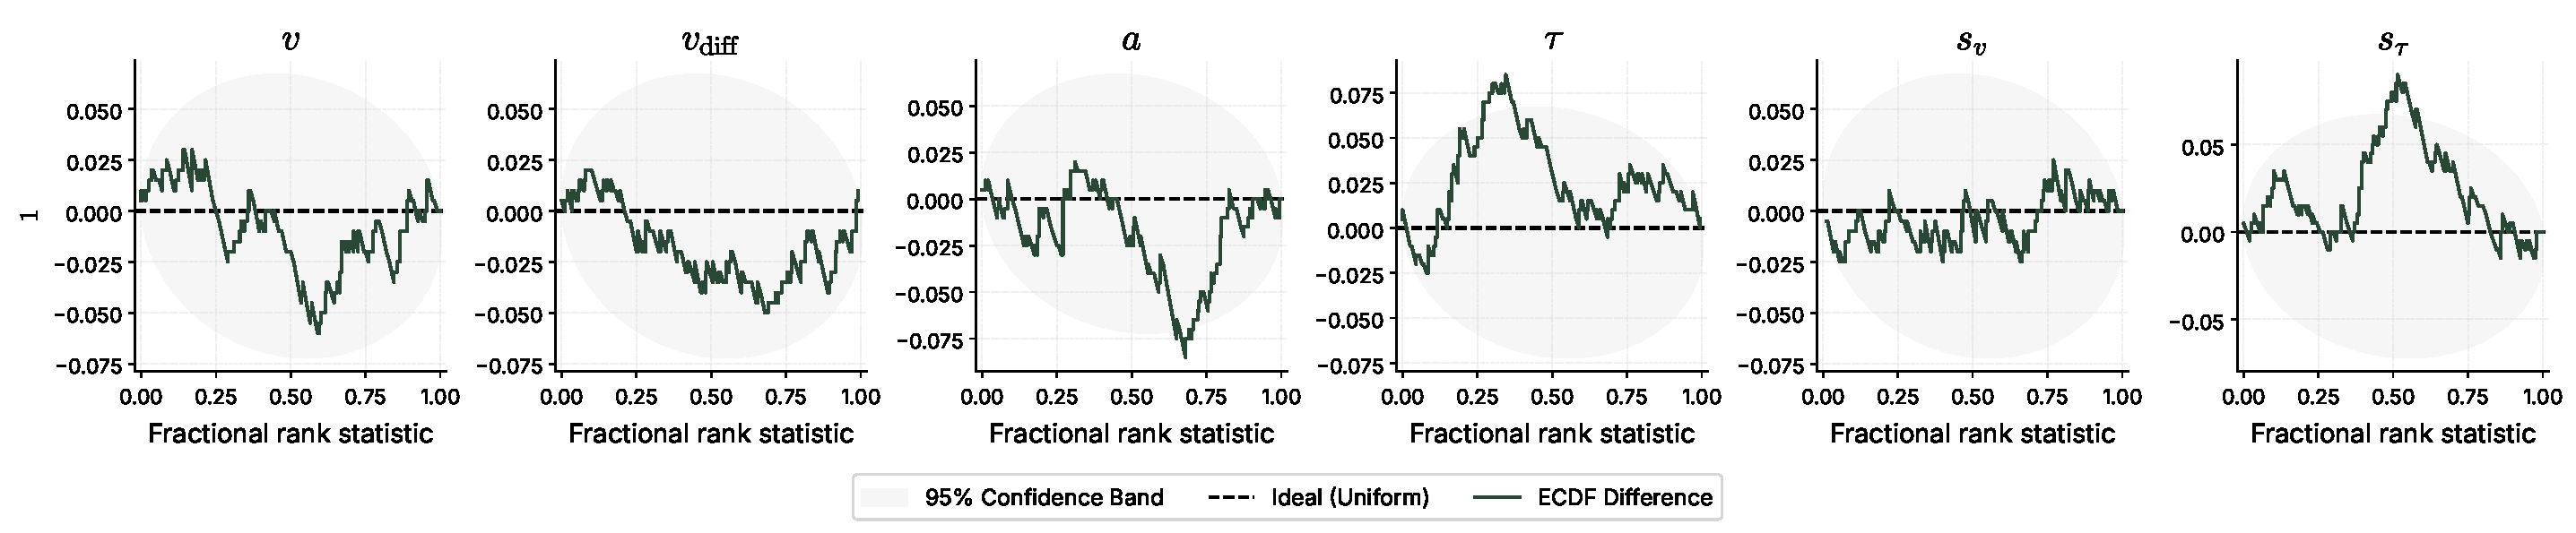
\includegraphics[width=\textwidth,height=0.3\textheight,keepaspectratio]{rdm/intercept_only/bf_ecdf.pdf}\par\vspace{1ex}
  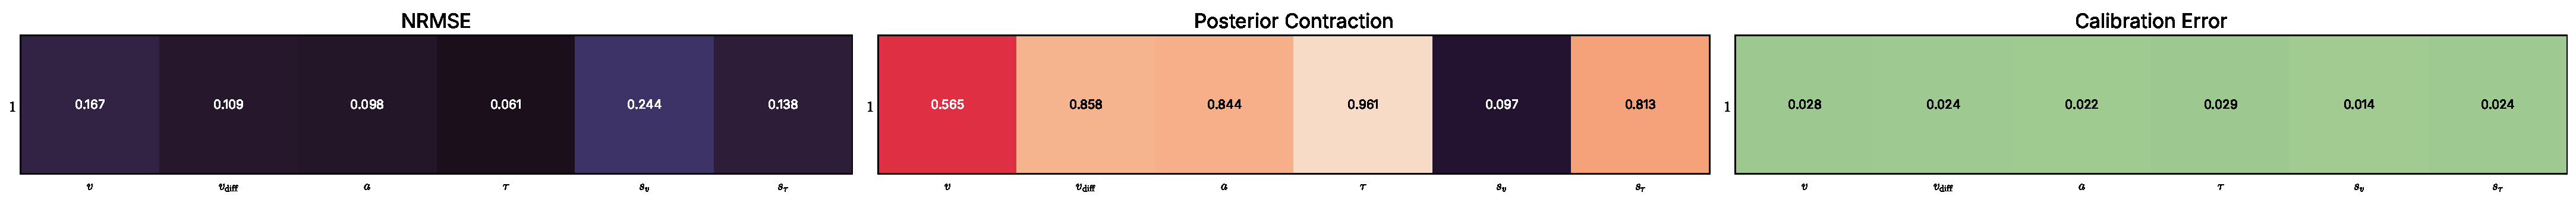
\includegraphics[width=\textwidth]{rdm/intercept_only/bf_metrics.pdf}
  \caption{\textbf{RDM, \emph{intercept-only} design: BayesFlow baseline.} Recovery (top), calibration (middle), metrics (bottom). Every estimated parameter enters as an intercept only (6 coefficients shown). Layout and encoding as in Figure~\ref{fig:app1-ddm-intercept-only-cf}.}
  \label{fig:app1-rdm-intercept-only-bf}
\end{figure}

\begin{figure}[p]
  \centering
  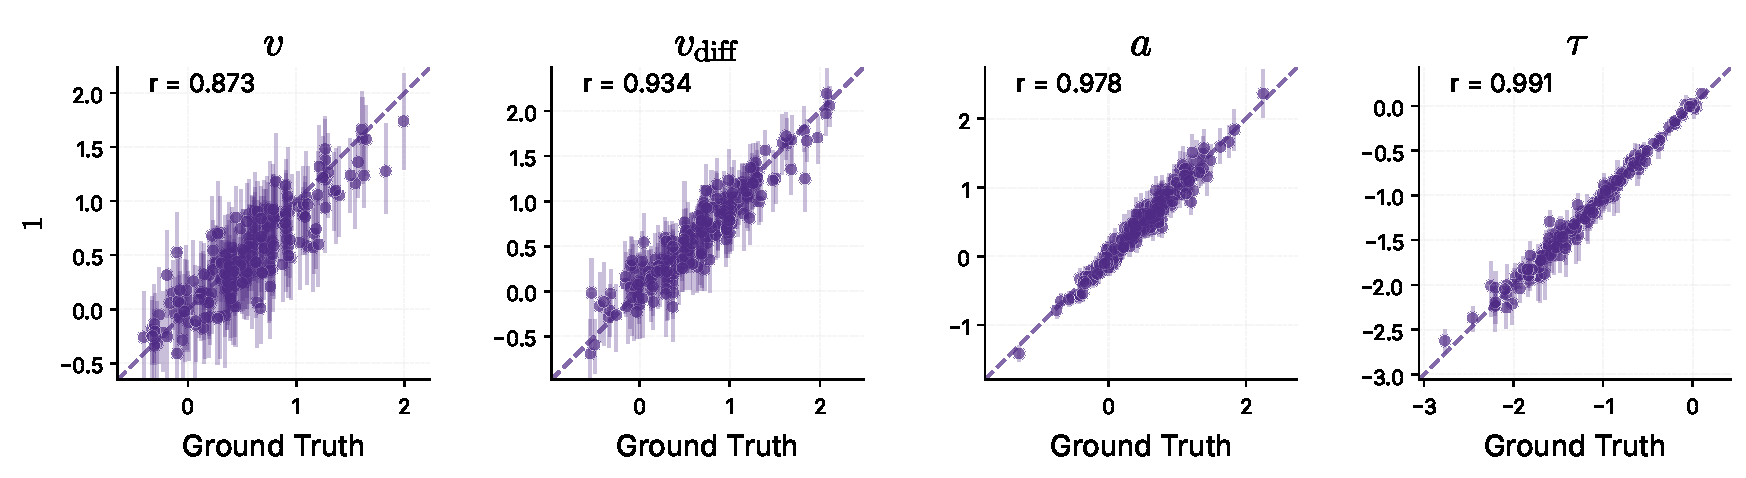
\includegraphics[width=\textwidth,height=0.3\textheight,keepaspectratio]{rdm/fixed/cf_recovery.pdf}\par\vspace{1ex}
  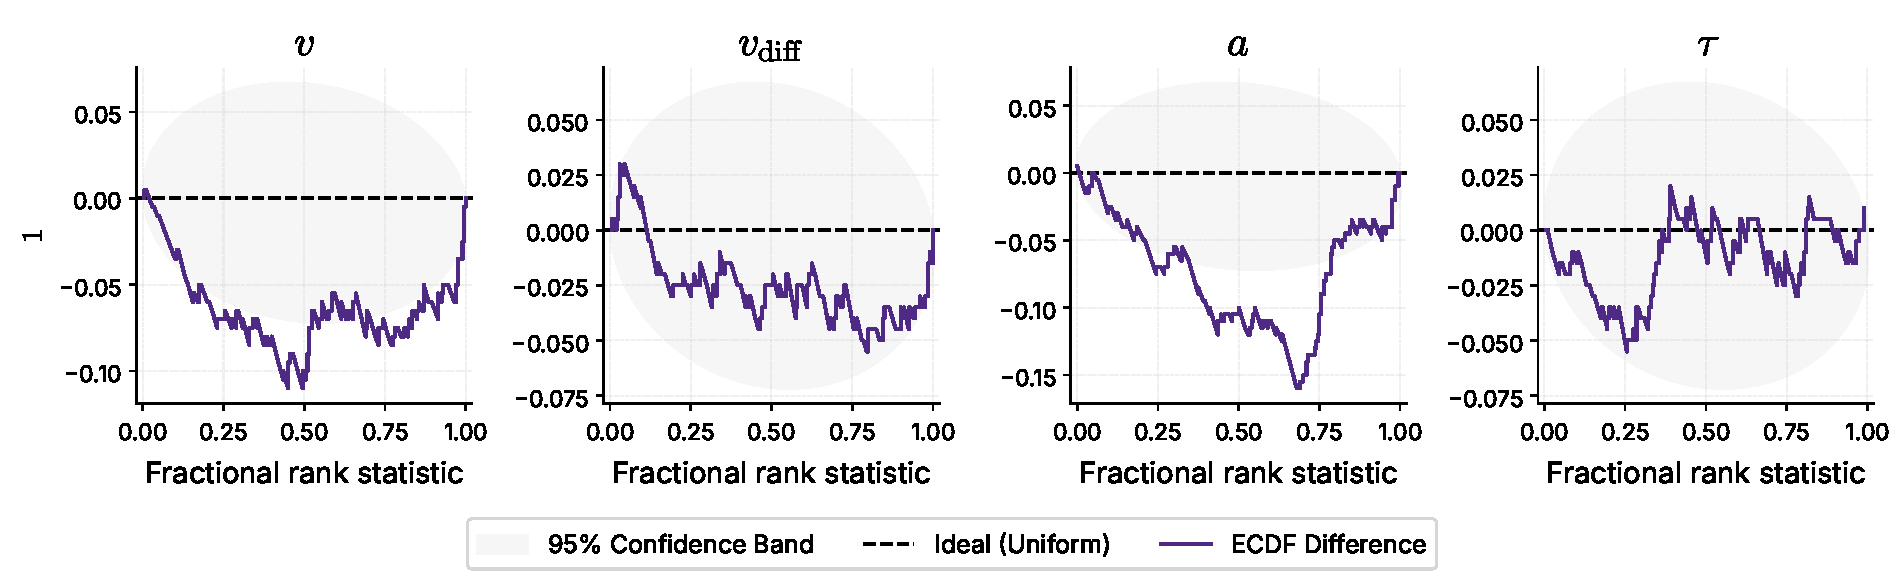
\includegraphics[width=\textwidth,height=0.3\textheight,keepaspectratio]{rdm/fixed/cf_ecdf.pdf}\par\vspace{1ex}
  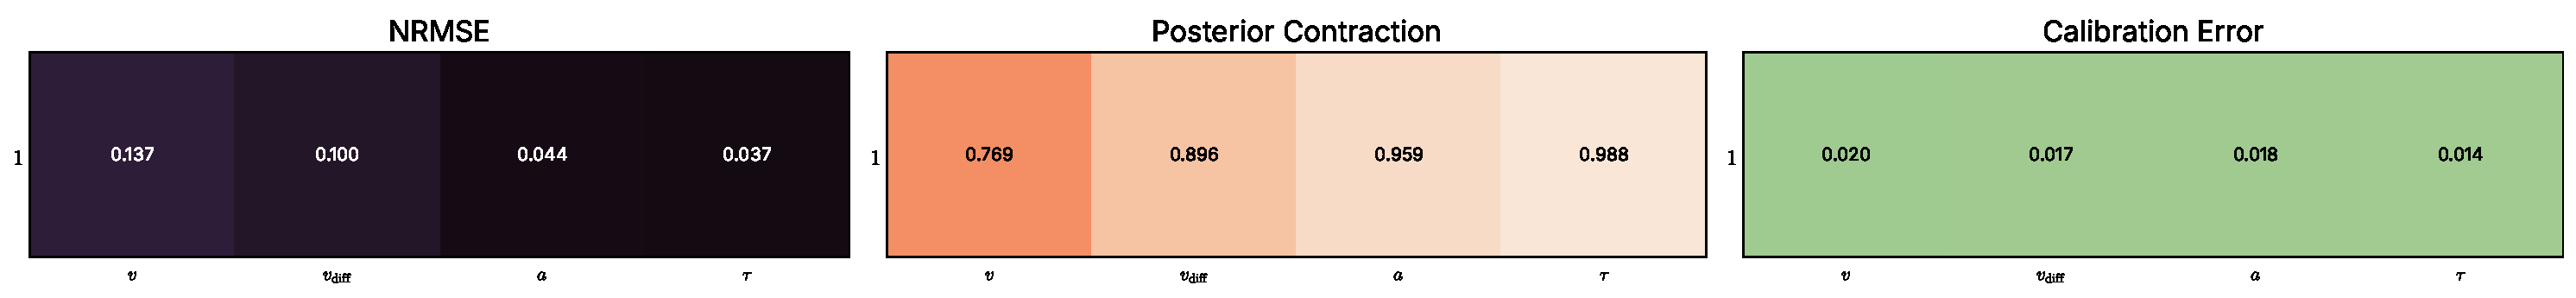
\includegraphics[width=\textwidth]{rdm/fixed/cf_metrics.pdf}
  \caption{\textbf{RDM, \emph{fixed} design: CogFormer.} Recovery (top), calibration (middle), metrics (bottom). $s_v$ and $s_\tau$ are fixed at 0 and not estimated; every estimated parameter enters as an intercept only (4 coefficients shown). Layout and encoding as in Figure~\ref{fig:app1-ddm-intercept-only-cf}.}
  \label{fig:app1-rdm-fixed-cf}
\end{figure}

\begin{figure}[p]
  \centering
  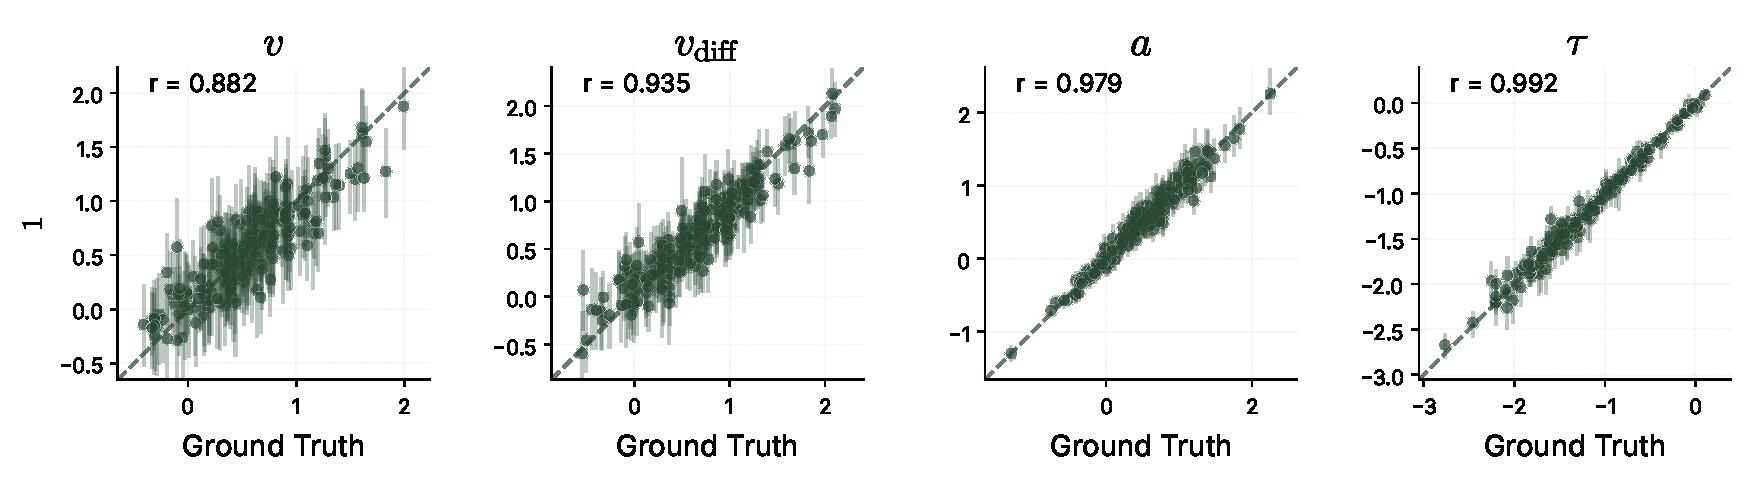
\includegraphics[width=\textwidth,height=0.3\textheight,keepaspectratio]{rdm/fixed/bf_recovery.pdf}\par\vspace{1ex}
  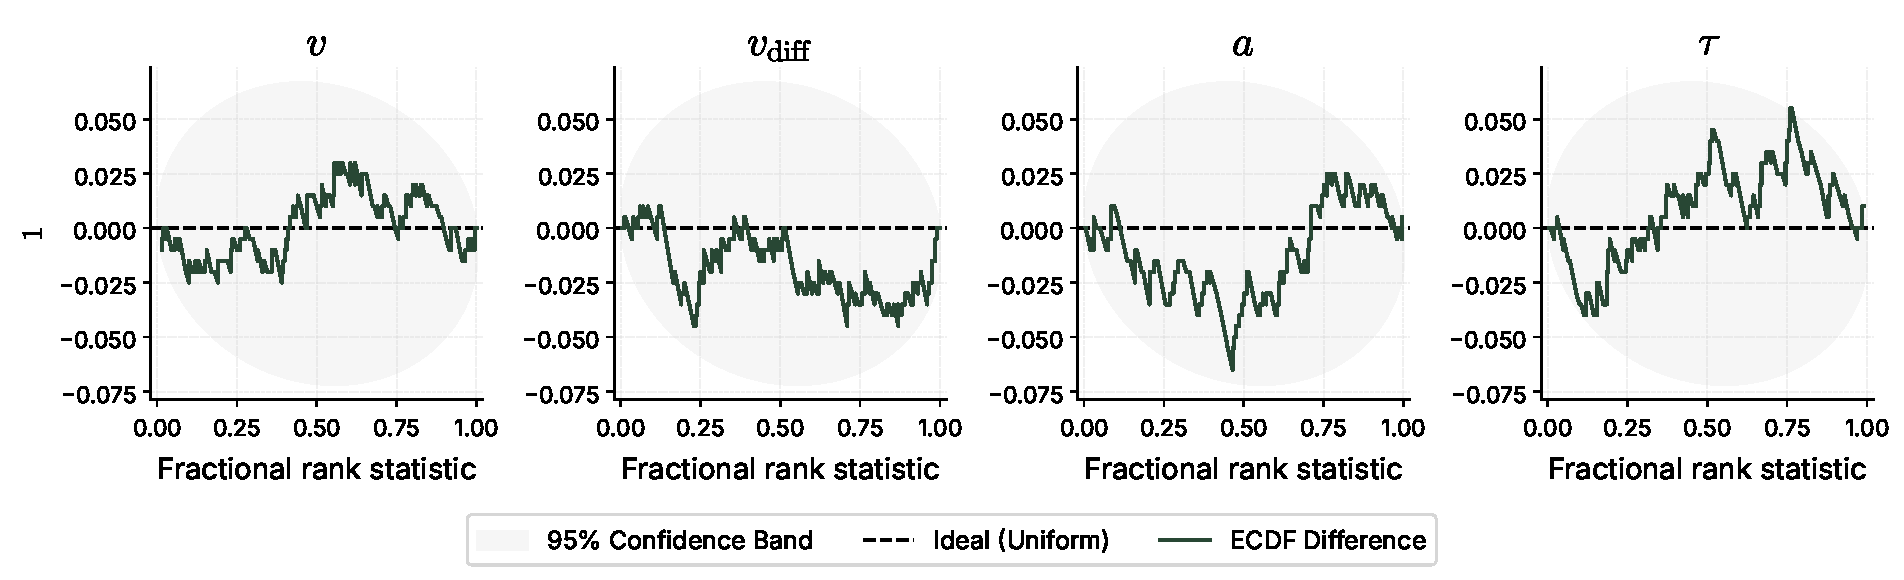
\includegraphics[width=\textwidth,height=0.3\textheight,keepaspectratio]{rdm/fixed/bf_ecdf.pdf}\par\vspace{1ex}
  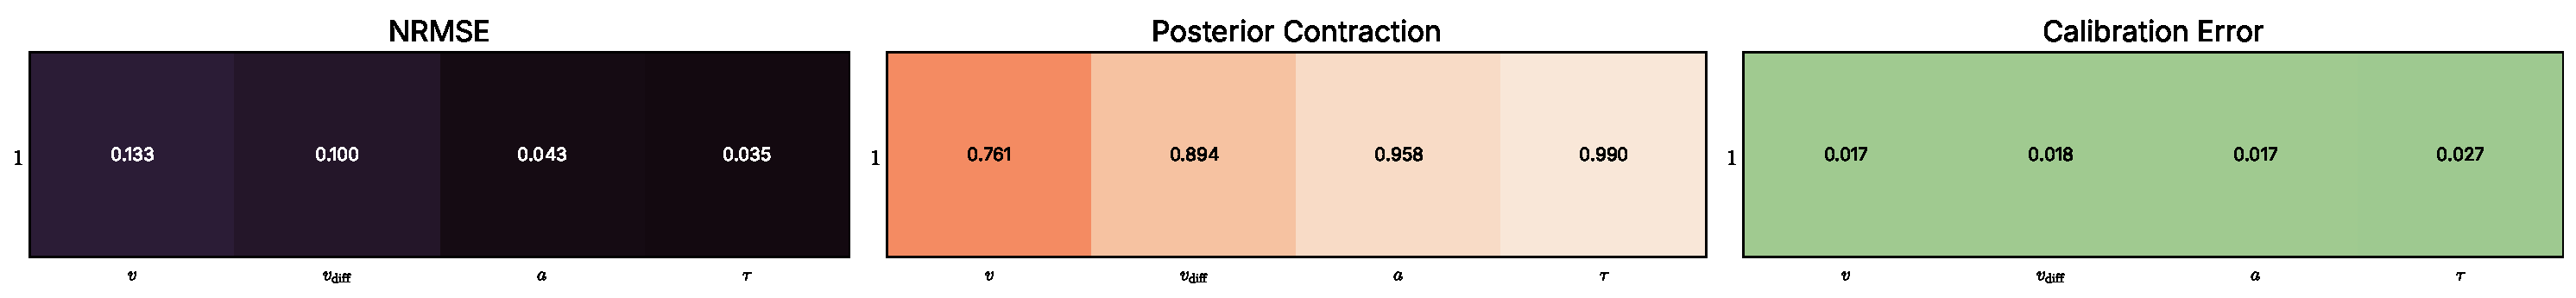
\includegraphics[width=\textwidth]{rdm/fixed/bf_metrics.pdf}
  \caption{\textbf{RDM, \emph{fixed} design: BayesFlow baseline.} Recovery (top), calibration (middle), metrics (bottom). $s_v$ and $s_\tau$ are fixed at 0 and not estimated; every estimated parameter enters as an intercept only (4 coefficients shown). Layout and encoding as in Figure~\ref{fig:app1-ddm-intercept-only-cf}.}
  \label{fig:app1-rdm-fixed-bf}
\end{figure}

\begin{figure}[p]
  \centering
  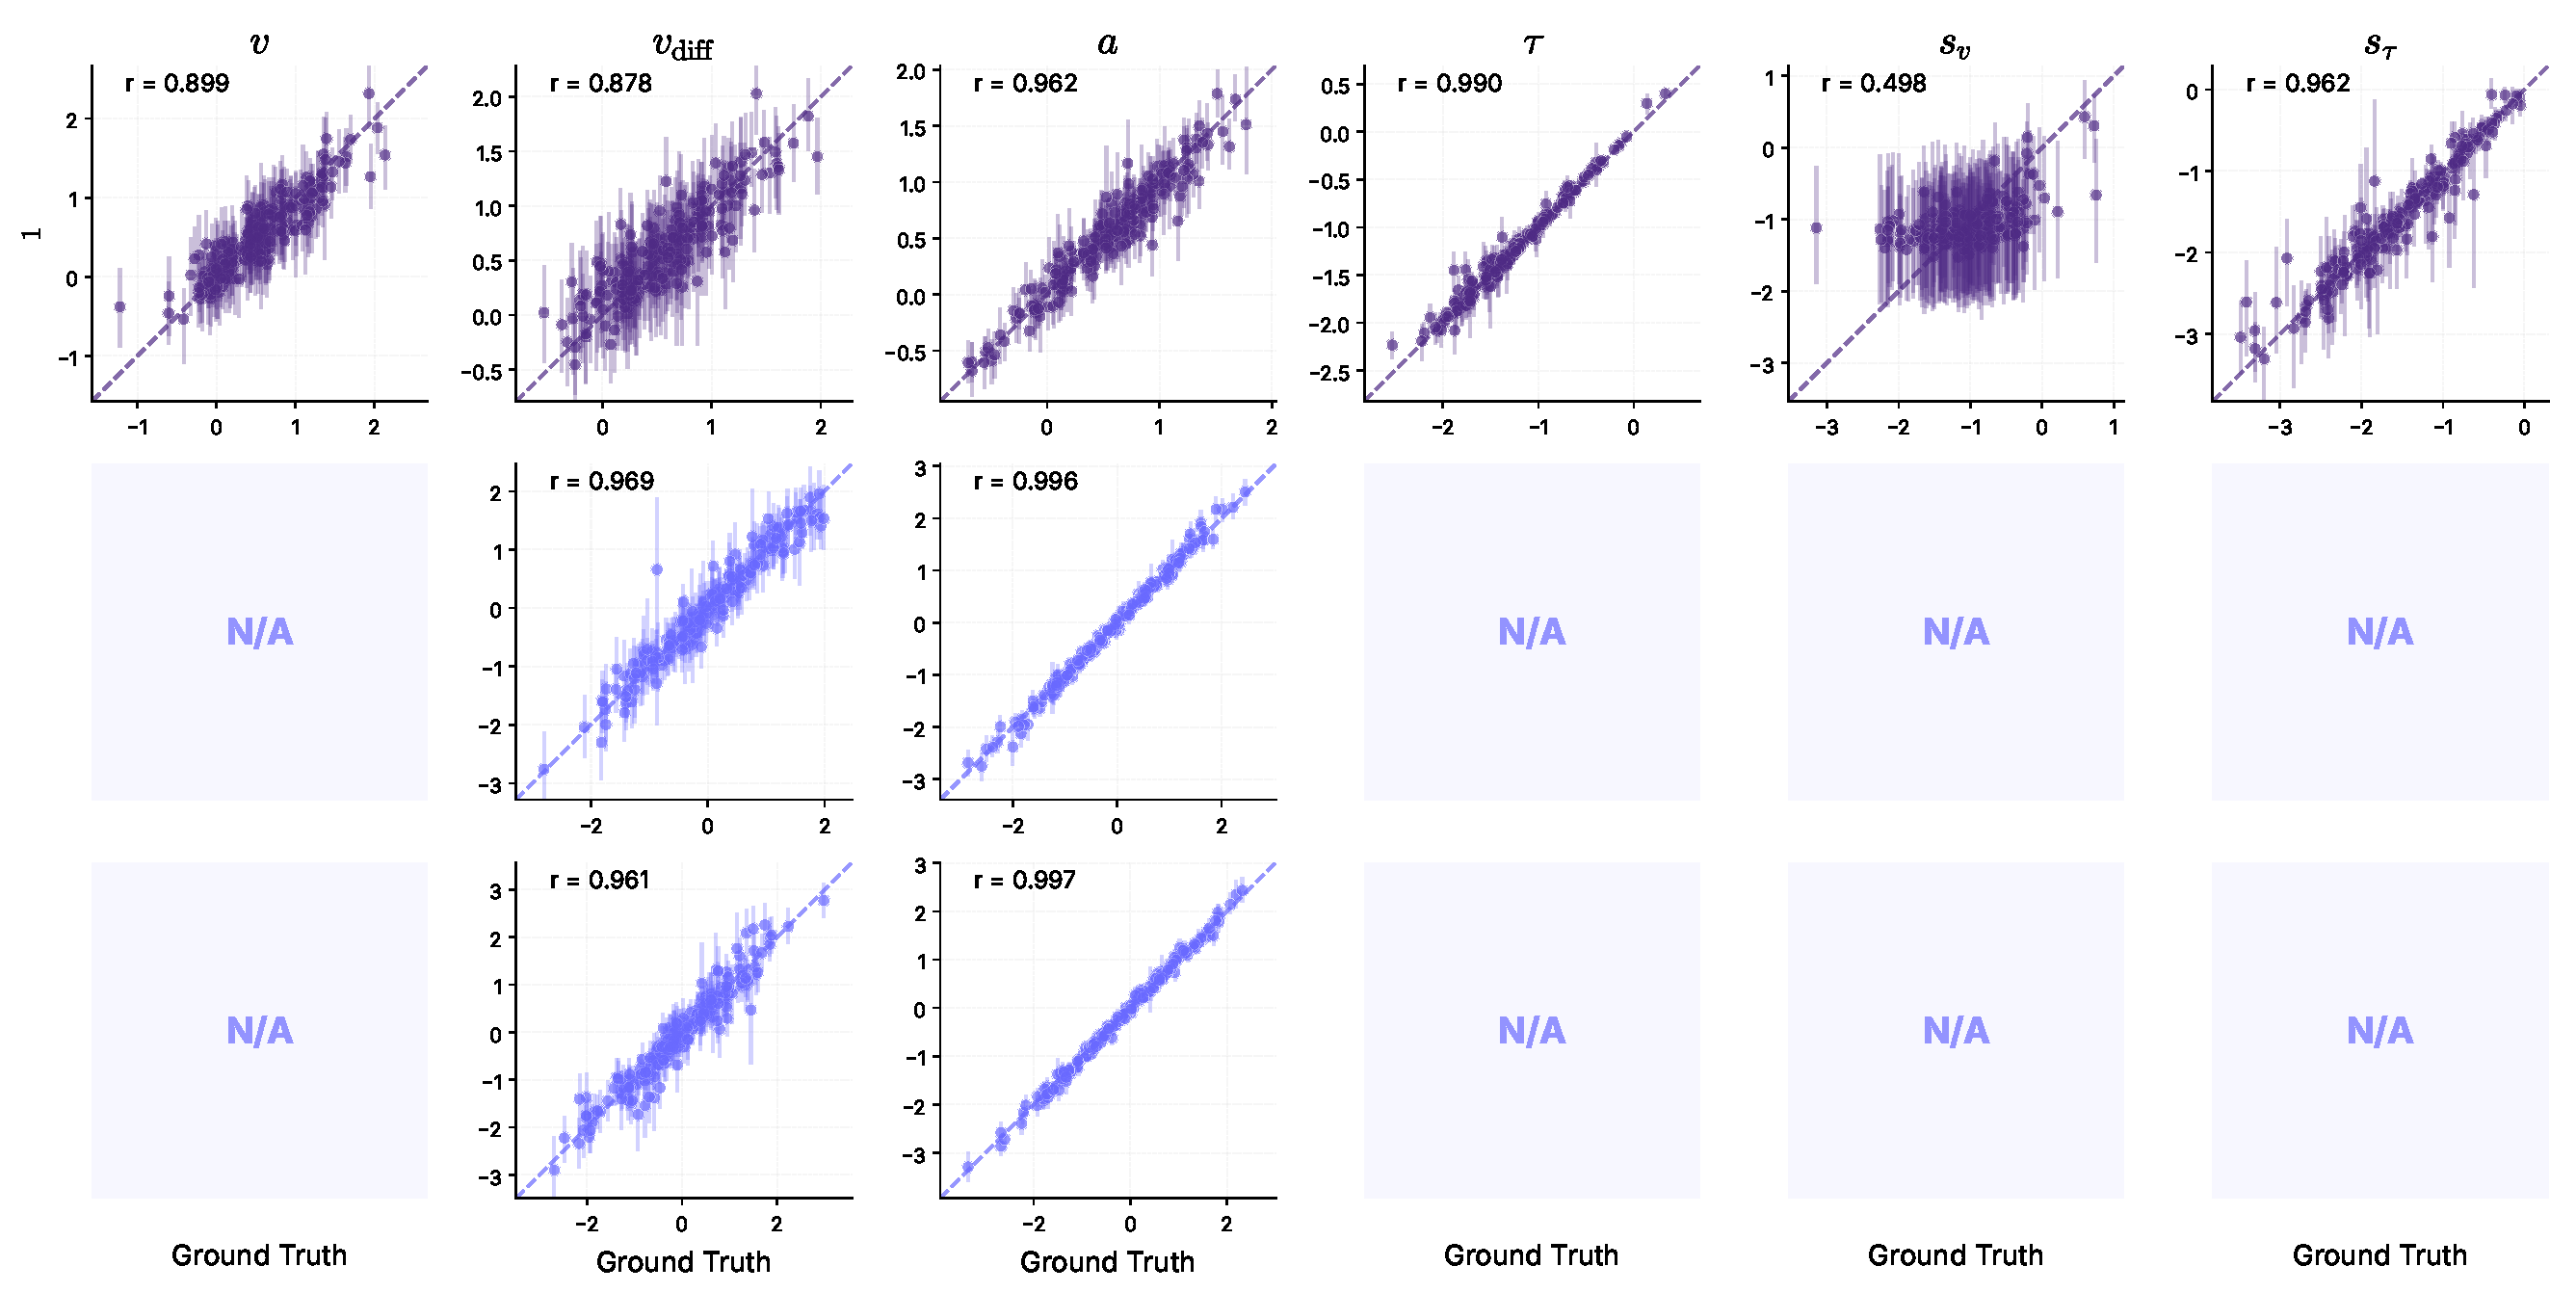
\includegraphics[width=\textwidth,height=0.3\textheight,keepaspectratio]{rdm/regressed/cf_recovery.pdf}\par\vspace{1ex}
  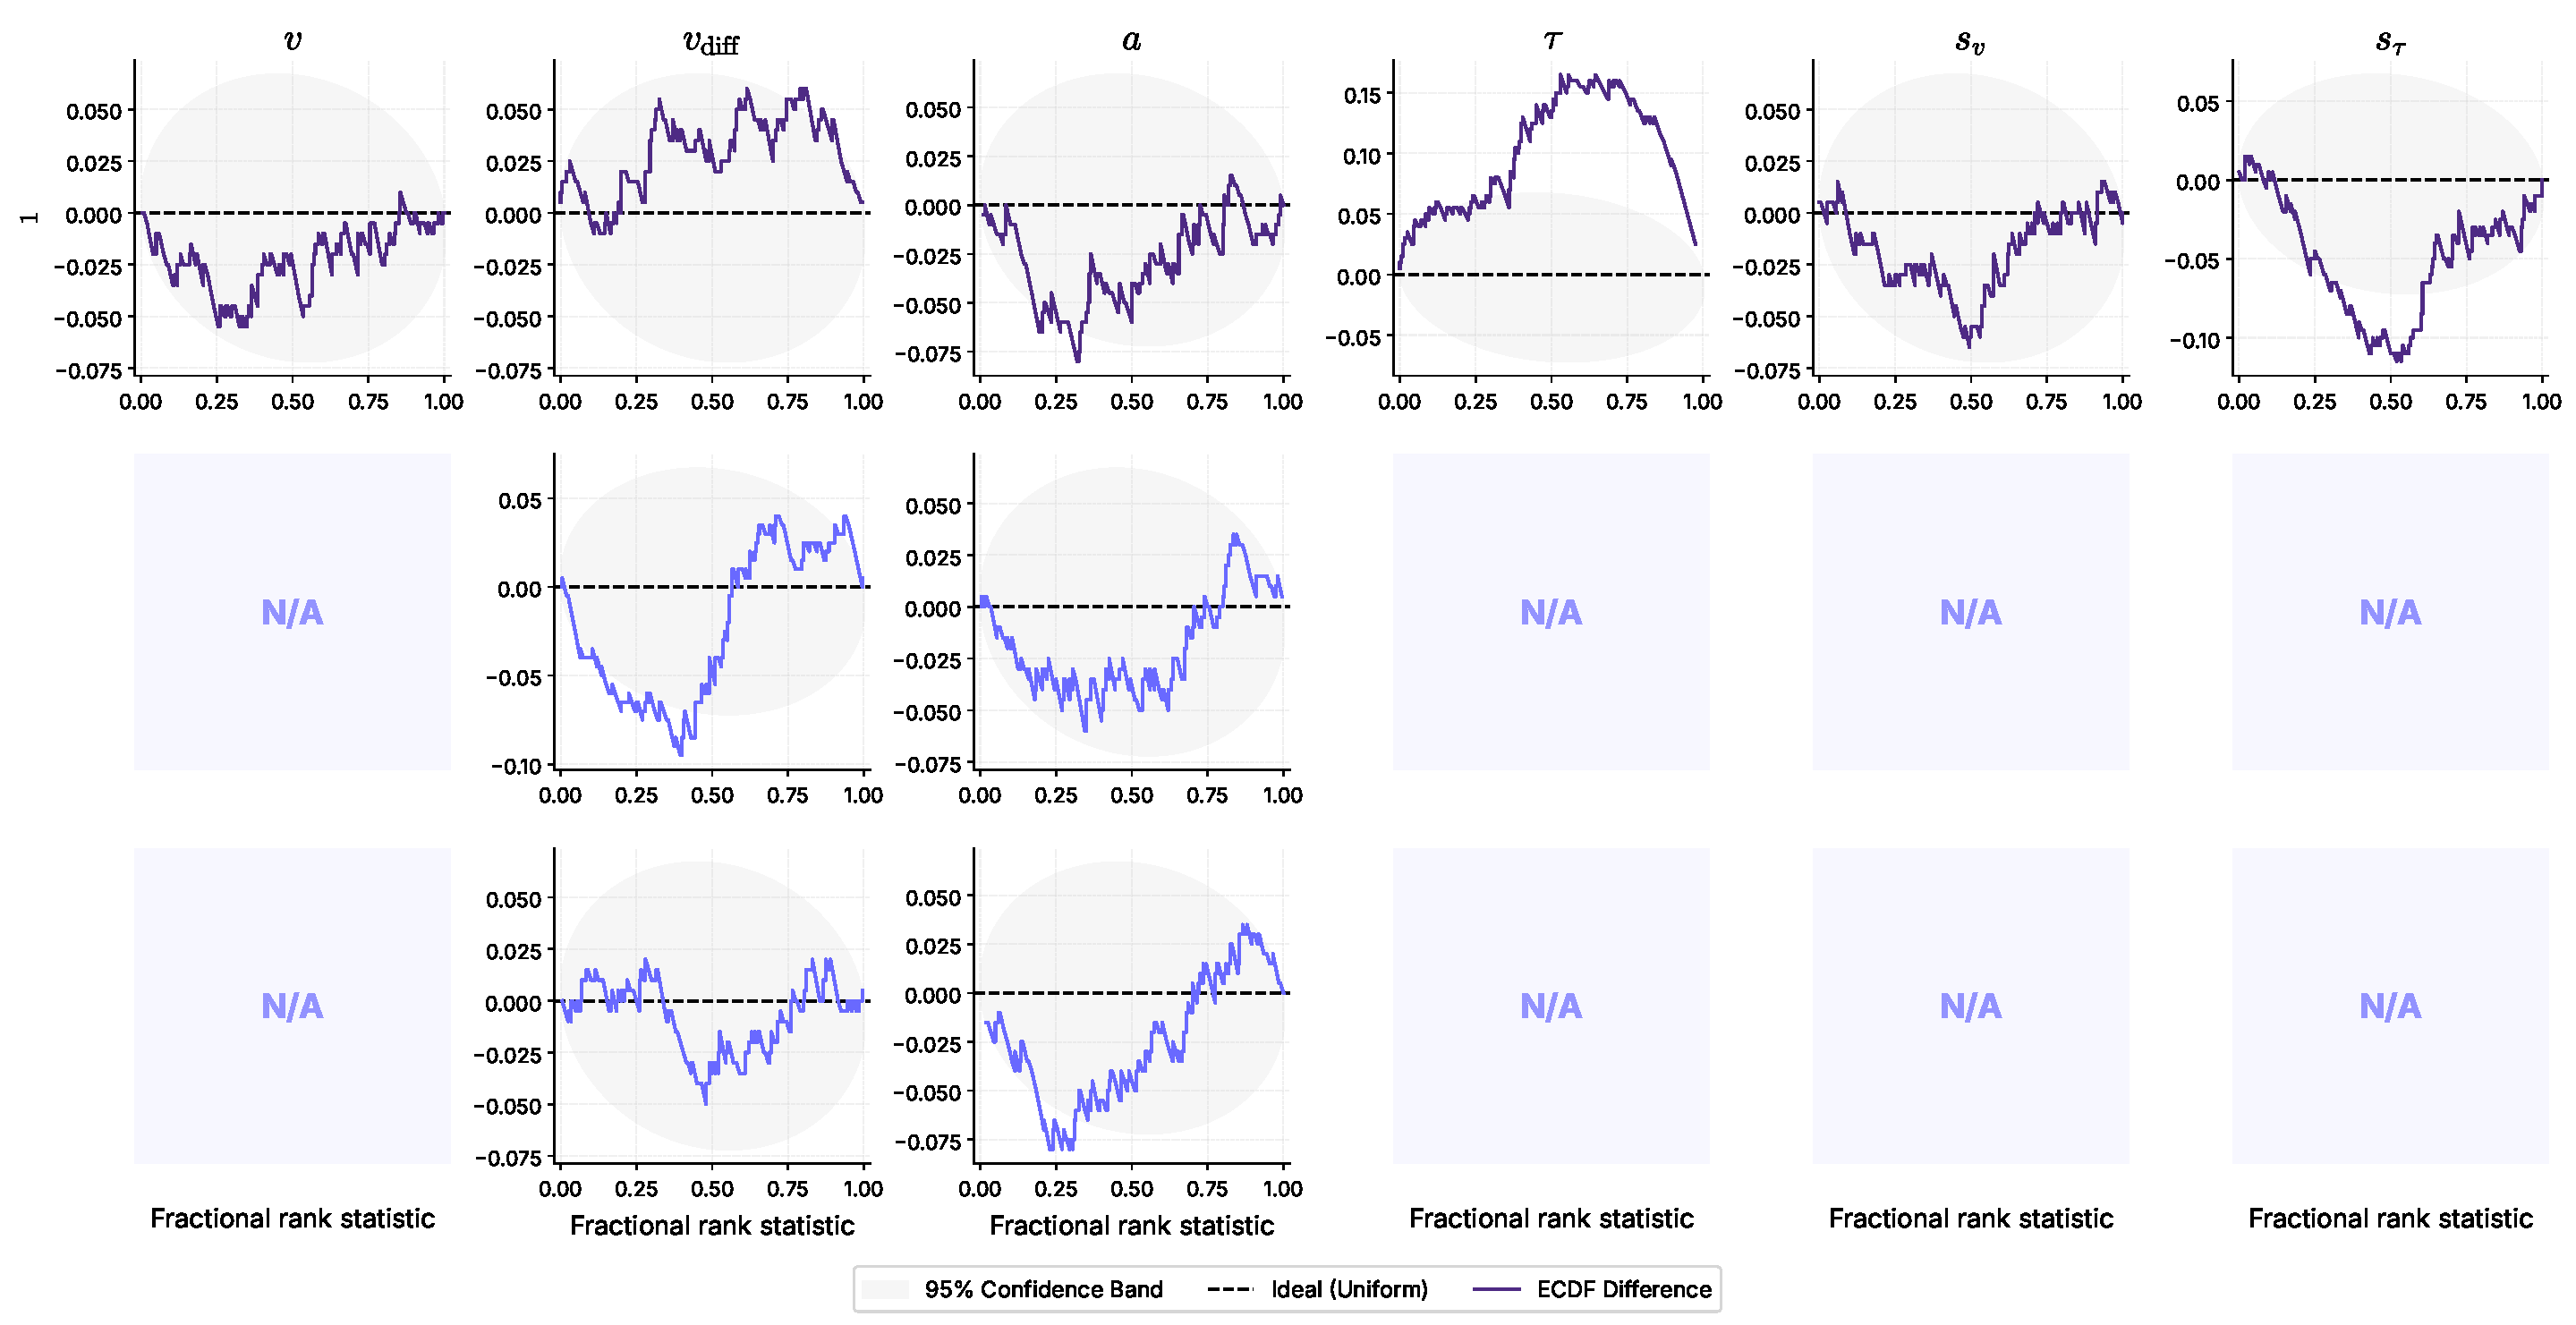
\includegraphics[width=\textwidth,height=0.3\textheight,keepaspectratio]{rdm/regressed/cf_ecdf.pdf}\par\vspace{1ex}
  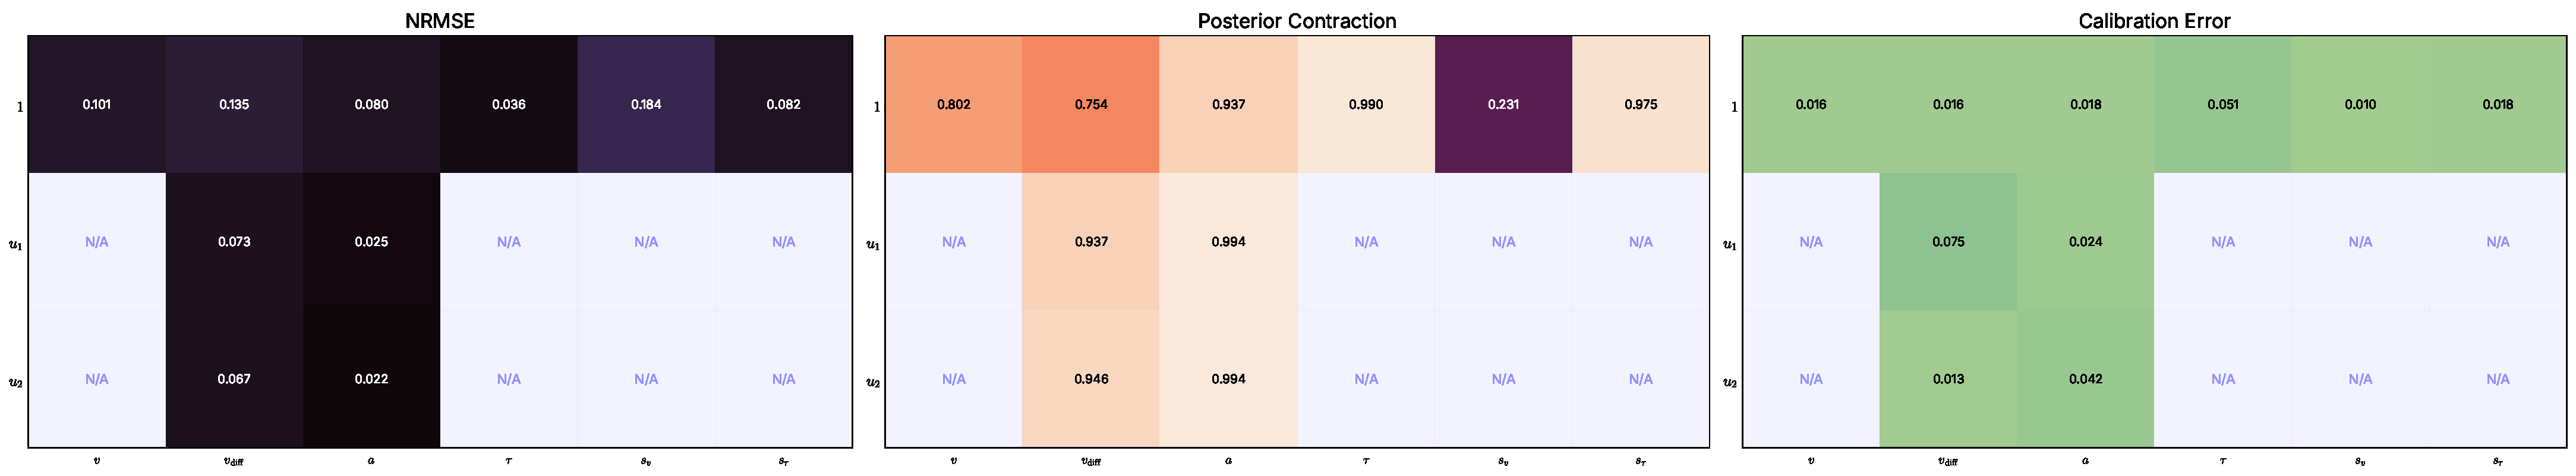
\includegraphics[width=\textwidth]{rdm/regressed/cf_metrics.pdf}
  \caption{\textbf{RDM, \emph{regressed} design: CogFormer.} Recovery (top), calibration (middle), metrics (bottom). $v_{\mathrm{diff}}$ and $a$ carry slopes on $u_1$ and $u_2$ (10 coefficients shown). Layout and encoding as in Figure~\ref{fig:app1-ddm-intercept-only-cf}.}
  \label{fig:app1-rdm-regressed-cf}
\end{figure}

\begin{figure}[p]
  \centering
  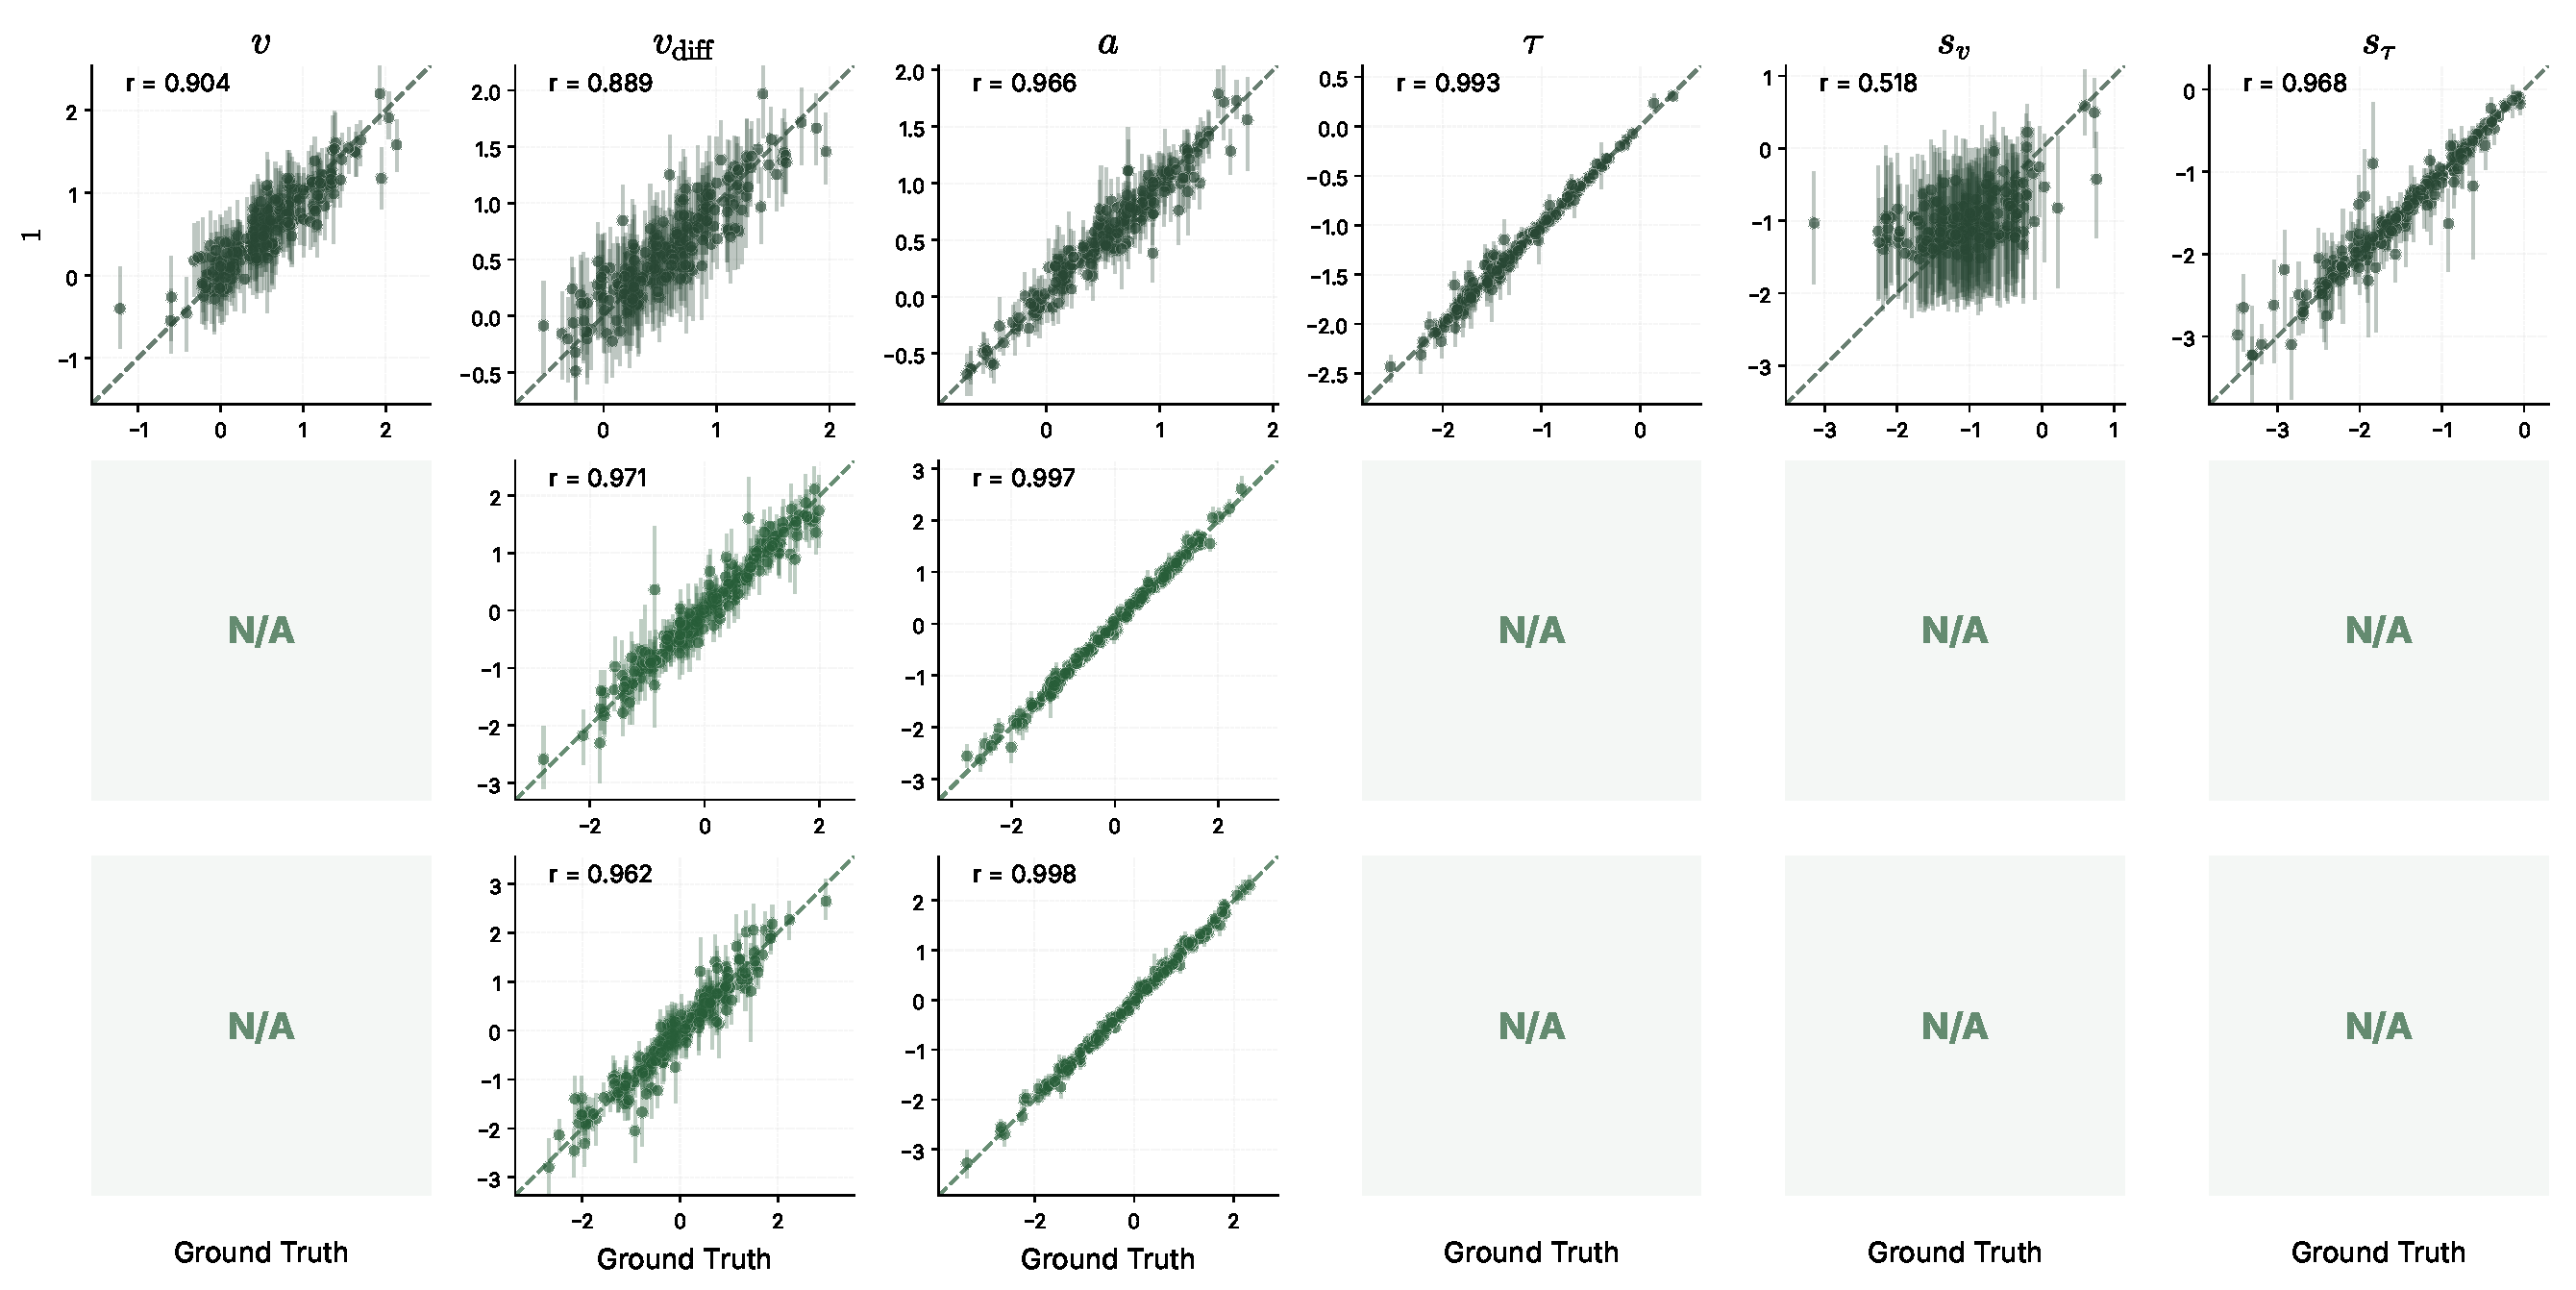
\includegraphics[width=\textwidth,height=0.3\textheight,keepaspectratio]{rdm/regressed/bf_recovery.pdf}\par\vspace{1ex}
  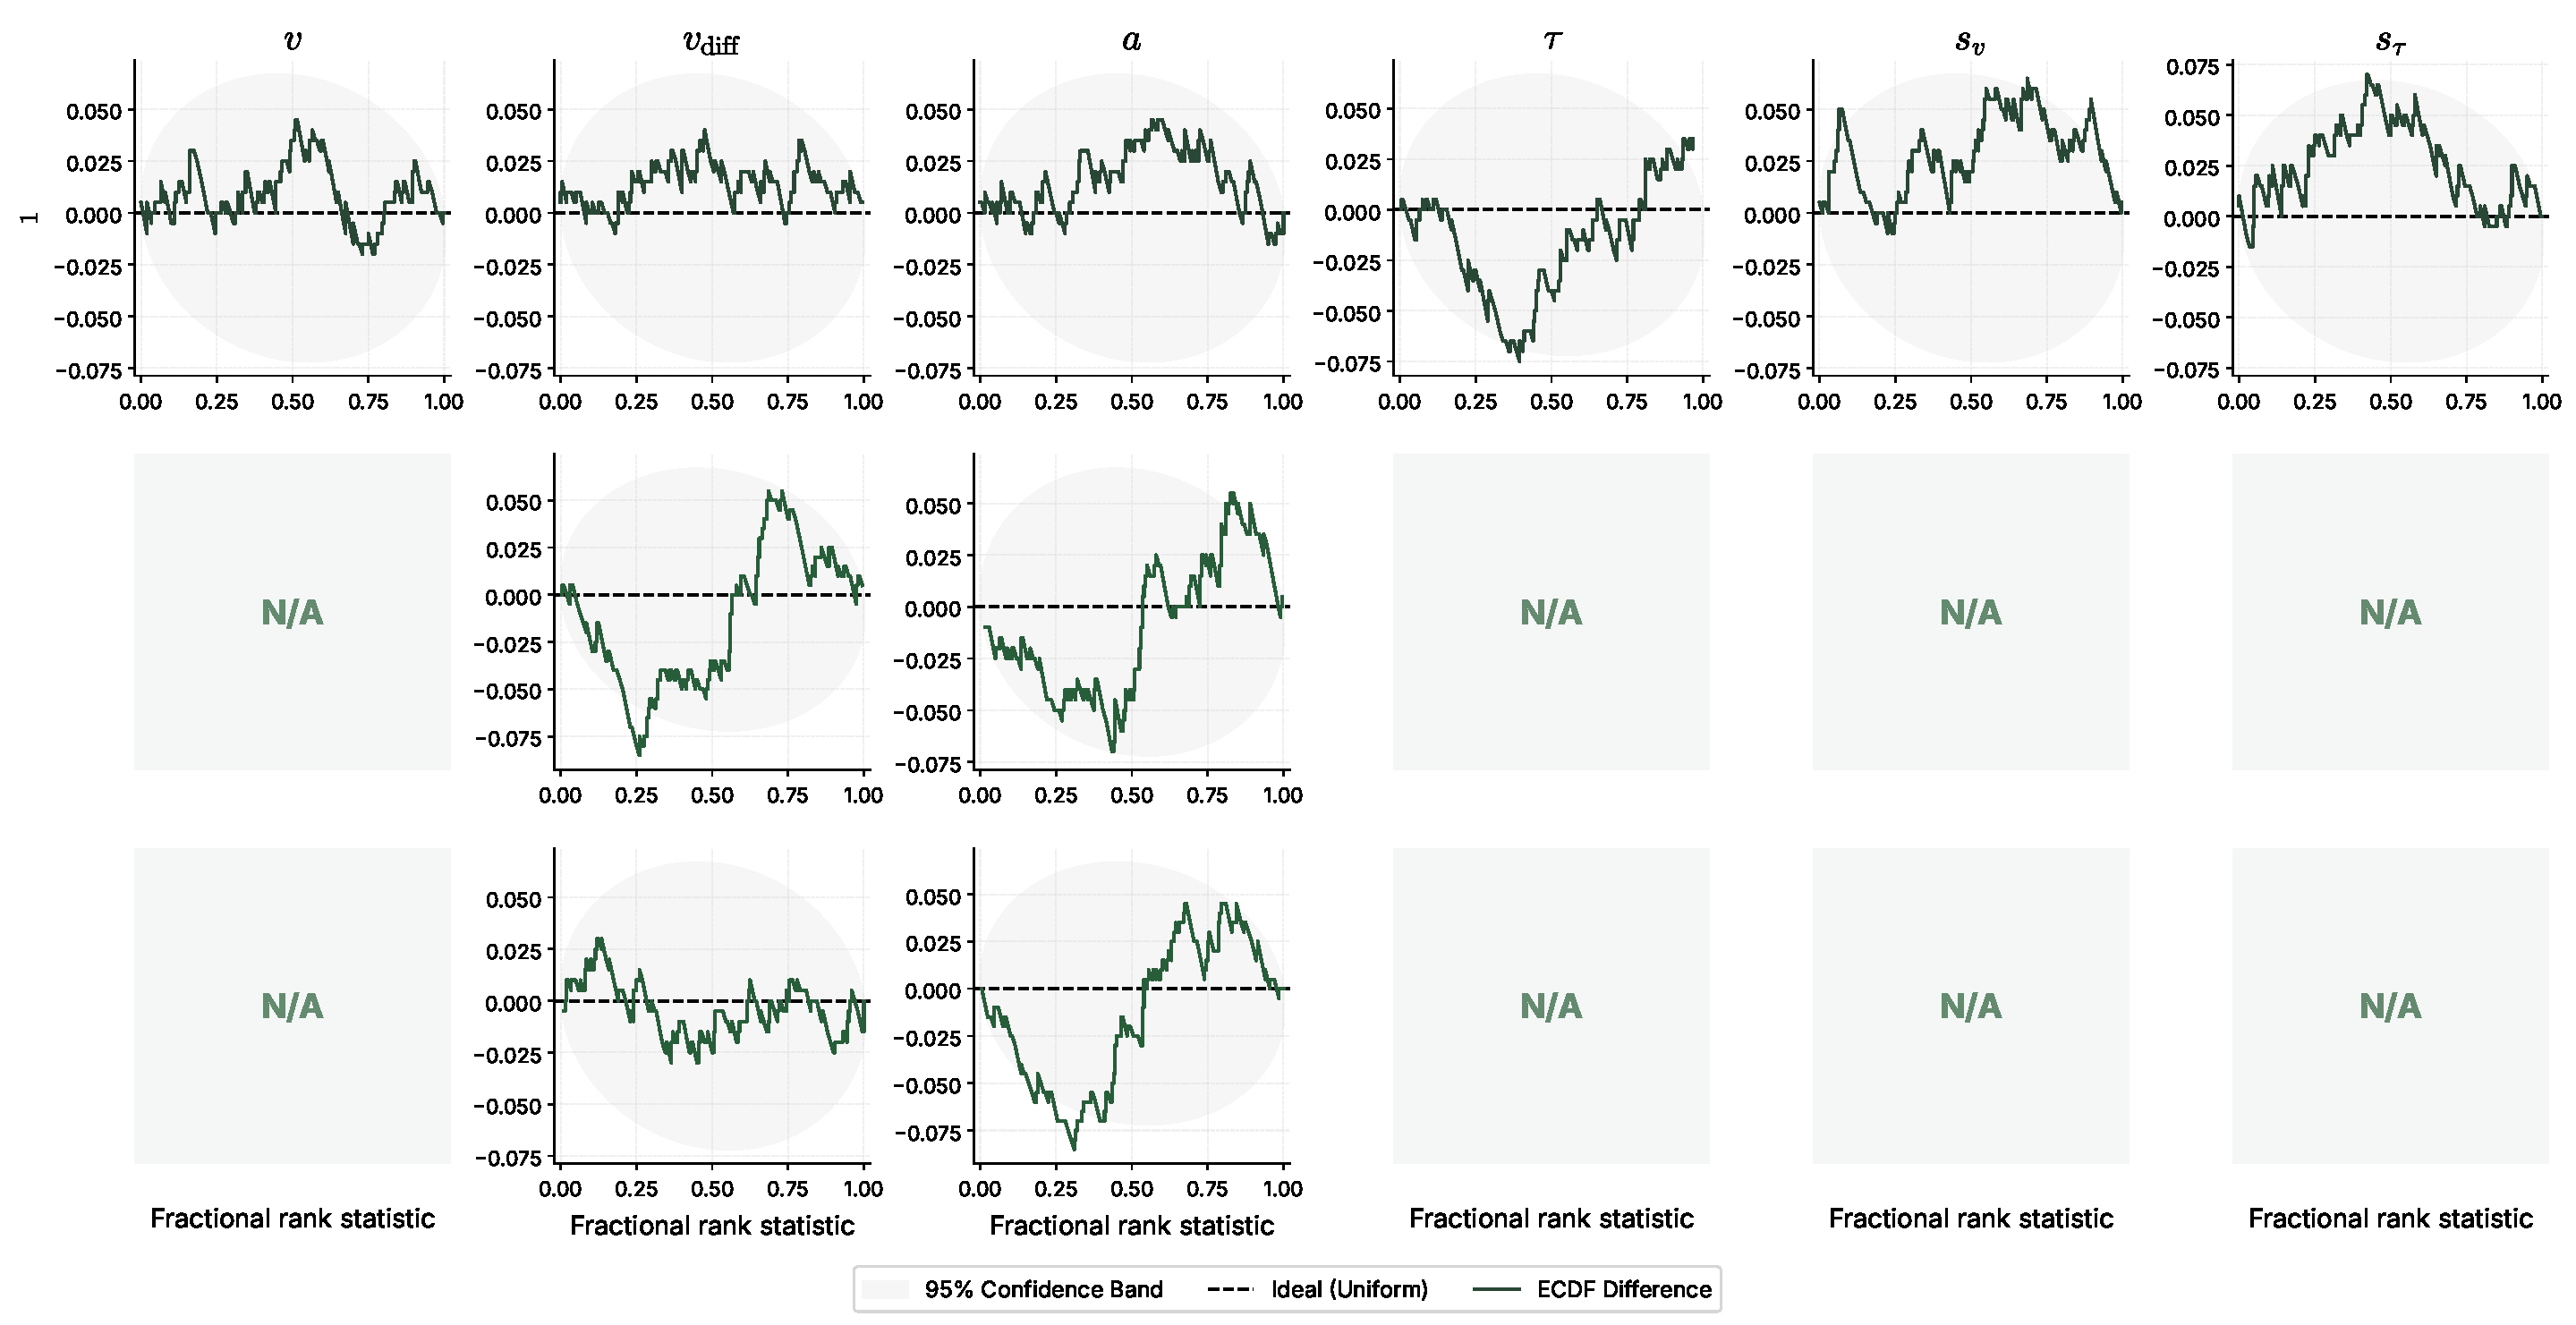
\includegraphics[width=\textwidth,height=0.3\textheight,keepaspectratio]{rdm/regressed/bf_ecdf.pdf}\par\vspace{1ex}
  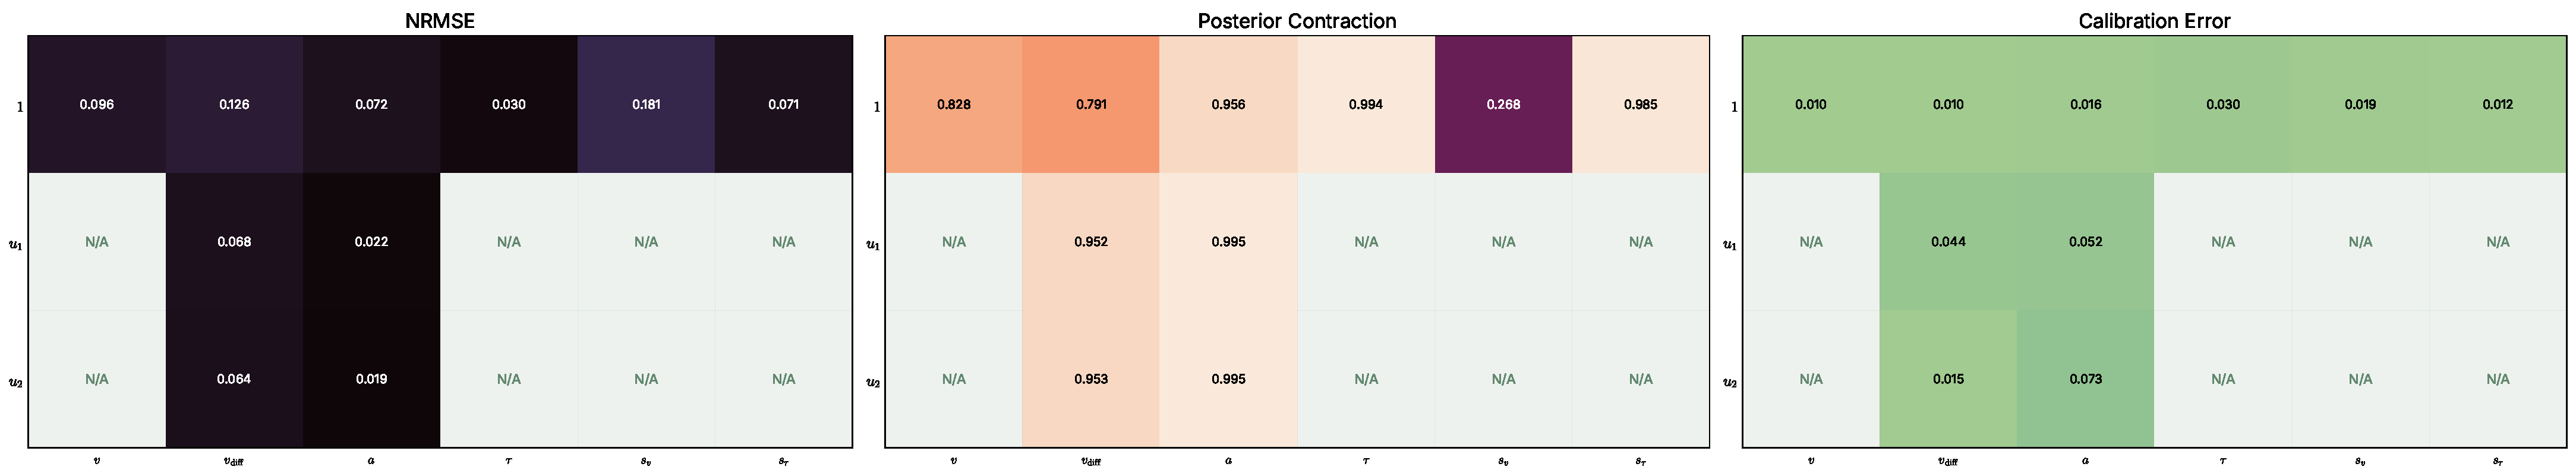
\includegraphics[width=\textwidth]{rdm/regressed/bf_metrics.pdf}
  \caption{\textbf{RDM, \emph{regressed} design: BayesFlow baseline.} Recovery (top), calibration (middle), metrics (bottom). $v_{\mathrm{diff}}$ and $a$ carry slopes on $u_1$ and $u_2$ (10 coefficients shown). Layout and encoding as in Figure~\ref{fig:app1-ddm-intercept-only-cf}.}
  \label{fig:app1-rdm-regressed-bf}
\end{figure}

\begin{figure}[p]
  \centering
  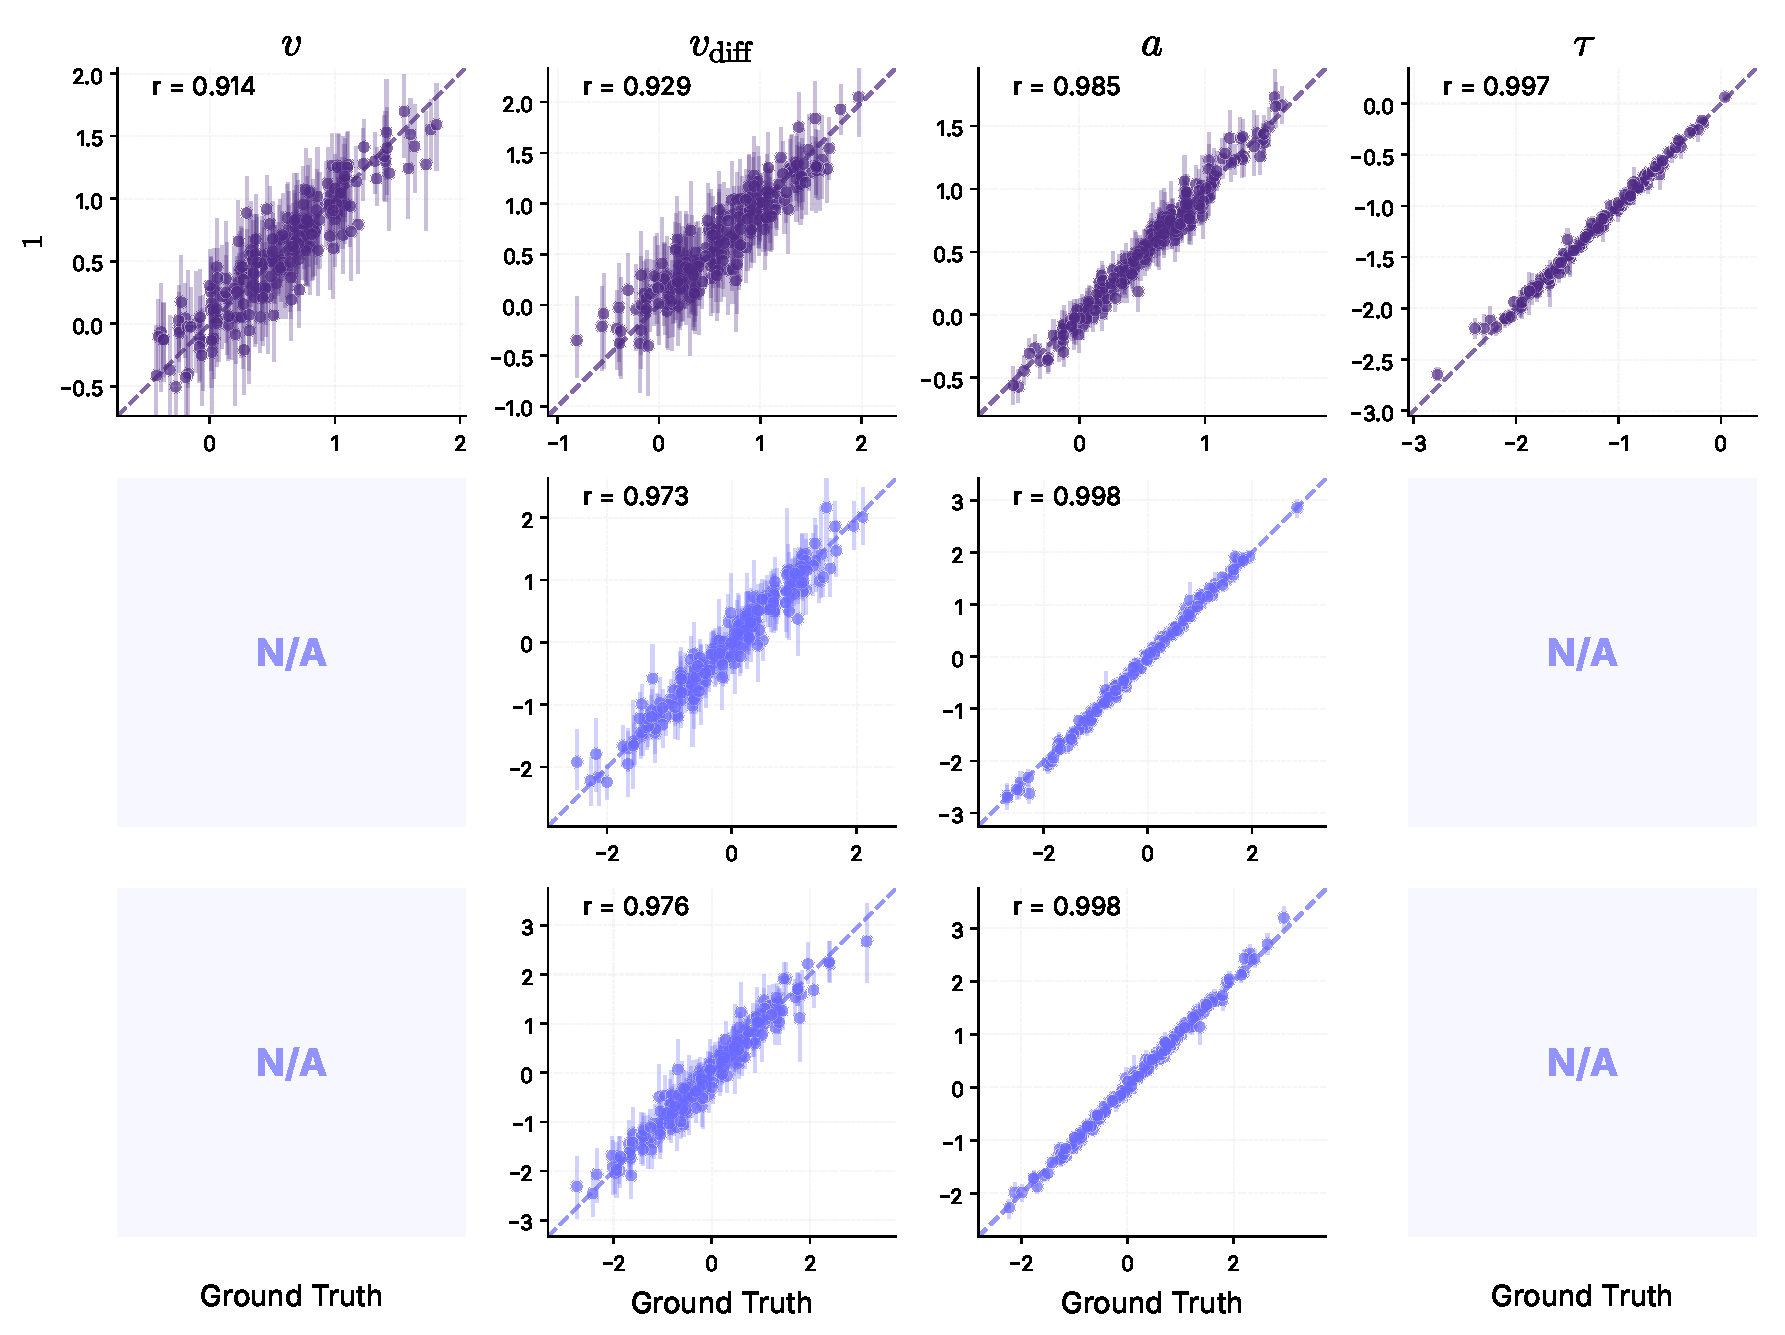
\includegraphics[width=\textwidth,height=0.3\textheight,keepaspectratio]{rdm/fixed_regressed/cf_recovery.pdf}\par\vspace{1ex}
  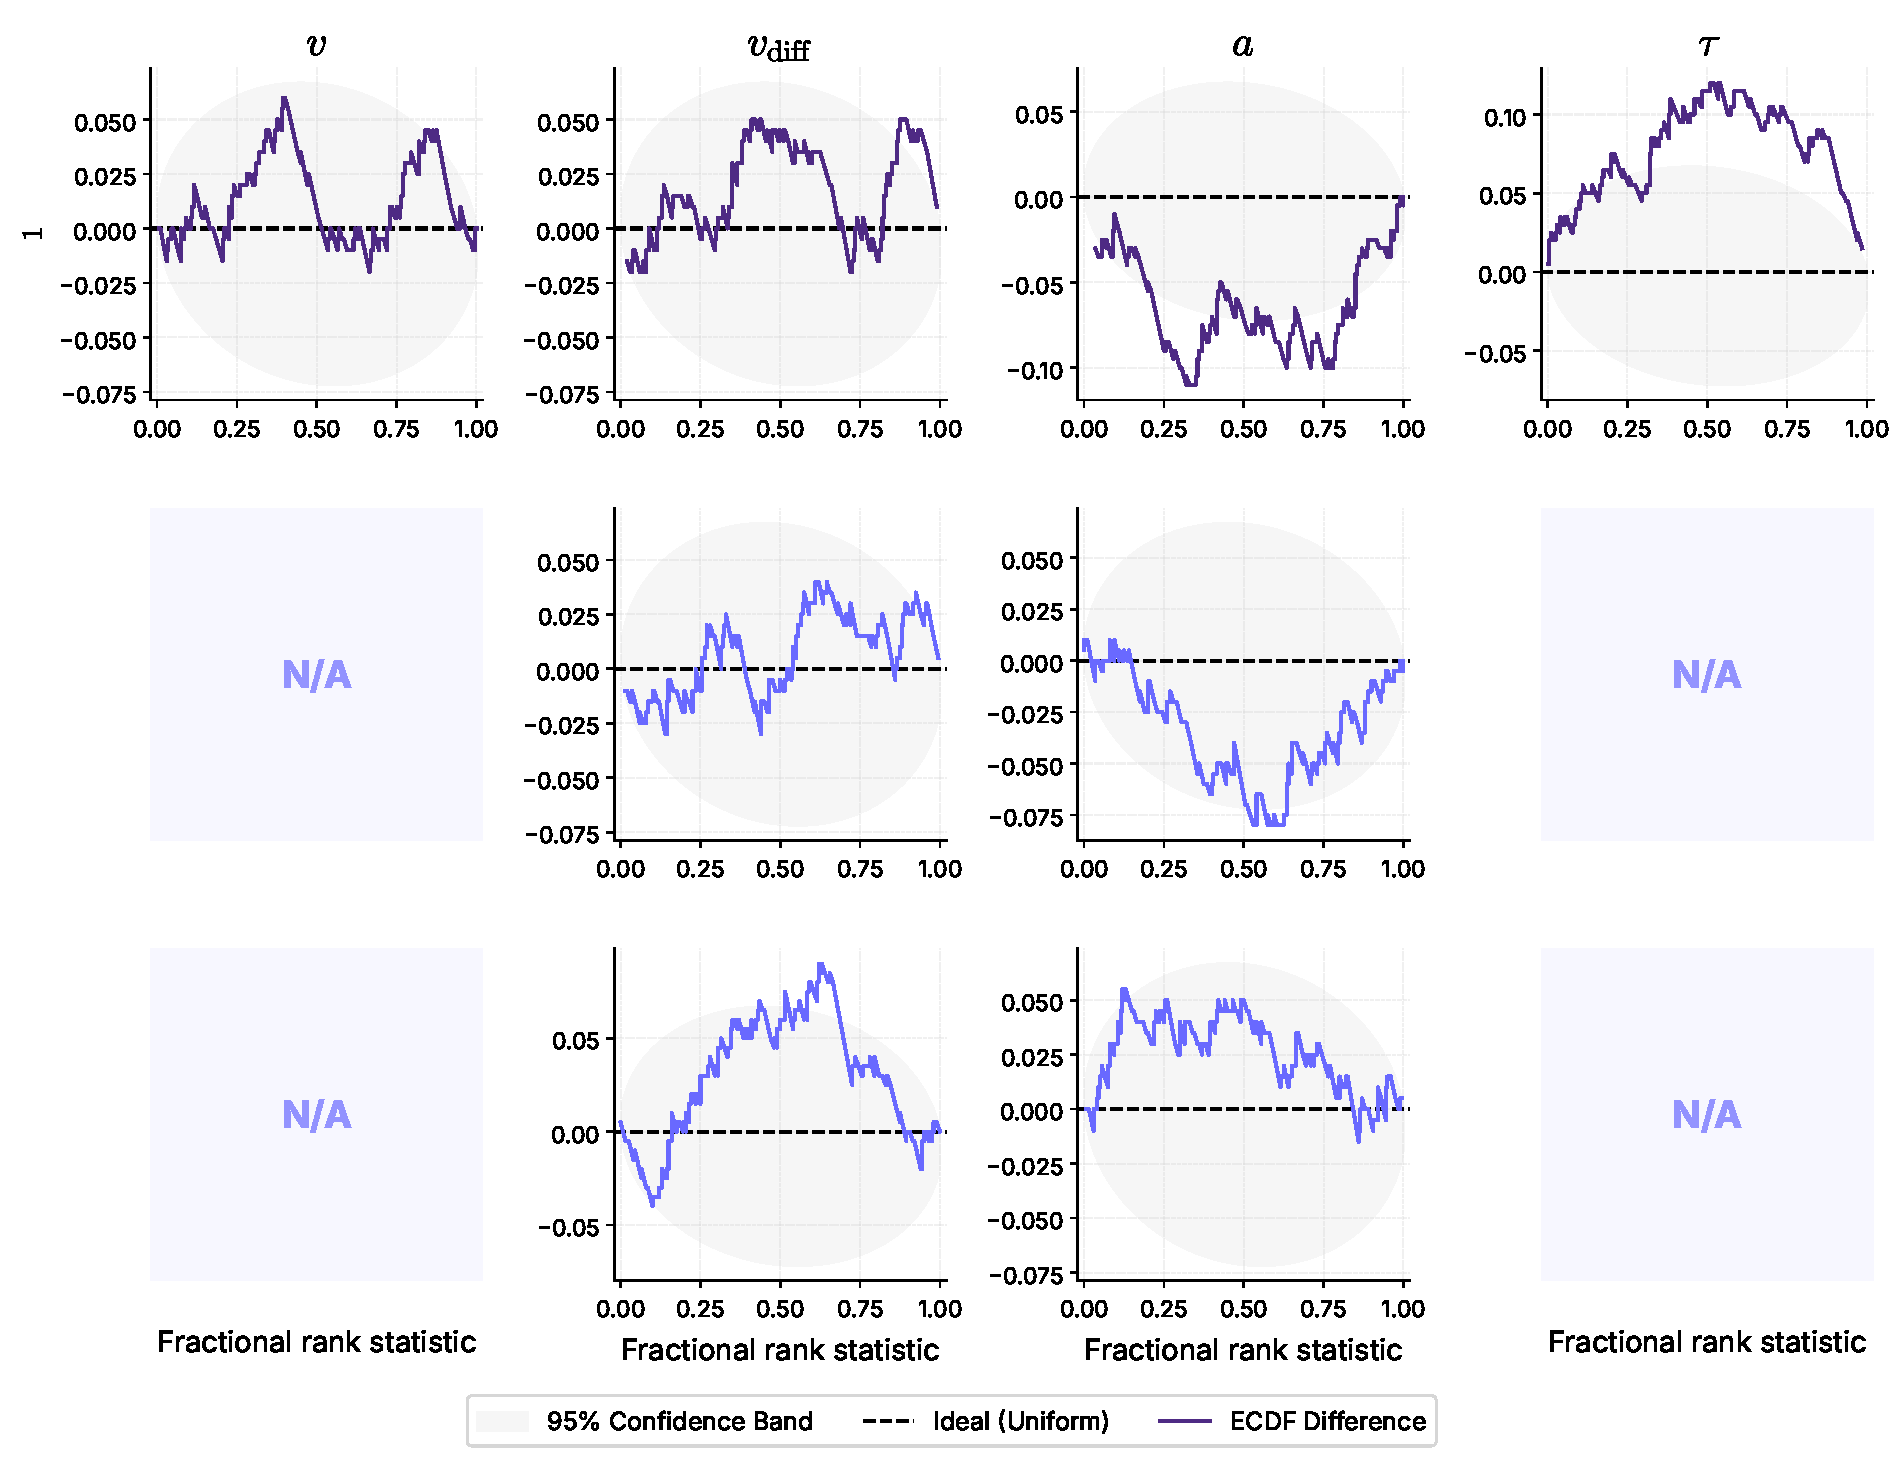
\includegraphics[width=\textwidth,height=0.3\textheight,keepaspectratio]{rdm/fixed_regressed/cf_ecdf.pdf}\par\vspace{1ex}
  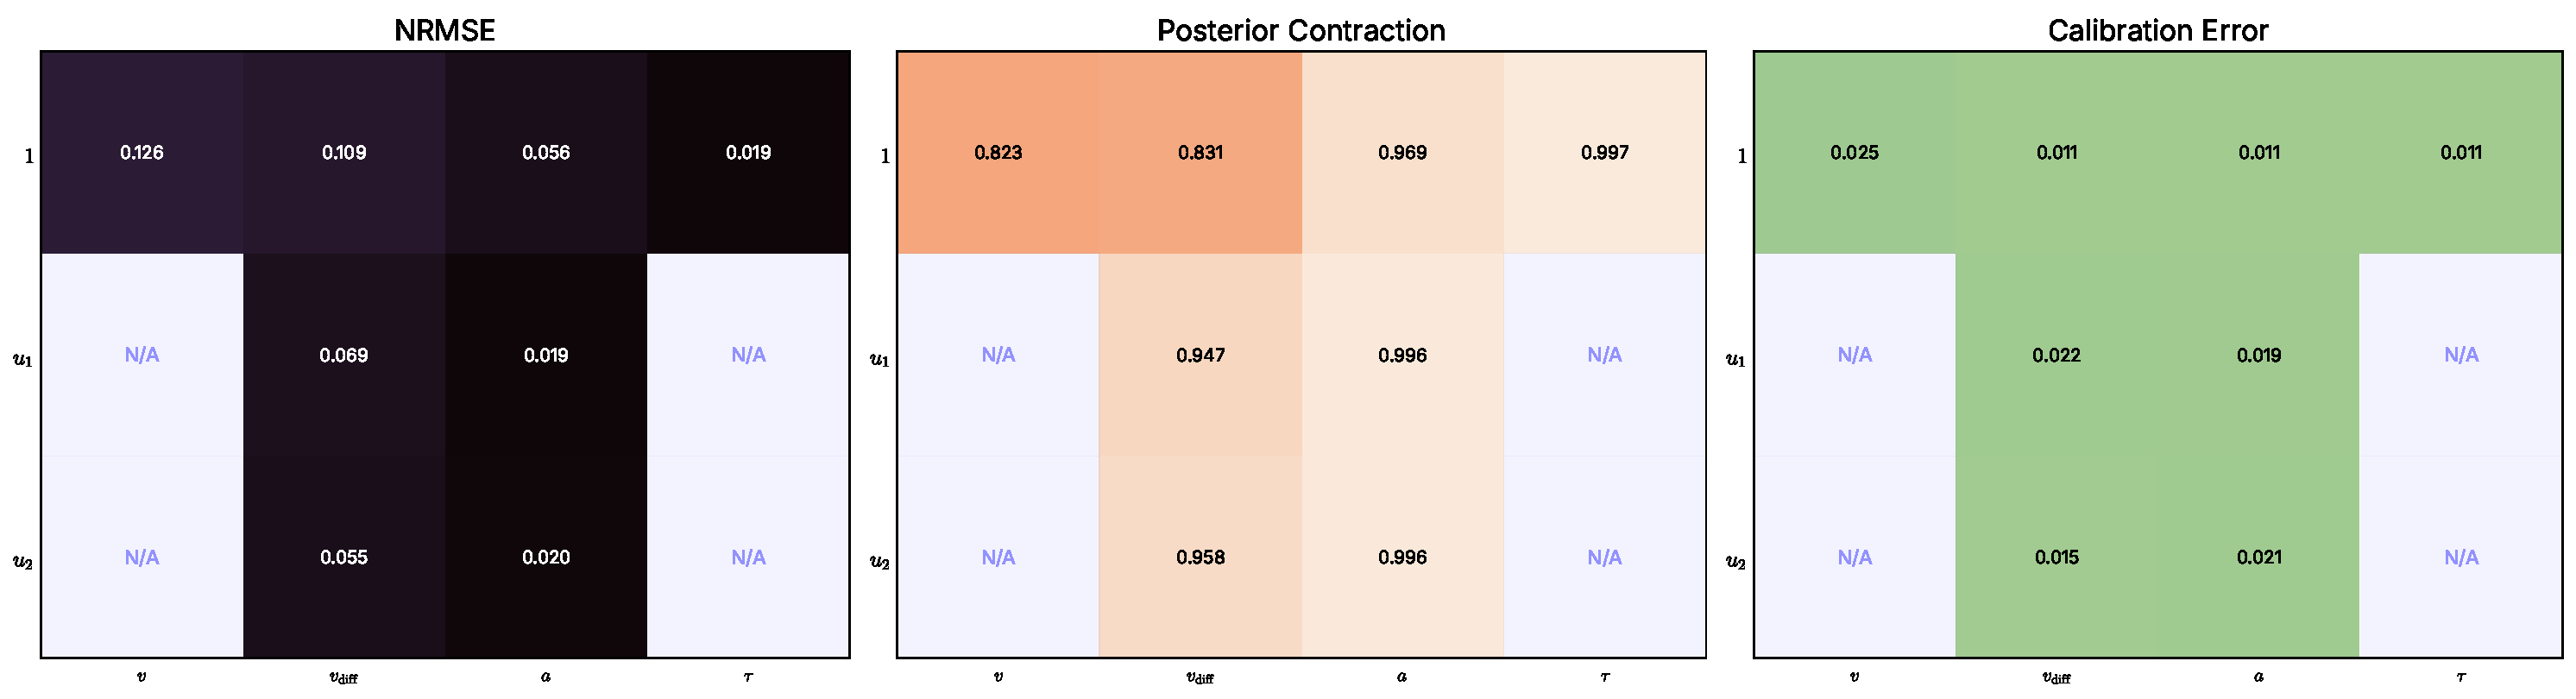
\includegraphics[width=\textwidth]{rdm/fixed_regressed/cf_metrics.pdf}
  \caption{\textbf{RDM, \emph{fixed + regressed} design: CogFormer.} Recovery (top), calibration (middle), metrics (bottom). $s_v$ and $s_\tau$ are fixed at 0 and not estimated; $v_{\mathrm{diff}}$ and $a$ carry slopes on $u_1$ and $u_2$ (8 coefficients shown). Layout and encoding as in Figure~\ref{fig:app1-ddm-intercept-only-cf}.}
  \label{fig:app1-rdm-fixed-regressed-cf}
\end{figure}

\begin{figure}[p]
  \centering
  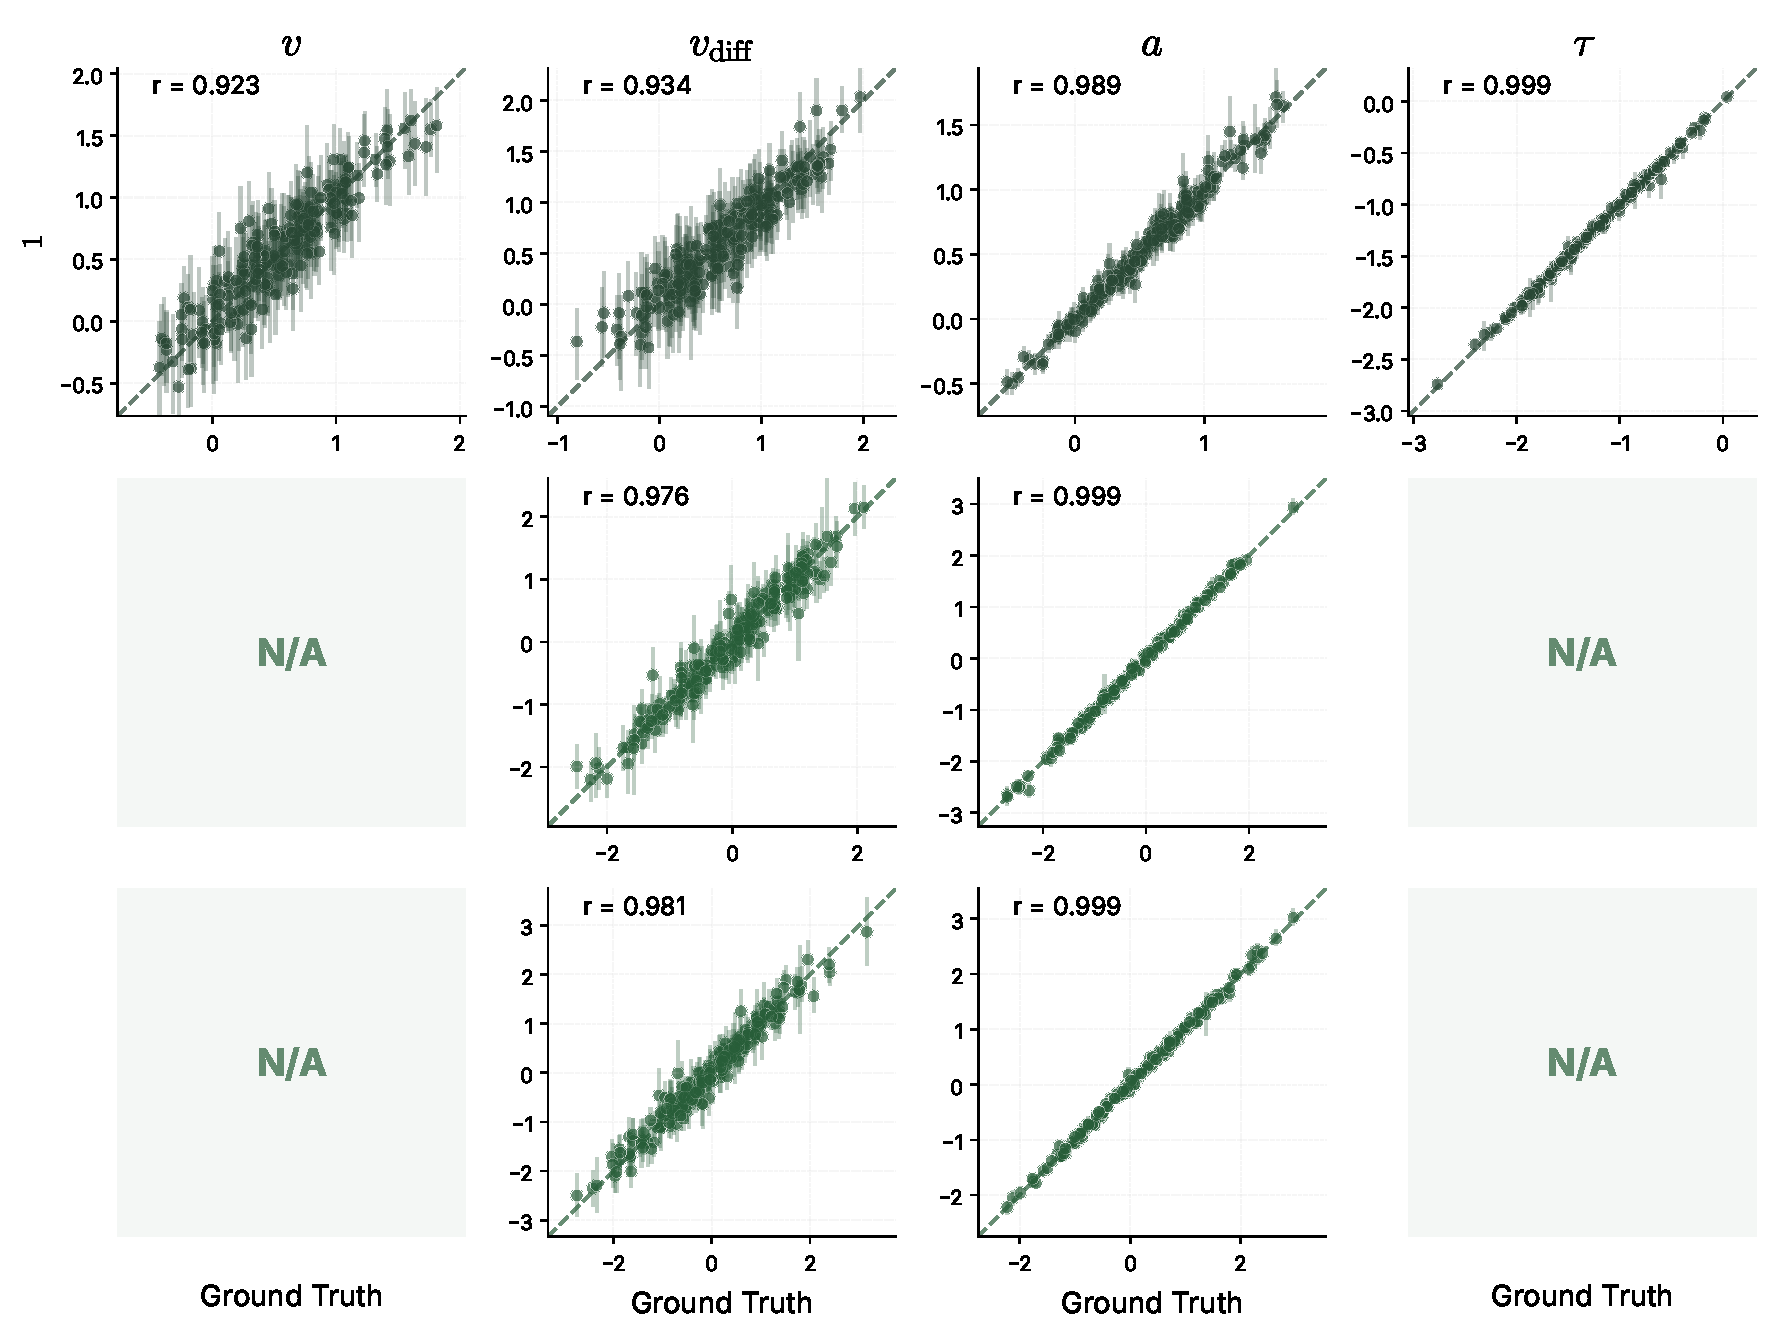
\includegraphics[width=\textwidth,height=0.3\textheight,keepaspectratio]{rdm/fixed_regressed/bf_recovery.pdf}\par\vspace{1ex}
  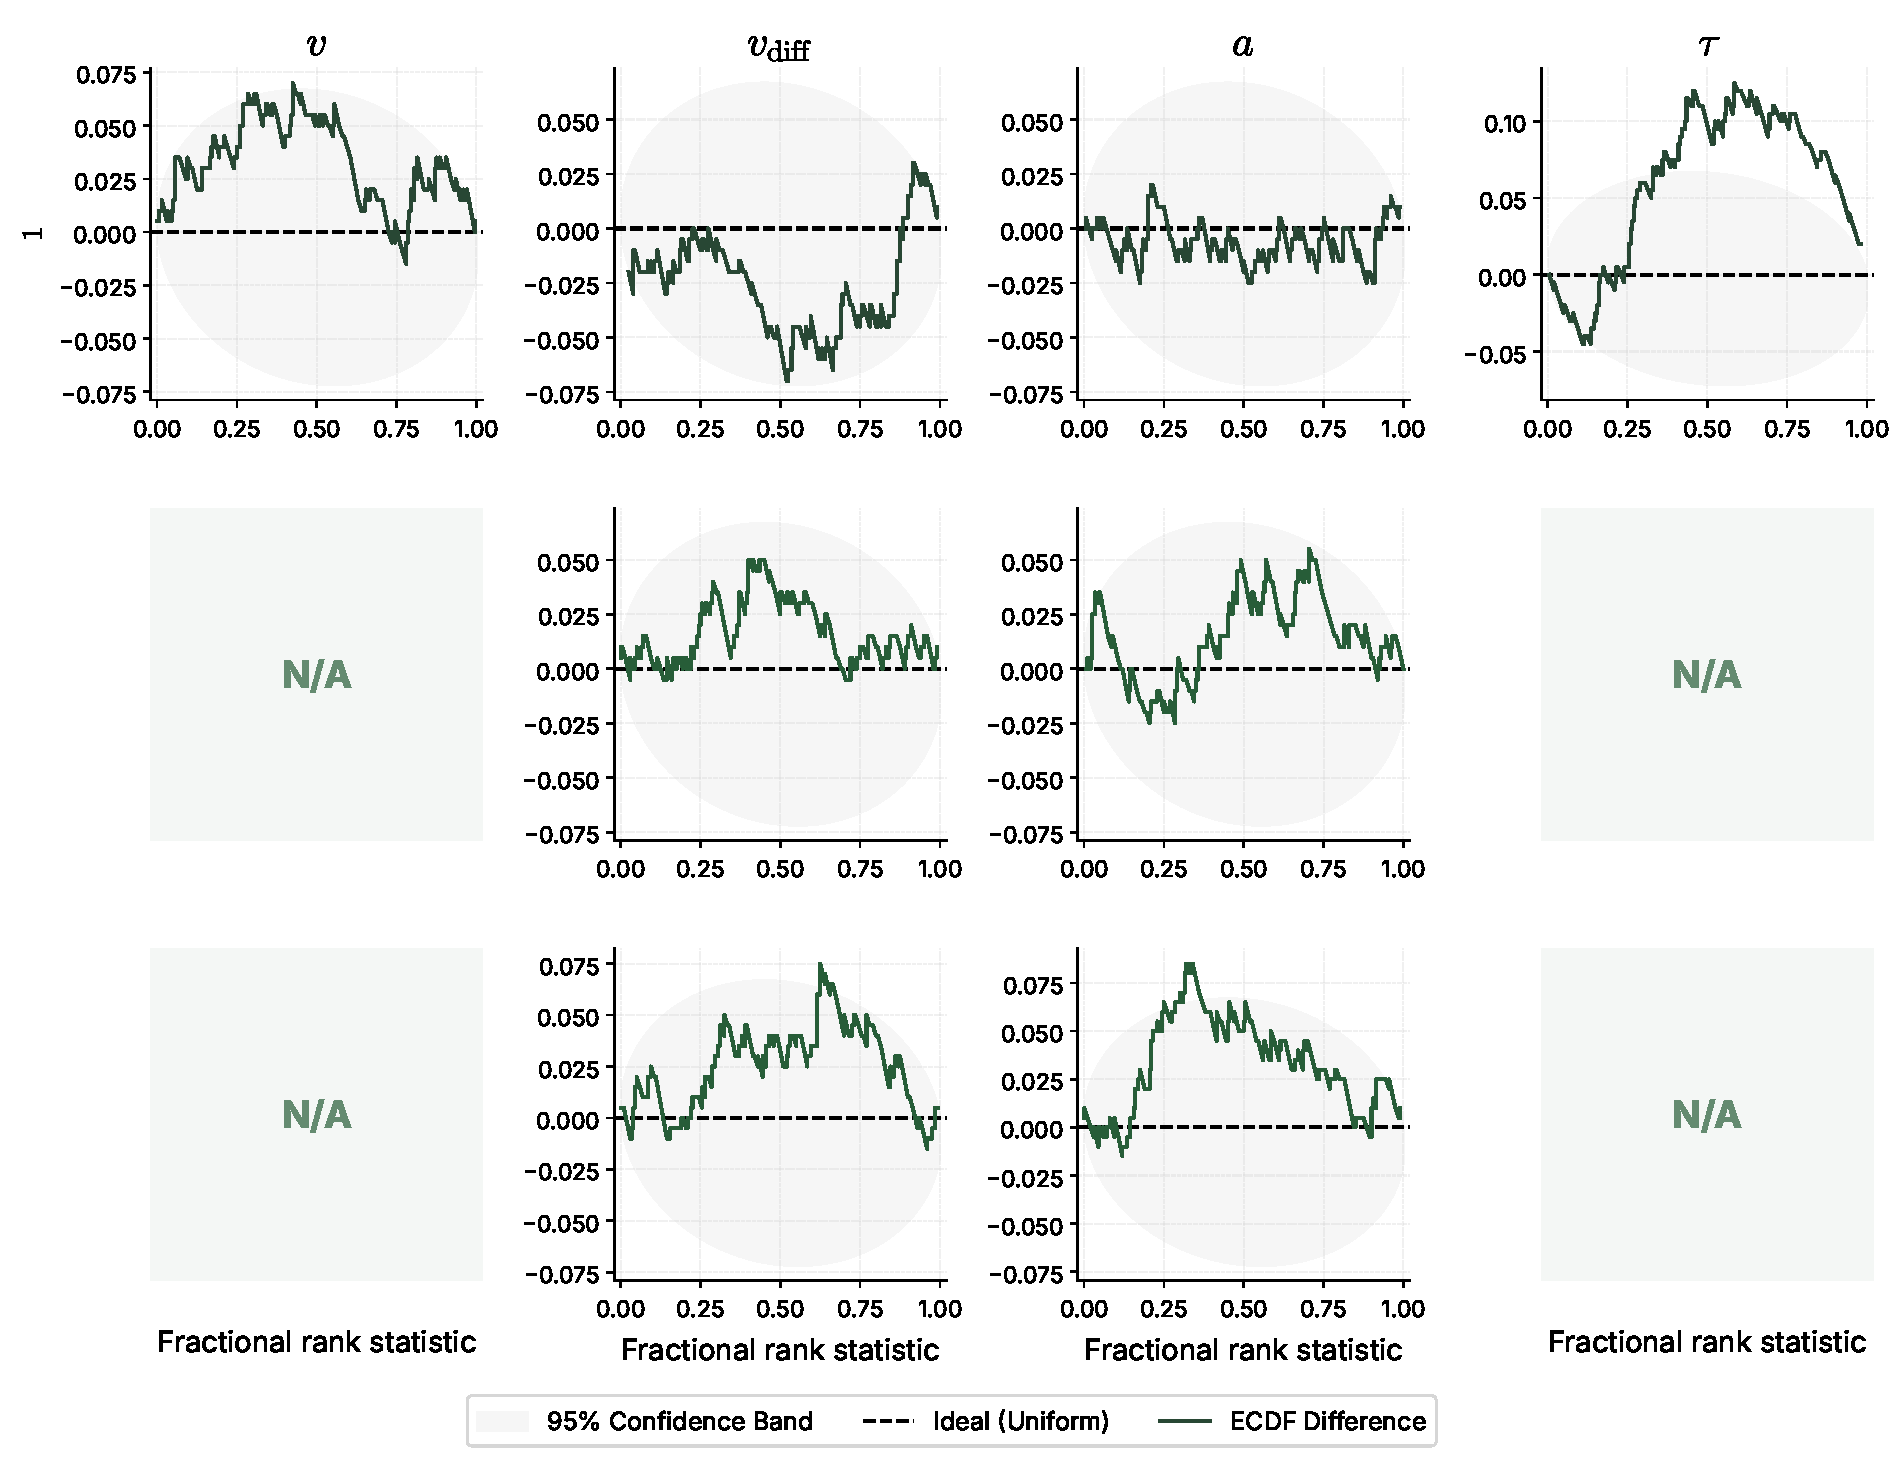
\includegraphics[width=\textwidth,height=0.3\textheight,keepaspectratio]{rdm/fixed_regressed/bf_ecdf.pdf}\par\vspace{1ex}
  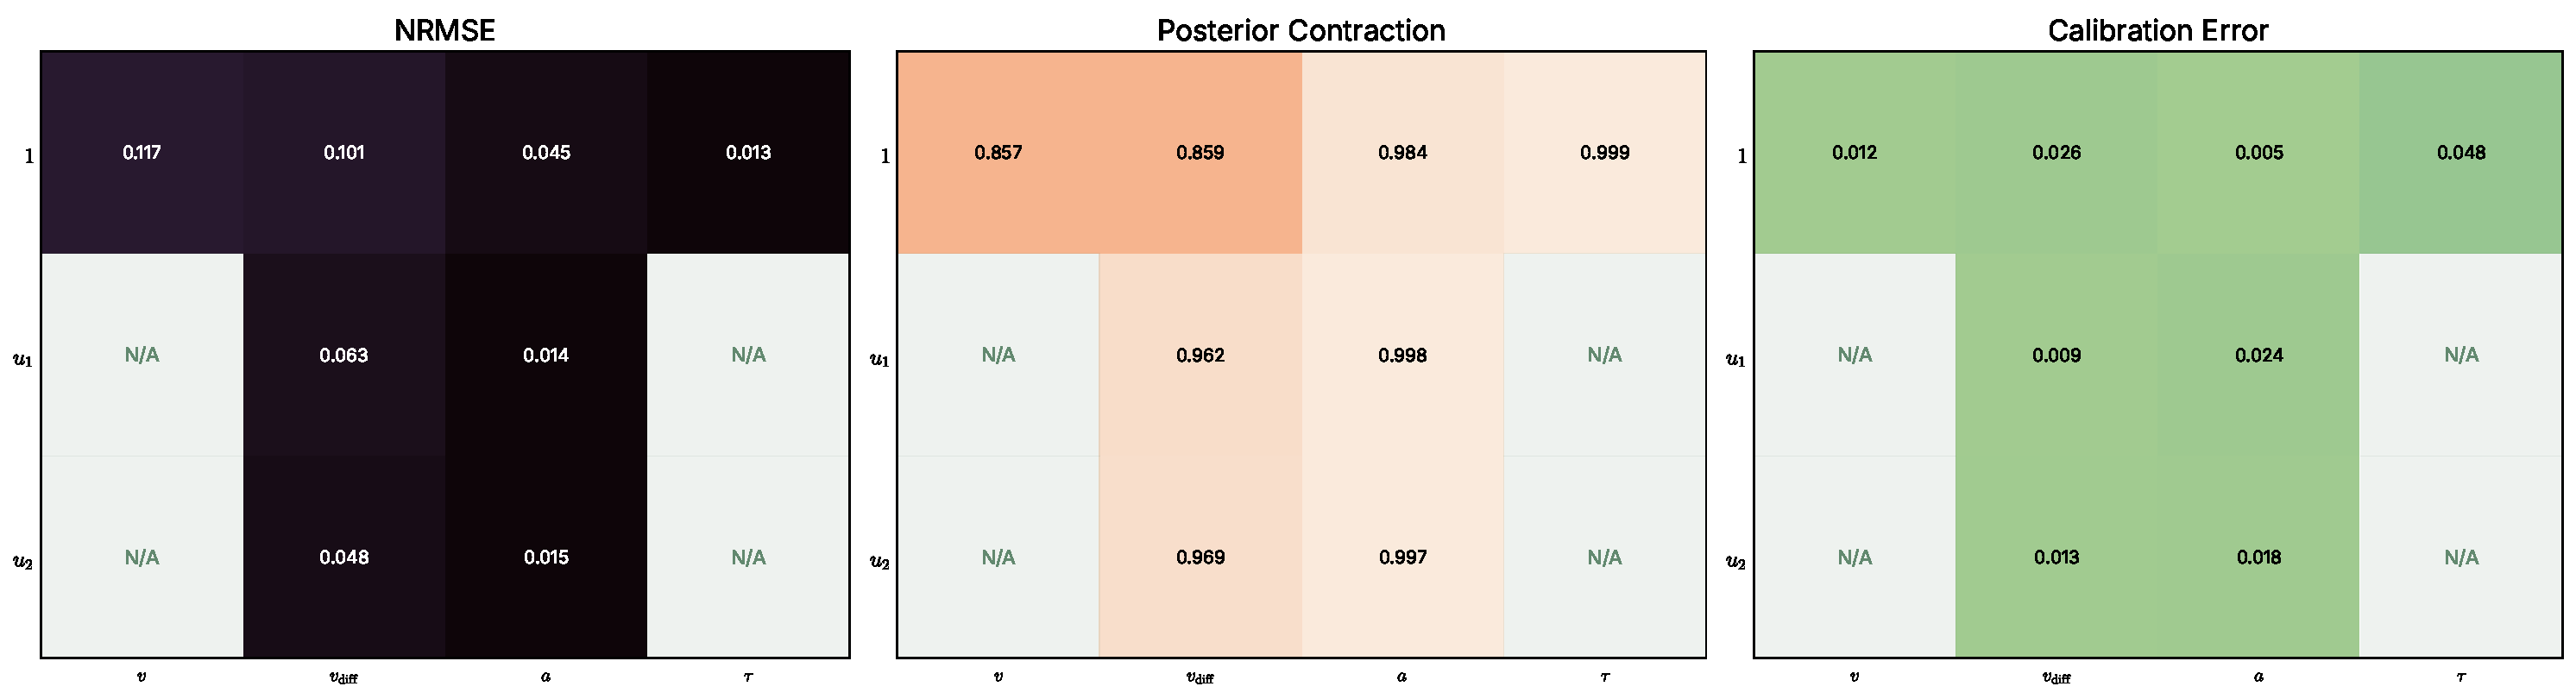
\includegraphics[width=\textwidth]{rdm/fixed_regressed/bf_metrics.pdf}
  \caption{\textbf{RDM, \emph{fixed + regressed} design: BayesFlow baseline.} Recovery (top), calibration (middle), metrics (bottom). $s_v$ and $s_\tau$ are fixed at 0 and not estimated; $v_{\mathrm{diff}}$ and $a$ carry slopes on $u_1$ and $u_2$ (8 coefficients shown). Layout and encoding as in Figure~\ref{fig:app1-ddm-intercept-only-cf}.}
  \label{fig:app1-rdm-fixed-regressed-bf}
\end{figure}

\begin{figure}[p]
  \centering
  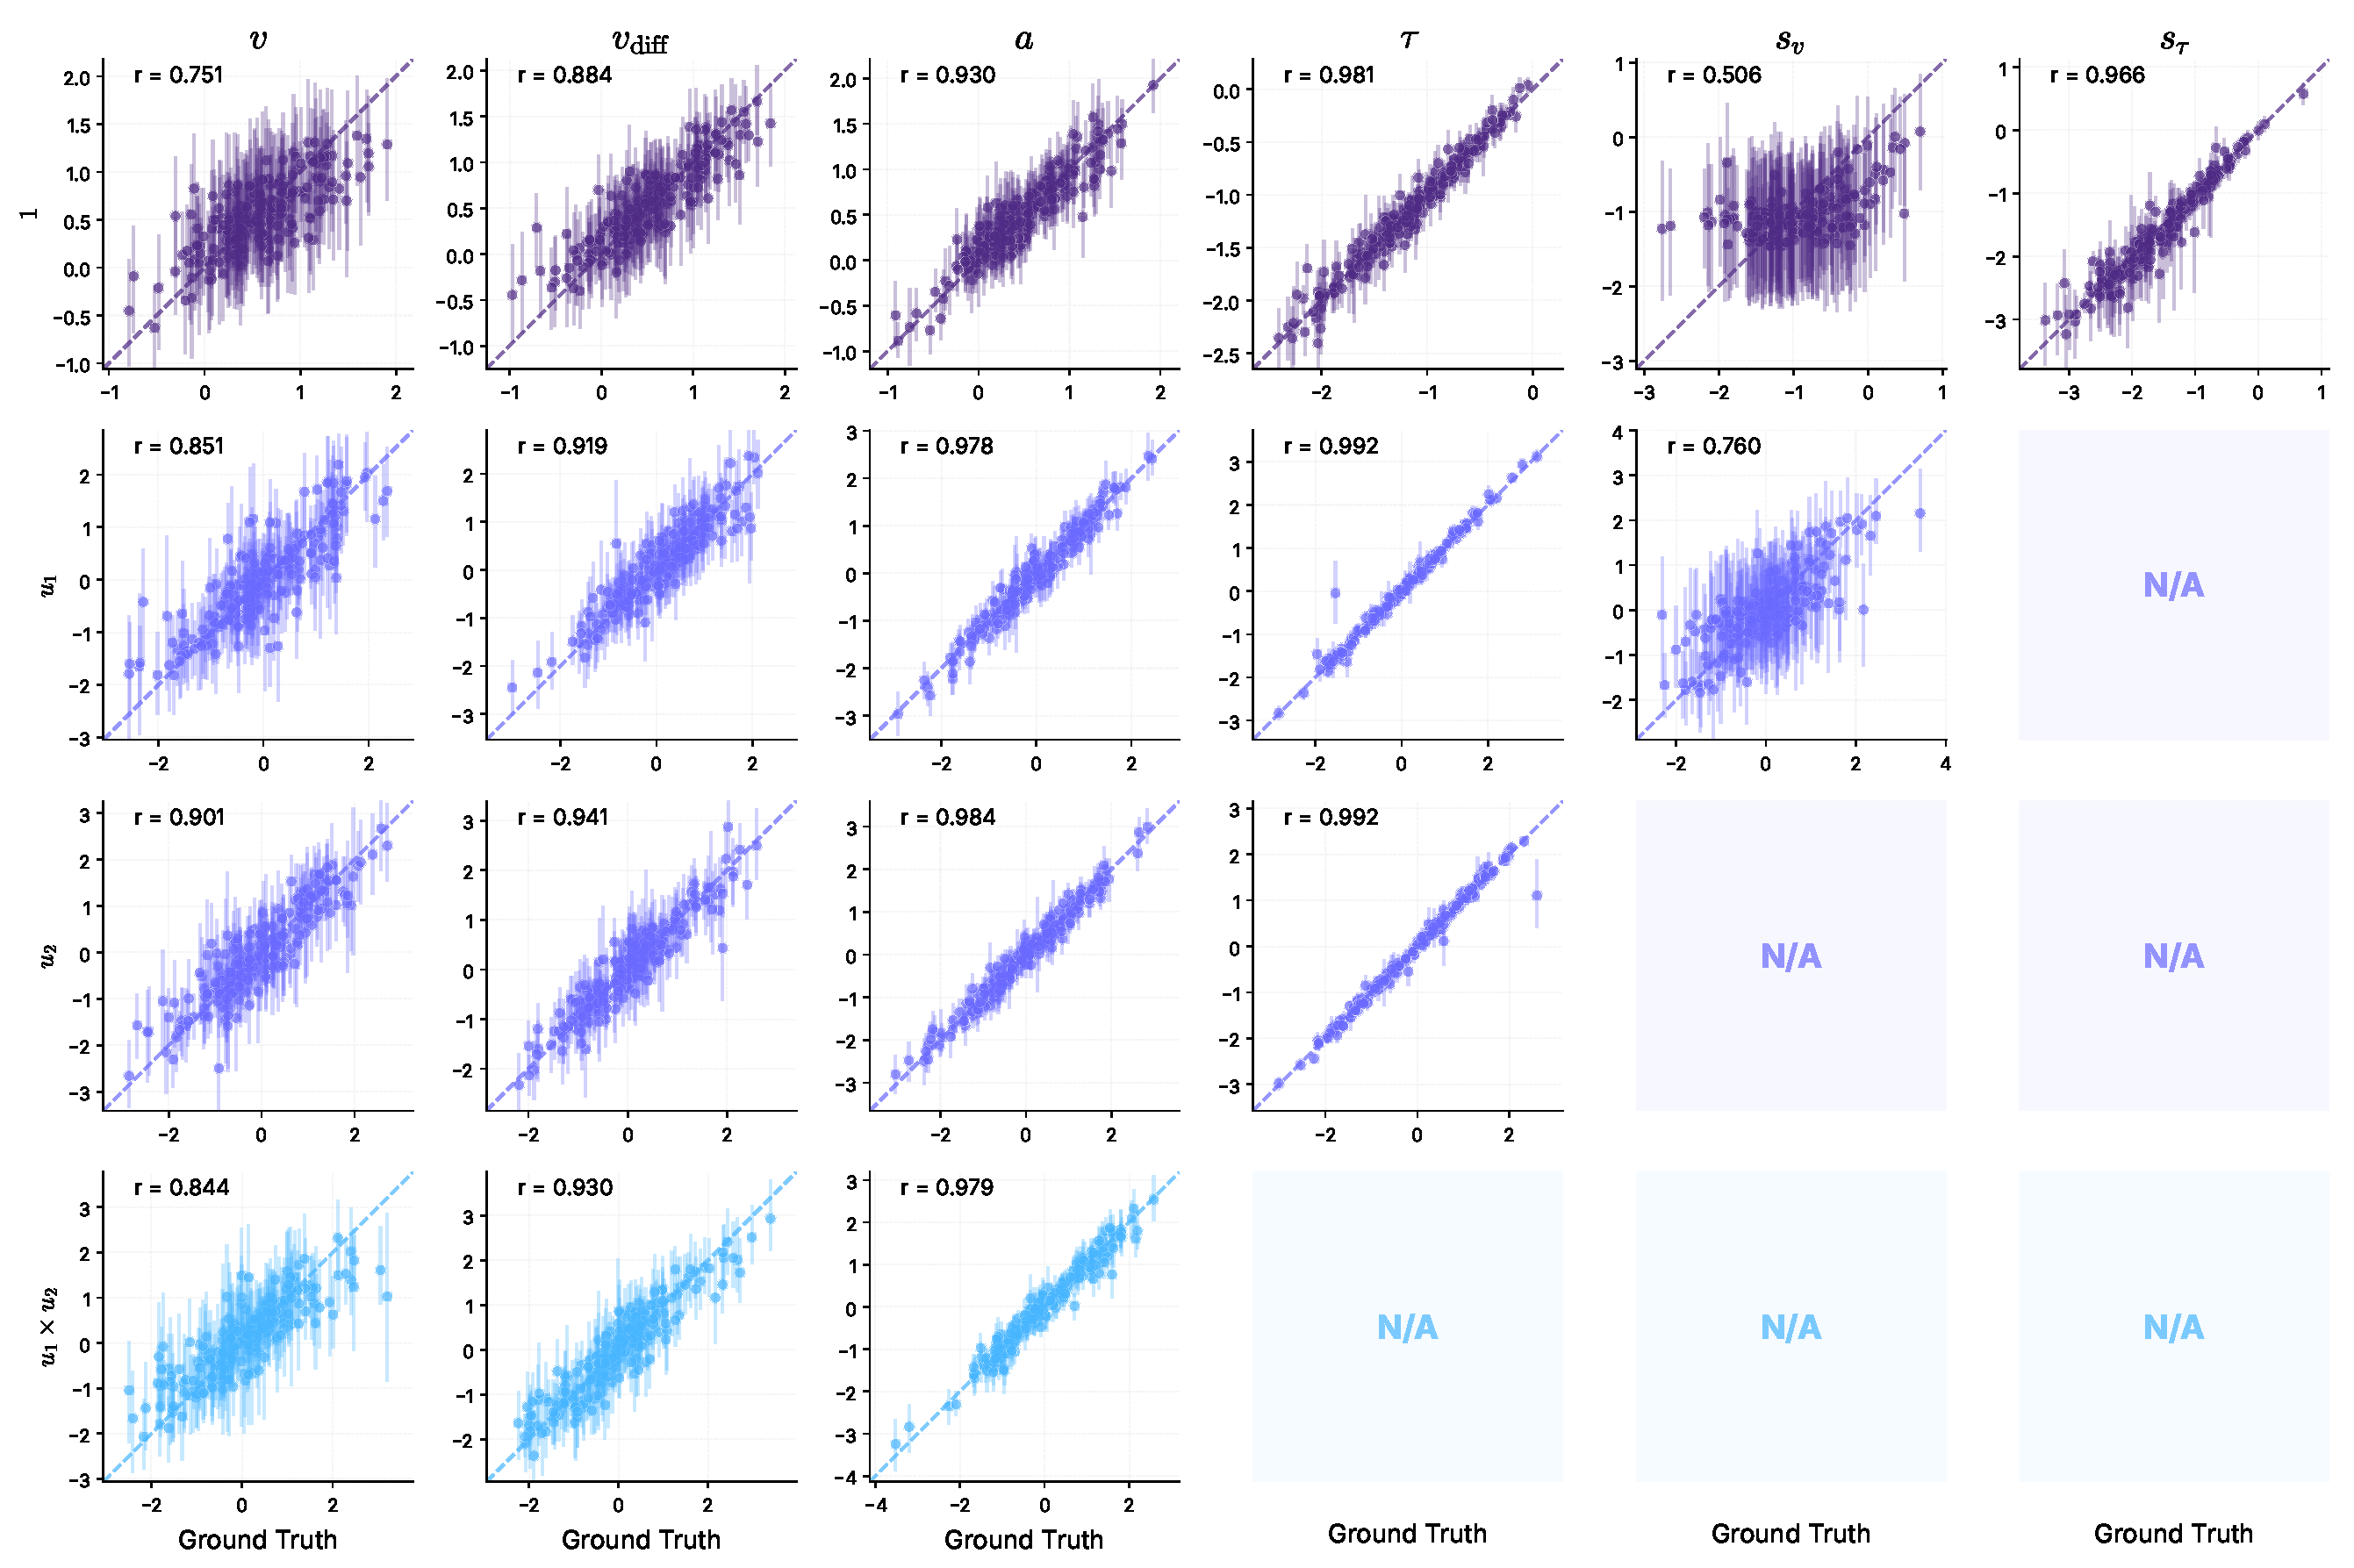
\includegraphics[width=\textwidth,height=0.3\textheight,keepaspectratio]{rdm/interaction/cf_recovery.pdf}\par\vspace{1ex}
  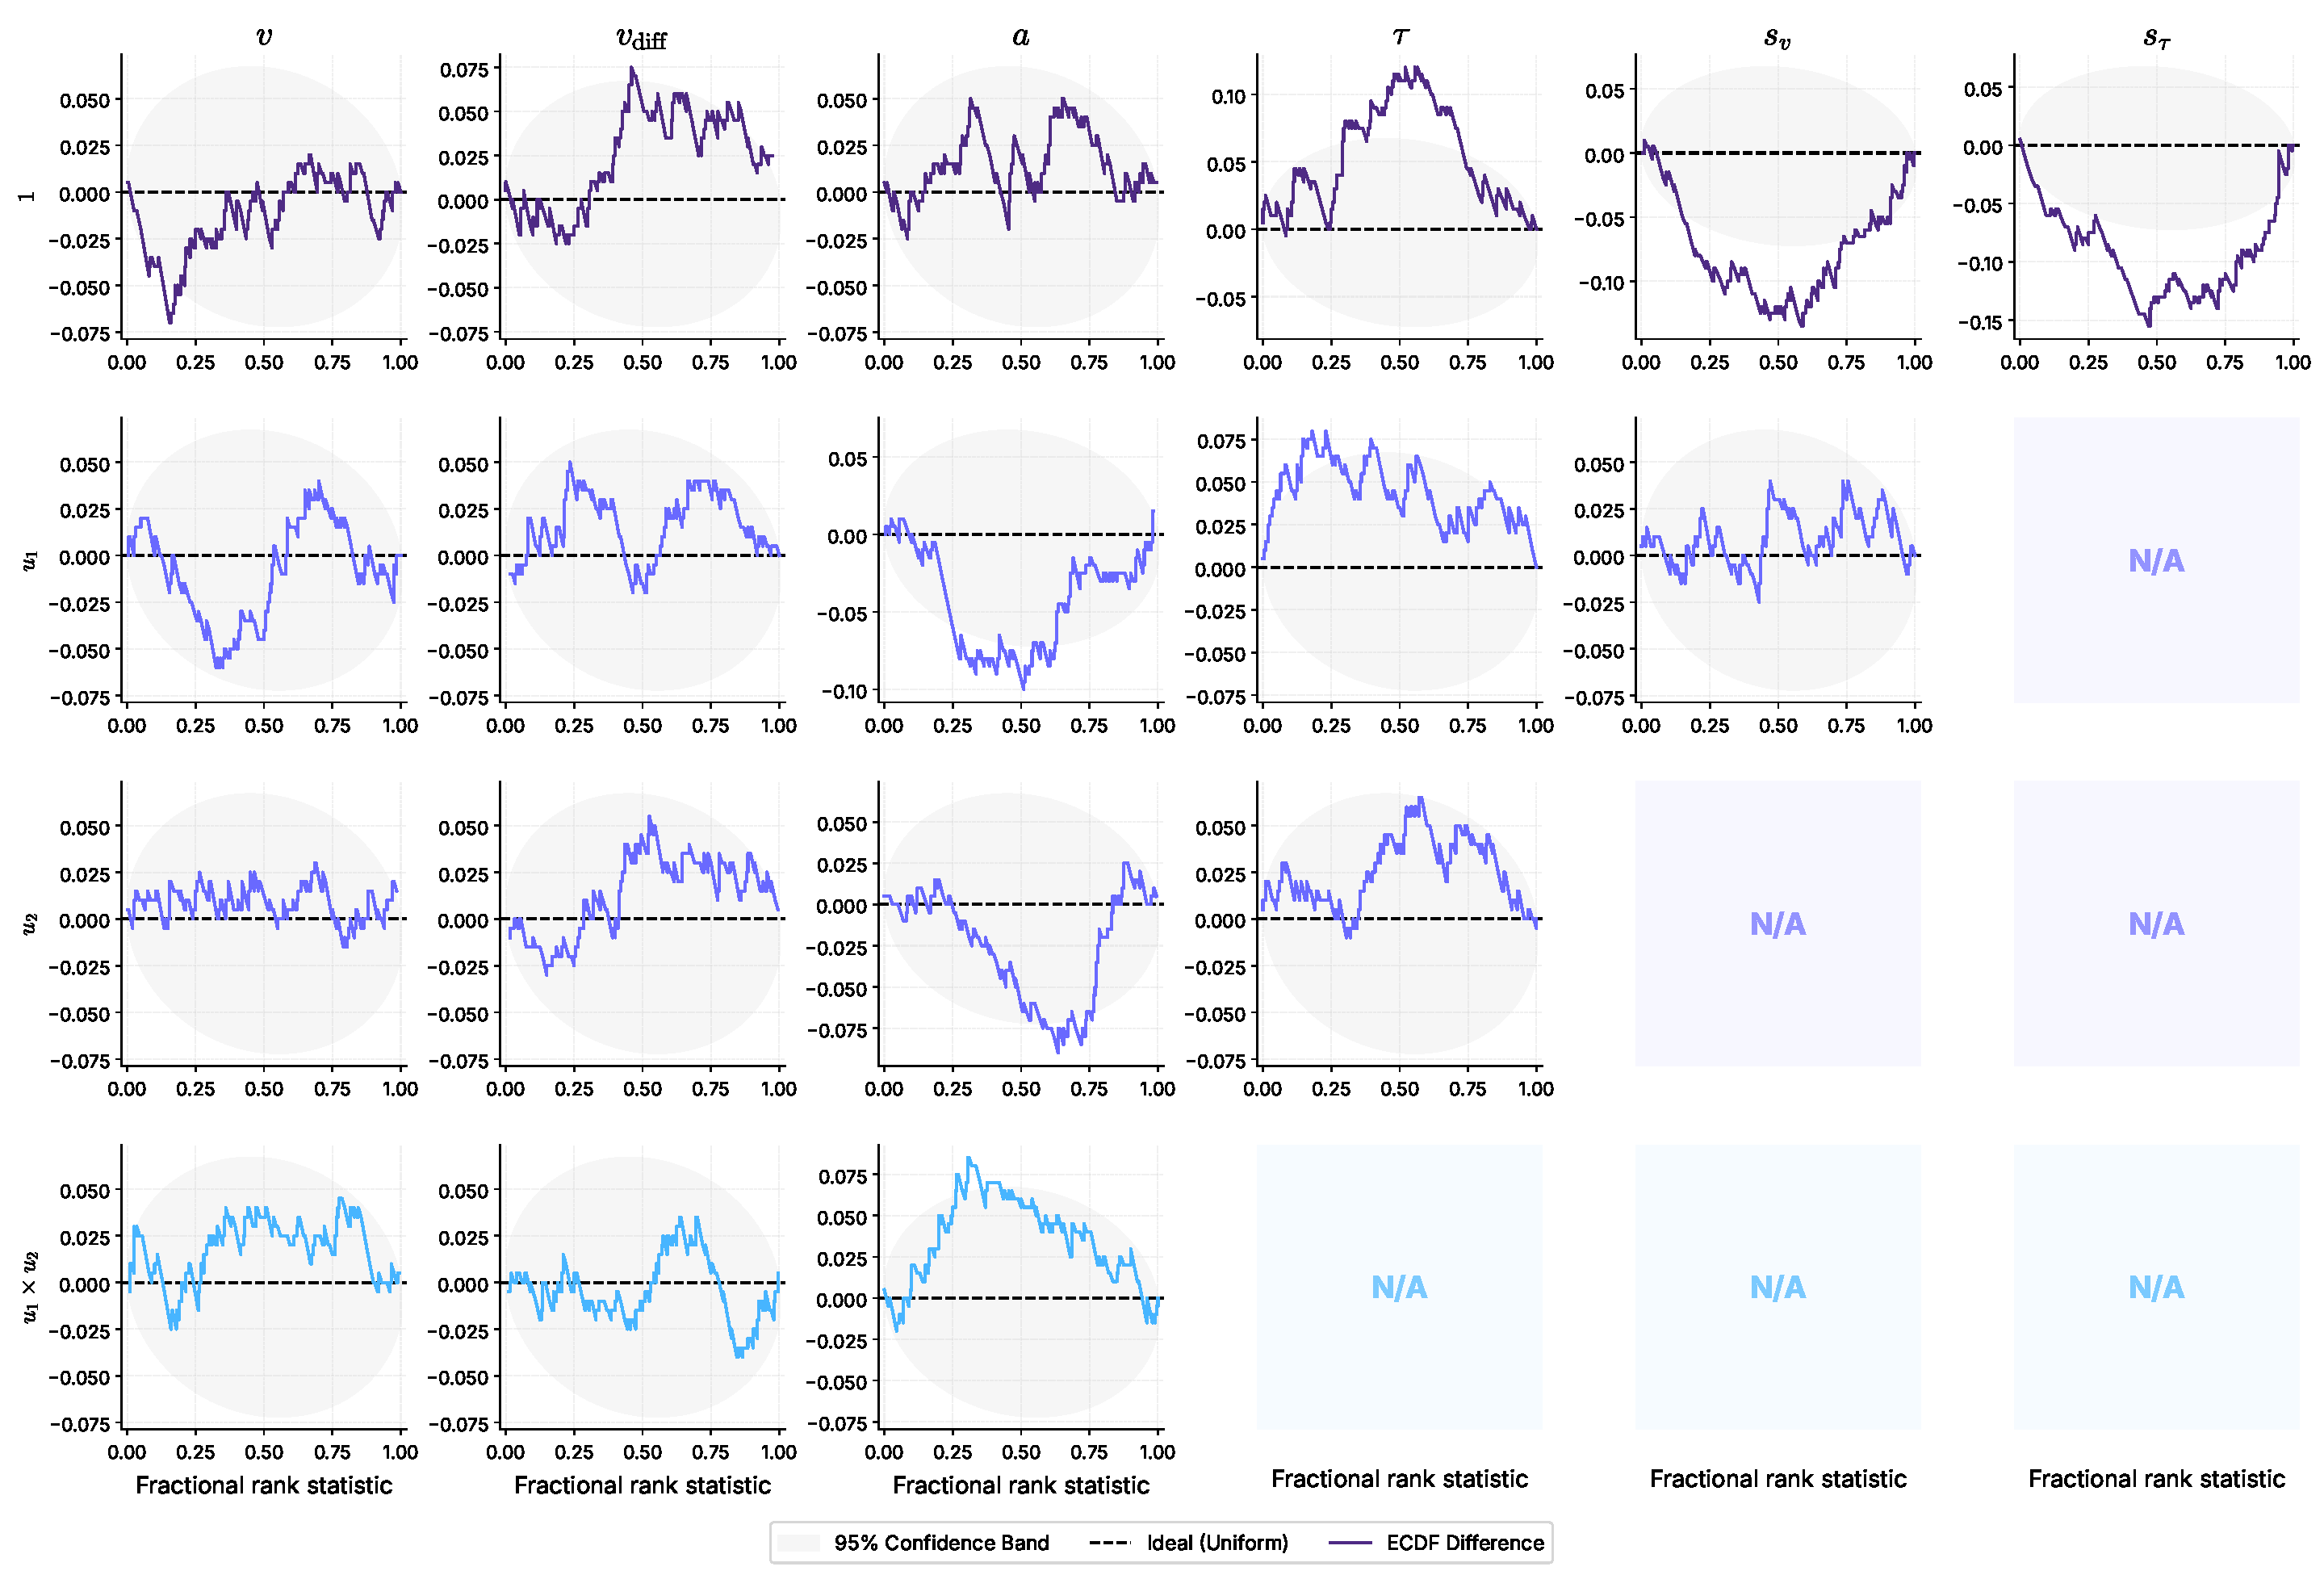
\includegraphics[width=\textwidth,height=0.3\textheight,keepaspectratio]{rdm/interaction/cf_ecdf.pdf}\par\vspace{1ex}
  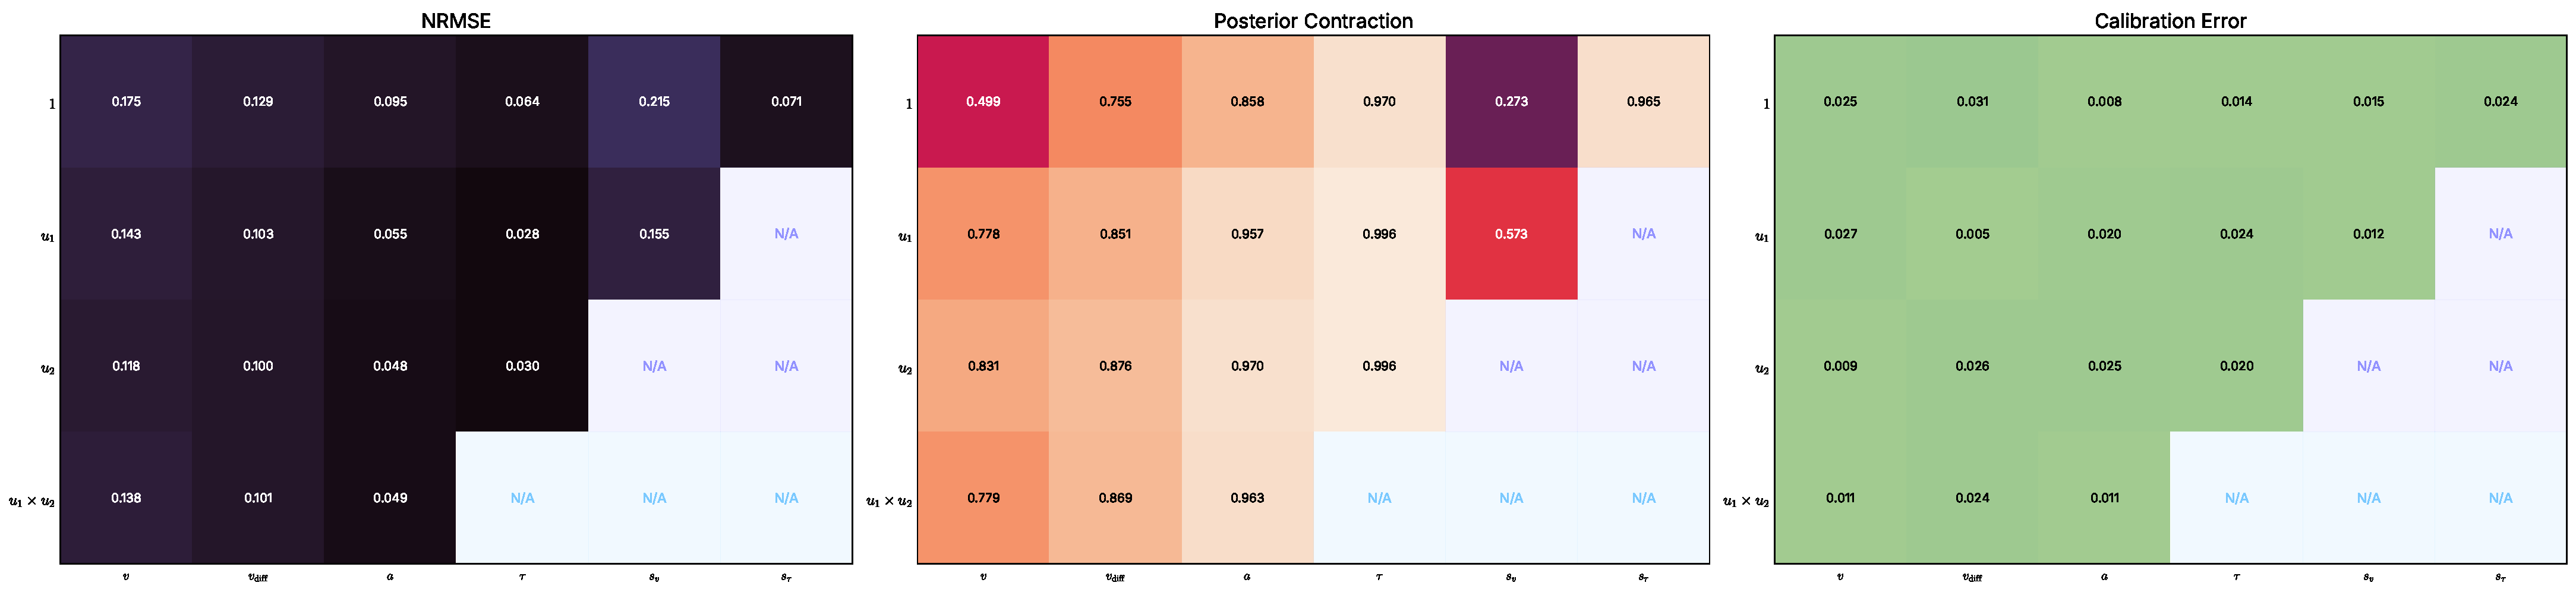
\includegraphics[width=\textwidth]{rdm/interaction/cf_metrics.pdf}
  \caption{\textbf{RDM, \emph{interaction} design: CogFormer.} Recovery (top), calibration (middle), metrics (bottom). $v$, $v_{\mathrm{diff}}$, $a$, $\tau$ and $s_v$ carry slopes on $u_1$; $v$, $v_{\mathrm{diff}}$, $a$ and $\tau$ carry slopes on $u_2$; $v$, $v_{\mathrm{diff}}$ and $a$ on the product $u_1 u_2$ (18 coefficients shown). Layout and encoding as in Figure~\ref{fig:app1-ddm-intercept-only-cf}.}
  \label{fig:app1-rdm-interaction-cf}
\end{figure}

\begin{figure}[p]
  \centering
  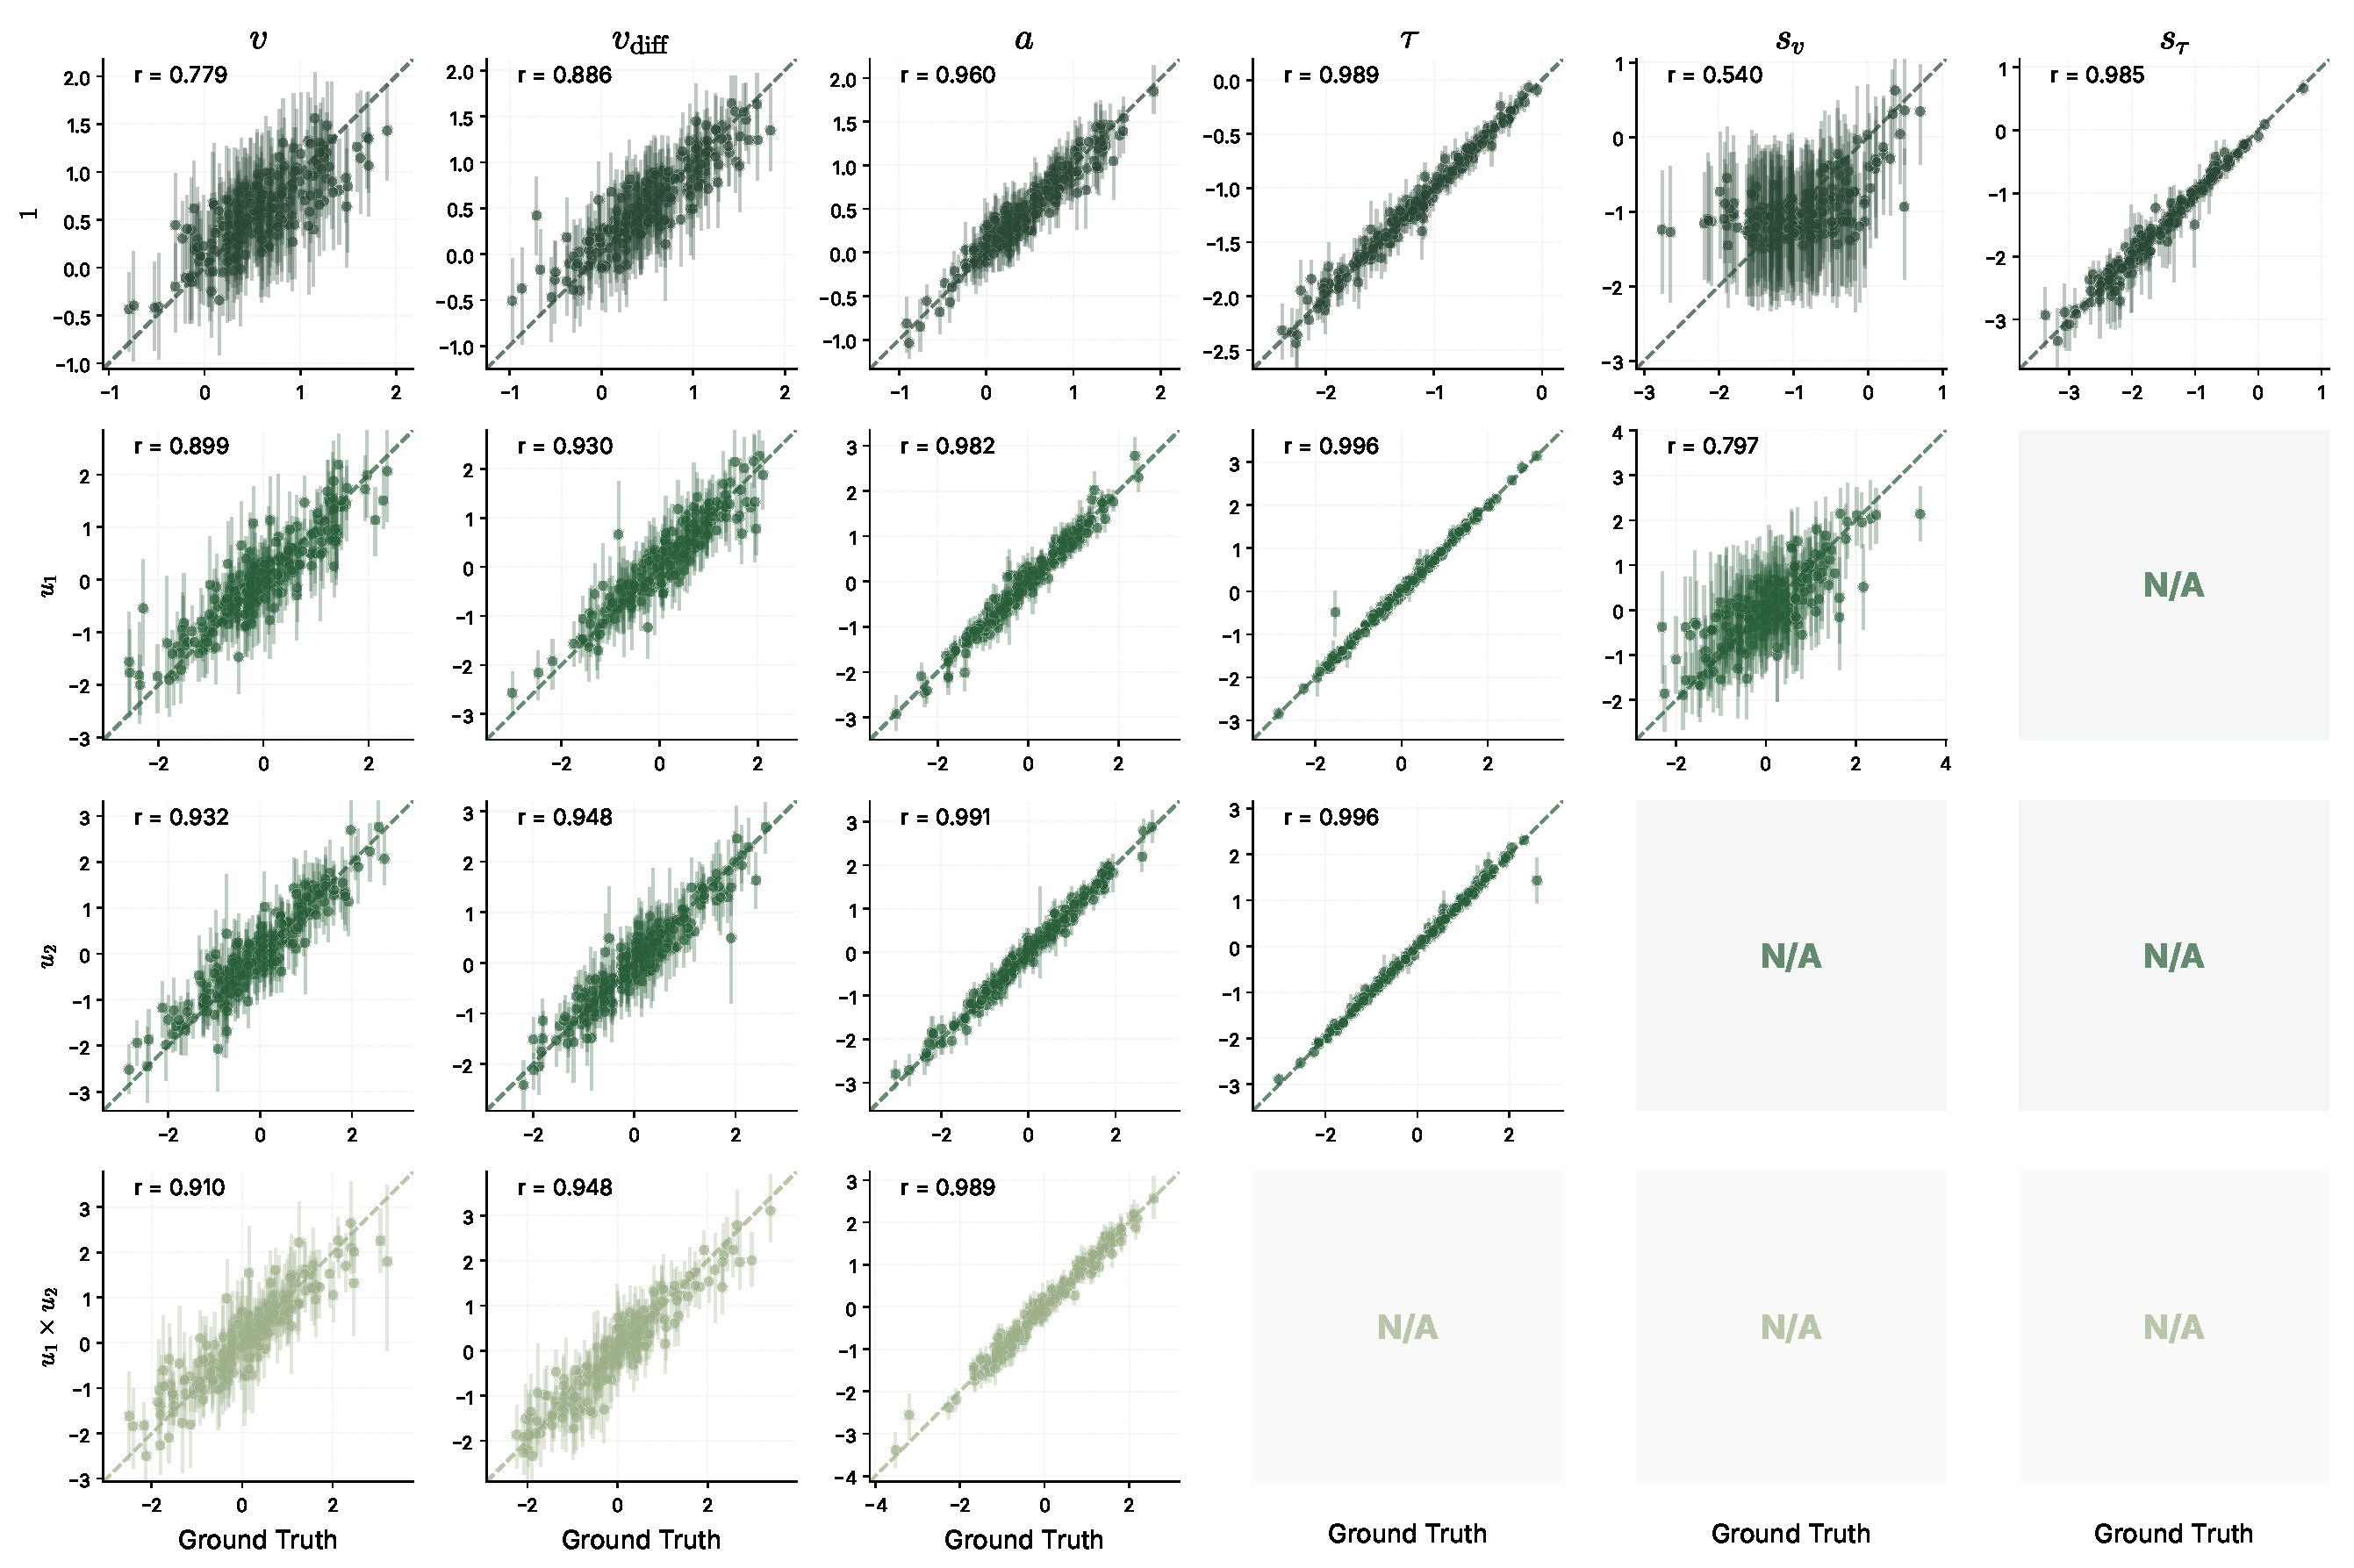
\includegraphics[width=\textwidth,height=0.3\textheight,keepaspectratio]{rdm/interaction/bf_recovery.pdf}\par\vspace{1ex}
  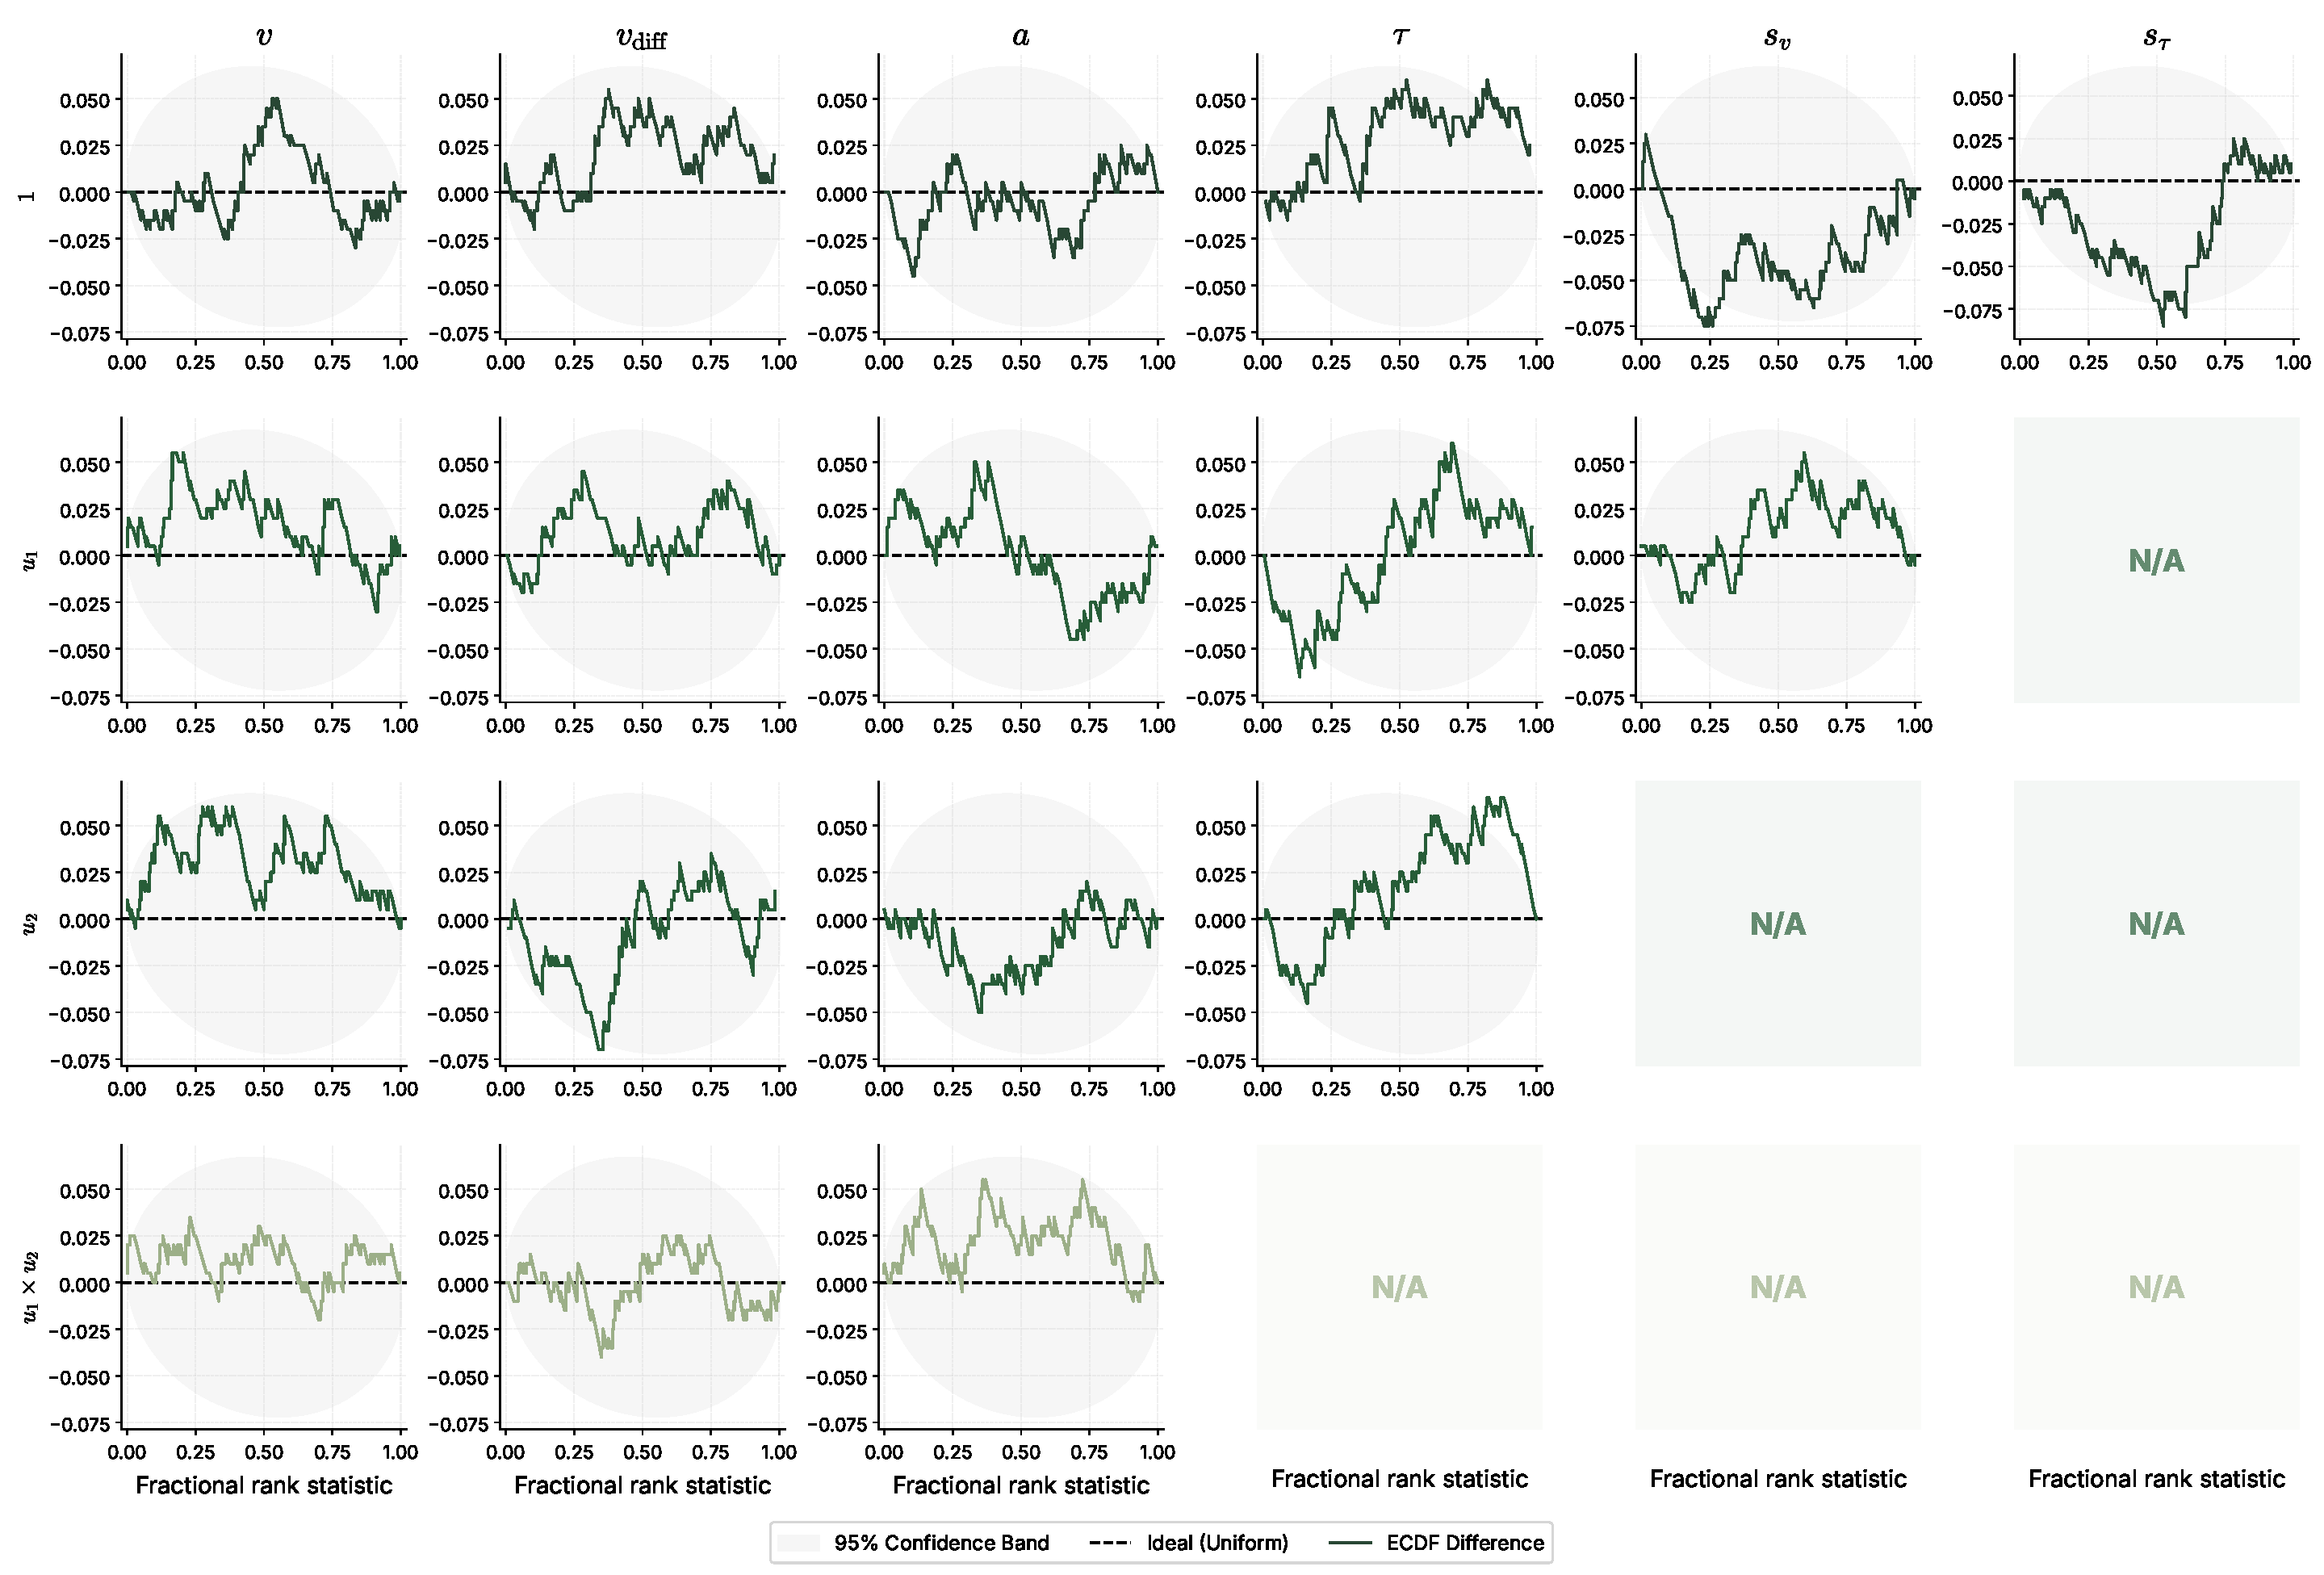
\includegraphics[width=\textwidth,height=0.3\textheight,keepaspectratio]{rdm/interaction/bf_ecdf.pdf}\par\vspace{1ex}
  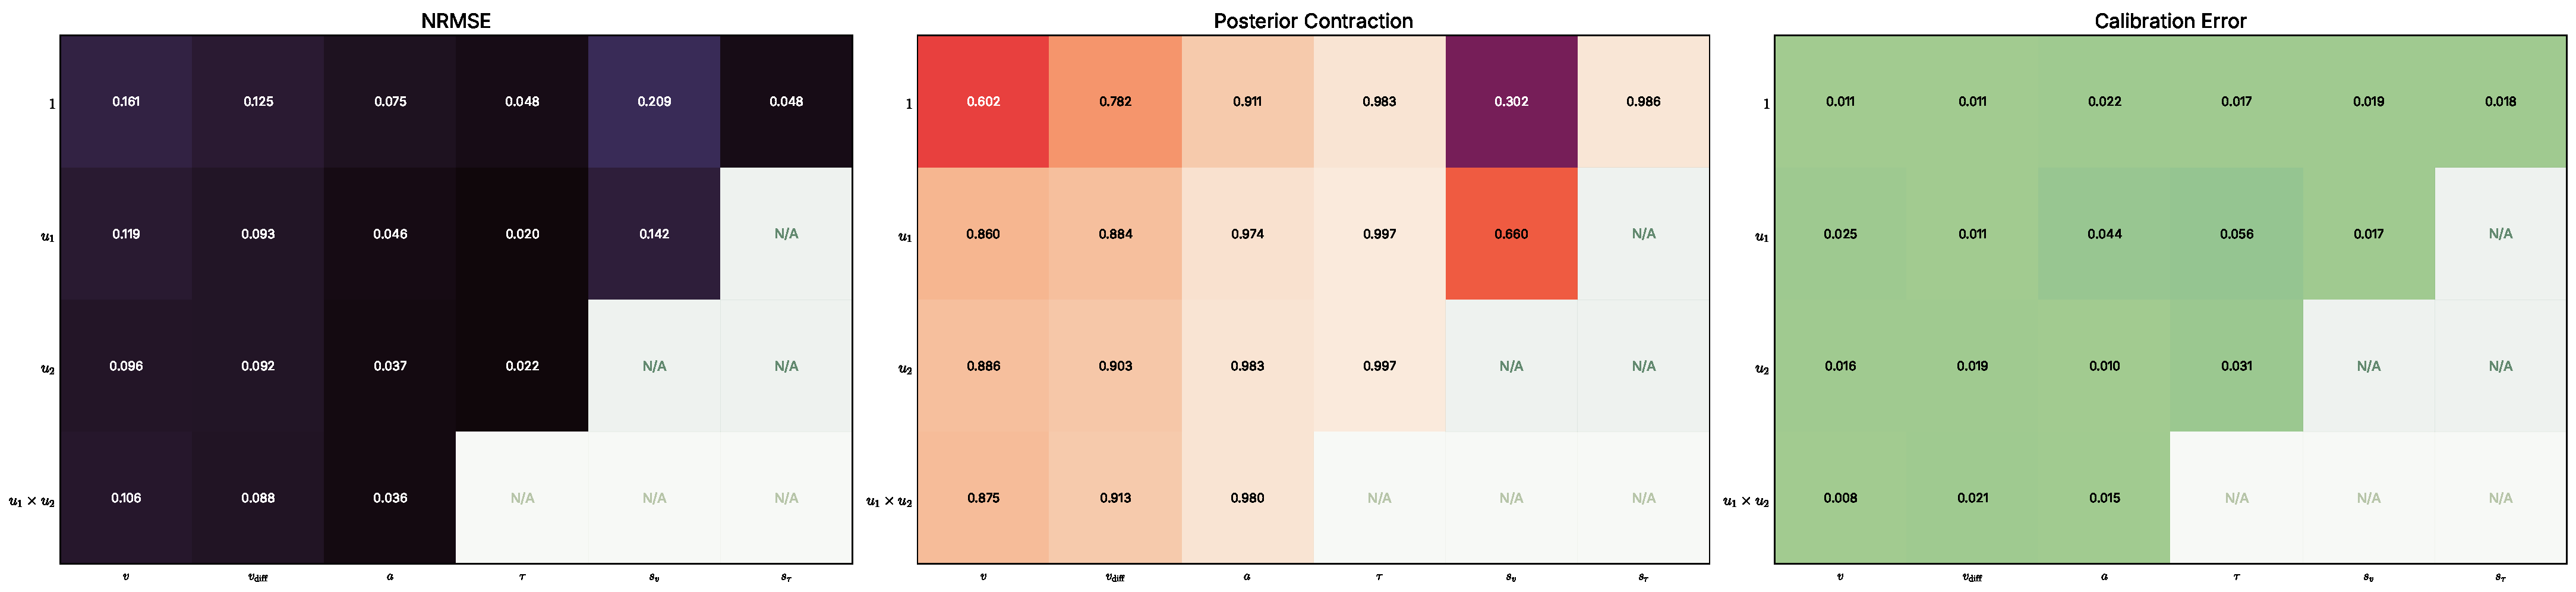
\includegraphics[width=\textwidth]{rdm/interaction/bf_metrics.pdf}
  \caption{\textbf{RDM, \emph{interaction} design: BayesFlow baseline.} Recovery (top), calibration (middle), metrics (bottom). $v$, $v_{\mathrm{diff}}$, $a$, $\tau$ and $s_v$ carry slopes on $u_1$; $v$, $v_{\mathrm{diff}}$, $a$ and $\tau$ carry slopes on $u_2$; $v$, $v_{\mathrm{diff}}$ and $a$ on the product $u_1 u_2$ (18 coefficients shown). Layout and encoding as in Figure~\ref{fig:app1-ddm-intercept-only-cf}.}
  \label{fig:app1-rdm-interaction-bf}
\end{figure}

\begin{figure}[p]
  \centering
  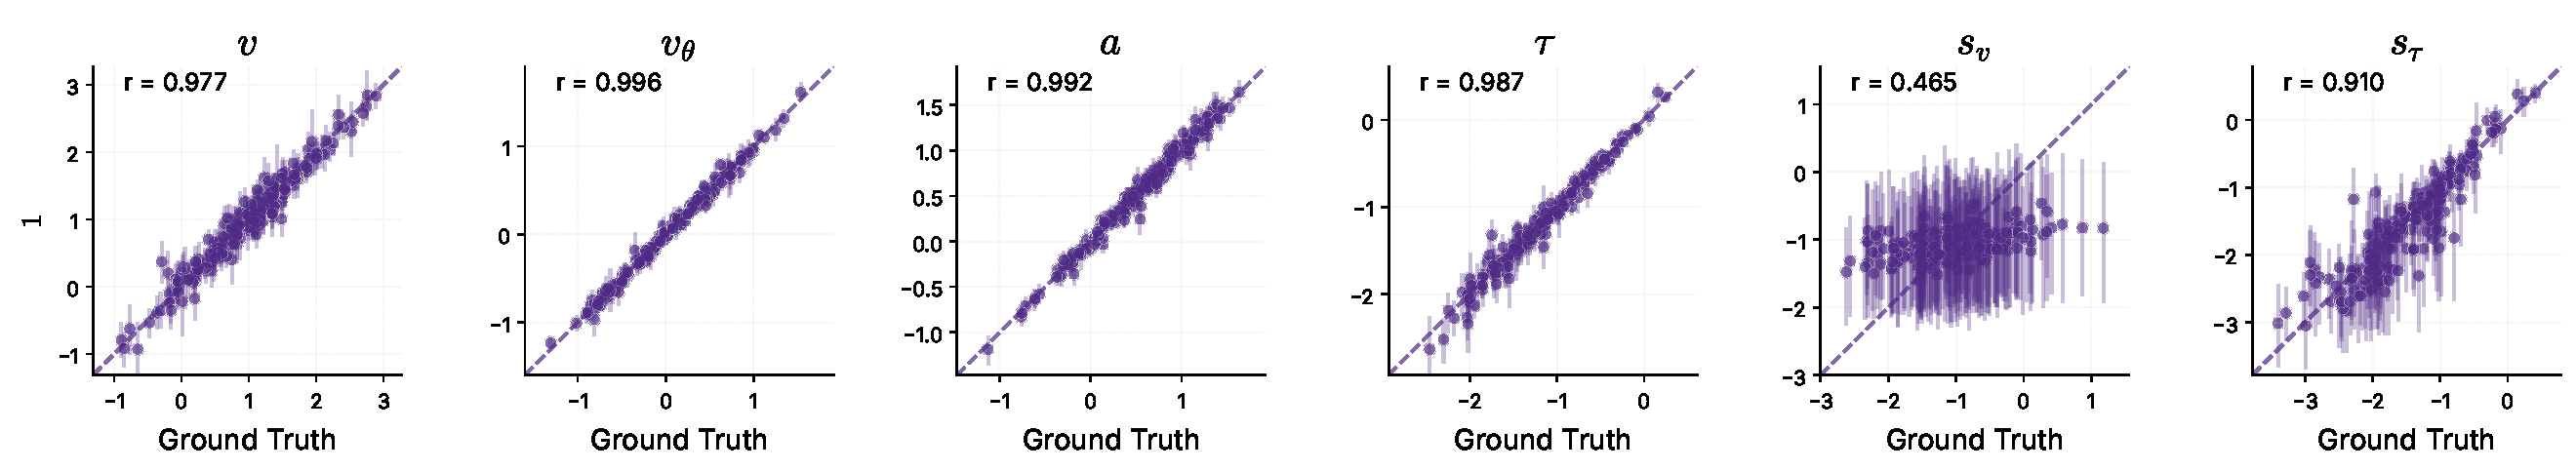
\includegraphics[width=\textwidth,height=0.3\textheight,keepaspectratio]{cdm/intercept_only/cf_recovery.pdf}\par\vspace{1ex}
  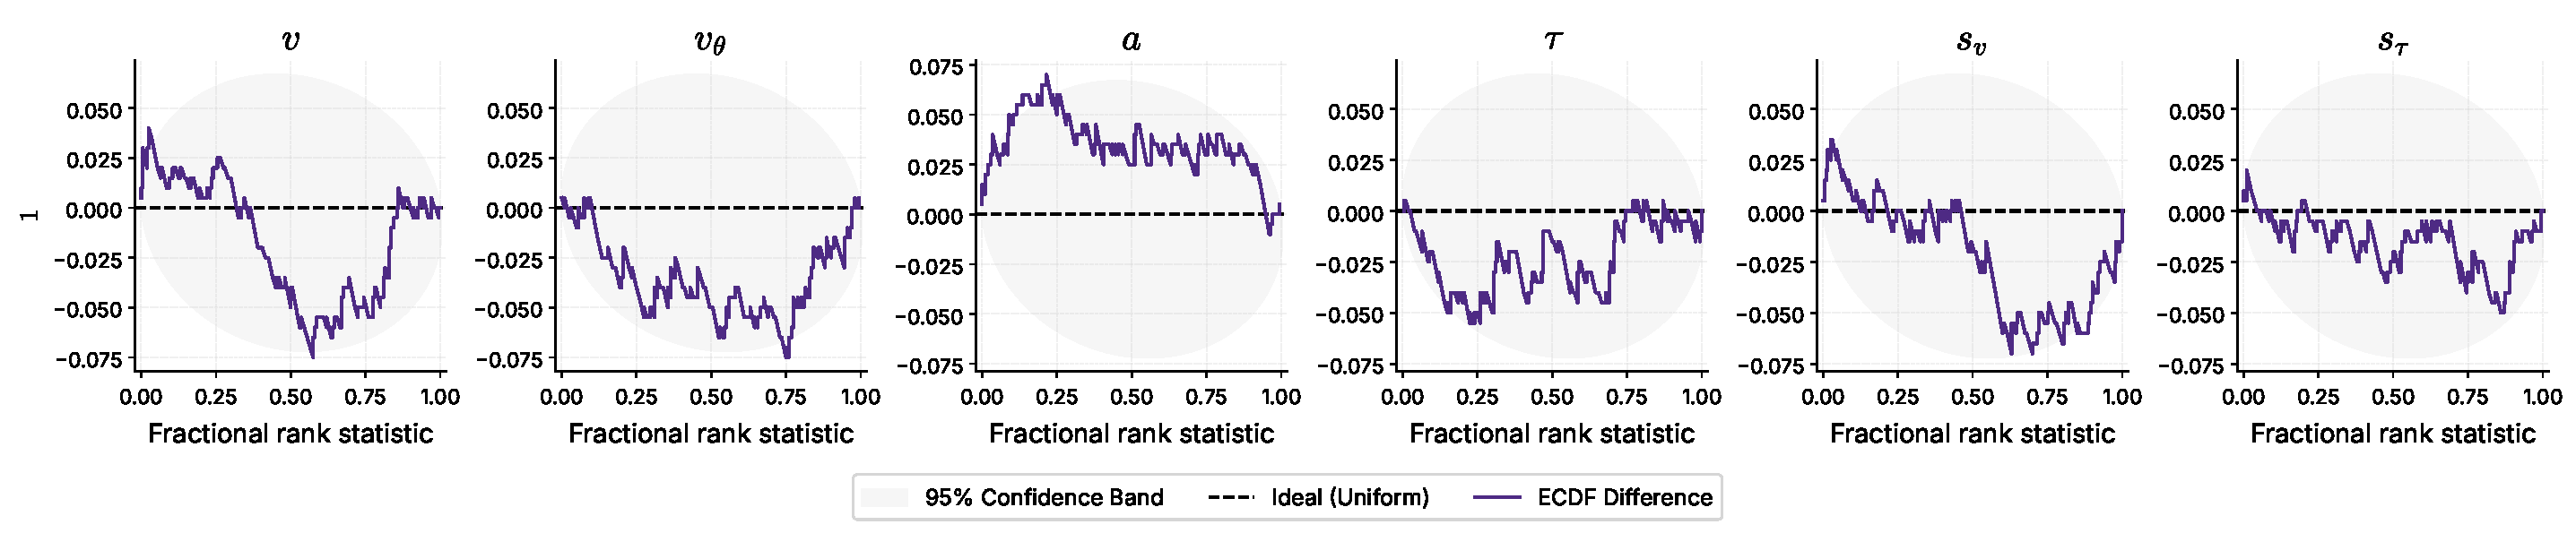
\includegraphics[width=\textwidth,height=0.3\textheight,keepaspectratio]{cdm/intercept_only/cf_ecdf.pdf}\par\vspace{1ex}
  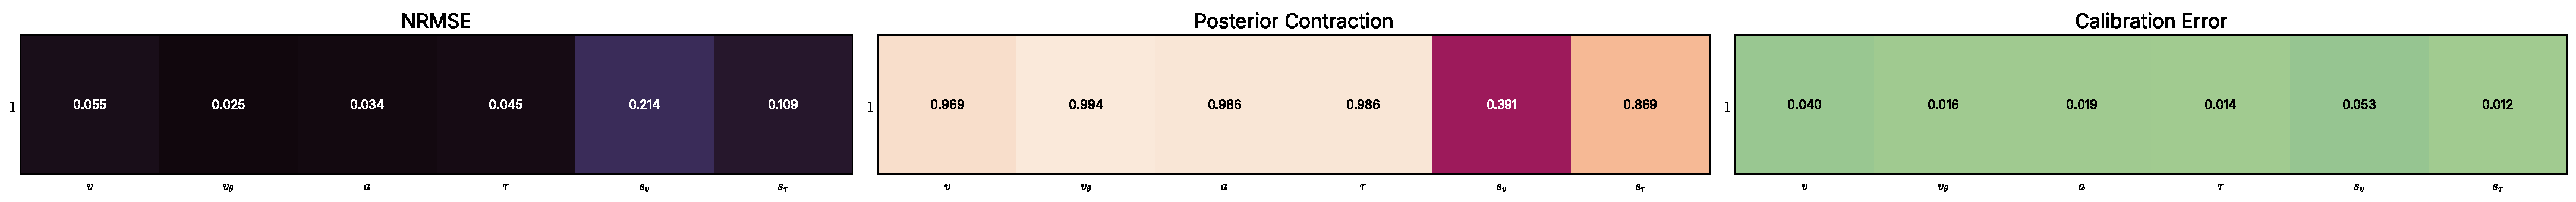
\includegraphics[width=\textwidth]{cdm/intercept_only/cf_metrics.pdf}
  \caption{\textbf{CDM, \emph{intercept-only} design: CogFormer.} Recovery (top), calibration (middle), metrics (bottom). Every estimated parameter enters as an intercept only (6 coefficients shown). Layout and encoding as in Figure~\ref{fig:app1-ddm-intercept-only-cf}.}
  \label{fig:app1-cdm-intercept-only-cf}
\end{figure}

\begin{figure}[p]
  \centering
  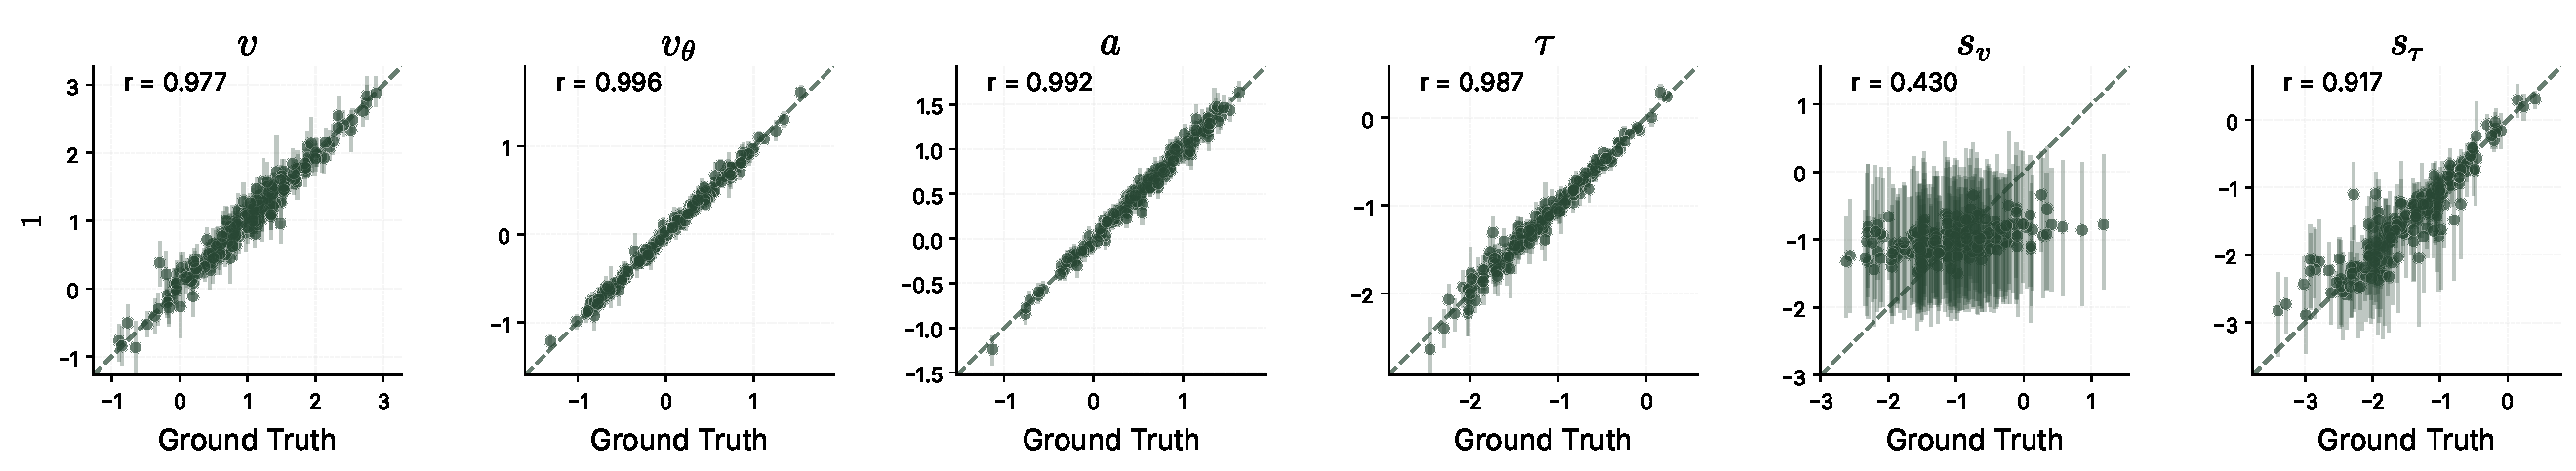
\includegraphics[width=\textwidth,height=0.3\textheight,keepaspectratio]{cdm/intercept_only/bf_recovery.pdf}\par\vspace{1ex}
  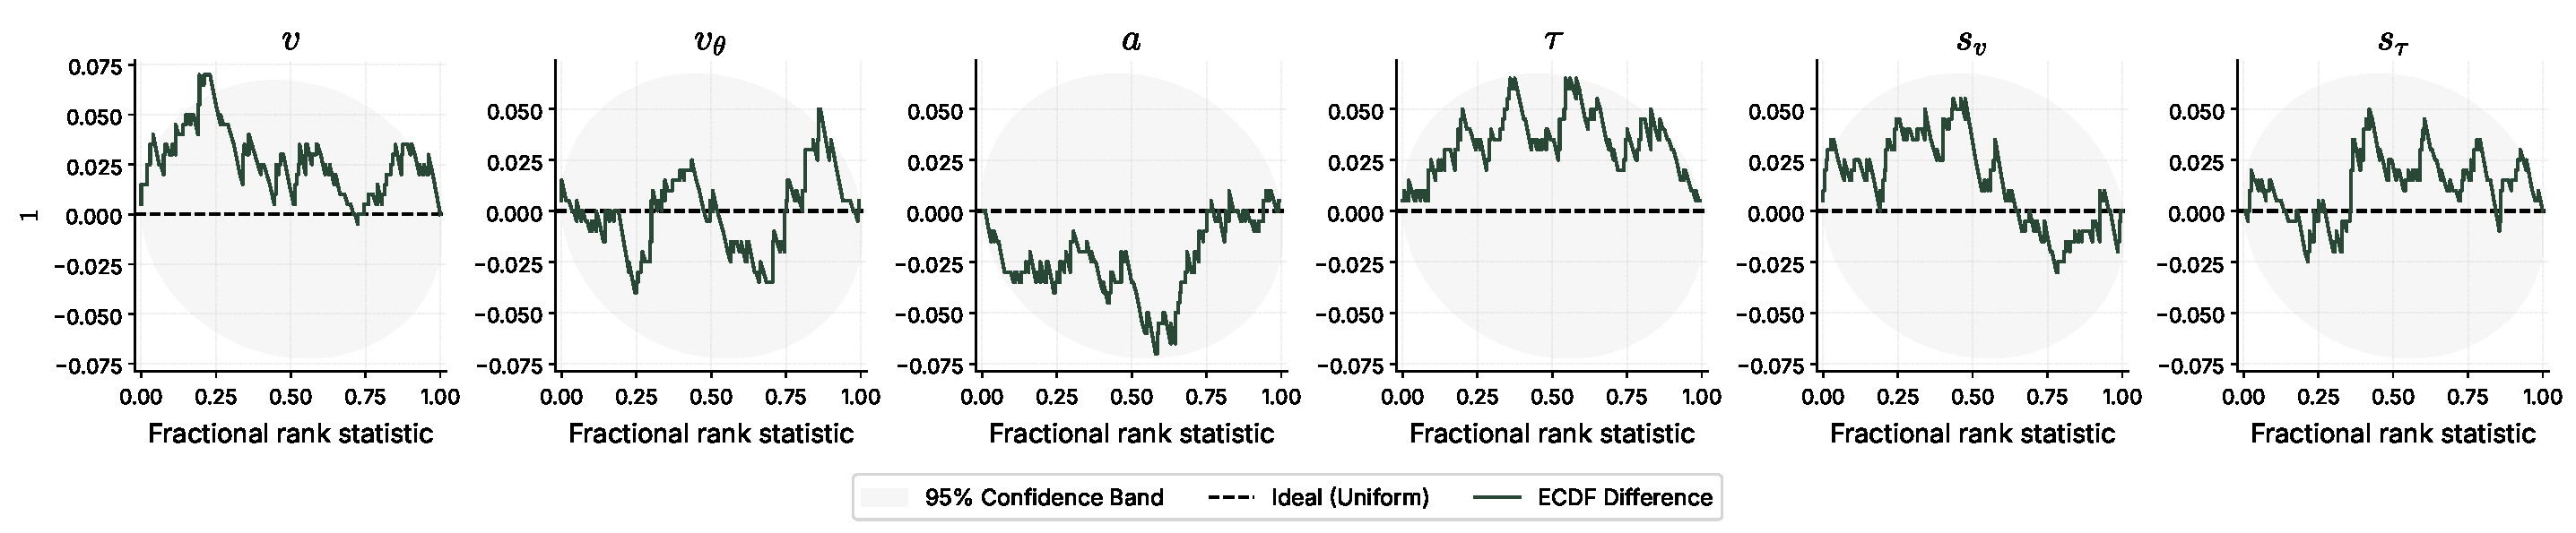
\includegraphics[width=\textwidth,height=0.3\textheight,keepaspectratio]{cdm/intercept_only/bf_ecdf.pdf}\par\vspace{1ex}
  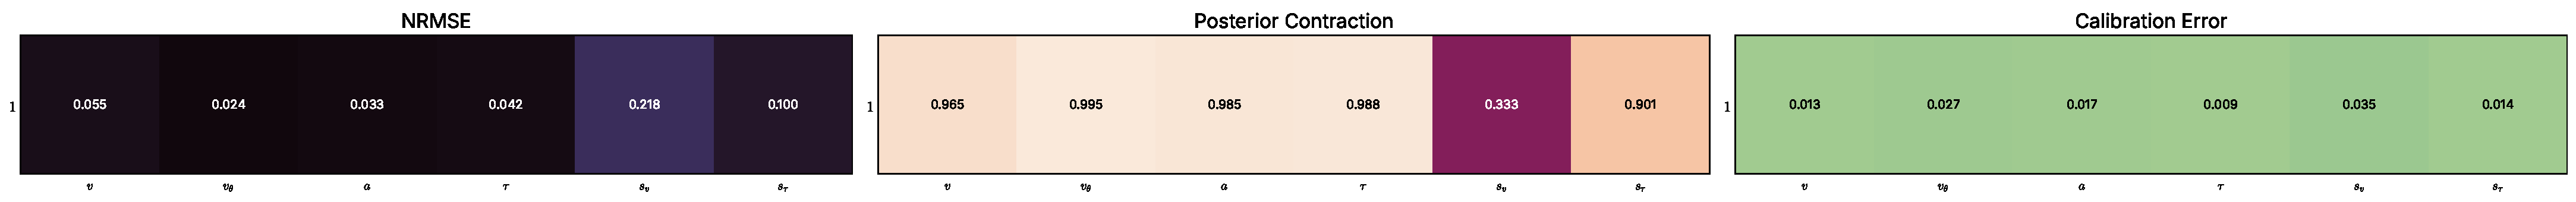
\includegraphics[width=\textwidth]{cdm/intercept_only/bf_metrics.pdf}
  \caption{\textbf{CDM, \emph{intercept-only} design: BayesFlow baseline.} Recovery (top), calibration (middle), metrics (bottom). Every estimated parameter enters as an intercept only (6 coefficients shown). Layout and encoding as in Figure~\ref{fig:app1-ddm-intercept-only-cf}.}
  \label{fig:app1-cdm-intercept-only-bf}
\end{figure}

\begin{figure}[p]
  \centering
  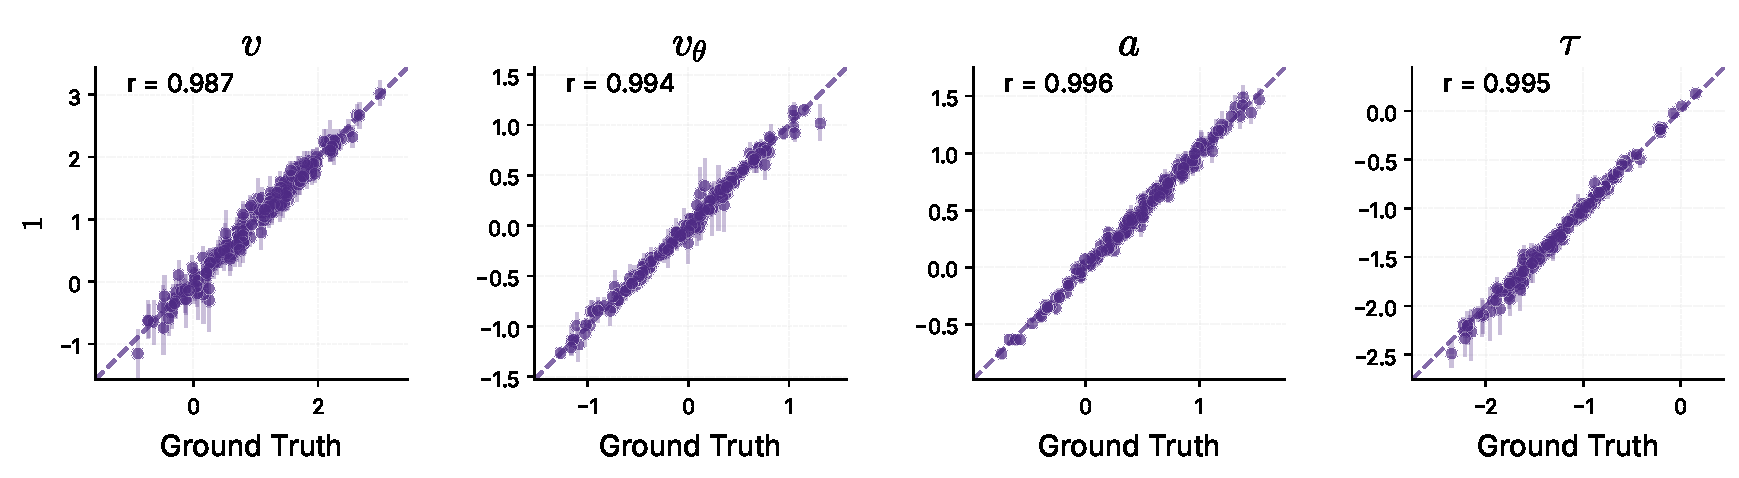
\includegraphics[width=\textwidth,height=0.3\textheight,keepaspectratio]{cdm/fixed/cf_recovery.pdf}\par\vspace{1ex}
  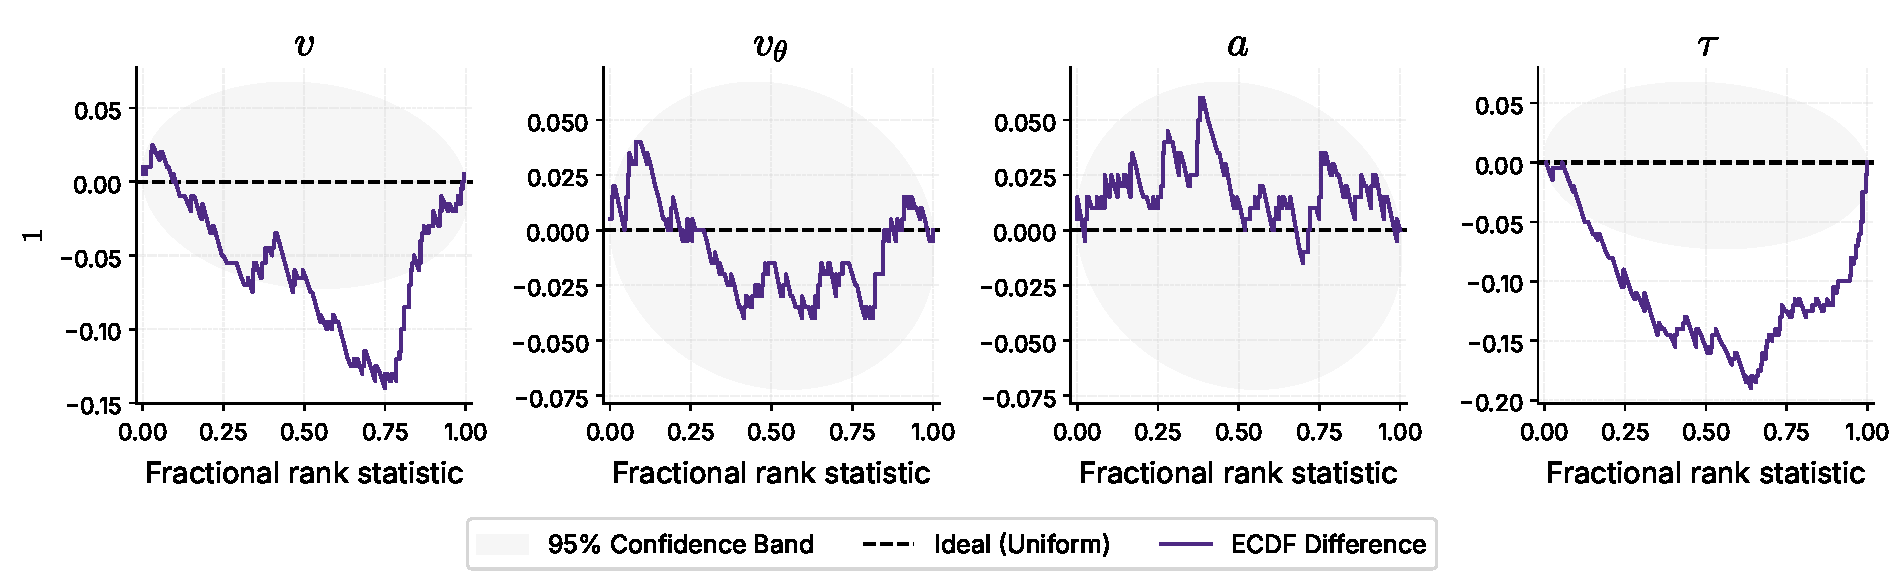
\includegraphics[width=\textwidth,height=0.3\textheight,keepaspectratio]{cdm/fixed/cf_ecdf.pdf}\par\vspace{1ex}
  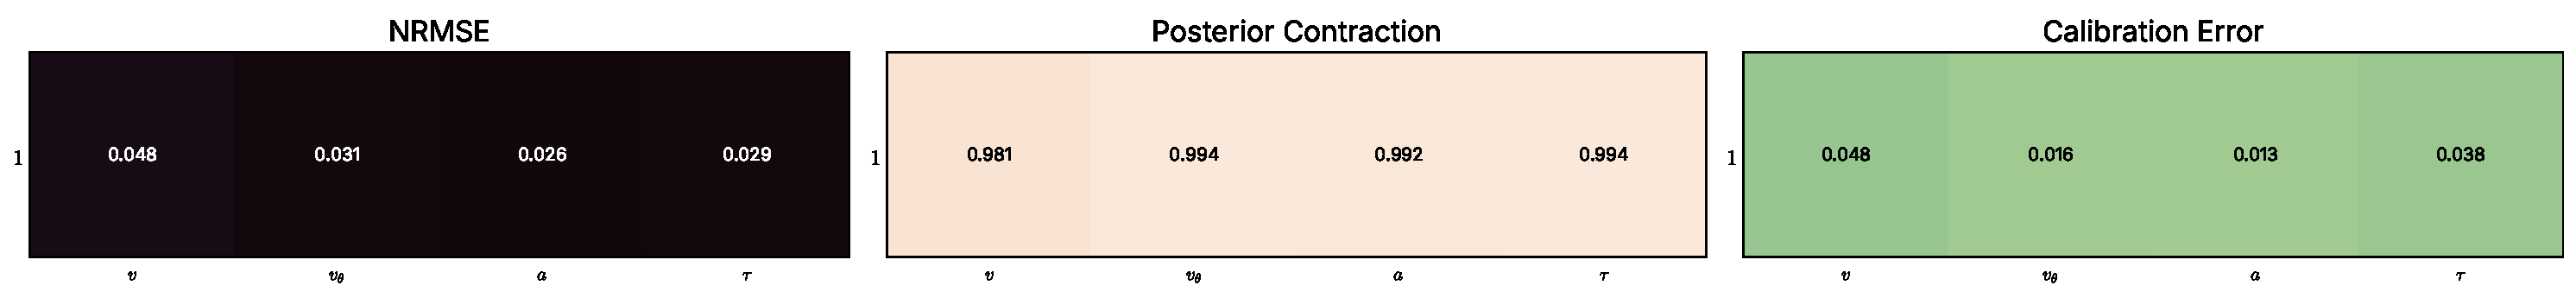
\includegraphics[width=\textwidth]{cdm/fixed/cf_metrics.pdf}
  \caption{\textbf{CDM, \emph{fixed} design: CogFormer.} Recovery (top), calibration (middle), metrics (bottom). $s_v$ and $s_\tau$ are fixed at 0 and not estimated; every estimated parameter enters as an intercept only (4 coefficients shown). Layout and encoding as in Figure~\ref{fig:app1-ddm-intercept-only-cf}.}
  \label{fig:app1-cdm-fixed-cf}
\end{figure}

\begin{figure}[p]
  \centering
  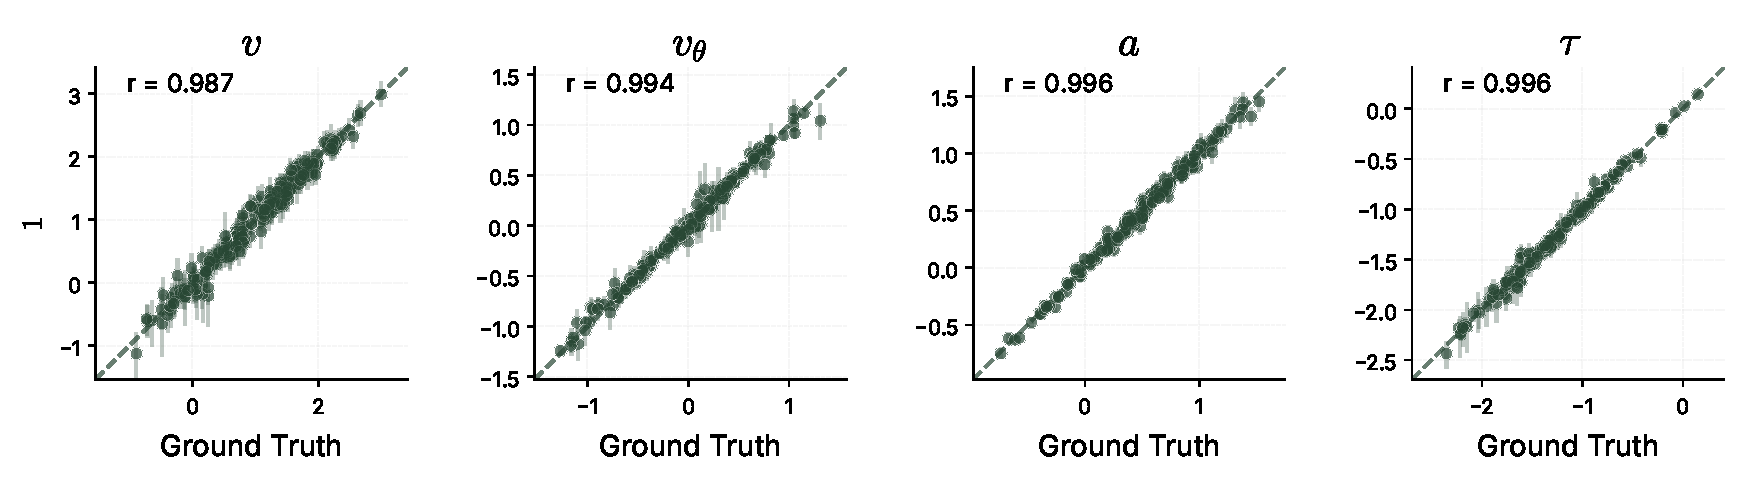
\includegraphics[width=\textwidth,height=0.3\textheight,keepaspectratio]{cdm/fixed/bf_recovery.pdf}\par\vspace{1ex}
  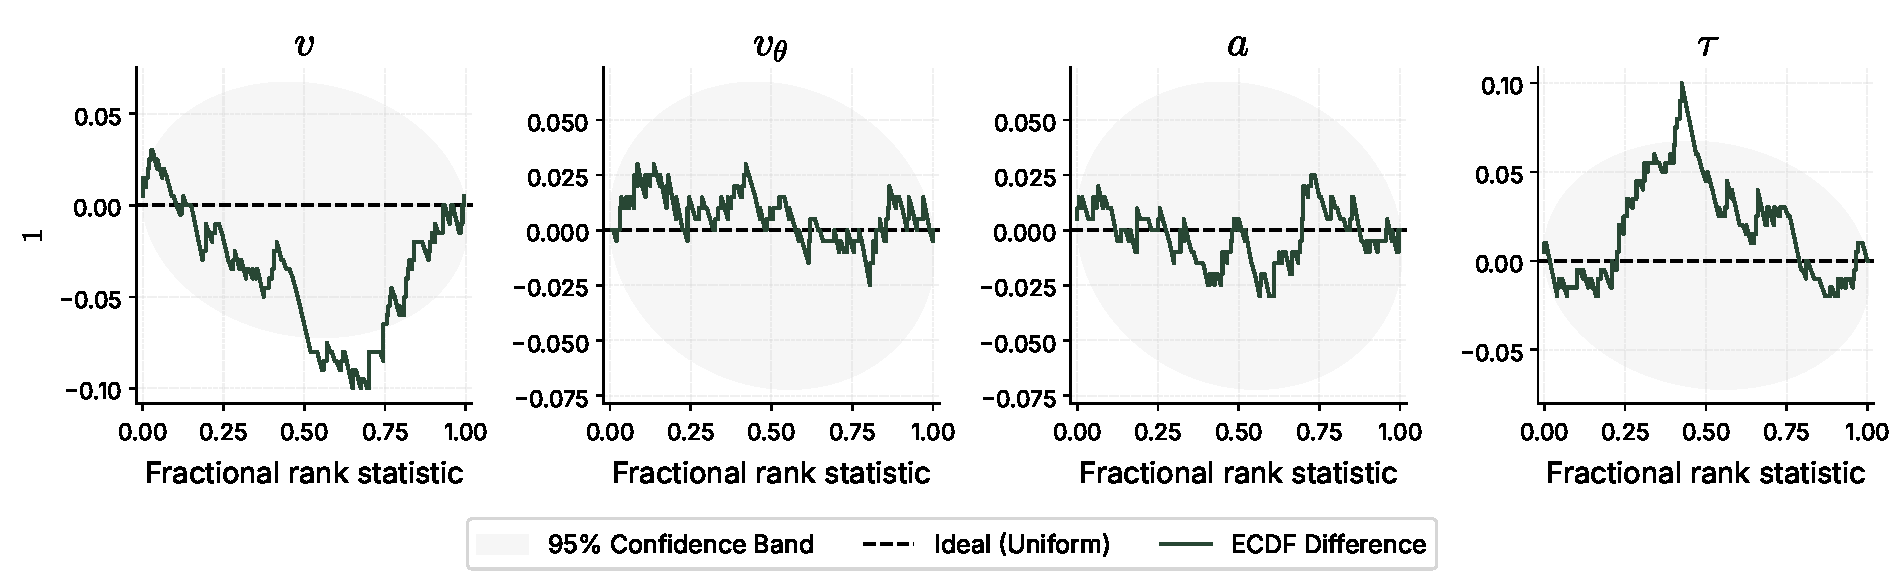
\includegraphics[width=\textwidth,height=0.3\textheight,keepaspectratio]{cdm/fixed/bf_ecdf.pdf}\par\vspace{1ex}
  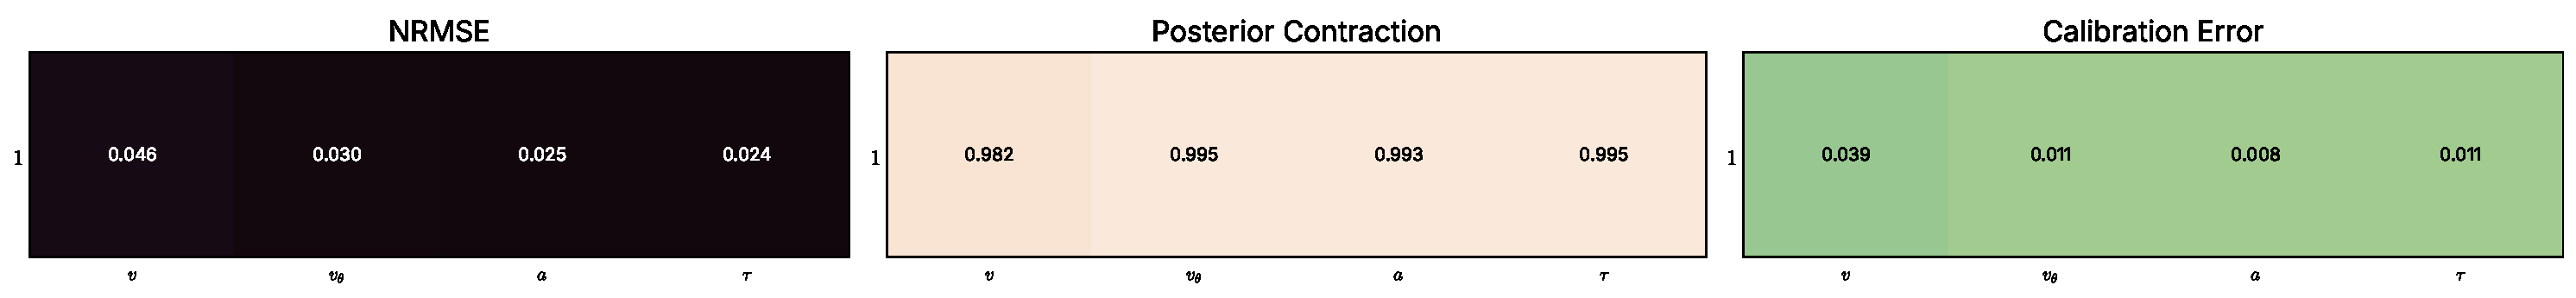
\includegraphics[width=\textwidth]{cdm/fixed/bf_metrics.pdf}
  \caption{\textbf{CDM, \emph{fixed} design: BayesFlow baseline.} Recovery (top), calibration (middle), metrics (bottom). $s_v$ and $s_\tau$ are fixed at 0 and not estimated; every estimated parameter enters as an intercept only (4 coefficients shown). Layout and encoding as in Figure~\ref{fig:app1-ddm-intercept-only-cf}.}
  \label{fig:app1-cdm-fixed-bf}
\end{figure}

\begin{figure}[p]
  \centering
  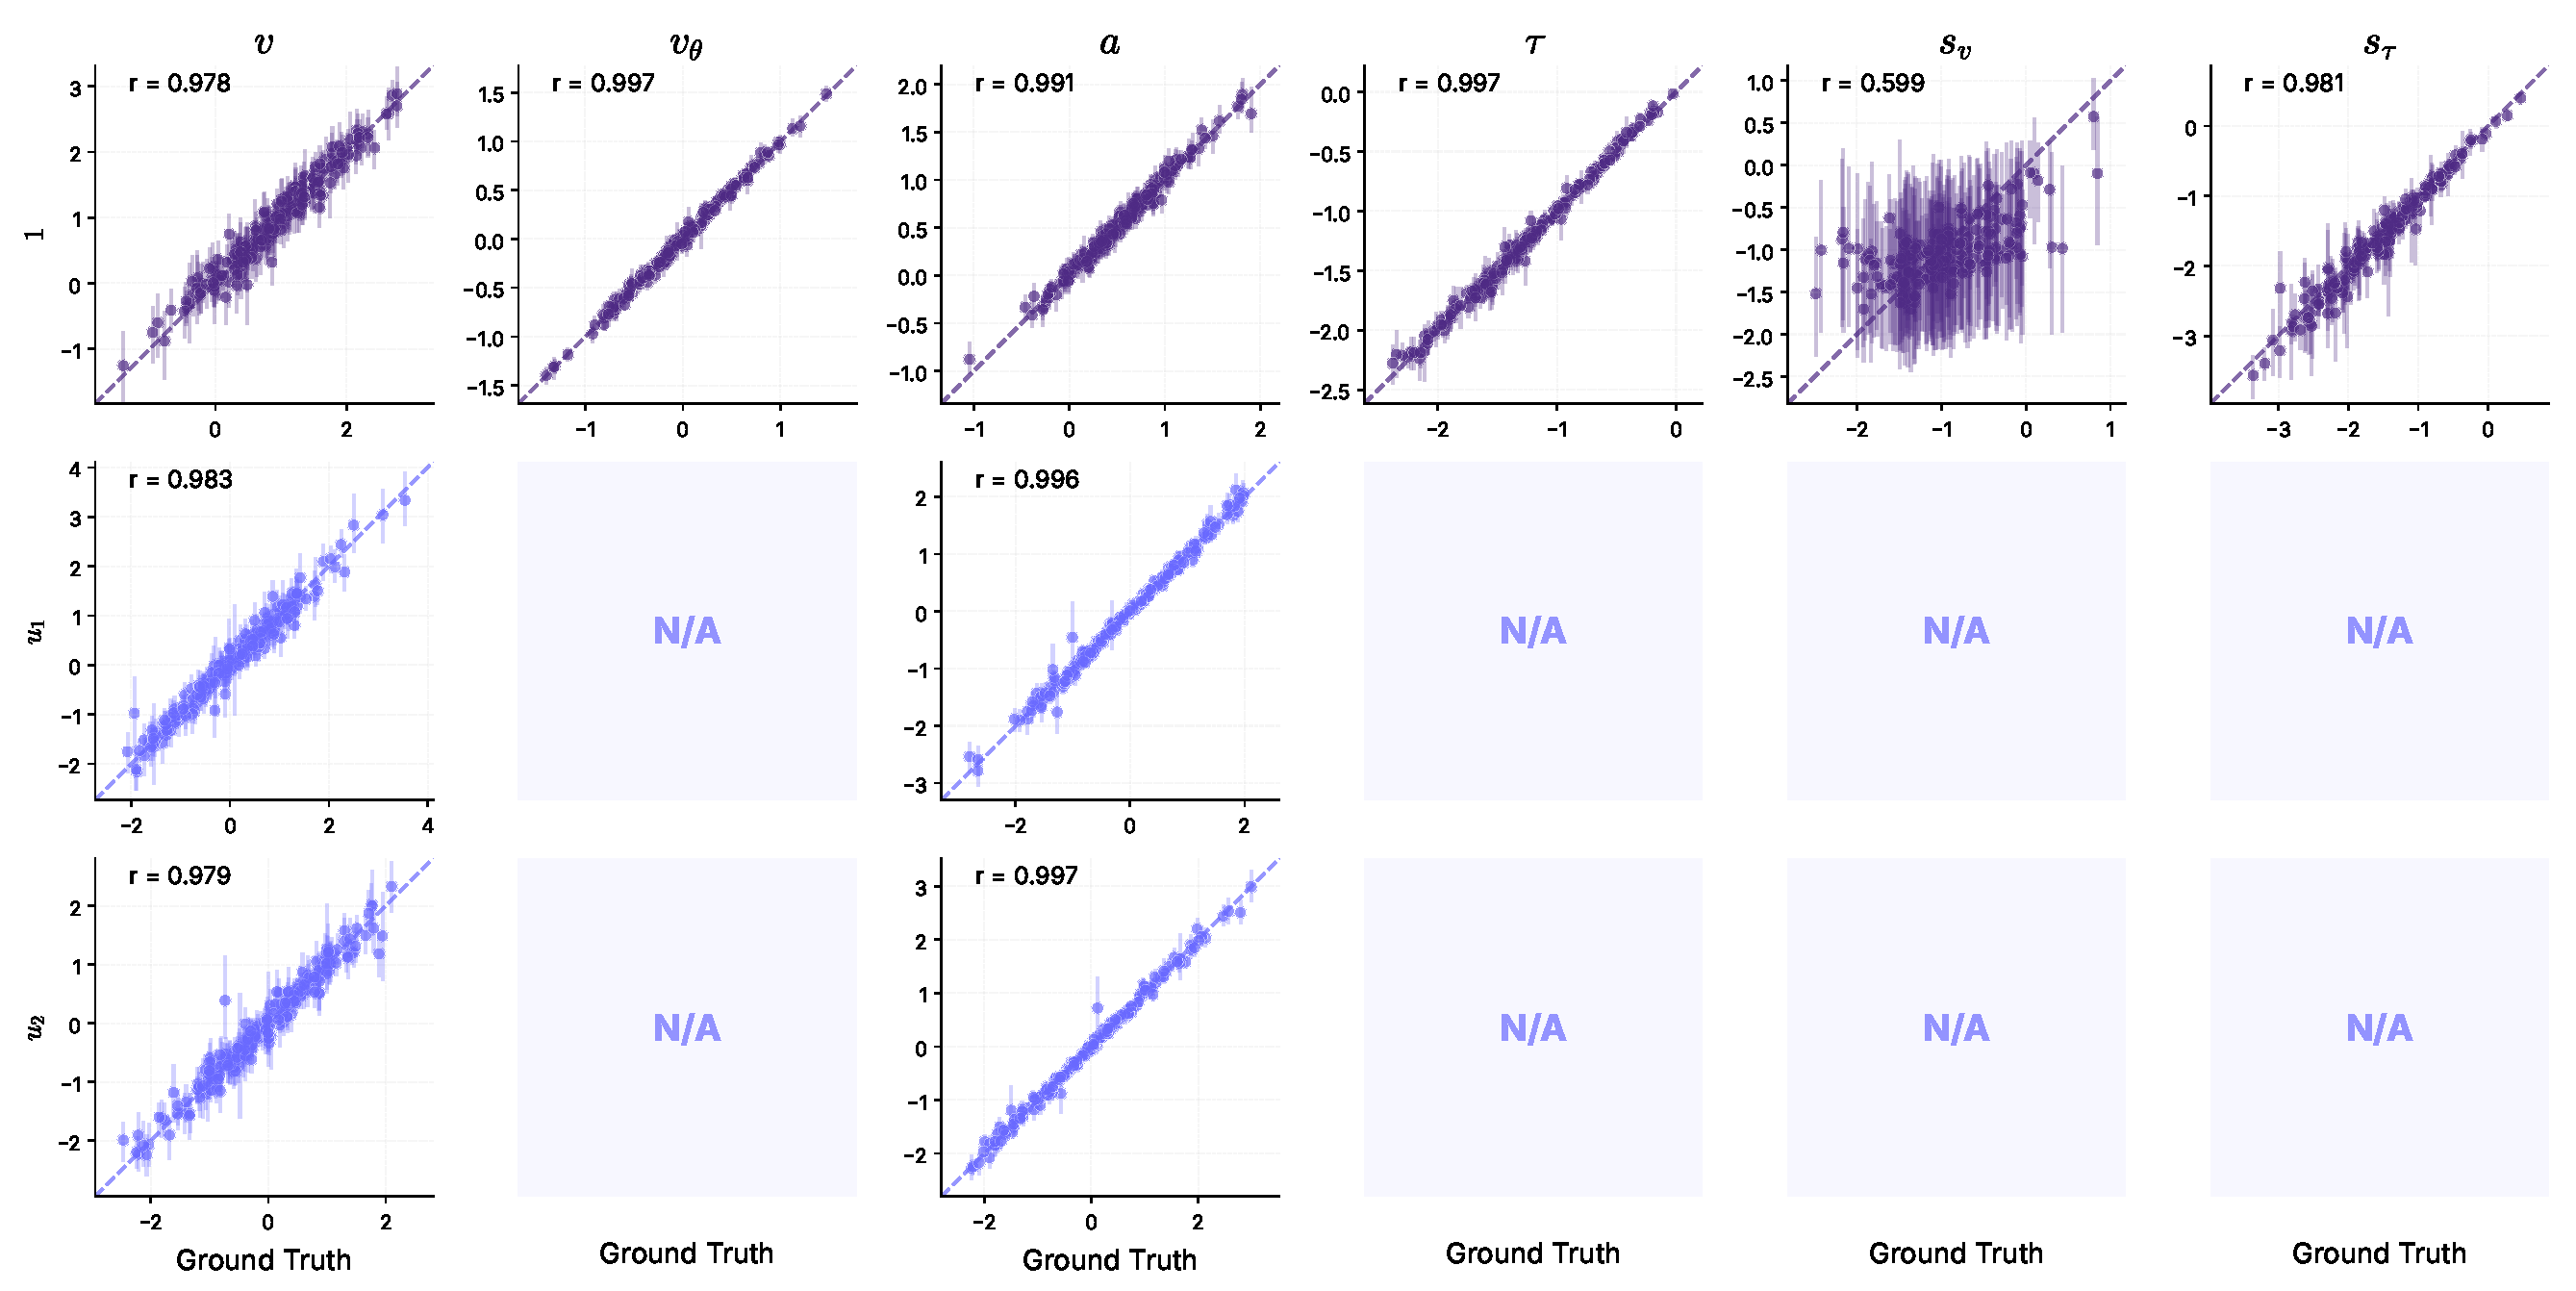
\includegraphics[width=\textwidth,height=0.3\textheight,keepaspectratio]{cdm/regressed/cf_recovery.pdf}\par\vspace{1ex}
  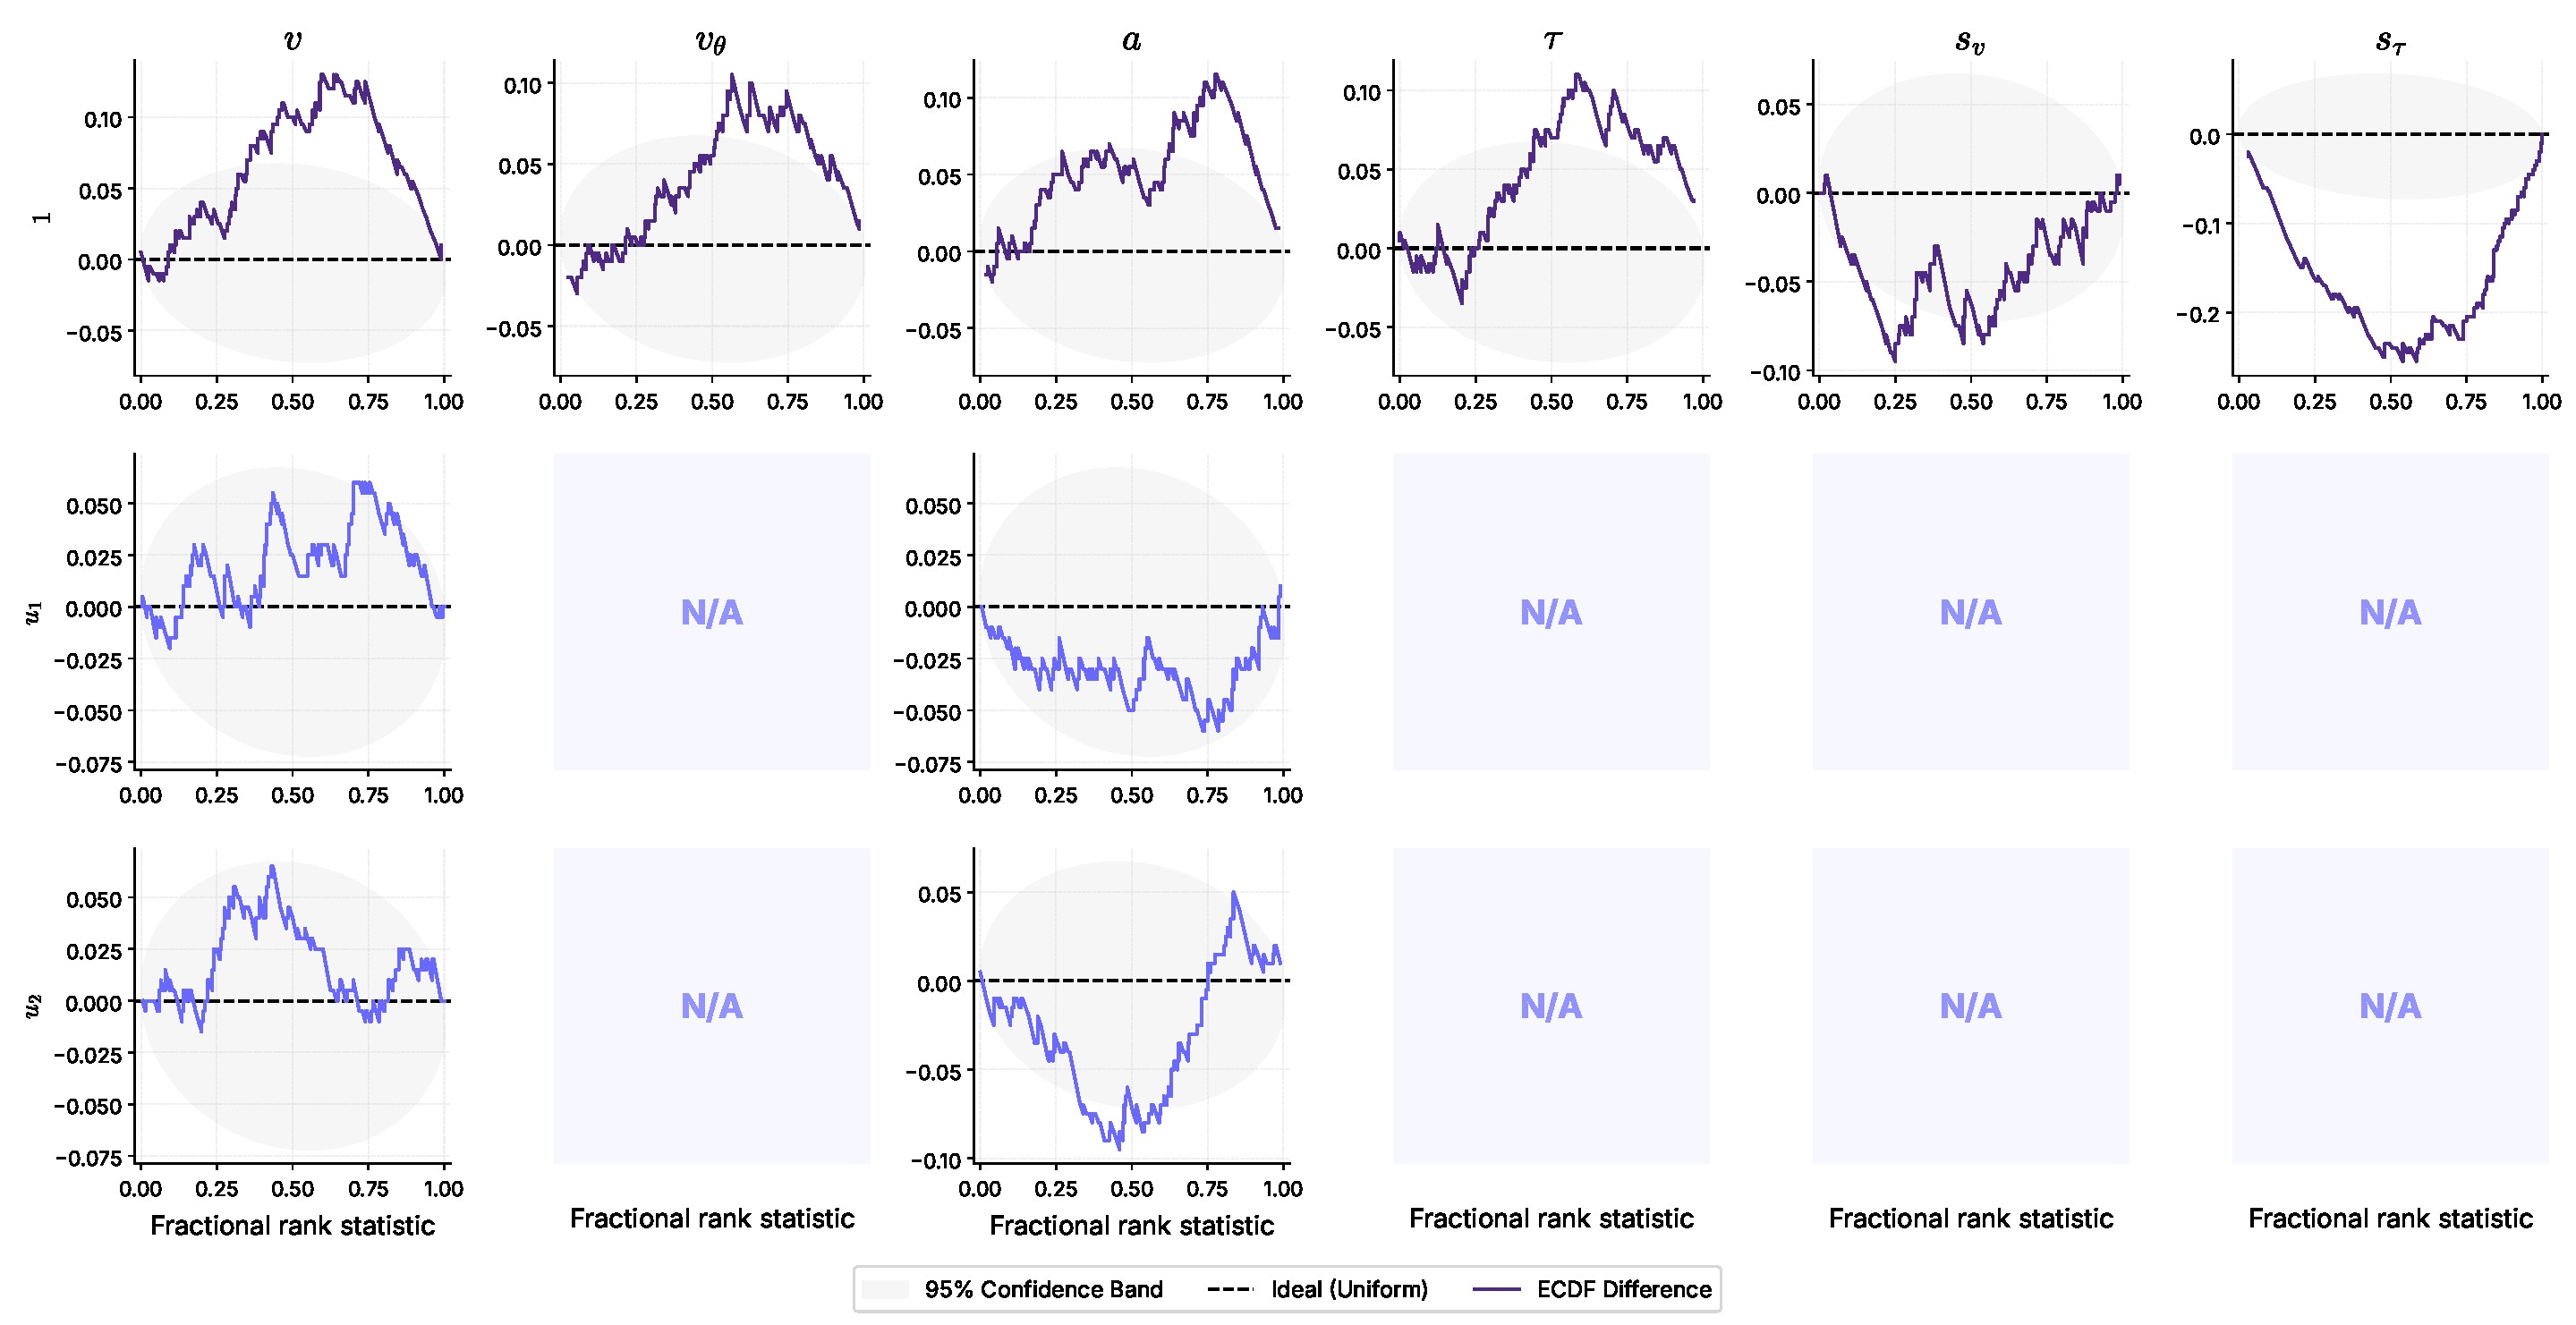
\includegraphics[width=\textwidth,height=0.3\textheight,keepaspectratio]{cdm/regressed/cf_ecdf.pdf}\par\vspace{1ex}
  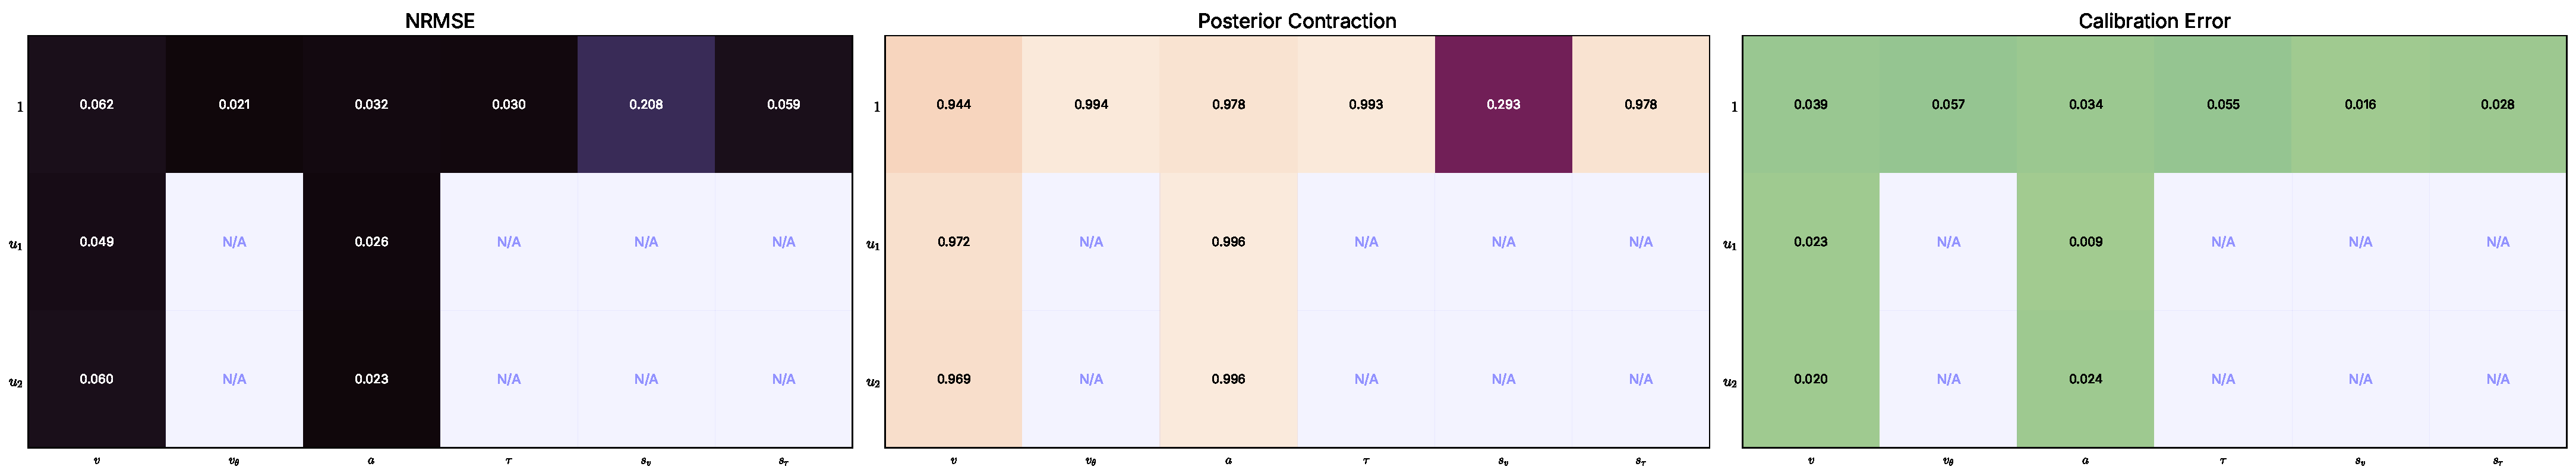
\includegraphics[width=\textwidth]{cdm/regressed/cf_metrics.pdf}
  \caption{\textbf{CDM, \emph{regressed} design: CogFormer.} Recovery (top), calibration (middle), metrics (bottom). $v$ and $a$ carry slopes on $u_1$ and $u_2$ (10 coefficients shown). Layout and encoding as in Figure~\ref{fig:app1-ddm-intercept-only-cf}.}
  \label{fig:app1-cdm-regressed-cf}
\end{figure}

\begin{figure}[p]
  \centering
  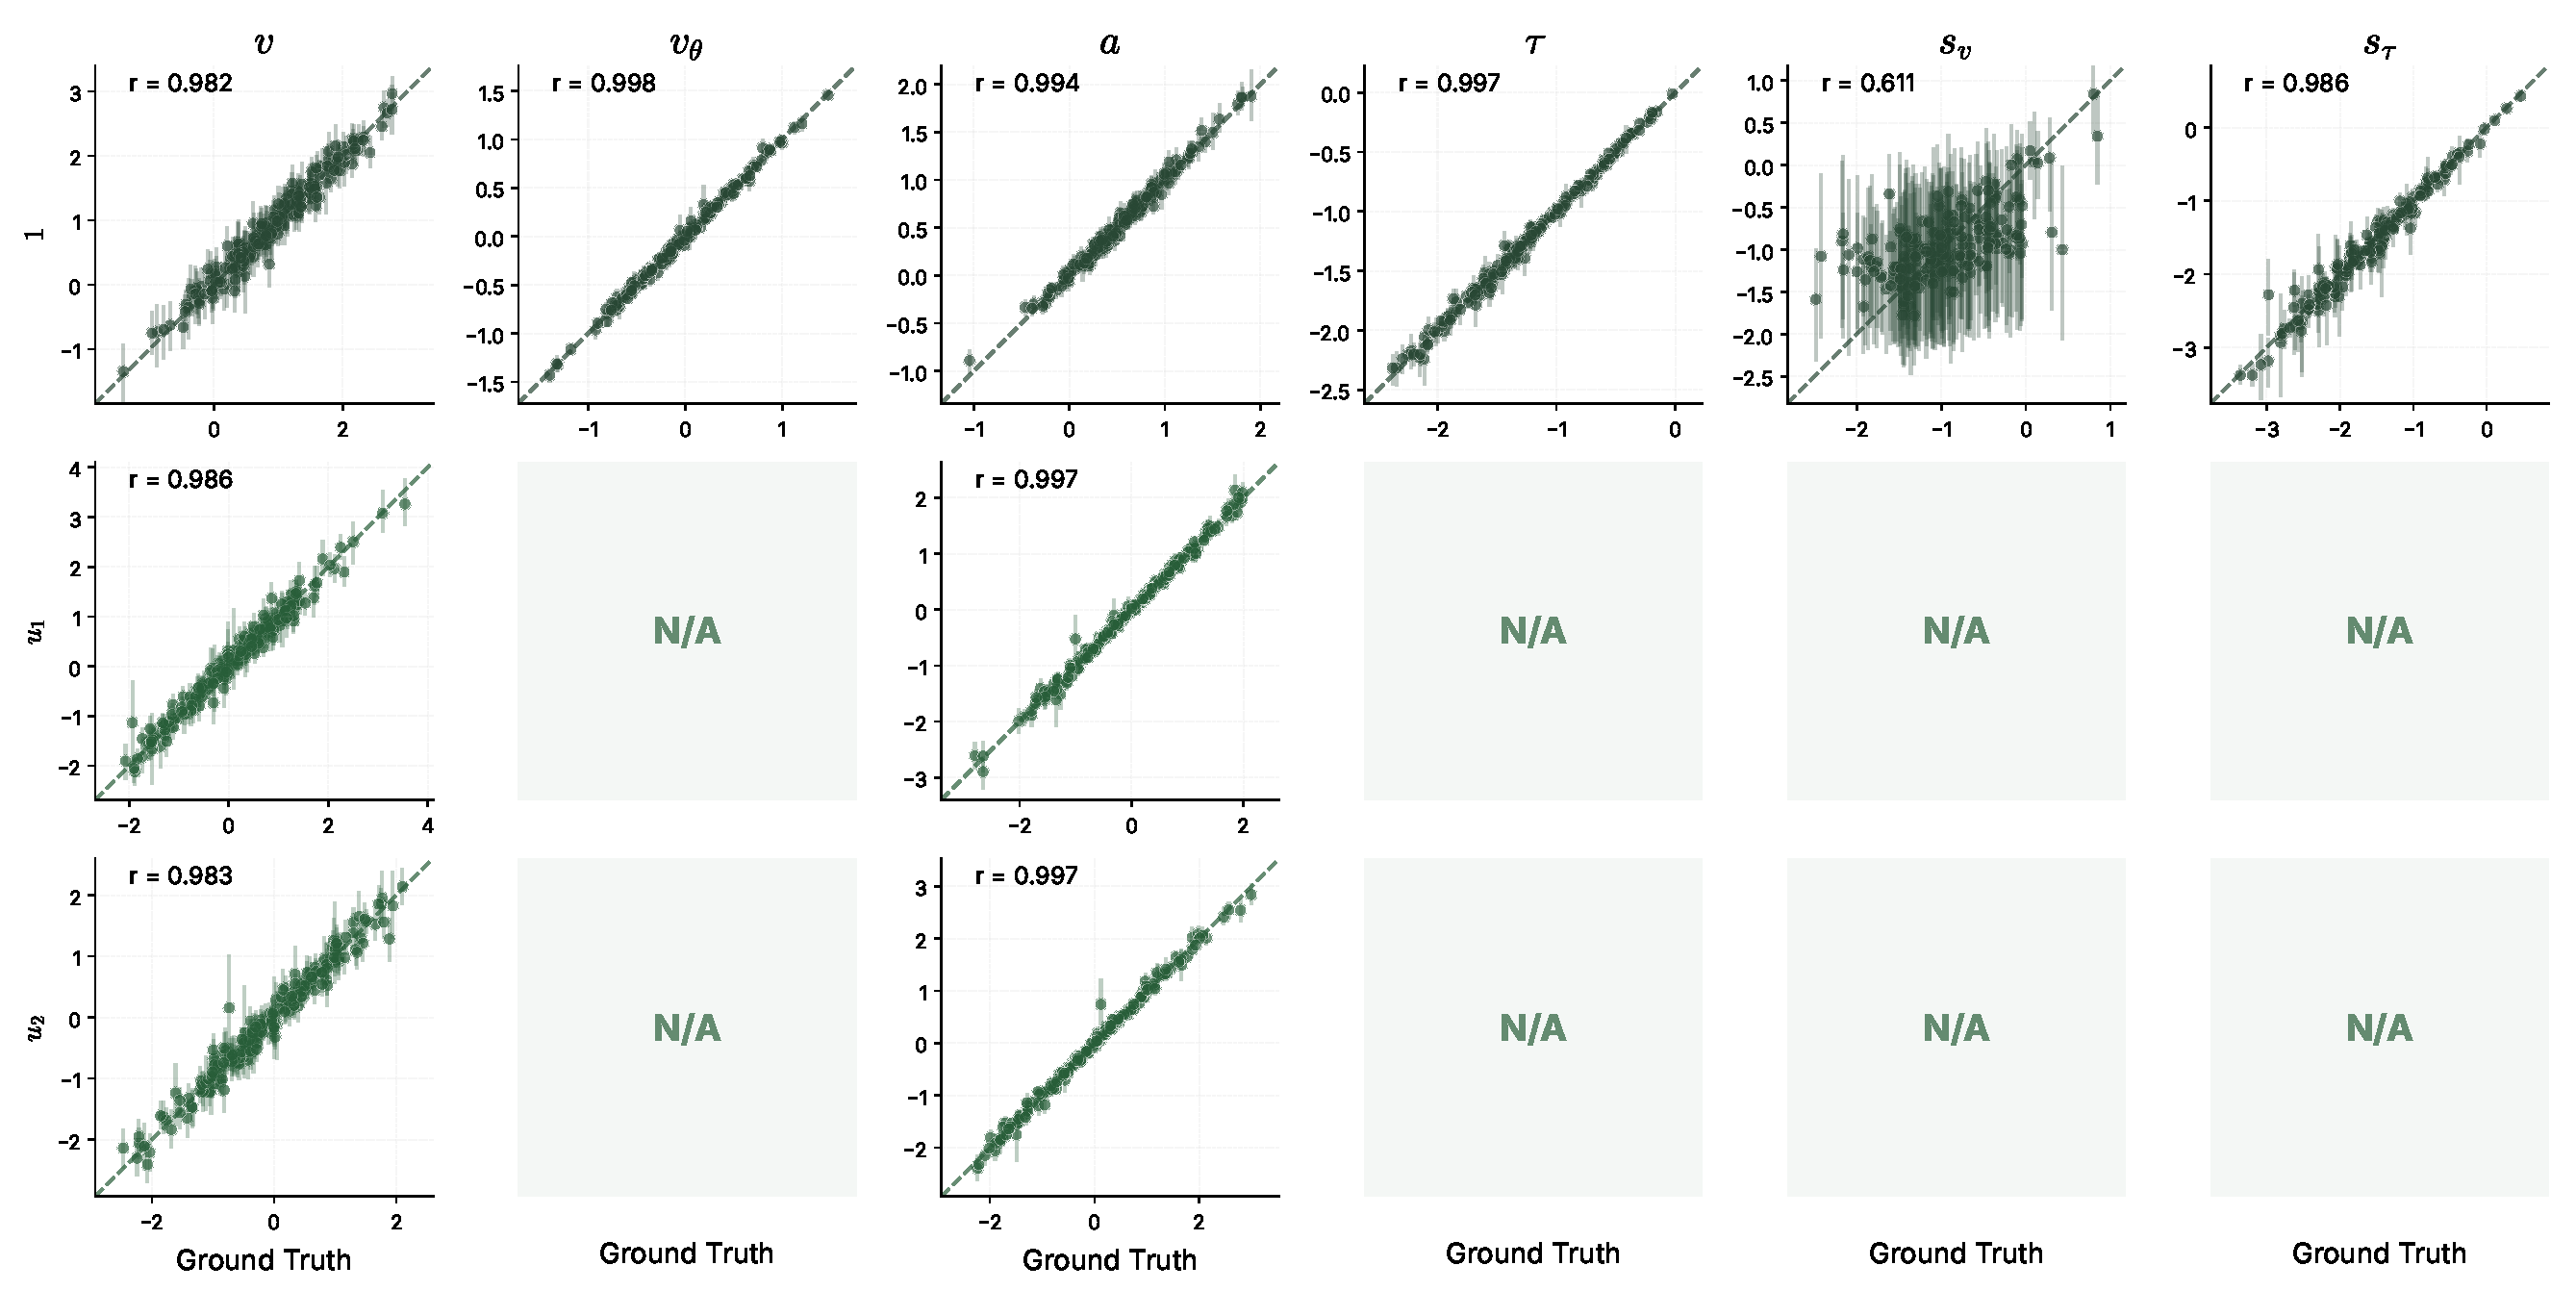
\includegraphics[width=\textwidth,height=0.3\textheight,keepaspectratio]{cdm/regressed/bf_recovery.pdf}\par\vspace{1ex}
  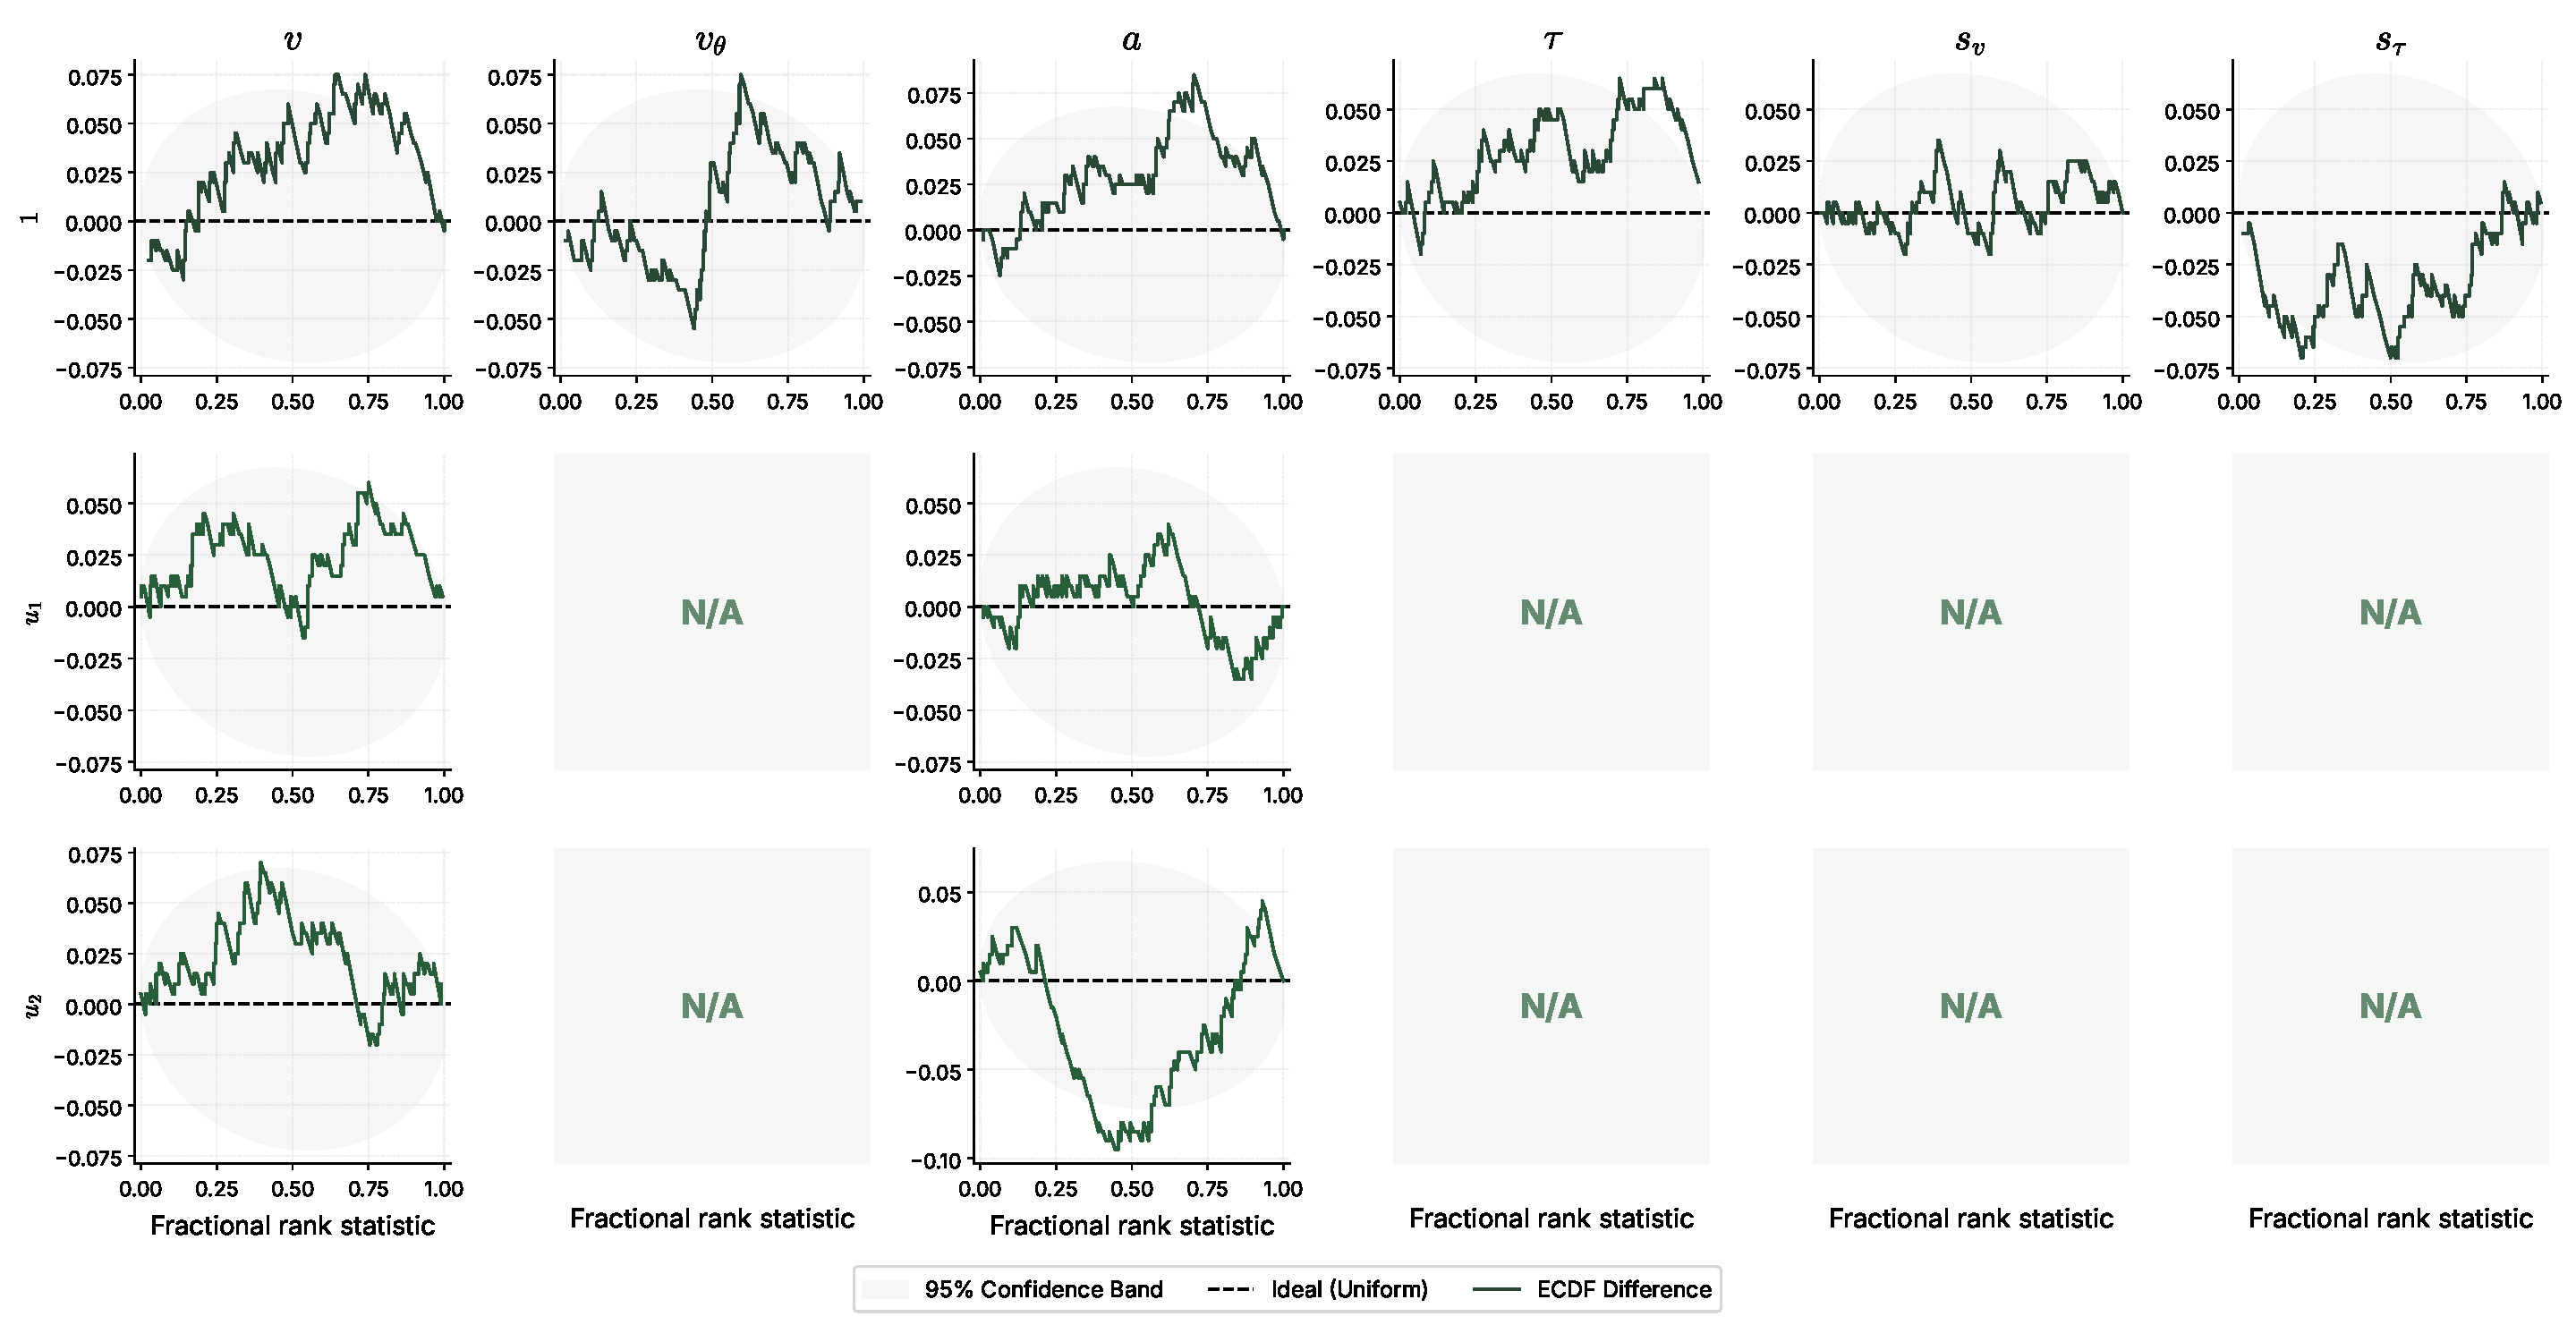
\includegraphics[width=\textwidth,height=0.3\textheight,keepaspectratio]{cdm/regressed/bf_ecdf.pdf}\par\vspace{1ex}
  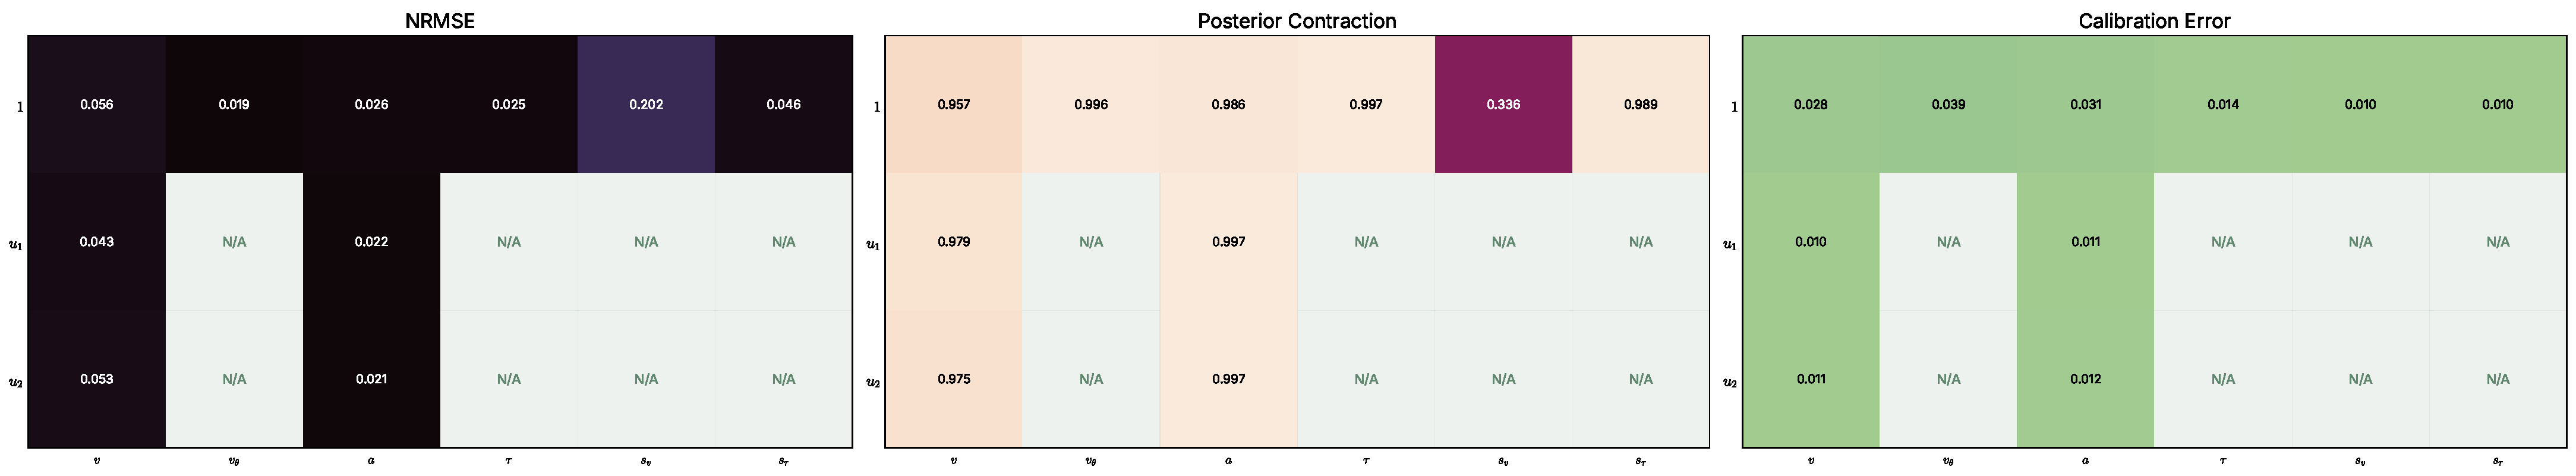
\includegraphics[width=\textwidth]{cdm/regressed/bf_metrics.pdf}
  \caption{\textbf{CDM, \emph{regressed} design: BayesFlow baseline.} Recovery (top), calibration (middle), metrics (bottom). $v$ and $a$ carry slopes on $u_1$ and $u_2$ (10 coefficients shown). Layout and encoding as in Figure~\ref{fig:app1-ddm-intercept-only-cf}.}
  \label{fig:app1-cdm-regressed-bf}
\end{figure}

\begin{figure}[p]
  \centering
  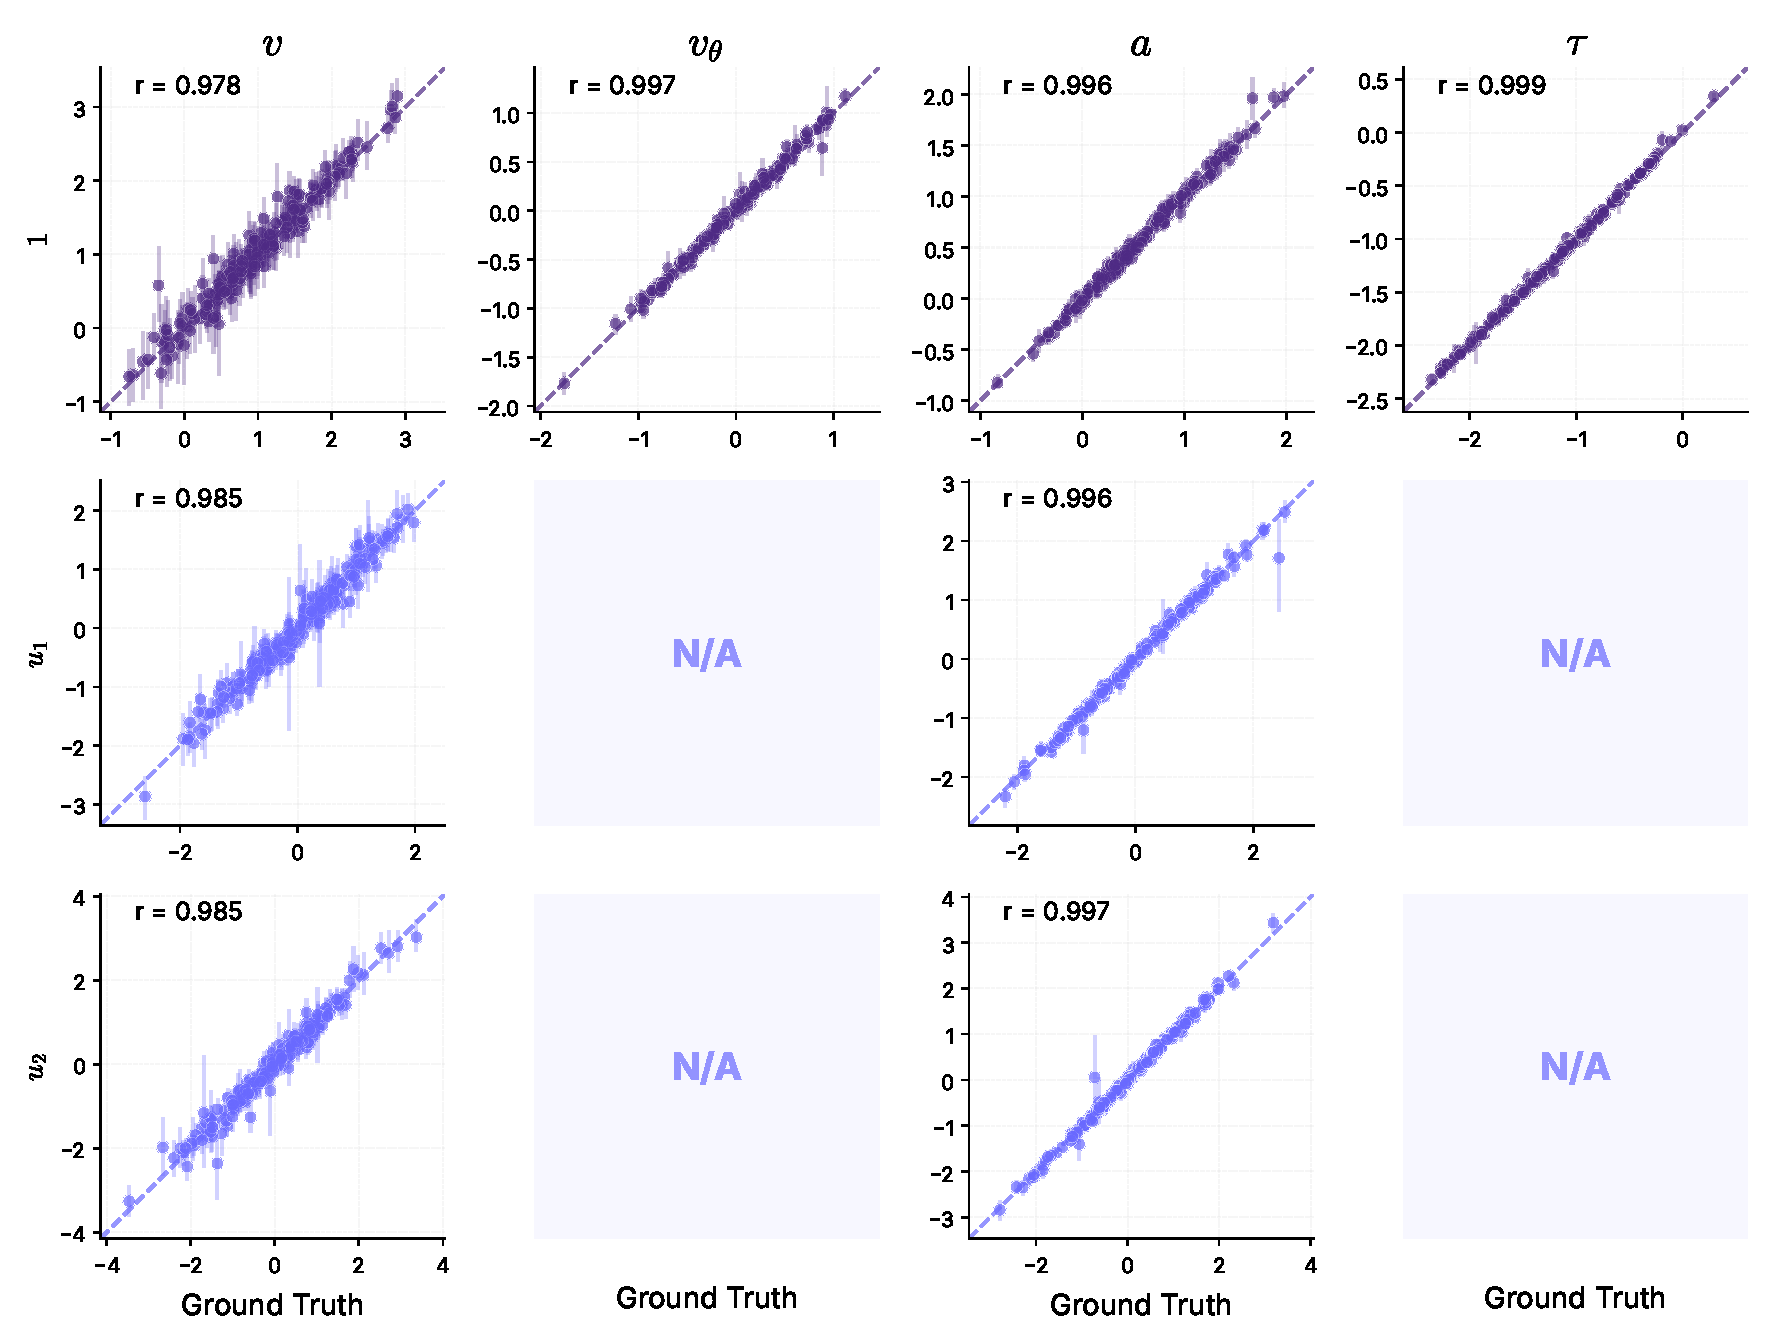
\includegraphics[width=\textwidth,height=0.3\textheight,keepaspectratio]{cdm/fixed_regressed/cf_recovery.pdf}\par\vspace{1ex}
  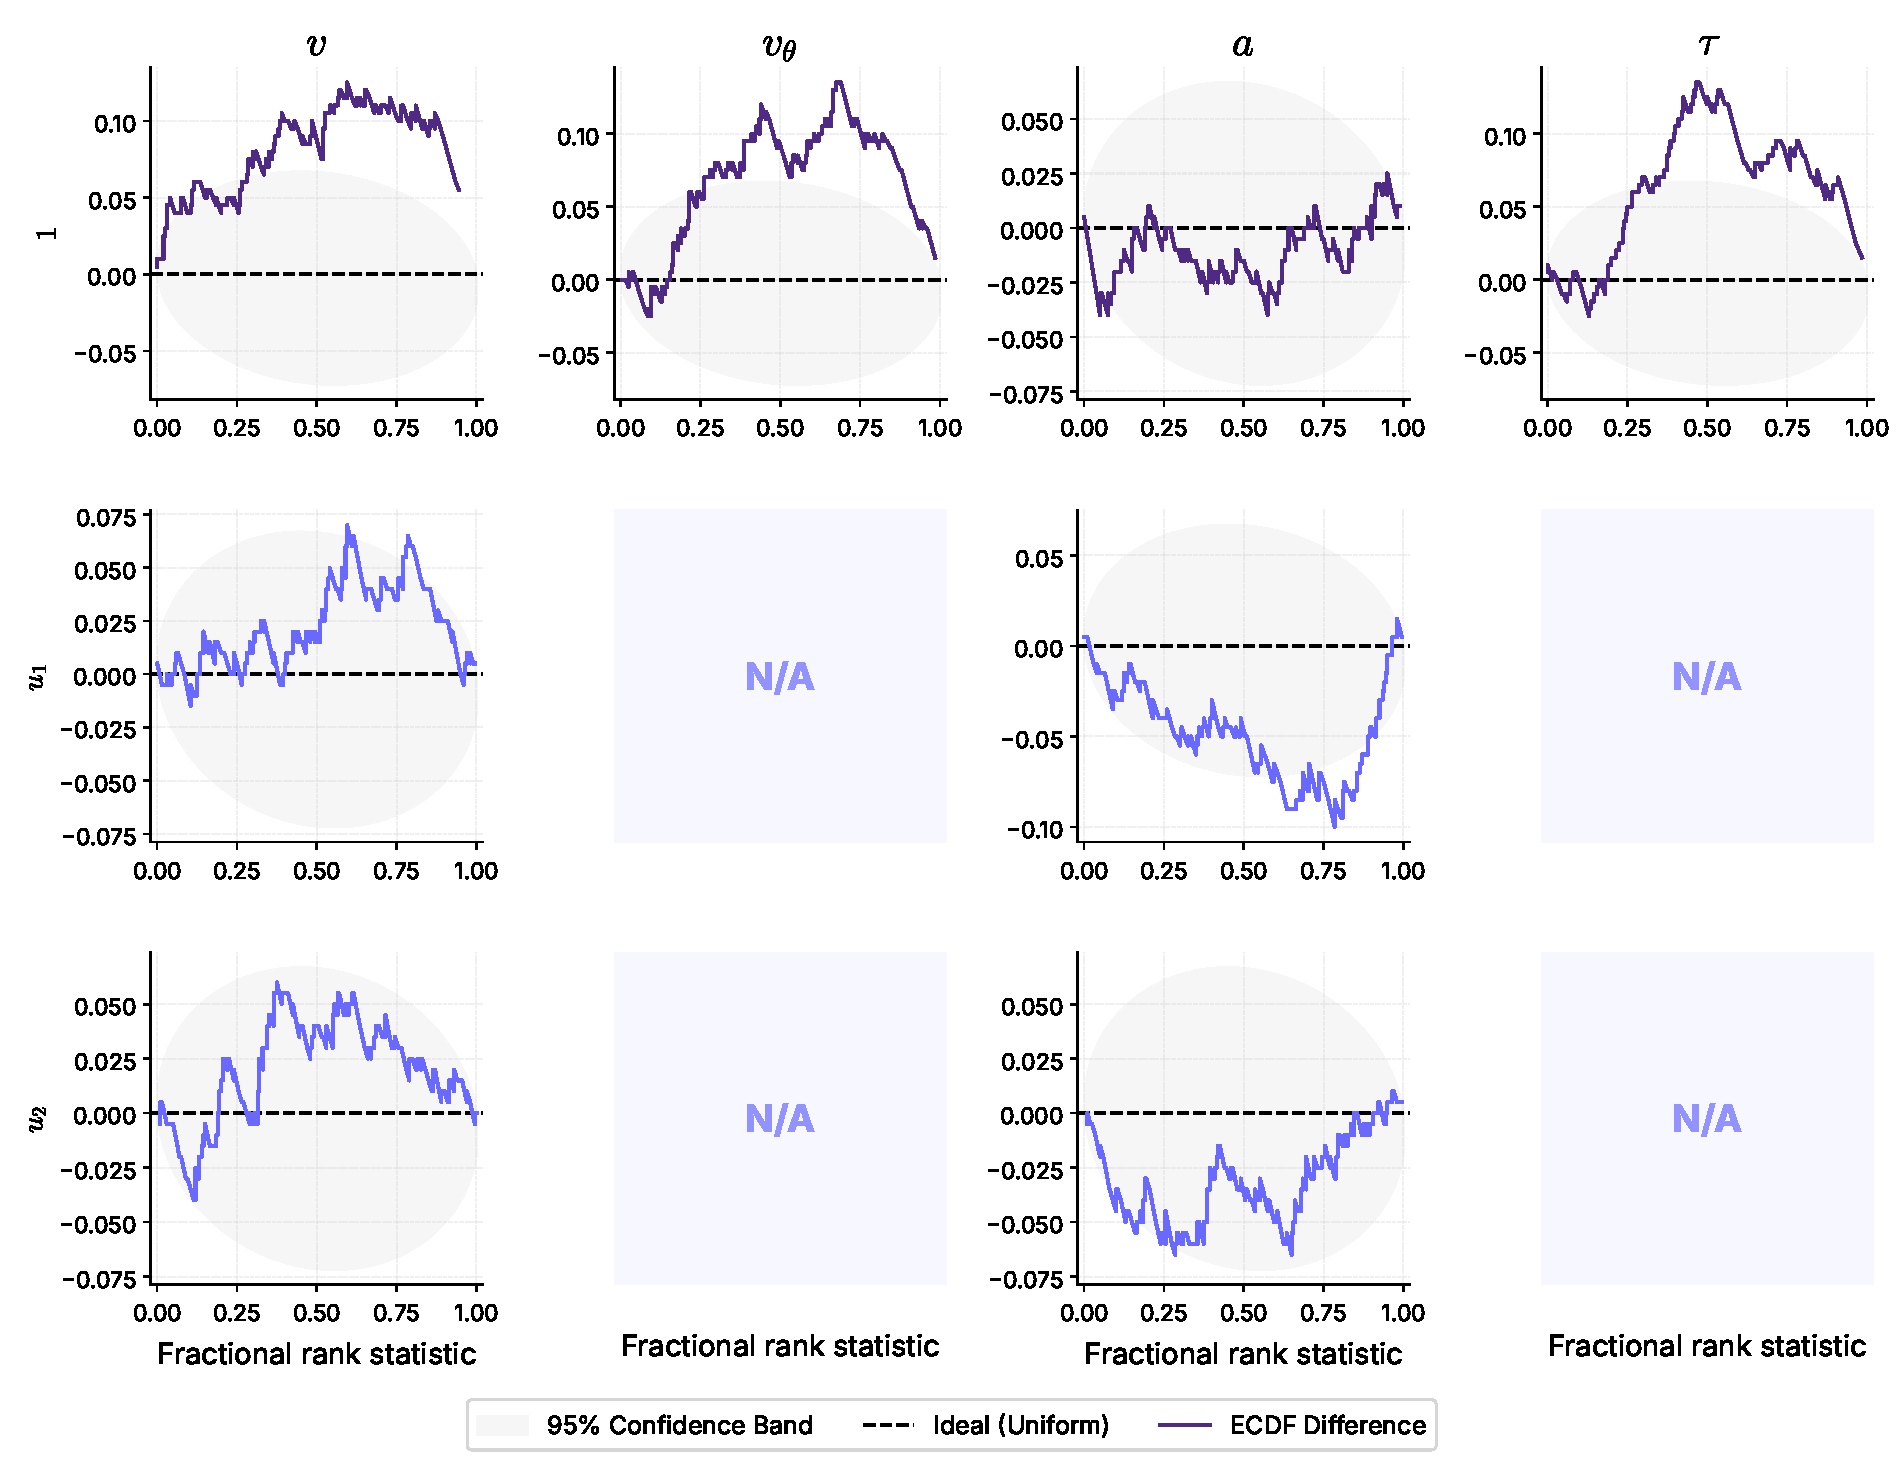
\includegraphics[width=\textwidth,height=0.3\textheight,keepaspectratio]{cdm/fixed_regressed/cf_ecdf.pdf}\par\vspace{1ex}
  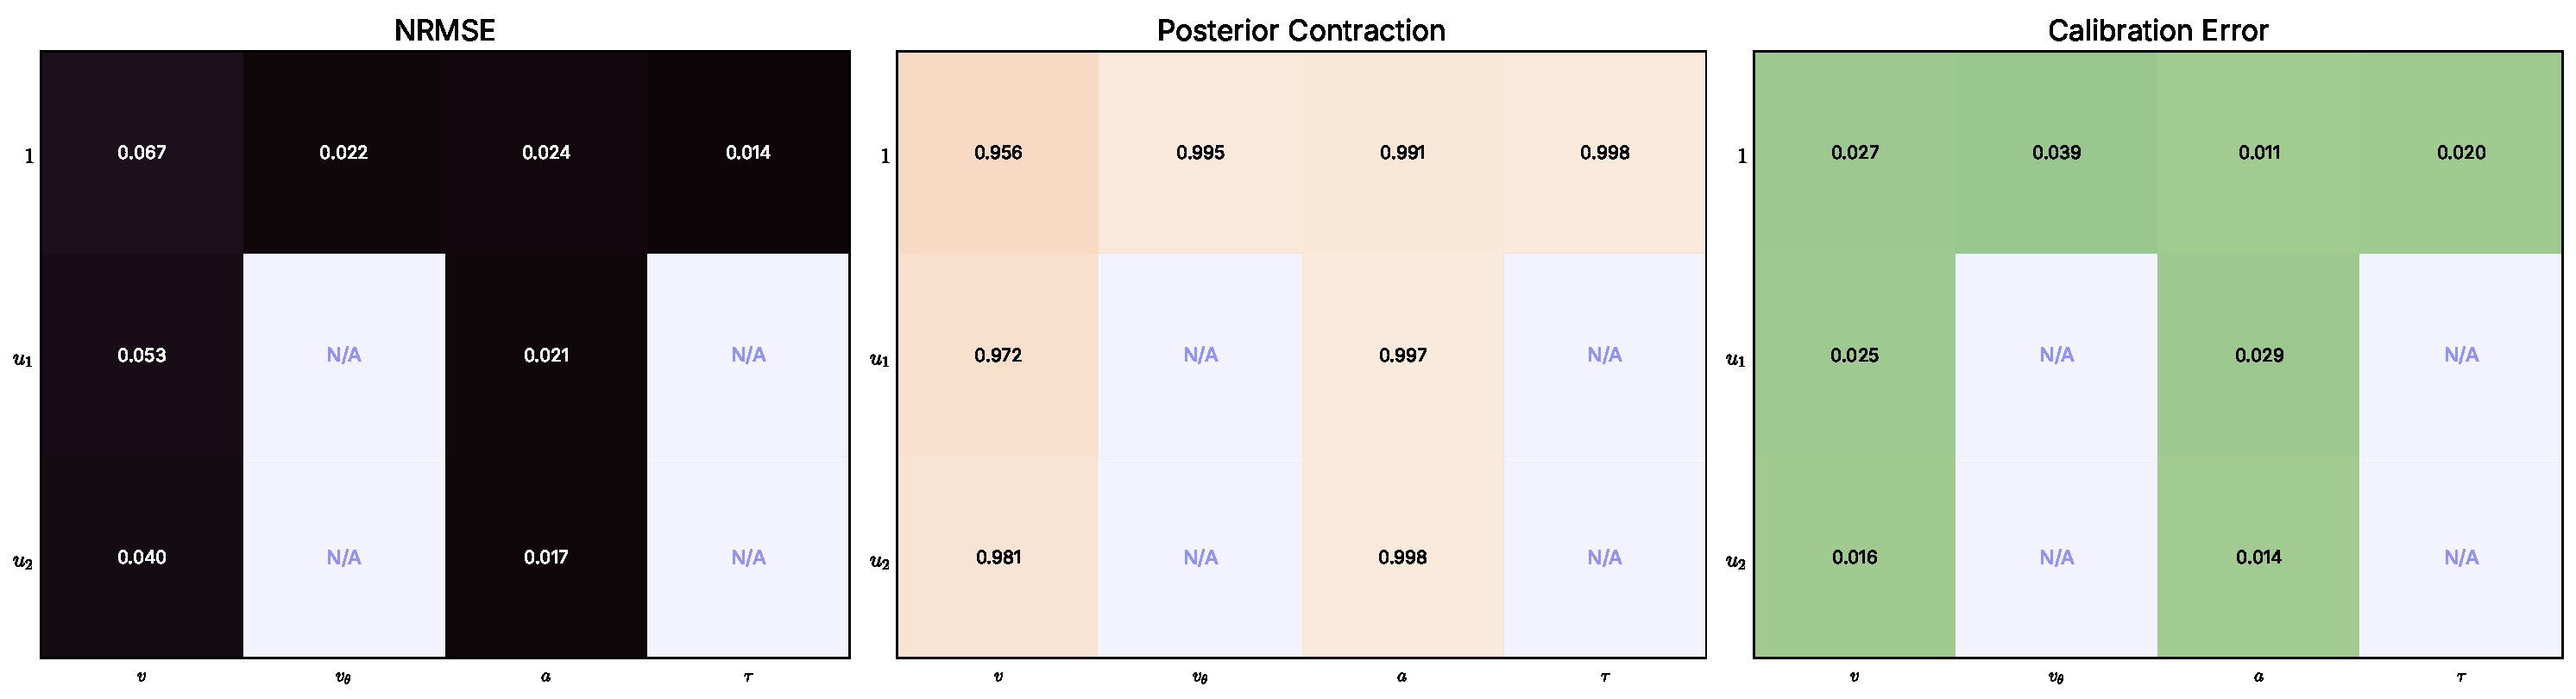
\includegraphics[width=\textwidth]{cdm/fixed_regressed/cf_metrics.pdf}
  \caption{\textbf{CDM, \emph{fixed + regressed} design: CogFormer.} Recovery (top), calibration (middle), metrics (bottom). $s_v$ and $s_\tau$ are fixed at 0 and not estimated; $v$ and $a$ carry slopes on $u_1$ and $u_2$ (8 coefficients shown). Layout and encoding as in Figure~\ref{fig:app1-ddm-intercept-only-cf}.}
  \label{fig:app1-cdm-fixed-regressed-cf}
\end{figure}

\begin{figure}[p]
  \centering
  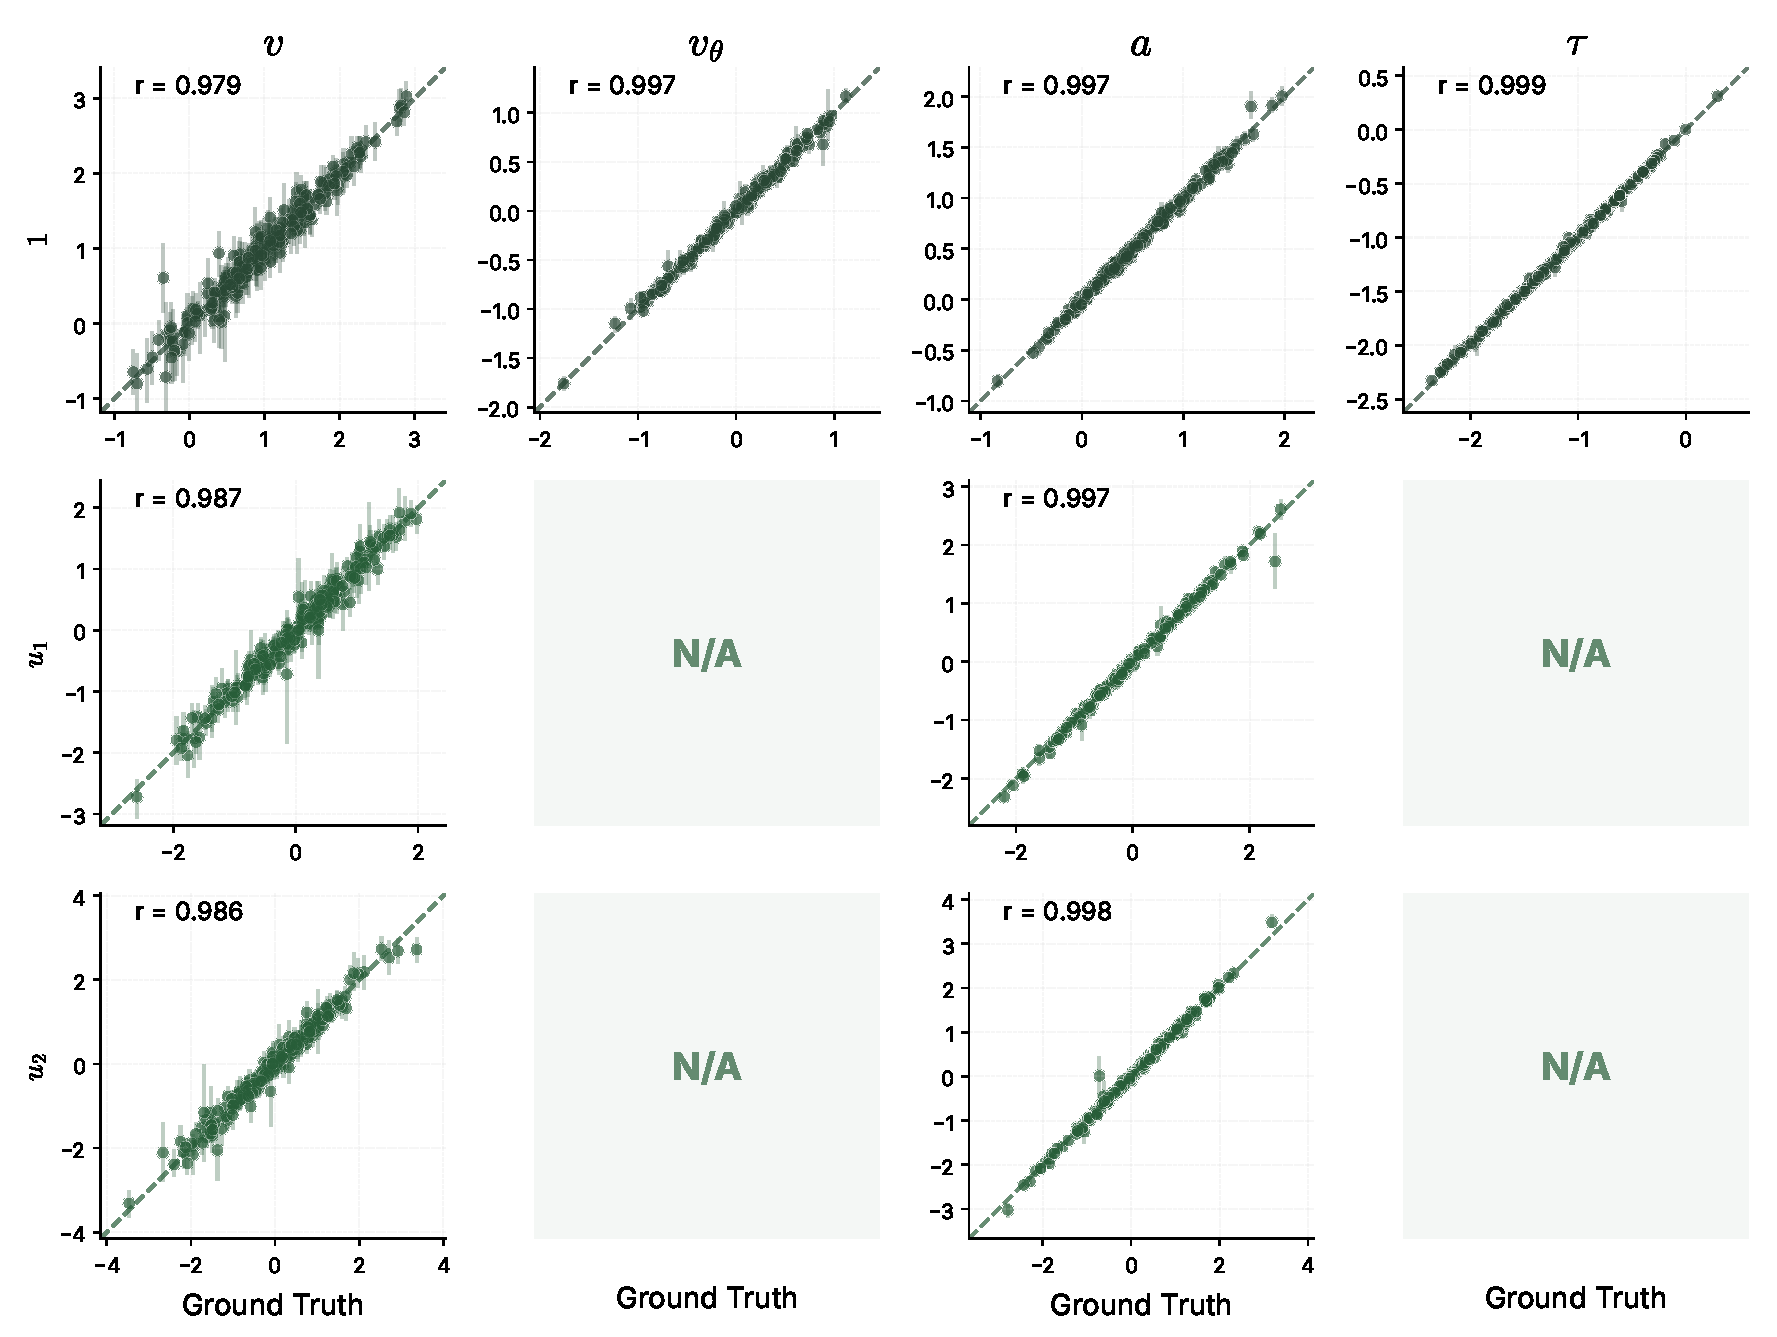
\includegraphics[width=\textwidth,height=0.3\textheight,keepaspectratio]{cdm/fixed_regressed/bf_recovery.pdf}\par\vspace{1ex}
  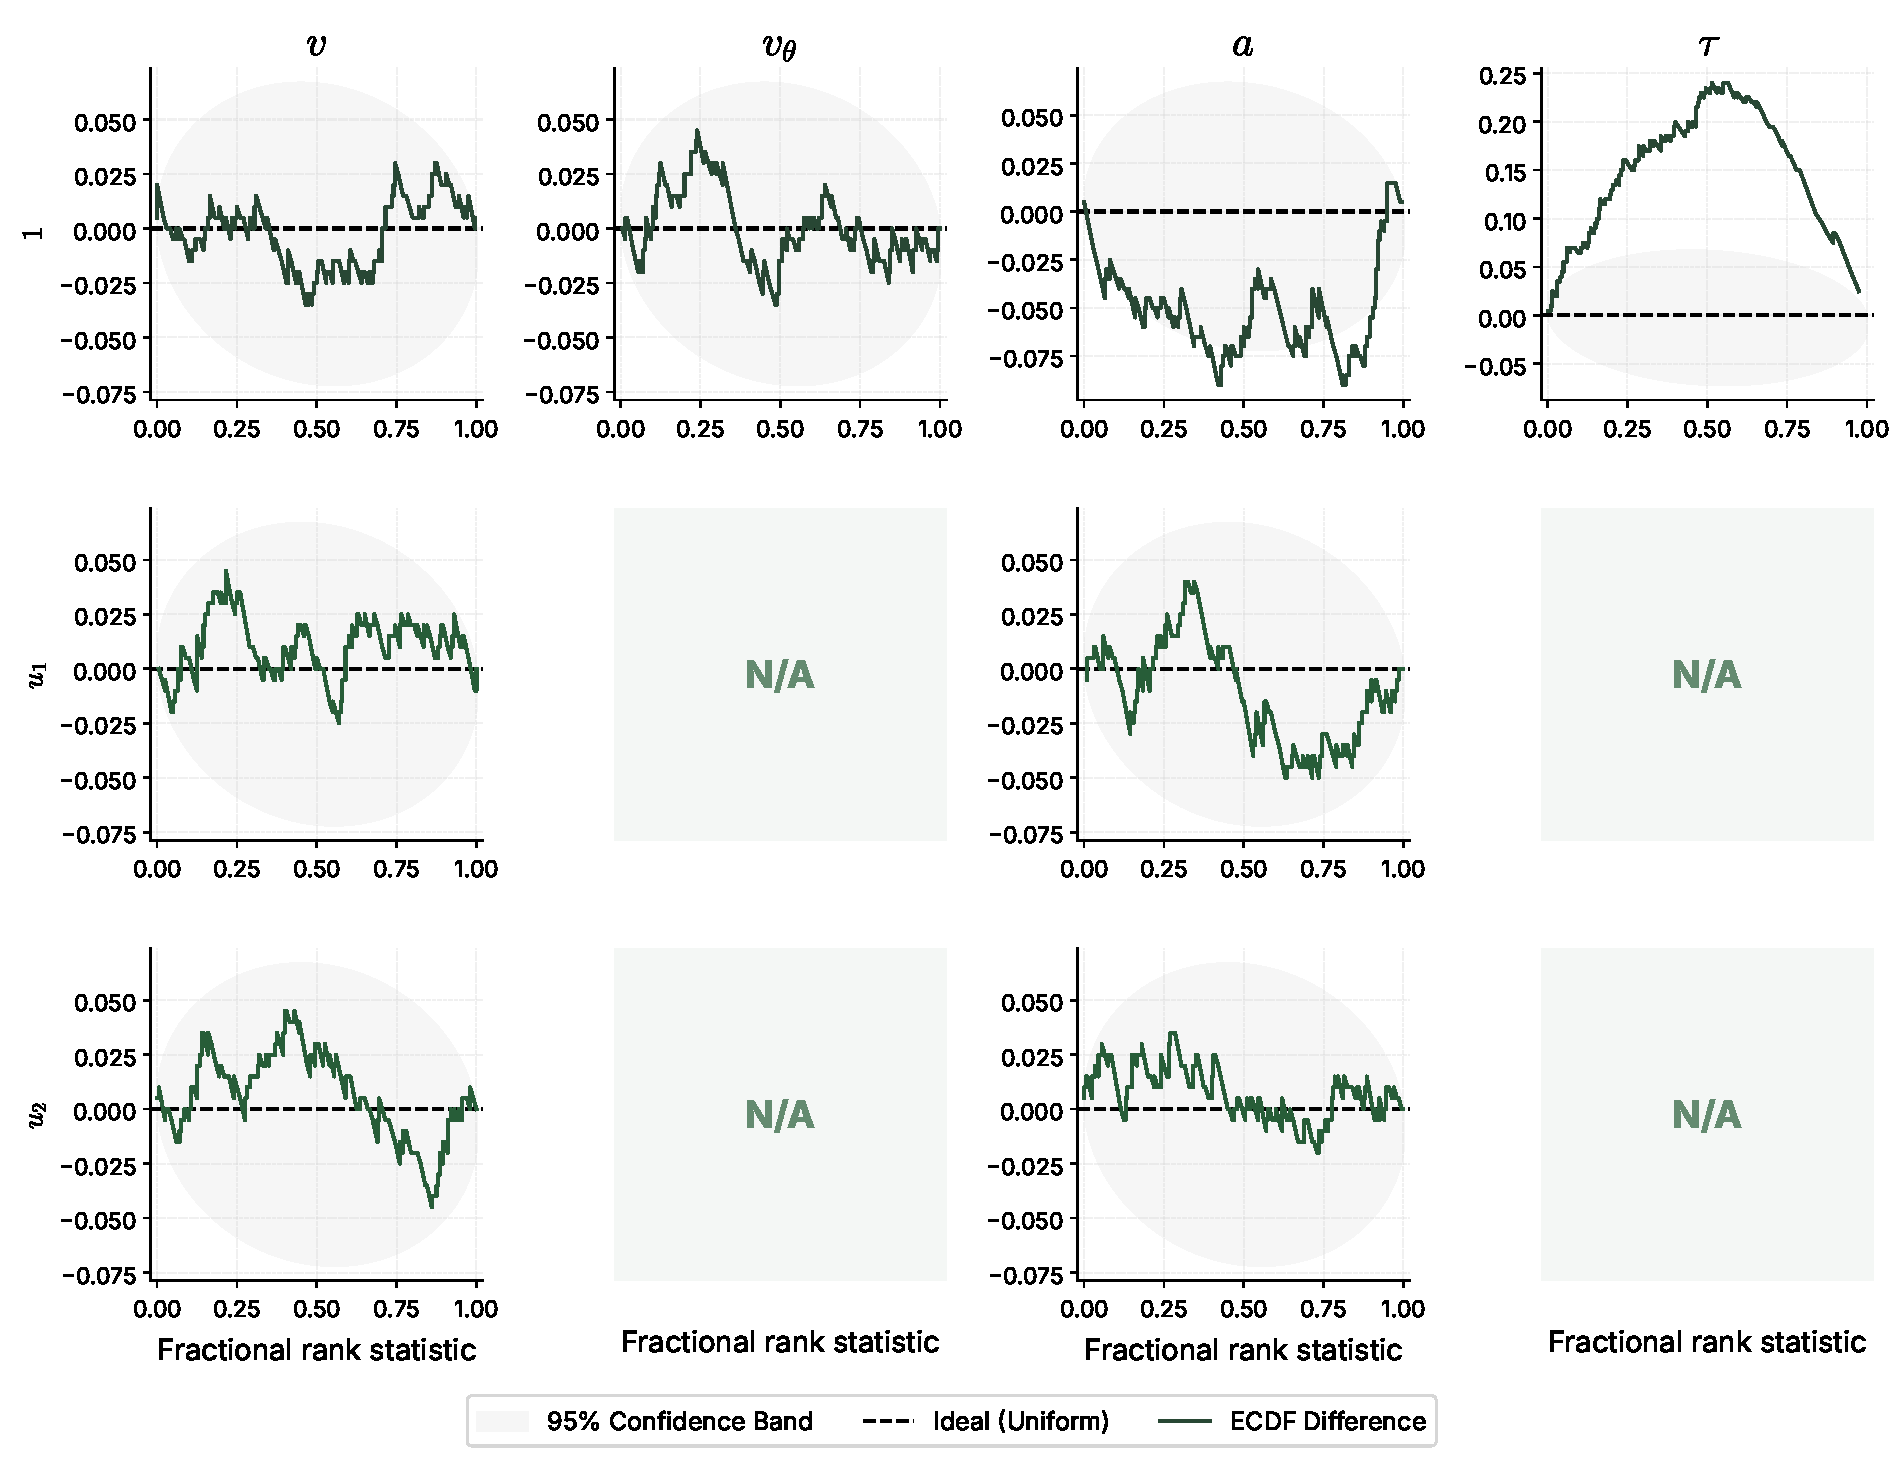
\includegraphics[width=\textwidth,height=0.3\textheight,keepaspectratio]{cdm/fixed_regressed/bf_ecdf.pdf}\par\vspace{1ex}
  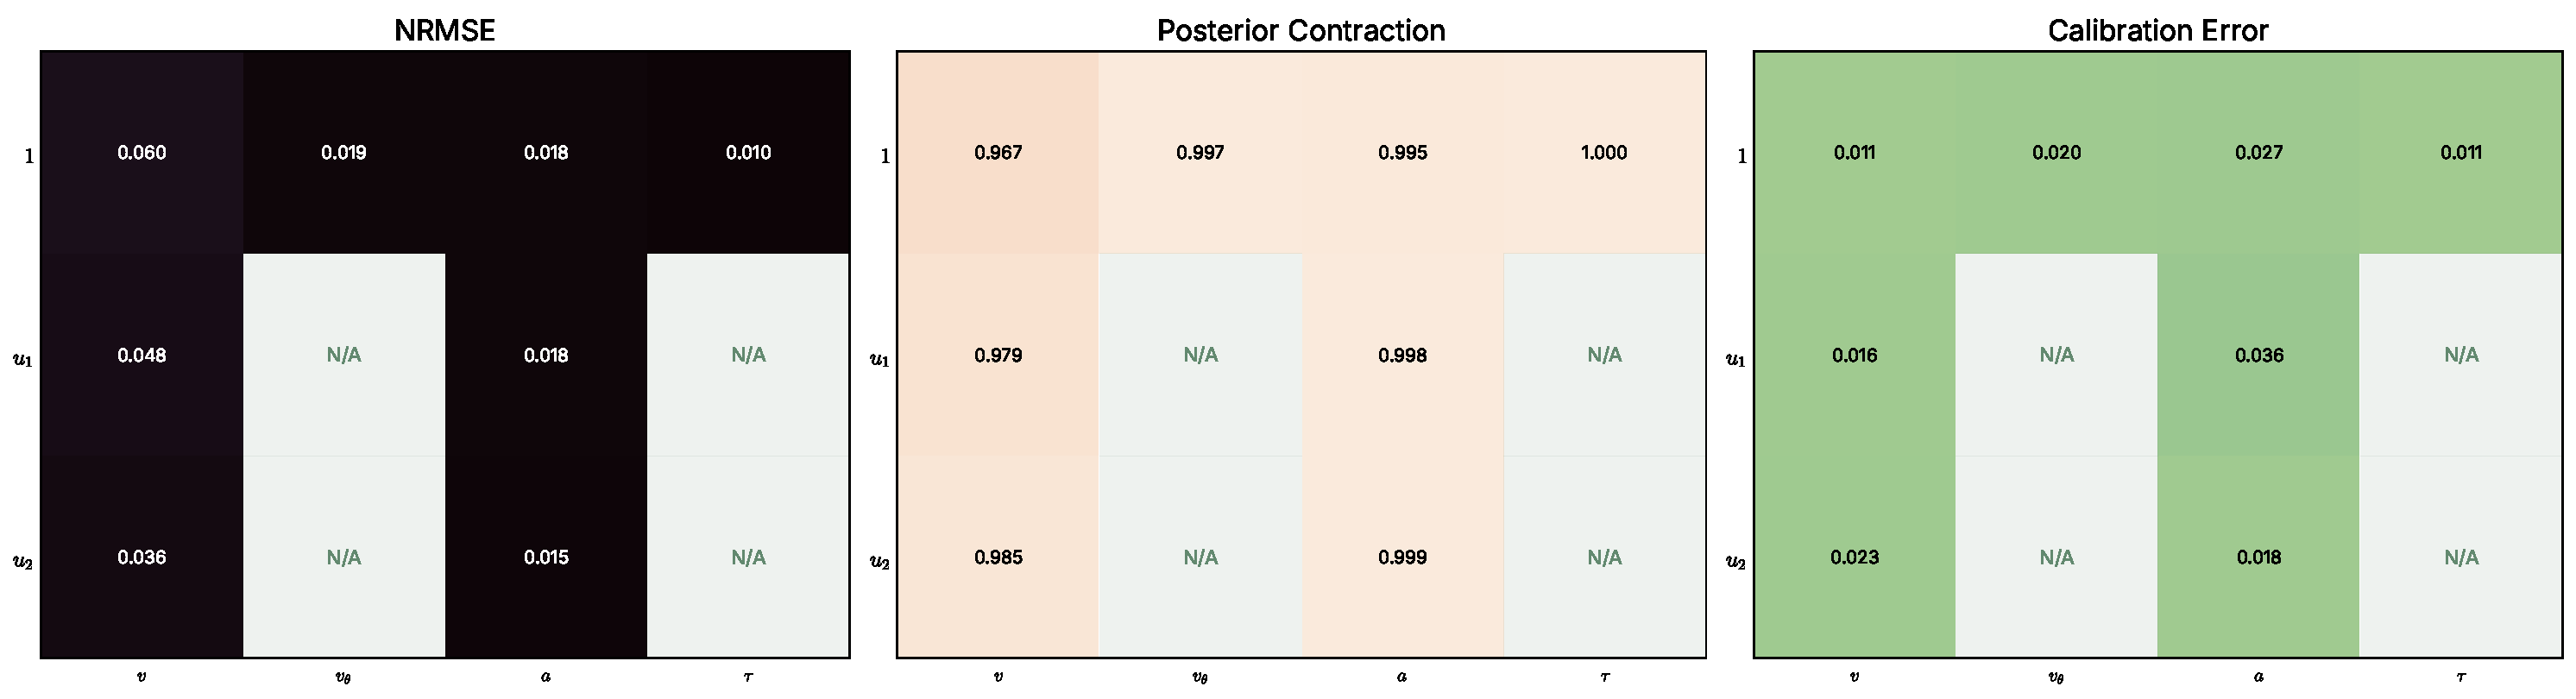
\includegraphics[width=\textwidth]{cdm/fixed_regressed/bf_metrics.pdf}
  \caption{\textbf{CDM, \emph{fixed + regressed} design: BayesFlow baseline.} Recovery (top), calibration (middle), metrics (bottom). $s_v$ and $s_\tau$ are fixed at 0 and not estimated; $v$ and $a$ carry slopes on $u_1$ and $u_2$ (8 coefficients shown). Layout and encoding as in Figure~\ref{fig:app1-ddm-intercept-only-cf}.}
  \label{fig:app1-cdm-fixed-regressed-bf}
\end{figure}

\begin{figure}[p]
  \centering
  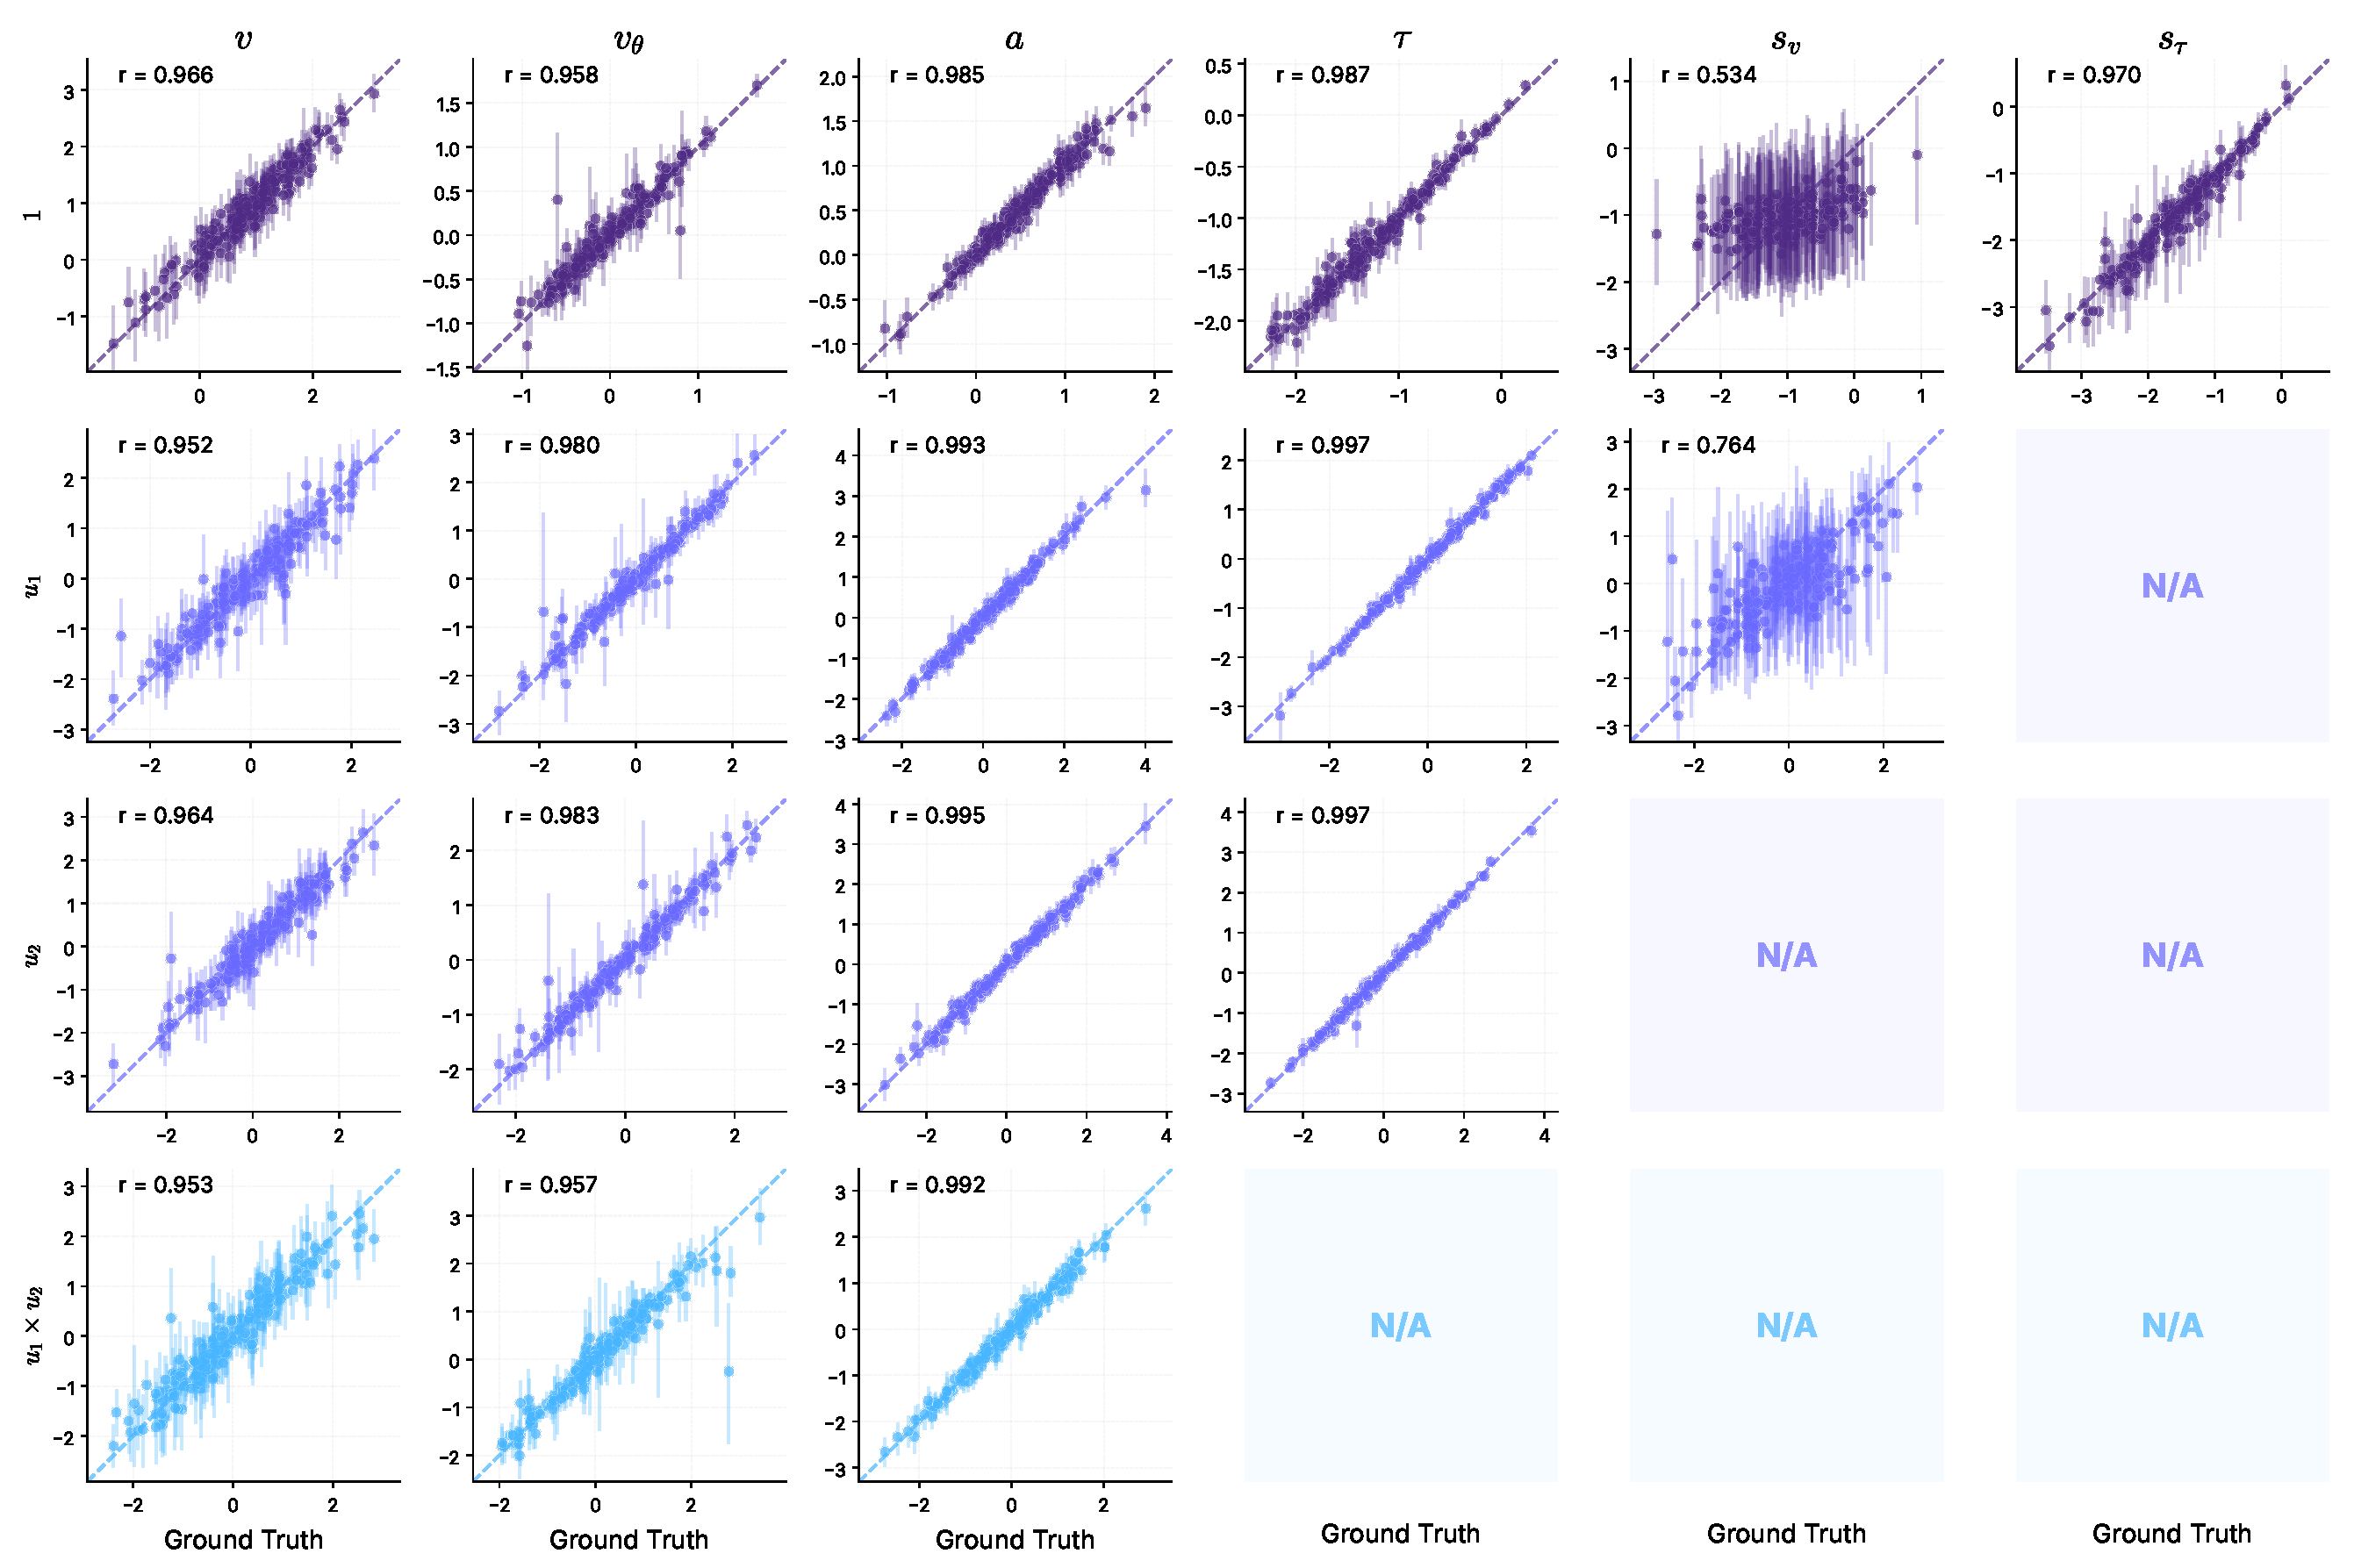
\includegraphics[width=\textwidth,height=0.3\textheight,keepaspectratio]{cdm/interaction/cf_recovery.pdf}\par\vspace{1ex}
  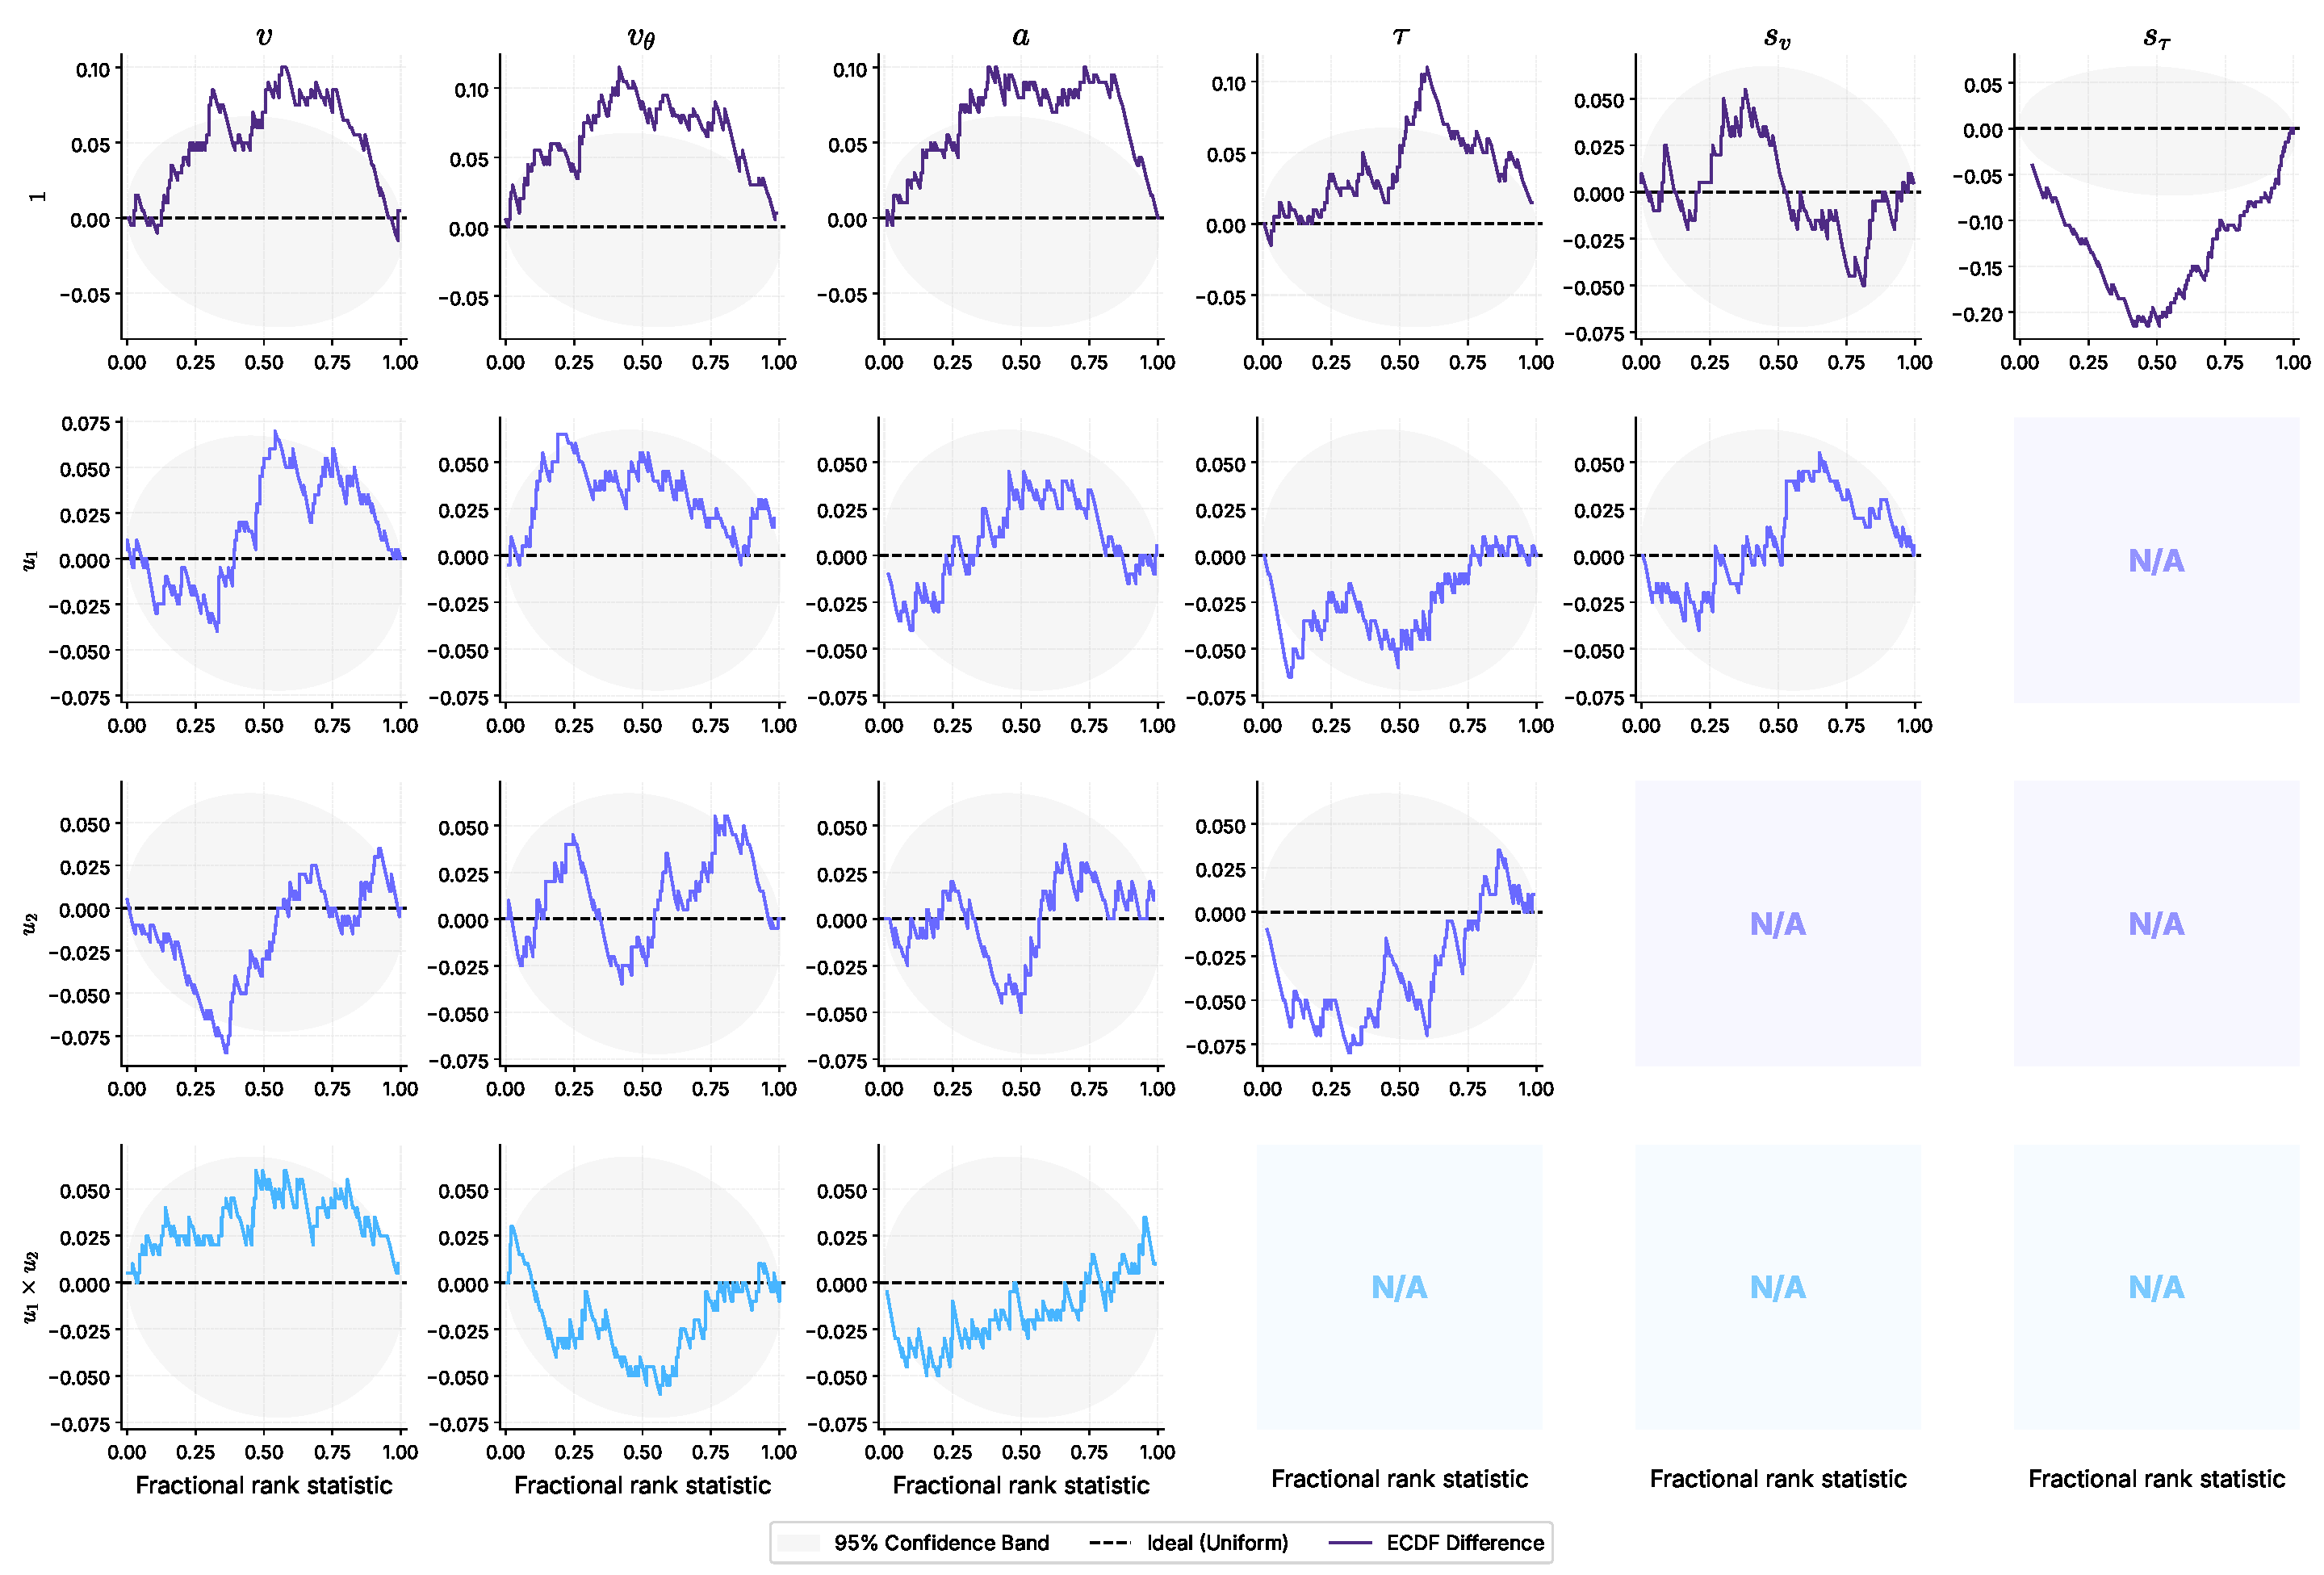
\includegraphics[width=\textwidth,height=0.3\textheight,keepaspectratio]{cdm/interaction/cf_ecdf.pdf}\par\vspace{1ex}
  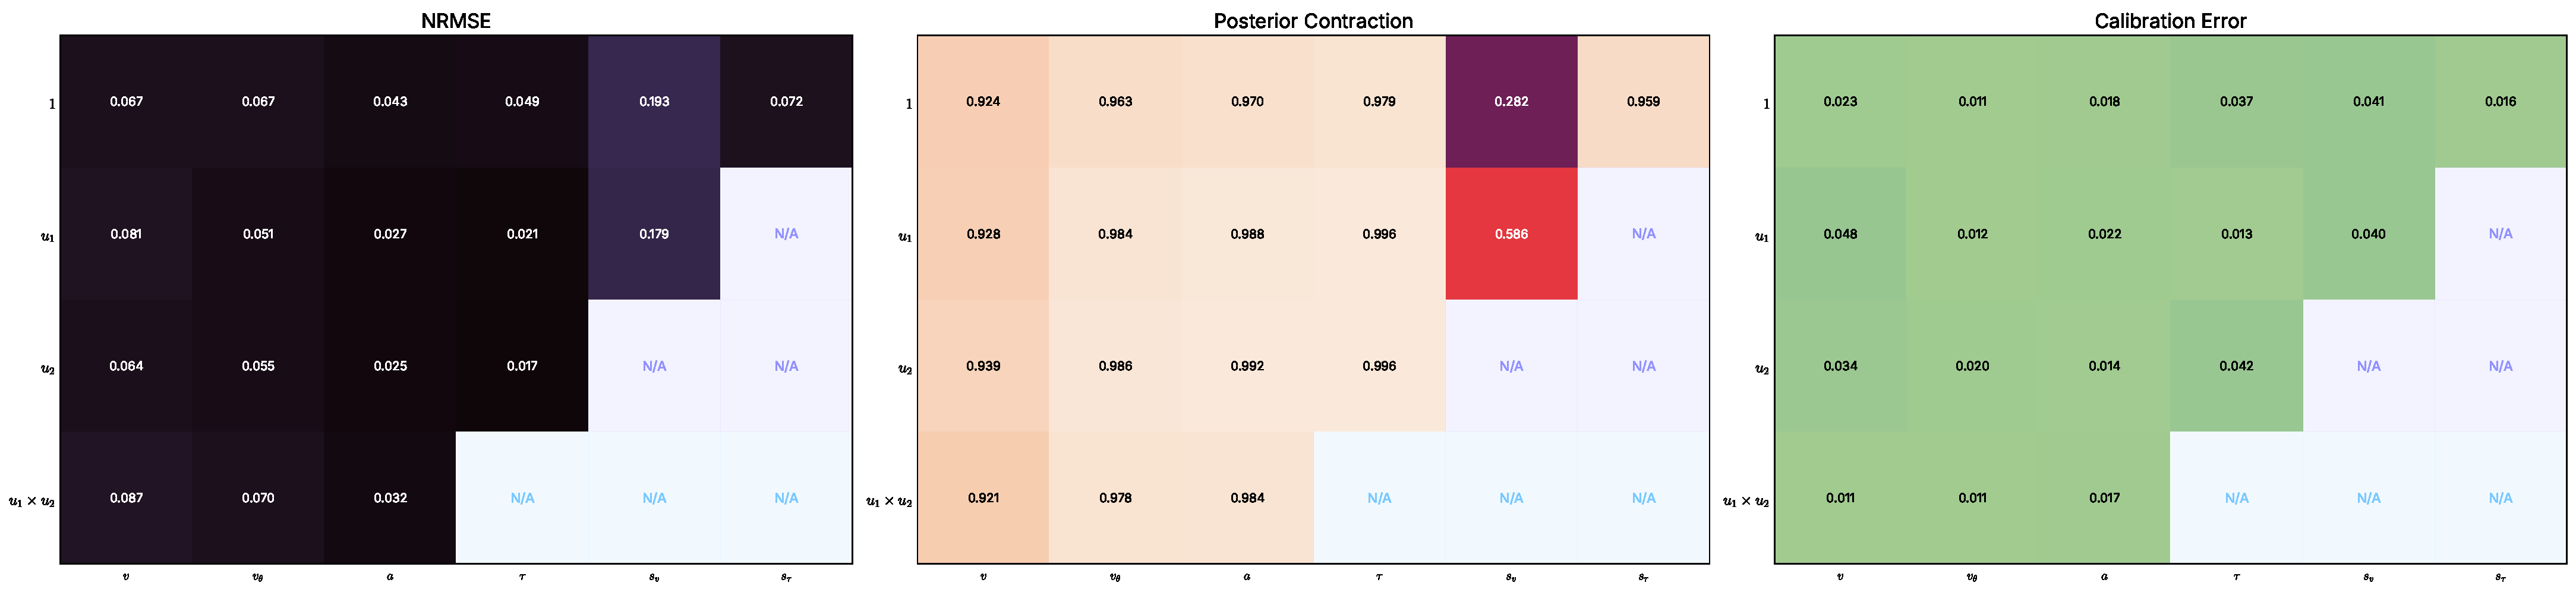
\includegraphics[width=\textwidth]{cdm/interaction/cf_metrics.pdf}
  \caption{\textbf{CDM, \emph{interaction} design: CogFormer.} Recovery (top), calibration (middle), metrics (bottom). $v$, $v_\theta$, $a$, $\tau$ and $s_v$ carry slopes on $u_1$; $v$, $v_\theta$, $a$ and $\tau$ carry slopes on $u_2$; $v$, $v_\theta$ and $a$ on the product $u_1 u_2$ (18 coefficients shown). Layout and encoding as in Figure~\ref{fig:app1-ddm-intercept-only-cf}.}
  \label{fig:app1-cdm-interaction-cf}
\end{figure}

\begin{figure}[p]
  \centering
  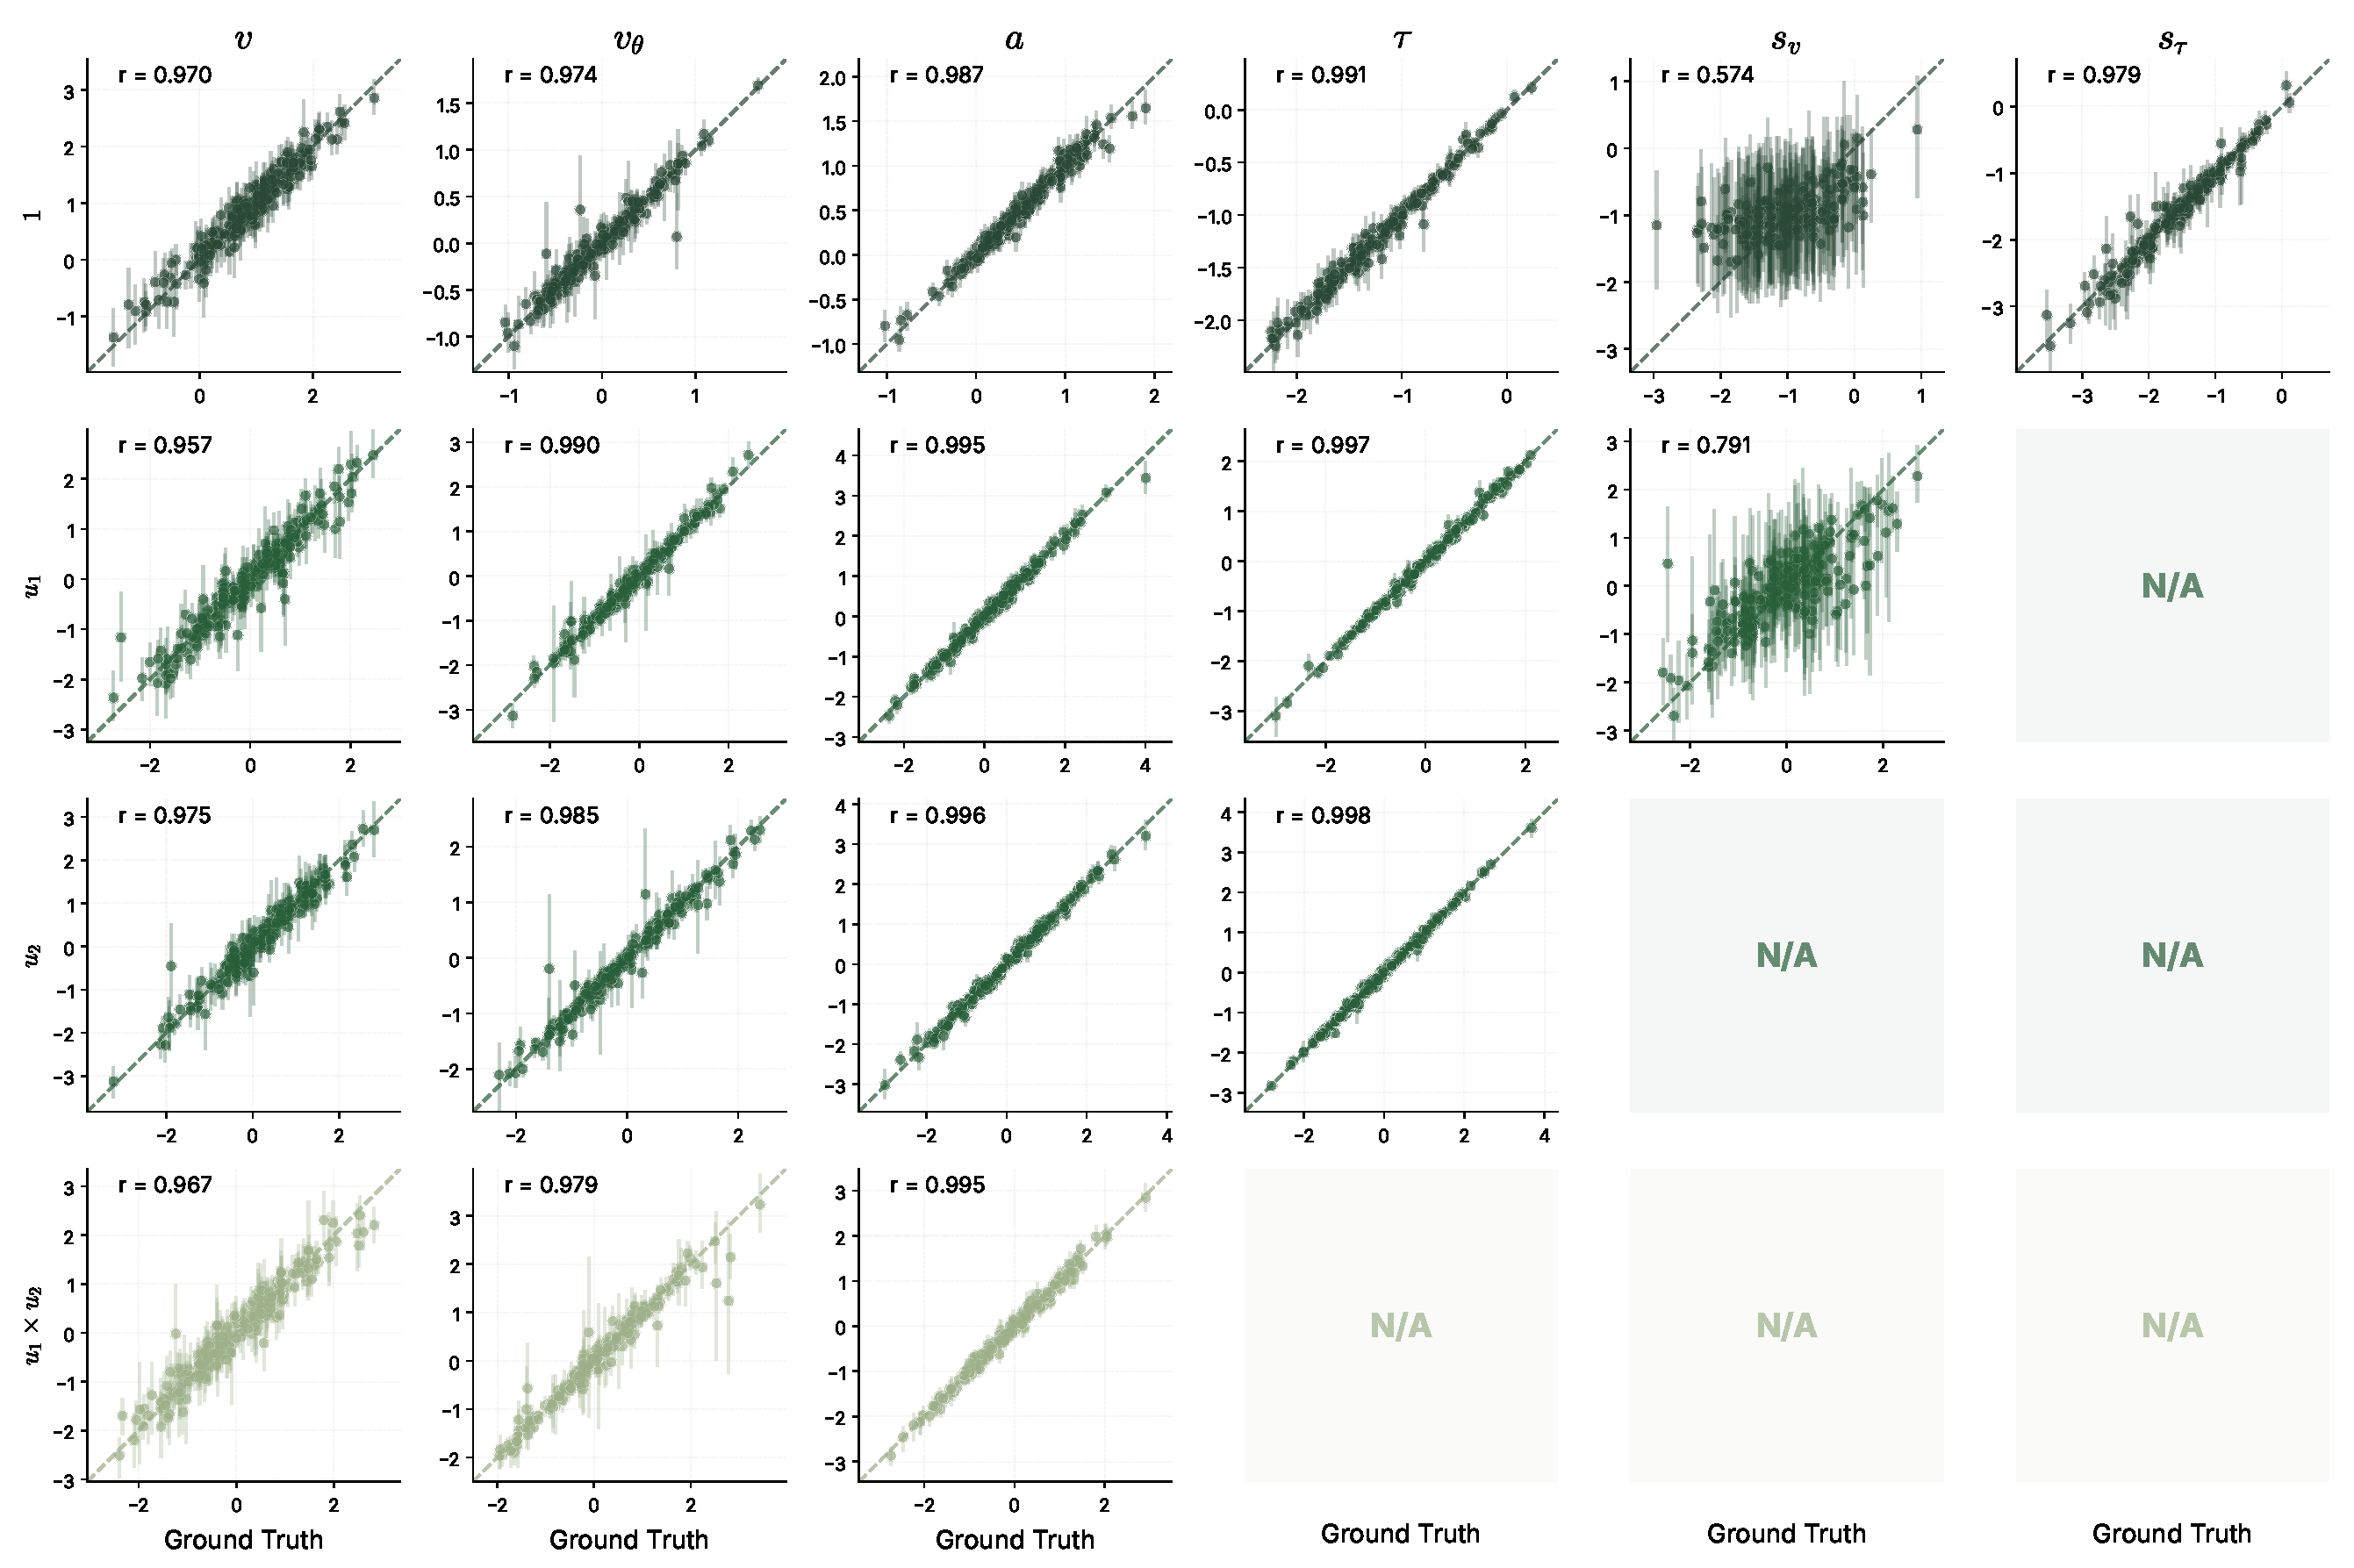
\includegraphics[width=\textwidth,height=0.3\textheight,keepaspectratio]{cdm/interaction/bf_recovery.pdf}\par\vspace{1ex}
  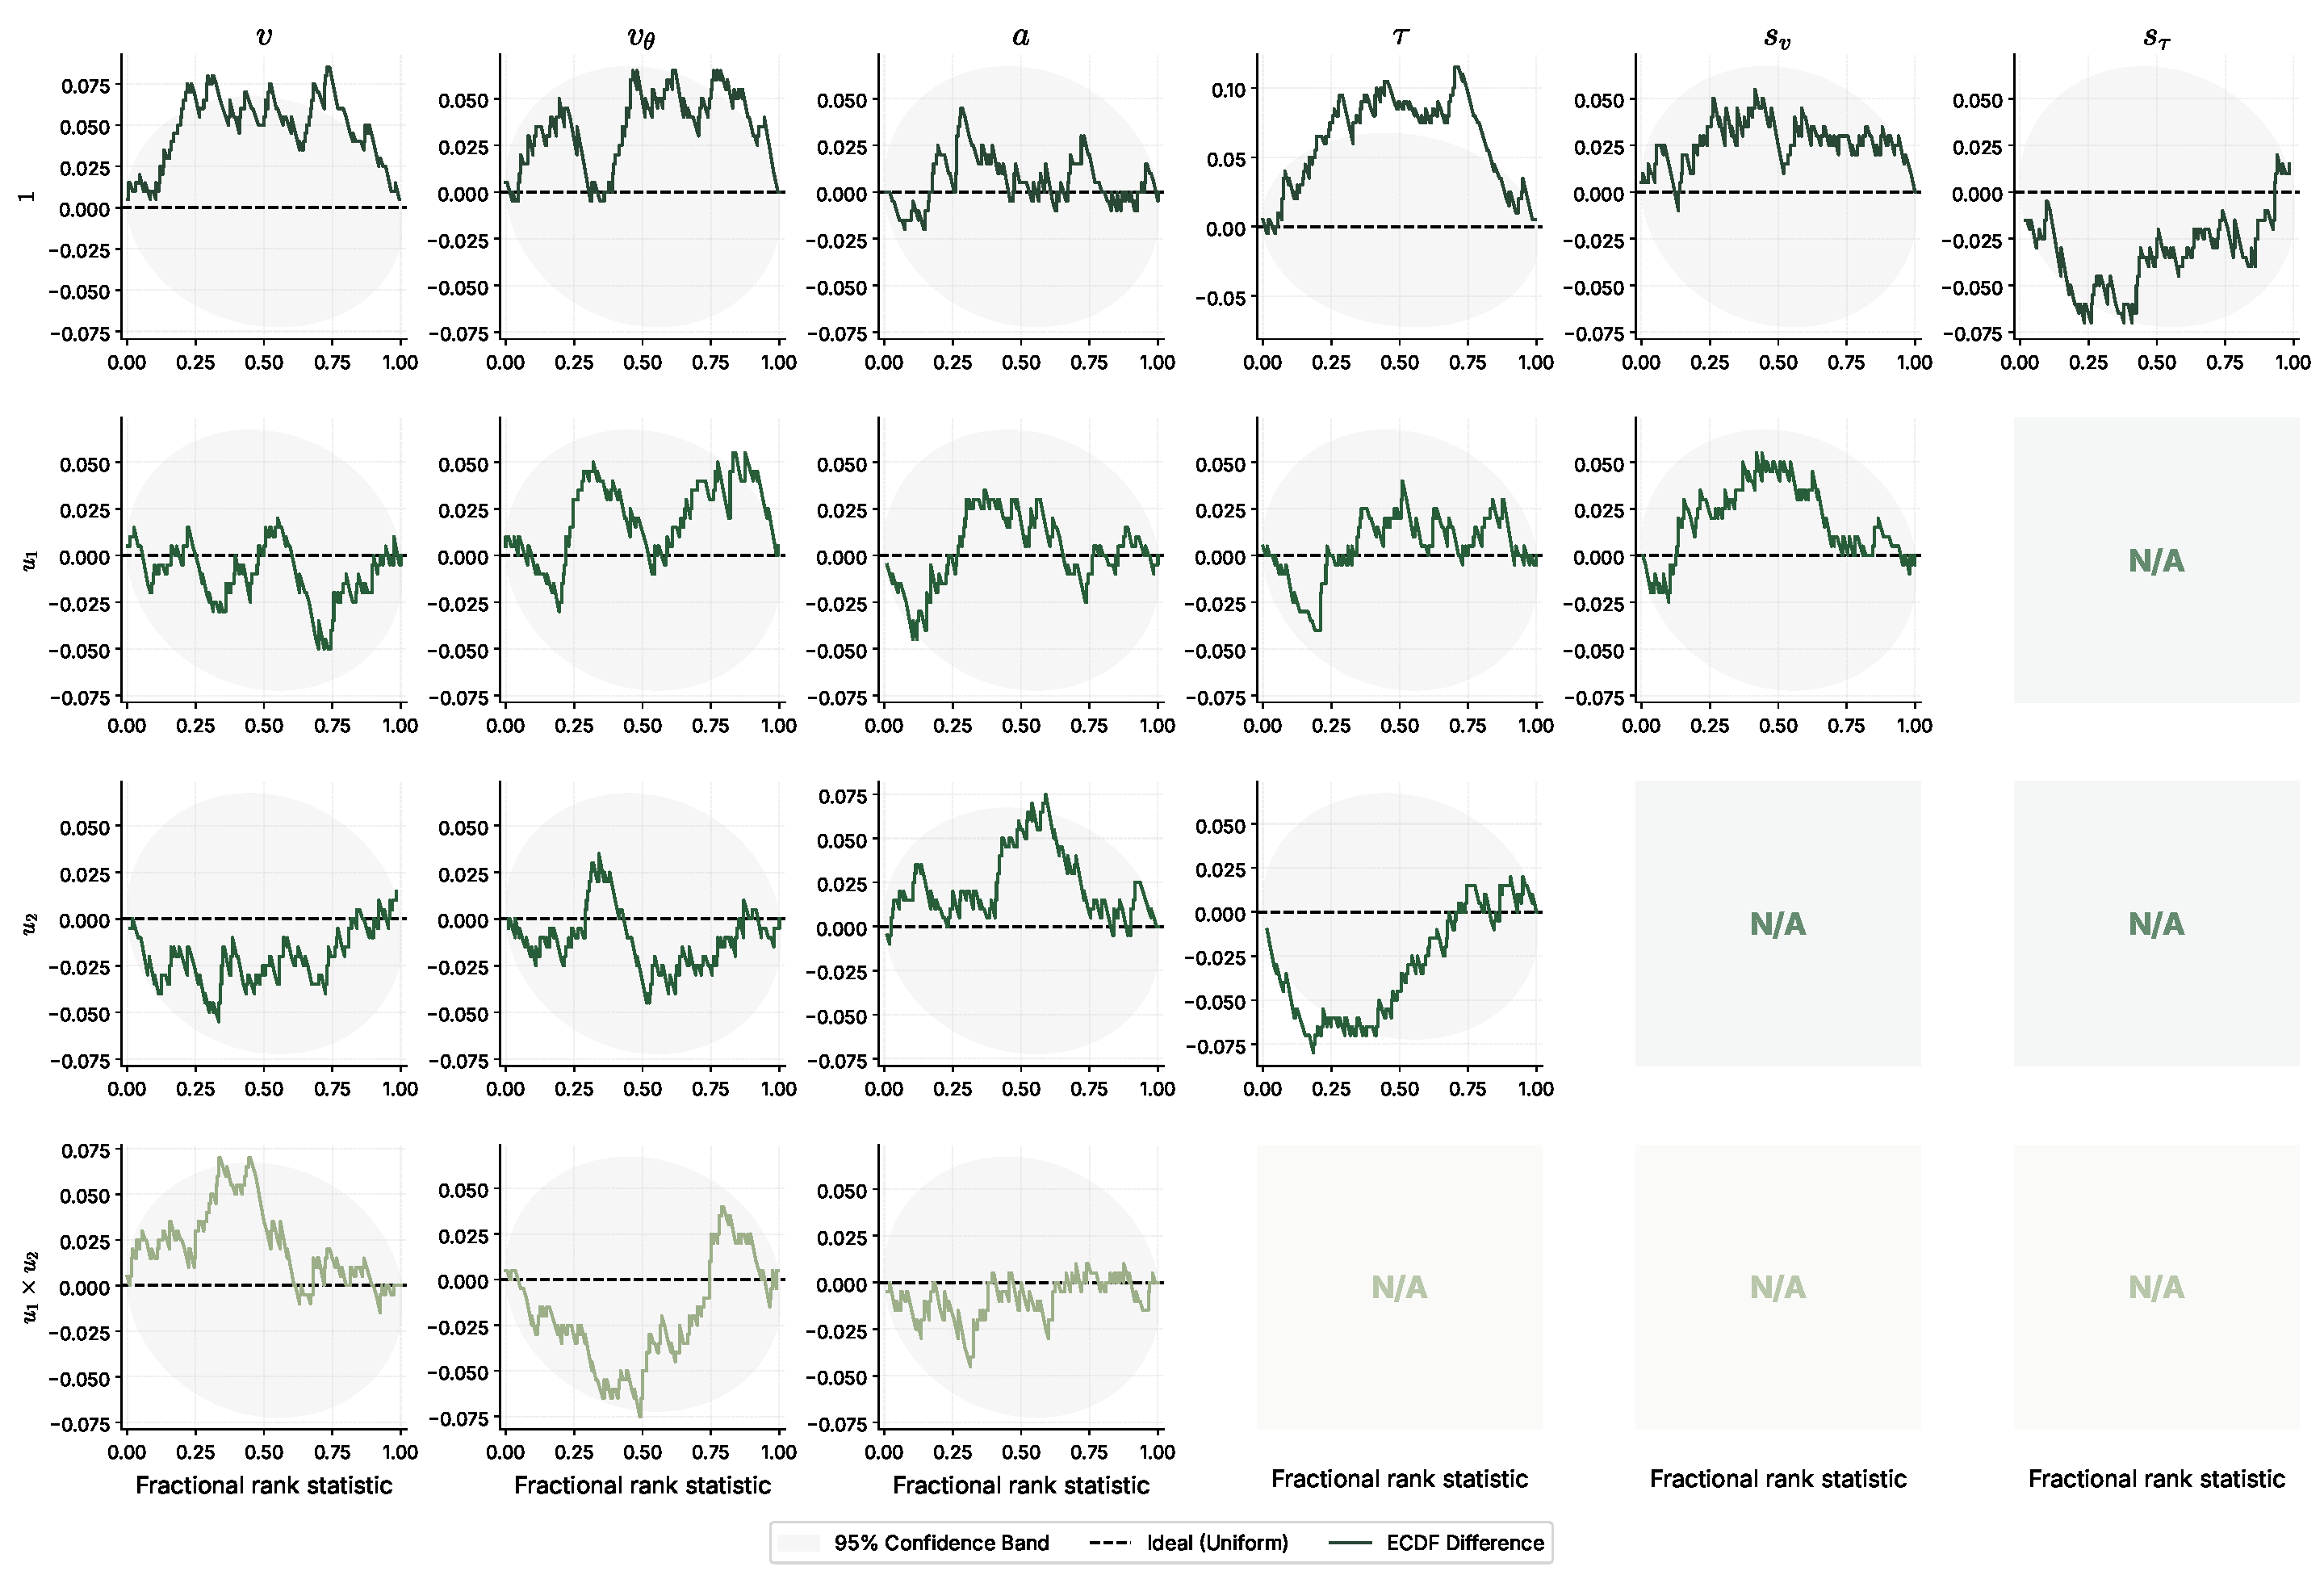
\includegraphics[width=\textwidth,height=0.3\textheight,keepaspectratio]{cdm/interaction/bf_ecdf.pdf}\par\vspace{1ex}
  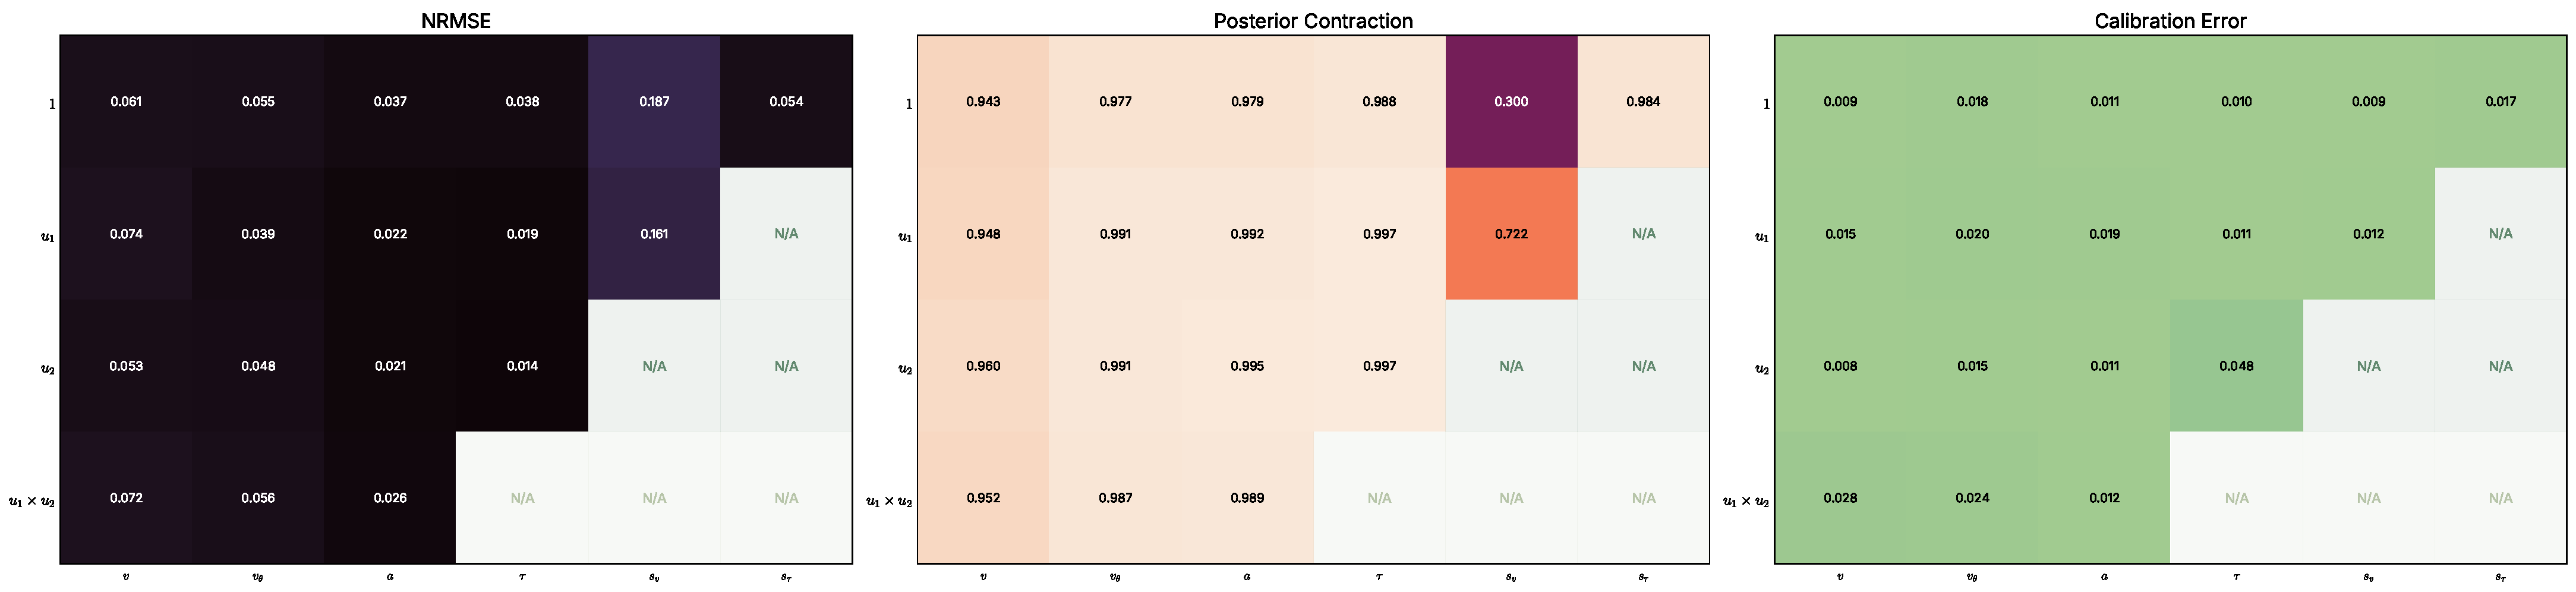
\includegraphics[width=\textwidth]{cdm/interaction/bf_metrics.pdf}
  \caption{\textbf{CDM, \emph{interaction} design: BayesFlow baseline.} Recovery (top), calibration (middle), metrics (bottom). $v$, $v_\theta$, $a$, $\tau$ and $s_v$ carry slopes on $u_1$; $v$, $v_\theta$, $a$ and $\tau$ carry slopes on $u_2$; $v$, $v_\theta$ and $a$ on the product $u_1 u_2$ (18 coefficients shown). Layout and encoding as in Figure~\ref{fig:app1-ddm-intercept-only-cf}.}
  \label{fig:app1-cdm-interaction-bf}
\end{figure}
